% main.tex
% Compile with: XeLaTeX
\documentclass[12pt,a4paper]{report}

% =========================
% Basic layout / font
% =========================
\usepackage[fontsize=13pt]{scrextend}      % font size helper
\usepackage[a4paper,top=2cm,bottom=2cm,left=3cm,right=2cm]{geometry}

% XeLaTeX font loader
\usepackage{fontspec}
\setmainfont{Times New Roman}

% system font

% Language
\usepackage[vietnamese,english]{babel}     % nếu muốn đổi sang polyglossia, báo mình

% =========================
% Spacing & paragraph
% =========================
\usepackage{setspace}
\onehalfspacing
\setlength{\parindent}{0pt}
\setlength{\parskip}{0.5\baselineskip}

% =========================
% Math
% =========================
\usepackage{amsmath}        
\usepackage{unicode-math}
% \setmathfont{Latin Modern Math}
\usepackage{textcomp}
% =========================
% Figures, tables, graphics
% =========================
\usepackage{graphicx}
\usepackage{caption}
\usepackage{subcaption}
\usepackage{float}           % [H]
\usepackage{booktabs}
\usepackage{threeparttable}
\usepackage{longtable}
\usepackage{tabularx}
\usepackage{enumitem}
\usepackage{xurl}
\emergencystretch=2em

% =========================
% TikZ / drawing
% =========================
\usepackage{tikz}
\usetikzlibrary{shapes.geometric, arrows.meta, positioning}


% For cover background frames
\usepackage{eso-pic}

% =========================
% Lists, algorithms, code
% =========================
\usepackage{enumitem}
\setlist{nolistsep}
\usepackage[ruled,vlined,linesnumbered]{algorithm2e}
\usepackage{listings}
\usepackage{algorithmic}
\usepackage{array}

% =========================
% TOC / headings
% =========================
\usepackage{tocloft}
\usepackage{titlesec}
\titlespacing*{\section}{0pt}{*0.8}{*0.4}
\titlespacing*{\subsection}{0pt}{*0.5}{*0.2}
\usepackage{etoolbox}
\patchcmd{\section}{\par}{\medskip}{}{}
\patchcmd{\subsection}{\par}{\medskip}{}{}

% =========================
% Bibliography
% =========================
% You used IEEEtran as bibliography style below (numeric). Configure natbib accordingly.
\usepackage[numbers,sort&compress]{natbib}

% =========================
% Header / footer
% =========================
\usepackage{fancyhdr}
\usepackage{lastpage}

% =========================
% Hyperlinks (load late)
% =========================
\usepackage[hidelinks]{hyperref}
\hypersetup{
  colorlinks=true,
  linkcolor=black,
  citecolor=black,
  urlcolor=black
}
% =========================
% Cover variables (edit here)
% =========================
\newcommand{\ReportTitle}{DOMAIN GENERALIZATION FOR ADVERSARIAL ROBUSTNESS}
\newcommand{\CouncilName}{}
\newcommand{\SupervisorOne}{Nguyễn An Khương}
\newcommand{\SupervisorTwo}{Văn Minh Hào}
\newcommand{\ReviewerName}{...}
\newcommand{\StudentOneName}{Nguyễn Anh Kiệt}
\newcommand{\StudentOneID}{2252403}
\newcommand{\StudentTwoName}{Lê Văn Đức Anh}
\newcommand{\StudentTwoID}{2252027}
\newcommand{\StudentThreeName}{Nguyễn Tiến Thành}
\newcommand{\StudentThreeID}{2053437}
\newcommand{\CoverPlaceTime}{HO CHI MINH CITY, May 2026}


% =========================
% Misc
% =========================
\usepackage{xcolor}
\usepackage{lscape}
\usepackage{microtype}      


% =========================
% Document
% =========================
\begin{document}

% ---------- INS SIGNATURE ----------
% ========== COVER PAGE ==========
% frontmatter.tex
\begin{titlepage}
\AddToShipoutPictureBG*{%
    \AtPageLowerLeft{%
        \begin{tikzpicture}[overlay]
            % Outer frame with width 2pt
            \draw[line width=3pt]
            (3cm, 2cm) rectangle (\paperwidth-2cm, \paperheight-2cm);
            % Inner frame with width 1pt
            \draw[line width=1pt]
            (3.1cm, 2.1cm) rectangle (\paperwidth-2.1cm, \paperheight-2.1cm);
        \end{tikzpicture}%
    }%
}

\begin{center}
    \vspace*{0cm}
    \vspace{-0.3cm}

    \fontsize{15pt}{18pt}\selectfont
    \textbf{VIETNAM NATIONAL UNIVERSITY HO CHI MINH CITY}
    
    \textbf{HO CHI MINH CITY UNIVERSITY OF TECHNOLOGY}
    
    \textbf{FACULTY OF COMPUTER SCIENCE AND ENGINEERING}
    \begin{figure}[H]
        \centering
        
\includegraphics[scale=0.3]{figures/Logo_BK.png}
    \end{figure}

    \textbf{REPORT}

    \textbf{CAPSTONE PROJECT}

    \textbf{SEMESTER 252 ACADEMIC YEAR 2025-2026}
    \vspace{-0.3cm}

    \rule{0.8\textwidth}{0.5pt}
    
    \fontsize{20pt}{18pt}\selectfont
    \textcolor{blue}{\textbf{\MakeUppercase{DOMAIN GENERALIZATION FOR ADVERSARIAL ROBUSTNESS}}}
    
    \vspace{-0.3cm}

    \rule{0.8\textwidth}{0.5pt}

    \vspace{-0.3cm}

    \fontsize{15pt}{18pt}\selectfont
    \textbf{MAJOR: COMPUTER SCIENCE}

    \begin{tabular}{l l}
        \textbf{COUNCIL:} &  \\
    \textbf{SUPERVISOR(s):} &
        \begin{tabular}[t]{@{}l@{}}
          \SupervisorOne \\
          \SupervisorTwo
        \end{tabular} \\
    \textbf{REVIEWER:} &  \\

    \end{tabular}  
    \vspace{-0.3cm}
    
    \textbf{------o0o------}

    \vspace{-0.3cm}

      \begin{tabular}{l l}
        \textbf{STUDENT 1:} & \StudentOneName{} - \StudentOneID \\
        \textbf{STUDENT 2:} & \StudentTwoName{} - \StudentTwoID \\
        \textbf{STUDENT 3:} & \StudentThreeName{} - \StudentThreeID \\
      \end{tabular}
    
    \vfill

    {\CoverPlaceTime}

\end{center}
\end{titlepage}


% ---------- INS SIGNATURE ----------
\chapter*{Instructor’s Signature}

\vspace{1cm}

\makebox[0.7\linewidth][l]{\hrulefill} Date: \makebox[0.2\linewidth][l]{\hrulefill}

    \begin{flushleft}
     NGUYỄN AN KHƯƠNG (Instructor)\\
    \makebox[0.45\linewidth][l]{\hrulefill} \\
    Faculty of Computer Science and Engineering
    \end{flushleft}


% ---------- DECLARATION ----------
\chapter*{Declaration of Authenticity}

We declare that we solely conducted this specialized project, under the supervision of Dr. Nguyen An Khuong at the Faculty of Computer Science and Engineering, Vietnam National University - Ho Chi Minh City University of Technology and Mr. Van Minh Hao at University of Arkansas.
 
\noindent We have taken care to properly acknowledge and document all external sources and references used in the project.
 
\noindent If there is any instance of plagiarism, we are ready to accept the consequences. Ho Chi Minh City University of Technology - Vietnam National University HCMC will not be held responsible for any copyright violations that may have occurred during our research.

\vspace{2cm}

\begin{flushright}
\begin{tabular}{c}
    Ho Chi Minh City, May 2026 \\
    \textit{\textbf{Authors}} 
    
\end{tabular}
\end{flushright}


% ---------- ACKNOWLEDGEMENT ----------
\chapter*{Acknowledgement}

We would like to express our appreciation to Dr. Nguyen An Khuong for his invaluable guidance. Our research has greatly benefited from his deep knowledge, perceptive criticism, and constant support.

\noindent Besides, we are grateful for the help from Mr. Van Minh Hao for valuable comments for research aspect and our proposed pipeline, including pointing out strengths as well as weaknesses of previous works on adversarial attack so that we can elaborate on our ideas more effectively.

\noindent In addition, we would like to extend our gratitude to our family. Their unwavering faith in our abilities and constant encouragement have been our pillars of strength. Their belief in our potential has been a constant source of motivation and resilience. We are forever grateful for their love and support.


% ---------- ABSTRACT ----------
\chapter*{Abstract}

This thesis addresses the critical vulnerability of deep learning models to adversarial perturbations, particularly the limitation where standard defense mechanisms fail to generalize across different threat models. Our research proposes a novel perspective that treats distinct families of adversarial attacks as separate "domains," aiming to identify and quantify the "cross-attack robustness gap" inherent in current training paradigms.

\noindent We establish a comprehensive experimental framework to evaluate the transferability of robustness across diverse adversarial environments. By subjecting models trained on specific perturbation norms to a wide spectrum of unseen attack algorithms, the study systematically measures the performance degradation that occurs when shifting between these domains.

\noindent Ultimately, this quantitative analysis serves as the empirical foundation for the subsequent phase of research. By characterizing the domain shifts between attack families, we pave the way for integrating Domain Generalization principles into adversarial training. This progression aims to directly mitigate the observed robustness gaps, ensuring that future models can effectively generalize to unforeseen and heterogeneous adversarial scenarios.

% ---------- CONTENT ----------
% ========== TABLES OF CONTENTS / LISTS ==========
\tableofcontents
\clearpage
\listoffigures
\clearpage
\listoftables
\clearpage

% ---------- List of Abbreviations ----------
\chapter*{List of Abbreviations}

\begin{longtable}{|p{3cm}|p{7cm}|} % Adjust column widths as needed
\hline
\textbf{Abbreviation} & \textbf{Definitions} \\
\hline
AA & AutoAttack \\
    \hline
    AT & Adversarial Training \\
    \hline
    CW & Carlini--Wagner \\ 
    \hline
    DG & Domain Generalization \\
    \hline
    DNN & Deep Neural Network \\
    \hline
    FGSM & Fast Gradient Sign Method \\
    \hline
    IRM & Invariant Risk Minimization \\
    \hline
    PGD & Projected Gradient Descent \\
    \hline
    REx & Risk Extrapolation \\
\hline


\end{longtable}








% ---------- MAIN CONTENT ----------
\chapter{Introduction}
\label{chap:introduction}

\section{Adversarial Robustness and the Cross-Attack Gap}

Modern neural networks achieve high accuracy on standard image classification
benchmarks, yet they can be sensitive to small, carefully crafted perturbations
of their inputs.  These adversarial perturbations are often imperceptible to
human observers, but they can change the model's prediction with high
reliability.  The phenomenon has motivated a large body of work on adversarial
training, which augments the training process with adversarial examples so that
the resulting classifier learns to resist such perturbations.

Adversarial training has become the dominant empirical defense against
adversarial attacks.  However, the effectiveness of adversarial training
typically depends on the attack used during training.  Different attacks employ
different perturbation norms, optimization objectives, and step-size schedules,
and a model trained against one attack may not transfer its robustness to
attacks with different characteristics.  For example, a model that is robust
under a projected gradient descent attack in the $\ell_\infty$ norm may remain
vulnerable to optimization-based attacks in the $\ell_2$ norm, and vice versa.
This creates what this report calls the \emph{cross-attack robustness gap}: the
difference in a model's robustness when evaluated under attacks that differ from
the one used during training.

The cross-attack gap is not merely a theoretical concern.  Evaluation suites
that include attacks from multiple norms, step counts, and optimization
objectives routinely show that single-attack adversarial training produces
models whose robustness is concentrated on the source threat family.  Once the
evaluation moves outside that family, performance can degrade substantially.
This observation suggests that robustness should be measured not by a single
attack score but by how well a model performs across a diverse set of threat
models.

One natural response is to train the model against multiple attacks
simultaneously.  Multi-attack adversarial training constructs adversarial
examples from more than one source attack during each training step and averages
the resulting losses.  This strategy provides broader coverage than single-attack
training, but it treats all attack-induced examples uniformly.  If some attacks
or attack-induced subgroups are systematically harder than others, uniform
averaging can hide those failure modes behind an improved overall mean.

This report focuses on improving the balance of robustness across a fixed attack
suite rather than claiming universal robustness against arbitrary perturbations.
The experimental scope is bounded to CIFAR-10 image classification with a
defined set of evaluation attacks, and the claims are conditioned on the
specific training and evaluation protocol described in later chapters.  This
motivates the central question of this report: whether adversarial training can
be made less dependent on a single source attack by treating attacks and
attack-induced failures as structured domains.

\section{Stage 1 Findings and Their Limitations}

The present work continues from a Stage~1 investigation that diagnosed
attack-dependent robustness under single-attack adversarial training.  Stage~1
trained classifiers using individual source attacks and evaluated them against a
broader attack suite.  The main observation was that single-attack training
tends to specialize: a model trained against an $\ell_\infty$ source attack
achieved strong robustness under held-out $\ell_\infty$ attacks but weaker
performance under $\ell_2$ attacks, and symmetrically for an $\ell_2$ source
attack.

Stage~1 also established an evaluation discipline that carries forward into the
present report.  The attack suite, the use of repeated random seeds, and the
separation of source and held-out attacks were all informed by Stage~1
observations.  However, Stage~1 was primarily evaluative and diagnostic: it
measured the cross-attack gap but did not propose a training method to reduce
it.

The limitation of Stage~1 is therefore clear.  Diagnosis alone does not produce
a training intervention.  Knowing that single-attack robustness is
attack-dependent motivates the search for a training strategy that balances
robustness across attacks, but the strategy itself must be designed, implemented,
and tested.  Stage~2 addresses this gap by introducing a progression of
multi-attack and group-aware training methods, evaluated under a controlled
experimental protocol.

The present report therefore moves from diagnosis to intervention.  It takes the
cross-attack gap observed in Stage~1 as its starting point and develops a
method that treats attack-induced adversarial examples as domain-like groups.
The goal is to shift training emphasis toward harder groups without abandoning
the stability of a uniform multi-attack baseline.

\section{Problem Statement}

The problem studied in this report is supervised image classification on
CIFAR-10, where a classifier is trained under adversarial examples generated by
two source attacks: PGD-$\ell_\infty$ and DDN-$\ell_2$.  Each source attack
induces a different distribution of adversarial examples, and these distributions
can be viewed as domain-like groups with distinct loss landscapes and failure
patterns.  The trained model is then evaluated under a broader suite of eight
attacks spanning both the $\ell_\infty$ and $\ell_2$ families, along with a
separate AutoAttack-$\ell_\infty$ stress test.

Uniformly averaging the losses across source attacks during training can hide
hard attacks, hard classes, or latent subgroups that consistently receive higher
loss.  If certain attack-induced regions are systematically underweighted, the
resulting model may appear robust on average while remaining vulnerable in
specific evaluation cells.  This motivates the need for a training objective
that can detect and emphasize difficult groups during optimization.

The problem studied in this report is not to solve adversarial robustness in
general, but to improve the balance of robustness across a predefined attack
suite under a reproducible training and evaluation protocol.  The goal is to
improve average robustness across seen and held-out attacks while avoiding severe
degradation on the hardest evaluation cases, all within the computational and
dataset constraints of CIFAR-10 and ResNet-18.

\section{Research Questions and Hypotheses}

This report is organized around four research questions, each targeting a
different aspect of cross-attack robustness.  These questions are designed so
that the experimental evidence in Chapter~\ref{chap:results_analysis} can
address them directly, and Chapter~\ref{chap:conclusion} can synthesize the
answers.

\textbf{RQ1: How large is the cross-attack robustness gap under single-attack
training?}  The hypothesis is that single-attack adversarial training will
produce attack-dependent robustness profiles, with each single-attack method
protecting its own source family more strongly than attacks outside that
training objective.

\textbf{RQ2: Does multi-attack training improve robustness across seen and
held-out attacks?}  The hypothesis is that Multi-AT, a uniform multi-attack
adversarial training baseline, will improve robustness balance compared with
single-attack baselines by covering both source threat geometries, though
uniform averaging may not fully remove hard attack-specific or class-specific
failure modes.

\textbf{RQ3: Can group-aware training improve robustness and stability beyond
uniform multi-attack training?}  The hypothesis is that AttackDRO++, which
discovers latent hard groups and upweights them during training, will improve
average robustness and training stability over Multi-AT in the main setting.
However, hardest-case robustness and transfer behavior should be interpreted
conservatively, as the advantage may be more limited under those evaluation
conditions.

\textbf{RQ4: Which design choices are responsible for the final behavior?}  The
hypothesis is that moderate cluster count, moderate anchor strength, and a
stable cluster-refresh schedule should produce better robustness balance than
extreme settings, providing practical configuration guidance for the method.

\section{Contributions of This Work}

This report makes the following contributions within the bounded experimental
setting of CIFAR-10 and ResNet-18:

\begin{enumerate}
\item It proposes an \emph{attacks-as-domains} framing for cross-attack
robustness, in which adversarial examples generated by different source attacks
are treated as domain-like groups whose losses can be balanced during training.

\item It implements a progression of training methods: a uniform Multi-AT
baseline, AttackDRO with group distributionally robust optimization (DRO) over
source attack identities, and AttackDRO++ with group DRO over discovered latent
clusters.

\item It introduces gradient fingerprint clustering features that augment the
standard penultimate representation with projected classifier-head gradients,
enabling the grouping mechanism to reflect optimization-level difficulty rather
than representation similarity alone.

\item It introduces a uniform-anchored training objective that keeps the
AttackDRO++ objective tied to the Multi-AT training signal while still allowing
difficult discovered groups to receive additional emphasis.

\item It evaluates the proposed method through a reproducible protocol that
includes aggregate whitebox comparisons, per-attack and per-class drilldowns,
graybox transfer analysis across independently trained surrogate models,
statistical significance testing with paired seeds, and hyperparameter
sensitivity studies.
\end{enumerate}

\section{Scope and Limitations}

The experimental scope of this report is bounded in several ways that should be
stated before the method and results chapters.

The dataset used throughout is CIFAR-10, a standard benchmark for adversarial
training research but a small, low-resolution image dataset.  The main
architecture is ResNet-18, adapted for CIFAR-10 resolution.  All central claims
are conditioned on this dataset and architecture combination.

The source attacks used during training are PGD-$\ell_\infty$ and
DDN-$\ell_2$.  The evaluation suite includes eight attacks spanning both
$\ell_\infty$ and $\ell_2$ families, plus a separate
AutoAttack-$\ell_\infty$ stress test that is reported independently from the
main aggregate metrics.  The evaluation does not include certified robustness,
full adaptive robustness, or robustness against attacks outside the defined
suite.

Graybox transfer evaluation is included, using independently trained surrogate
models from the same method families.  This tests whether robustness behavior
remains stable under transferred attacks, but it is still bounded to the chosen
model families and attack suite.  Supplementary architecture evidence from a
single WRN-28-10 run is provided in Appendix~\ref{app:extras}, but it is not
part of the main paired claims and does not support a broad architecture-level
generalization.

This report does not claim universal robustness.  It does not establish that the
proposed method generalizes to other datasets, architectures, or attack
configurations beyond those tested.  The conclusions are intended to be useful
within the defined protocol and to motivate further investigation under broader
conditions.

\section{Report Organization}

The remainder of this report is organized as follows.
Chapter~\ref{chap:background} provides the background needed to understand the
proposed method, covering adversarial attacks, adversarial training, distributionally
robust optimization (DRO), domain generalization, clustering,
and the statistical tools used for multi-seed evaluation.
Chapter~\ref{chap:related_work} reviews related work on multi-attack adversarial
training, group-aware robustness, domain generalization, and cluster-based
training, and identifies the remaining gap that this report addresses.

Chapter~\ref{chap:methodology} presents the proposed methodology in a
progression from the attacks-as-domains formulation through Multi-AT, AttackDRO,
and AttackDRO++, including gradient fingerprint clustering and the
uniform-anchored objective.  Chapter~\ref{chap:experimental_setup} defines the
experimental protocol: dataset, architecture, attack suite, training
configuration, hyperparameters, statistical significance protocol, evaluation
metrics, and graybox transfer design.

Chapter~\ref{chap:results_analysis} presents the results and analysis, moving
from aggregate whitebox robustness to class-wise drilldowns, graybox transfer,
and hyperparameter sensitivity studies.  Chapter~\ref{chap:conclusion} concludes
the report with answers to the research questions, a discussion of limitations,
and directions for future work.  The report therefore moves from motivation and
background to method design, then to a controlled empirical evaluation and a
final discussion of what the evidence supports.


%=========================
% CHAPTER 2 – BACKGROUND
%=========================
\chapter{Background}
\label{chap:background}

\section{Notation and Learning Setting}

This chapter fixes the technical vocabulary used by the later methodology and evaluation chapters. The goal is not to survey every defense or attack, but to define the optimization setting in which adversarial examples, multi-attack training, group reweighting, clustering, and multi-seed evaluation are used. The notation is kept deliberately close to the notation used in Chapters~\ref{chap:methodology} and~\ref{chap:experimental_setup}.

We consider supervised classification with input space $\mathcal{X}\subseteq\mathbb{R}^{d}$ and label space $\mathcal{Y}=\{1,\ldots,C\}$. A training set is denoted by
\[
\mathcal{D}=\{(x_i,y_i)\}_{i=1}^{n},
\]
where each pair is sampled from an underlying data distribution $P_{XY}$. A classifier with parameters $\theta$ maps an input to logits
\[
f_\theta:\mathcal{X}\rightarrow\mathbb{R}^{C},
\]
and predicts $\hat{y}=\arg\max_{c} f_\theta(x)_c$. The softmax transformation converts logits into class probabilities,
\[
p_\theta(y=c\mid x)=
\frac{\exp(f_\theta(x)_c)}
{\sum_{j=1}^{C}\exp(f_\theta(x)_j)}.
\]

\subsection{Deep Neural Networks and Supervised Classification}

Deep neural networks are used here as parameterized classifiers rather than as objects of architectural study. Their relevance to this report is that the same differentiable structure used for gradient-based learning also exposes gradients with respect to the input. These input gradients are the basic computational object behind many first-order adversarial attacks, including FGSM and PGD \cite{goodfellow2015explaining,madry2019towards}.

For a labeled example $(x,y)$, the standard classification loss is cross-entropy,
\[
\ell(f_\theta(x),y)=-\log p_\theta(y\mid x).
\]
Empirical risk minimization (ERM) fits the model by minimizing average training loss:
\[
\min_{\theta}
\frac{1}{n}\sum_{i=1}^{n}\ell(f_\theta(x_i),y_i).
\]
ERM is the clean-data reference point for the rest of the report. It optimizes performance on sampled training examples, but it does not require the prediction to remain stable inside a local neighborhood of each input. Adversarial robustness adds precisely this local stability requirement.

\subsection{Loss Functions and Gradient-Based Optimization}

In gradient-based training, the model parameters are updated using derivatives of the loss with respect to $\theta$. In gradient-based attacks, the adversary instead uses derivatives with respect to $x$. A small perturbation $\delta$ can therefore be selected to increase the loss while remaining visually or semantically close to the original input:
\[
\arg\max_c f_\theta(x)_c
\neq
\arg\max_c f_\theta(x+\delta)_c,
\quad
\|\delta\|_p\leq \varepsilon .
\]
This mismatch between small input displacement and large prediction change was established by early adversarial-example work and remains the core failure mode studied in adversarial training \cite{szegedy2014intriguing,goodfellow2015explaining}.

The later chapters use this notation to distinguish attack algorithms from training methods. For example, PGD-$\ell_\infty$ is an attack used to generate perturbed examples, whereas PGD-AT is a training method that repeatedly trains on PGD-generated examples. Likewise, DDN-$\ell_2$ is an attack, while DDN-AT is a single-source adversarial training baseline. This distinction matters because Chapter~\ref{chap:methodology} compares training strategies while holding the source attack set fixed.

\section{Adversarial Examples and Threat Models}

An adversarial example is an input deliberately perturbed to induce an incorrect model prediction while preserving the ground-truth semantic label. Given a clean example $(x,y)$, an adversarial example has the form
\[
x^{\mathrm{adv}}=x+\delta .
\]
In an untargeted attack, the adversary searches for a perturbation that makes the classifier predict any class other than $y$. In a targeted attack, the adversary instead tries to force prediction of a chosen target class $y_{\mathrm{target}}\neq y$. This report primarily uses untargeted robustness evaluation, with TPGD treated according to the TRADES-style implementation described in Chapter~\ref{chap:experimental_setup}.

\subsection{Norm-Bounded Perturbation Sets}

Most image-classification robustness evaluations constrain $\delta$ by an $\ell_p$ budget. The feasible perturbation set is
\[
\mathcal{S}_p(\varepsilon)=
\{\delta\in\mathbb{R}^{d}:\|\delta\|_p\leq \varepsilon\},
\]
with $p$ usually chosen as $2$ or $\infty$. The perturbed input is also clipped to the valid input range, so the effective search region is
\[
x^{\mathrm{adv}}\in (x+\mathcal{S}_p(\varepsilon))\cap[0,1]^d .
\]
The label-preservation assumption states that the semantic label should not change inside this small perturbation set. Under that assumption, a misclassification at $x^{\mathrm{adv}}$ is treated as a robustness failure rather than a change in the underlying task.

For a fixed model and loss, adversarial example generation is often written as an inner maximization:
\[
\delta^\ast \in
\arg\max_{\delta\in\mathcal{S}_p(\varepsilon)}
\ell(f_\theta(x+\delta),y).
\]
Different attacks approximate this maximization in different ways. Some follow the input gradient, some optimize a margin-based objective, and others estimate a nearby decision boundary. These algorithmic differences are important because robustness against one perturbation family or loss surrogate does not necessarily transfer to another \cite{tramer2019adversarial,maini2020adversarial,croce2020reliable}.

For attack condition $e$, let $\mathcal{A}_e$ denote the corresponding adversarial example generator. The generated input can be written as
\[
x^{\mathrm{adv}}_e=\mathcal{A}_e(x,y,f_\theta),
\]
and the associated attack-domain risk is
\[
R_e(\theta)=
\mathbb{E}_{(x,y)\sim P_{XY}}
\left[
\ell(f_\theta(x^{\mathrm{adv}}_e),y)
\right].
\]
This notation supports the later multi-attack setting: a method can reduce risk for one source attack while leaving another attack-domain risk high. The training methods in this report therefore compare not only average adversarial risk, but also how training emphasis is allocated across attack-induced conditions and latent groups.

\subsection{Whitebox, Graybox, and Blackbox Access}

The perturbation set specifies what changes are allowed in input space, while the threat model specifies what information the adversary can use. In the whitebox setting, the attacker has access to the model architecture, parameters, loss, and gradients. First-order attacks such as FGSM and PGD are whitebox attacks because they use $\nabla_x \ell(f_\theta(x),y)$ directly. Whitebox evaluation is the standard setting for testing gradient-based robustness and is also the natural setting for adversarial training, where the current model generates its own adversarial examples \cite{madry2019towards,athalye2018obfuscated}.

In the graybox setting, the adversary has partial information. A common case is transfer evaluation: adversarial examples are generated on a surrogate model $f_{\theta_s}$ and evaluated on a target model $f_{\theta_t}$. This tests whether perturbations built from one loss landscape remain harmful on another. Graybox transfer is relevant to the attacks-as-domains view because it changes the mechanism that generates the adversarial distribution without necessarily changing the data distribution itself.

In the blackbox setting, the adversary does not access model parameters or gradients and instead relies on queries. Score-based attacks use probabilities or logits, while decision-based attacks use only predicted labels. Blackbox attacks are useful for detecting gradient masking, where a defense appears strong because gradients are uninformative rather than because the classifier has learned genuinely robust decision boundaries \cite{athalye2018obfuscated,andriushchenko2019square}. The main experiments in this report focus on the specified whitebox evaluation suite and separate stress checks, while the blackbox setting remains part of the broader threat-model vocabulary.

These definitions prepare the move from individual attacks to training objectives. Once attacks are viewed as generators of distinct adversarial risks, multi-attack and group-aware training can be framed as choices about which risks are optimized, how they are weighted, and how hidden failure modes are discovered.

\section{Adversarial Training Deep Dive}

\subsection{Min-max formulation}


\subsection{PGD-AT and its limitations}

\subsection{Multi-attack AT approaches}

\subsection{Trade-off analysis}
\section{Distributionally Robust Optimization}


\subsection{Classical DRO formulation}

\subsection{Group DRO}

\subsection{Exponentiated gradient on simplex}

\subsection{Regularization in overparameterized models}

\subsection{DRO in adversarial training context}
\section{Domain Generalization and Clustering}

Domain generalization studies learning under multiple observed training environments with the goal of improving performance on unseen environments. In a standard formulation, each environment $e\in\mathcal{E}$ has its own data distribution $P_e$, and the learner must avoid relying only on features that are predictive in the observed environments but unstable under distribution shift \cite{arjovsky2019irm,gulrajani2021domainbed}. This report does not aim to solve general domain generalization. It uses the domain-generalization vocabulary more narrowly to describe how different adversarial attacks can induce distinct training and evaluation conditions.

\subsection{Domain Generalization: Learning Beyond Known Distributions}

The attacks-as-domains view treats each attack generator $\mathcal{A}_e$ as producing a distribution of adversarial examples from the same clean data. PGD-$\ell_\infty$, DDN-$\ell_2$, MI-FGSM, DeepFool-$\ell_2$, and CW-$\ell_2$ do not correspond to natural domains such as cameras or hospitals, but they do create algorithm-induced shifts in geometry, loss objective, and optimization trajectory. This view helps explain why robustness to one attack may not fully transfer to another \cite{tramer2019adversarial,maini2020adversarial}.

Adversarial robustness differs from standard domain generalization in an important way. Evaluation is threat-model-aware: each attack is constructed with a perturbation set, loss, and access assumption, and the examples are generated against the model rather than passively sampled from an external distribution. Consequently, domain-generalization concepts are useful as an organizing language, but adversarial evaluation still requires explicit attack definitions and robust evaluation protocols \cite{croce2020reliable,gulrajani2021domainbed}.

\subsection{K-Means Clustering for Group Discovery}

Group DRO requires group labels, but many hard subpopulations are not annotated. Hidden-group methods address this problem by inferring groups from representations, losses, or environment structure, then using those inferred groups to guide robust optimization \cite{sohoni2020no,creager2021environment,liu2021just}. In the adversarial setting, hidden groups can arise from class-specific failure modes, attack-specific geometry, or interactions between the two.

K-means clustering is a simple group-discovery tool that partitions feature vectors into $K$ clusters by minimizing within-cluster squared distance:
\[
\min_{\{c_i\},\{\mu_k\}}
\sum_{i=1}^{n}
\left\|z_i-\mu_{c_i}\right\|_2^2,
\]
where $z_i$ is the feature vector for sample $i$, $c_i$ is its cluster assignment, and $\mu_k$ is the centroid of cluster $k$. In robust training pipelines, the feature vector may come from model representations, attack metadata, losses, gradients, or combinations of these signals. The resulting clusters can then be treated as candidate groups for Group DRO.

Representation-only clustering is useful but incomplete for the setting studied here. Two samples can be close in representation space while producing different optimization behavior under adversarial perturbation, and two attacks can have similar representation effects while generating different gradients or loss trajectories. Prior work on input gradients and representation behavior suggests that these optimization-level signals can contain information not captured by activations alone \cite{charpiat2019input,paul2021deep}.

This motivates the later use of augmented clustering and gradient fingerprints. Chapter~\ref{chap:methodology} defines how Cluster-DRO and AttackDRO++ construct groups for the report's training pipeline. The background role of this section is only to establish why discovered groups are plausible and why representation-only discovery may need optimization-aware features in a multi-attack adversarial setting.

\section{Statistical Tools for Multi-Seed Evaluation}

% TODO[ĐA]:
% Goal:
% - Explain the statistical tools used in Chapter 6 without turning this into a statistics textbook.
% Flow:
% - Define paired comparisons, confidence intervals, effect sizes, correction, and standard deviation.
% - Explain why repeated seeds make paired tests appropriate.
% Include:
% - Consider a small table of statistical terms: mean, standard deviation, confidence interval, p-value, effect size, correction.
% - Keep wording consistent with Chapter 5 statistical protocol.
% Avoid:
% - Long derivations of tests or assumptions not used in the report.
% Target length: 4-6 paragraphs plus optional table.

\subsection{Paired Tests and Bootstrap Confidence Intervals}

\subsection{Effect Size and Multiple-Comparison Correction}

\paragraph{Repeated random-seed evaluation.}
% TODO[DA]: Explain why repeated random seeds support paired comparisons without listing exact seed IDs.

% TODO: Convert numbered Chapter Summary into closing prose according to docs/06_style_rules.md.
% TODO[ĐA]:
% Goal:
% - Close Chapter 2 by consolidating only the background needed for Chapters 3 and 4.
% Flow:
% - Recap notation, attacks/threat models, adversarial training, DRO, clustering, and statistical tools.
% - End with a transition that Chapter 3 reviews what prior work has and has not solved.
% Include:
% - No new equations, claims, or results.
% Avoid:
% - A section-level summary style after this is converted into closing prose.
% Target length: 100-200 words.
\section{Chapter Summary}


\chapter{Related Work}
\label{chap:related_work}

Chapter~\ref{chap:introduction} framed this work around the cross-attack
robustness gap: adversarial robustness can depend strongly on the attack used
during training, and a single robustness score can hide uneven behavior across
threat models. This chapter reviews the related work through that lens. The
goal is not to list every adversarial training variant, but to identify which
parts of the literature motivate the method developed in
Chapter~\ref{chap:methodology} and which assumptions remain insufficient for
the practical multi-attack setting studied in this report.

The chapter proceeds in five steps. Section~3.1 reviews how adversarial
training moved from single-threat training toward multi-attack and
multi-perturbation objectives. Section~3.2 discusses Group DRO as a mechanism
for emphasizing weak groups, while also highlighting its dependence on useful
group definitions. Section~3.3 connects the attacks-as-domains view to domain
generalization, but distinguishes standard domain generalization from
threat-model-aware adversarial evaluation. Section~3.4 turns to hidden-group
and cluster-discovery methods, which motivate latent grouping but also expose
the limits of representation-only clusters. Section~3.5 synthesizes these
threads into the gap addressed by AttackDRO++.

\section{Multi-Attack Adversarial Training}

% TODO[Thành]:
% Goal:
% - Explain how prior work trains against multiple attacks and where uniform or fixed attack mixing falls short.
% Flow:
% - Summarize the main strategy families, then compare them to this report's Multi-AT baseline.
% - End with the limitation that attack diversity alone does not discover hard latent groups.
% Include:
% - Representative works only where they support the gap argument.
% Avoid:
% - Paper-by-paper listing without synthesis.
% Target length: 4-6 paragraphs.

%Table comparing: attacks used, objective function, sampling strategy
%Tramer 2019, Maini 2020 (MSD), Madaan 2021 (DPP), Laidlaw 2021




\section{Group DRO Applied to Robustness}

%Sagawa 2020 (seminal)
%Liu 2021, Zhai 2022 extensions
%Connection to fairness (Hashimoto 2018)


\section{Domain Generalization Meets Adversarial Robustness}



\section{Cluster Discovery in Robust Training Pipelines}

% TODO[Thành]:
% Goal:
% - Review clustering or representation-based group discovery methods relevant to robust training.
% Flow:
% - Explain why learned representations can reveal hidden groups.
% - Compare representation-only grouping with the gradient-fingerprint idea.
% - End with the limitation that prior grouping may not capture optimization-level difficulty.
% Include:
% - Mention K-means only as needed for the report's method.
% Avoid:
% - A broad clustering survey.
% Target length: 3-5 paragraphs.

\section{The Remaining Gap and Motivation for This Work}

% TODO[Thành]:
% Goal:
% - Synthesize the previous related-work sections into the exact gap this report addresses.
% Flow:
% - Multi-attack training gives diversity but not adaptive hard-group emphasis.
% - Group DRO gives adaptive emphasis but depends on useful group definitions.
% - Domain/clustering ideas suggest group discovery, but robustness needs attack-aware evaluation.
% Include:
% - A clear final paragraph that makes Chapter 4 feel necessary.
% Avoid:
% - Introducing new papers that were not discussed earlier.
% Target length: 3-4 paragraphs.



\chapter{Proposed Methodology}
\label{chap:methodology}
\section{Methodology Overview}

Stage 1 showed that adversarial robustness does not transfer uniformly across
attack families. A model trained against one threat model can remain vulnerable
to attacks with different perturbation geometries, optimization procedures, or
loss objectives. This motivates the Stage 2 methodology: instead of treating all
adversarial examples as samples from one homogeneous distribution, this chapter
models attack-induced examples as domains and asks how training can emphasize
weak domains or latent hard groups without losing the stability of the uniform
multi-attack baseline.

The chapter develops this progression step by step. Section~\ref{sec:ch4_problem_formulation}
first formulates multi-attack adversarial training under the attacks-as-domains
perspective. Section~\ref{sec:ch4_multi_attack_erm} then defines Multi-AT, the
uniform multi-attack baseline used alongside the single-attack PGD-AT and DDN-AT
baselines. Section~\ref{sec:ch4_attackdro} introduces AttackDRO, which applies
group distributionally robust optimization (Group DRO) over source attack
identities, but this still assumes that each attack forms one homogeneous group.

The remaining sections address that limitation. Section~\ref{sec:ch4_attackdropp}
introduces AttackDRO++, which replaces attack identities with discovered
clusters. Section~\ref{sec:ch4_gradfp} augments those clusters with gradient
fingerprints so that grouping can reflect optimization-level difficulty, not
only representation similarity. Finally, Section~\ref{sec:ch4_anchor_objective}
adds a uniform anchor that keeps the final AttackDRO++ objective tied to the
Multi-AT training signal while still allowing cluster-level correction.

% --------------------------------------------------------------------------
\section{Multi-Attack Training as a Domain Problem}
\label{sec:ch4_problem_formulation}

\subsection{Setup and Notation}

Let
\begin{equation}
    \mathcal{D}_{\mathrm{train}}
    =
    \{(\mathbf{x}_i, y_i)\}_{i=1}^{n}
\end{equation}
denote the supervised training dataset, where \(\mathbf{x}_i \in \mathcal{X}\) is an
input image and \(y_i \in \{1,\ldots,C\}\) is its class label. Let \(f_\theta\) be a
classifier parameterized by \(\theta\), and let
\(\ell(f_\theta(\mathbf{x}),y)\) denote the cross-entropy loss.

We denote the logits produced by the model as
\[
    \mathbf{z} = f_\theta(\mathbf{x}) \in \mathbb{R}^{C},
\]
and the penultimate-layer representation as
\[
    \mathbf{h} = \phi_\theta(\mathbf{x}) \in \mathbb{R}^{d_h}.
\]
The representation \(\phi_\theta(\cdot)\) is later used for cluster discovery.

We define a set of source attack domains
\begin{equation}
    \mathcal{A}_{\mathrm{src}}
    =
    \{A_1,A_2,\ldots,A_M\},
\end{equation}
where each attack operator \(A_m\) is characterized by a threat model, perturbation
budget, optimization procedure, number of inner steps, and loss objective. Given a
clean sample \((\mathbf{x}_i,y_i)\), the adversarial example produced by source attack
\(A_m\) is
\begin{equation}
    \mathbf{x}_i^{(m)}
    =
    A_m(f_\theta,\mathbf{x}_i,y_i).
\end{equation}

In the main experiments, we use two source attacks: a PGD-\(\ell_\infty\) attack and
a DDN-\(\ell_2\) attack. This choice exposes the model to two common adversarial norm
families during training. Additional attacks are reserved as heldout evaluation attacks
and are never used for optimization.

\subsection{Multi-Attack Risk and Its Limitations}

The empirical adversarial risk under source attack \(A_m\) is
\begin{equation}
    R_m(\theta)
    =
    \frac{1}{n}
    \sum_{i=1}^{n}
    \ell\!\left(
        f_\theta\!\left(\mathbf{x}_i^{(m)}\right),
        y_i
    \right).
\end{equation}

A standard multi-attack objective minimizes the average risk across source attacks:
\begin{equation}
    \min_\theta
    \frac{1}{M}
    \sum_{m=1}^{M}
    R_m(\theta).
    \label{eq:avg_risk}
\end{equation}

This objective improves attack diversity compared with single-attack adversarial
training. However, it treats all source attacks and all adversarial examples with equal
importance. This creates two limitations.

First, if one source attack consistently induces higher loss than another, equal
weighting may underemphasize the harder attack. Second, adversarial examples within
the same attack are not homogeneous. Two samples generated by the same algorithm can
differ substantially in classification margin, representation, and optimization
direction. These within-attack differences are not captured by
Equation~\eqref{eq:avg_risk}.

The central goal of this chapter is therefore to construct adaptive objectives that can
identify and upweight hard groups while preserving the stability of the uniform
multi-attack training signal.

% ─────────────────────────────────────────────────────────────────────────────
\section{Uniform Multi-Attack ERM Baseline}
\label{sec:ch4_multi_attack_erm}

Uniform Multi-Attack empirical risk minimization (ERM) serves as the main baseline
for this work. It trains on multiple source attacks within the same minibatch but
assigns equal weight to all generated adversarial examples. This makes it a strong
and simple reference point for evaluating whether adaptive reweighting provides
additional benefit.

Given a minibatch
\[
    \mathcal{B} = \{(\mathbf{x}_i,y_i)\}_{i=1}^{N},
\]
we partition it into \(M\) disjoint subsets
\[
    \mathcal{B}_1,\ldots,\mathcal{B}_M,
    \qquad
    \mathcal{B}_m \cap \mathcal{B}_{m'} = \emptyset
    \;\; \text{for } m\ne m',
    \qquad
    \bigcup_{m=1}^{M}\mathcal{B}_m = \mathcal{B}.
\]
Each subset \(\mathcal{B}_m\) is assigned to one source attack \(A_m\). For each
\((\mathbf{x}_i,y_i)\in\mathcal{B}_m\), we generate
\[
    \mathbf{x}_i^{\mathrm{adv}}
    =
    A_m(f_\theta,\mathbf{x}_i,y_i).
\]

The adversarial examples from all source attacks are then concatenated into one mixed
adversarial batch. The uniform multi-attack loss is
\begin{equation}
    \mathcal{L}_{\mathrm{ERM}}
    =
    \frac{1}{N}
    \sum_{i=1}^{N}
    \ell\!\left(
        f_\theta(\mathbf{x}_i^{\mathrm{adv}}),
        y_i
    \right).
    \label{eq:erm_loss}
\end{equation}

In our main setting, the source attacks are PGD-\(\ell_\infty\) and DDN-\(\ell_2\),
so the model is exposed to both \(\ell_\infty\) and \(\ell_2\) perturbation
geometries during training. However, the objective in
Equation~\eqref{eq:erm_loss} treats all adversarial examples equally. It does not
explicitly identify which attack, class, or latent subgroup is harder. This limitation
motivates the adaptive reweighting methods introduced in the following sections.

% ─────────────────────────────────────────────────────────────────────────────
\section{AttackDRO: Group DRO Over Attack Identities}
\label{sec:attackdro}
% ─────────────────────────────────────────────────────────────────────────────

AttackDRO extends Uniform Multi-Attack ERM by applying Group Distributionally Robust
Optimization (GroupDRO) over attack identities. Each source attack \(A_m\) is treated
as one group. The method maintains an attack-group weight vector
\begin{equation}
    \mathbf{q} = (q_1,\ldots,q_M) \in \Delta^M,
\end{equation}
where \(\Delta^M\) is the \(M\)-dimensional probability simplex.

For each attack group \(m\), the group loss is
\begin{equation}
    \mathcal{L}_m
    =
    \frac{1}{|\mathcal{B}_m|}
    \sum_{i \in \mathcal{B}_m}
    \ell\!\left(
        f_\theta(\mathbf{x}_i^{\mathrm{adv}}),
        y_i
    \right).
\end{equation}
The AttackDRO objective is then
\begin{equation}
    \mathcal{L}_{\mathrm{AttackDRO}}
    =
    \sum_{m=1}^{M} q_m \mathcal{L}_m.
\end{equation}

The group weights are updated using an exponentiated-gradient (EG) rule. Let \(s_m\)
be the difficulty score of attack group \(m\). The update is
\begin{equation}
    q_m \leftarrow q_m \exp(\eta_q s_m),
    \qquad m=1,\ldots,M,
    \label{eq:eg}
\end{equation}
followed by normalization and floor projection:
\begin{equation}
    q_m \ge q_{\min},
    \qquad
    \sum_{m=1}^{M} q_m = 1.
    \label{eq:attackdro_floor}
\end{equation}
The floor constraint prevents any attack group from being completely ignored.

In our formulation, the difficulty score is based on the classification margin. For a
sample \(i\) with logits \(\mathbf{z}_i\), define the margin as
\begin{equation}
    r_i
    =
    z_{i,y_i}
    -
    \max_{c \ne y_i} z_{i,c}.
\end{equation}
A large positive margin indicates a confident correct prediction, while a small or
negative margin indicates a hard or misclassified sample. We convert this margin into
a per-sample difficulty score using
\begin{equation}
    s_i
    =
    \mathrm{softplus}(-r_i/\tau)
    =
    \log(1+\exp(-r_i/\tau)),
\end{equation}
where \(\tau>0\) is a temperature parameter. The group-level difficulty score is the
average difficulty within group \(m\):
\begin{equation}
    s_m
    =
    \frac{1}{|\mathcal{B}_m|}
    \sum_{i\in\mathcal{B}_m} s_i.
\end{equation}

AttackDRO can adaptively emphasize whichever source attack is currently harder.
However, it relies on a coarse grouping assumption: all examples generated by the same
attack are treated as one homogeneous group. In practice, two PGD-\(\ell_\infty\)
examples may have very different margins, representations, and gradient directions.
Conversely, examples generated by different attacks may share similar failure modes.
Thus, the EG update can only adapt at the attack level and may miss finer-grained
difficulty structure within and across attacks. The cluster-based extension in the next
section addresses this limitation.

% --------------------------------------------------------------------------
\section{Cluster-Level DRO: Discovering Latent Groups}
\label{sec:ch4_attackdropp}

This section introduces the cluster-level DRO component used by AttackDRO++. Instead
of assigning one group to each source attack identity, the component discovers latent
groups from adversarial examples. The central hypothesis is that attack identity is
too coarse as a grouping criterion. Two adversarial examples generated by different
attacks may share the same failure mode, while two examples generated by the same
attack may have very different margins, representations, and optimization directions.
Cluster-based grouping allows the DRO objective to adapt to hard subgroups that may
cut across attack boundaries. The complete AttackDRO++ method is defined after the
augmented clustering features and uniform anchor are introduced in Sections~\ref{sec:ch4_gradfp}
and~\ref{sec:ch4_anchor_objective}.

For each adversarial example \(\mathbf{x}_i^{\mathrm{adv}}\), the model extracts a
representation vector
\begin{equation}
    \mathbf{h}_i = \phi_\theta(\mathbf{x}_i^{\mathrm{adv}}),
\end{equation}
and a clustering model assigns the example to a latent group
\begin{equation}
    c_i \in \{1,\ldots,K\}.
\end{equation}
Let \(\mathcal{B}_k\) denote the subset of the current minibatch whose adversarial
examples are assigned to cluster \(k\):
\begin{equation}
    \mathcal{B}_k
    =
    \{i \in \{1,\ldots,N\}: c_i = k\}.
\end{equation}
The cluster loss is
\begin{equation}
    \mathcal{L}_k
    =
    \frac{1}{|\mathcal{B}_k|}
    \sum_{i\in\mathcal{B}_k}
    \ell\!\left(
        f_\theta(\mathbf{x}_i^{\mathrm{adv}}),
        y_i
    \right).
    \label{eq:cluster_loss}
\end{equation}

The cluster-DRO component maintains a cluster-level weight vector
\begin{equation}
    \mathbf{q} = (q_1,\ldots,q_K) \in \Delta^K.
\end{equation}
Because not every cluster appears in every minibatch, the cluster weights are
renormalized over the clusters present in the current minibatch. Let
\begin{equation}
    \mathcal{C}_{\mathcal{B}}
    =
    \{k \in \{1,\ldots,K\}: |\mathcal{B}_k|>0\}
\end{equation}
denote the set of present clusters. For each \(k \in \mathcal{C}_{\mathcal{B}}\), we
define
\begin{equation}
    \tilde{q}_k
    =
    \frac{q_k}
    {\sum_{j\in\mathcal{C}_{\mathcal{B}}} q_j}.
\end{equation}
The cluster-DRO loss is then
\begin{equation}
    \mathcal{L}_{\mathrm{ClusterDRO}}
    =
    \sum_{k\in\mathcal{C}_{\mathcal{B}}}
    \tilde{q}_k \mathcal{L}_k.
    \label{eq:cluster_dro_loss}
\end{equation}

This objective changes the unit of robustness balancing. Rather than assigning one
weight to each attack identity, the model assigns weight to discovered subgroups
of adversarial examples, so hard regions that cut across attack families can receive
more training emphasis. The renormalization over present clusters keeps the minibatch
objective well-defined even when some latent groups are absent from a particular batch.

The cluster weights are updated using the same exponentiated-gradient principle as in
AttackDRO, but now at the cluster level rather than the attack level. Given a
cluster-level difficulty score
\begin{equation}
    s_k
    =
    \frac{1}{|\mathcal{B}_k|}
    \sum_{i\in\mathcal{B}_k} s_i,
    \qquad k \in \mathcal{C}_{\mathcal{B}},
\end{equation}
the update increases the weight of clusters with higher average difficulty. This allows
the cluster-DRO component to emphasize hard latent groups even when they do not align exactly with
the original attack identities.

Since model representations evolve during training, cluster assignments must also be
updated. The clustering procedure therefore maintains a feature bank \(\mathcal{F}\), which stores
detached augmented feature vectors from recent minibatches. When the refresh condition
is met, K-means is refitted on \(\mathcal{F}\), and subsequent minibatches are assigned
using the updated clusterer. Before the first K-means refresh, cluster assignments are
bootstrapped randomly.

The refresh condition is treated as a policy rather than a fixed part of the method. It
can be defined in terms of epochs or training steps. In the main experiments, we use an
epoch-based refresh schedule with \(R=2\) epochs. After each refresh, the feature bank
is reset or updated according to the memory policy, and the cluster weights are refreshed
according to the chosen \(q\)-refresh policy.

% --------------------------------------------------------------------------
\section{Augmented Clustering with Gradient Fingerprints}
\label{sec:ch4_gradfp}

Representation-space clustering alone may not fully capture adversarial difficulty.
Two adversarial examples can be close in feature space while inducing different
optimization behavior. To capture this additional signal, AttackDRO++ constructs
an augmented clustering feature that combines representation similarity, class
information, and gradient-level training dynamics.

For an adversarial example \(\tilde{\mathbf{x}}_i=\mathbf{x}_i^{\mathrm{adv}}\), let
\[
z_i = f_\theta(\tilde{\mathbf{x}}_i),
\qquad
h_i = \phi_\theta(\tilde{\mathbf{x}}_i).
\]
The logits \(z_i=f_\theta(\tilde{\mathbf{x}}_i)\) are used to compute prediction
probabilities and gradient-fingerprint terms, while
\(h_i=\phi_\theta(\tilde{\mathbf{x}}_i)\) provides the representation component of
the clustering feature. Let
\[
p_i = \mathrm{softmax}(z_i)
\]
be the predicted class distribution.

The first component is the normalized representation feature,
\[
\bar{h}_i = \operatorname{norm}(h_i),
\]
which captures semantic similarity in the model feature space.

The second component is a class-aware scalar label feature. When label information
is enabled, the implementation appends the normalized scalar class-index feature
\(\tilde{y}_i \in [0,1]\) with weight \(\lambda_{\mathrm{lbl}}\):
\[
\lambda_{\mathrm{lbl}}\tilde{y}_i,
\]
which provides weak label structure during clustering without using a one-hot label
vector in the clustering feature.

The third component is the gradient fingerprint. For a linear classifier head
\[
f_\theta(\cdot) = W\phi_\theta(\cdot) + b,
\qquad
W \in \mathbb{R}^{C \times d_h},
\]
the per-example gradient of the cross-entropy loss with respect to the classifier
weight matrix is
\[
\nabla_W \ell(f_\theta(\tilde{\mathbf{x}}_i),y_i)
=
\bigl(p_i-\mathrm{onehot}(y_i)\bigr)\otimes h_i
\in \mathbb{R}^{C\times d_h}.
\]
We use this quantity as a gradient proxy and denote it by
\[
G_i =
\bigl(p_i-\mathrm{onehot}(y_i)\bigr)\otimes h_i.
\]
The one-hot vector appears here only in the cross-entropy gradient proxy; it is
not appended as the label component of \(\psi_i\).

Intuitively, \(G_i\) describes the training direction induced by sample \(i\).
Thus, two adversarial examples may be grouped together not only because they are
close in representation space, but also because they induce similar optimization
updates.

The raw gradient proxy has dimension \(C d_h\). For CIFAR-10 with a ResNet-18
backbone, this corresponds to \(10 \times 512 = 5120\) dimensions. To make the
fingerprint more compact and efficient for clustering, we use a fixed random
projection matrix
\[
P \in \mathbb{R}^{C d_h \times d_{\mathrm{proj}}},
\]
and define the projected gradient fingerprint as
\[
g_i = \mathrm{vec}(G_i)P
\in \mathbb{R}^{d_{\mathrm{proj}}}.
\]
In our default setting, \(d_{\mathrm{proj}}=128\). The projection is fixed throughout
training and introduces no additional learnable parameters.

The final augmented clustering feature is
\[
\psi_i =
\left[
\operatorname{norm}(h_i)
\;\Vert\;
\lambda_{\mathrm{lbl}}\tilde{y}_i
\;\Vert\;
\lambda_{\mathrm{grad}}\operatorname{norm}(g_i)
\right].
\]

The three components play complementary roles. Representation features describe where
an example lies in feature space, whereas gradient fingerprints describe how the
classifier head would need to change to classify that example correctly. Combining
representation, scalar label, and gradient information makes the clustering signal
both representation-aware and optimization-aware. This allows AttackDRO++ to discover
latent adversarial groups that reflect both structural similarity and optimization
difficulty.

% --------------------------------------------------------------------------
\section{Uniform-Anchored Training Objective}
\label{sec:ch4_anchor_objective}

A pure Cluster-DRO objective can become unstable when the cluster weights
\(\mathbf{q}\) concentrate too strongly on a small number of hard clusters. We refer
to this failure mode as \emph{\(q\)-collapse}. In the extreme case, the objective
approaches a worst-cluster loss, where most of the training signal is dominated by
one cluster. This behavior is undesirable in multi-attack adversarial training because
the hardest cluster may change after each cluster refresh, and over-emphasizing one
cluster can reduce robustness on the remaining attacks or groups.

To stabilize training, AttackDRO++ uses a uniform-anchored Cluster-DRO objective
that interpolates between the uniform multi-attack ERM loss and the adaptive
cluster-DRO loss:
\begin{equation}
    \mathcal{L}_{\mathrm{AttackDRO++}}
        =
        (1 - \lambda_{\mathrm{DRO}})\mathcal{L}_{\mathrm{ERM}}
        +
        \lambda_{\mathrm{DRO}}\mathcal{L}_{\mathrm{ClusterDRO}} .
    \label{eq:final_loss}
\end{equation}
Here, \(\lambda_{\mathrm{DRO}}\in[0,1]\) controls the strength of the Cluster-DRO
correction. When \(\lambda_{\mathrm{DRO}}=0\), the method reduces to uniform
multi-attack ERM. When \(\lambda_{\mathrm{DRO}}=1\), the method becomes pure
Cluster-DRO.

Equivalently, Equation~\eqref{eq:final_loss} can be written as
\begin{equation}
    \mathcal{L}_{\mathrm{AttackDRO++}}
        =
        \mathcal{L}_{\mathrm{ERM}}
        +
        \lambda_{\mathrm{DRO}}
        \left(
            \mathcal{L}_{\mathrm{ClusterDRO}}
            -
            \mathcal{L}_{\mathrm{ERM}}
        \right).
\end{equation}
This form shows that \(\lambda_{\mathrm{DRO}}\) scales the difference between the
cluster-reweighted loss and the uniform loss. If the cluster-DRO loss is close to the
uniform loss, the correction is small. If some clusters are substantially harder, the
correction becomes larger, but its influence remains controlled by
\(\lambda_{\mathrm{DRO}}\).

In the main experiments, we use \(\lambda_{\mathrm{DRO}}=0.35\), used as the default anchor strength in the main configuration. This value keeps the uniform multi-attack objective as
the dominant stabilizing term while still allowing the model to adapt toward harder
clusters. Intuitively, this suggests an inverted-U behavior: a small amount of
Cluster-DRO pressure can improve robustness by emphasizing hard groups, whereas
excessive pressure may overfit unstable clusters and harm the balance across attacks.

A second stabilization mechanism is the floor projection applied to the cluster
weights. After each exponentiated-gradient update, \(\mathbf{q}\) is normalized and
projected so that every cluster keeps at least \(q_{\min}\) mass:
\begin{equation}
    q_k \ge q_{\min}, \qquad \sum_{k=1}^{K} q_k = 1.
    \label{eq:floor}
\end{equation}

The anchor controls how much the adaptive cluster loss can influence the total objective,
while the floor projection controls the cluster weights themselves. Together, they
prevent the adaptive component from collapsing onto a small number of clusters and keep
all discovered groups represented during training. In our default setting,
\(q_{\min}=0.03\).

Finally, the \(q\)-update is delayed during the early training phase. For the first
\(T_w\) epochs, \(\mathbf{q}\) remains uniform while the model representation and
initial cluster assignments become more reliable. After this warmup period, the
cluster weights are updated using the exponentiated-gradient rule. In the main
configuration, \(T_w=3\) epochs.

% --------------------------------------------------------------------------
\section{Complete Training Framework}
\label{sec:ch4_complete_pipeline}

AttackDRO++ is the final method studied in this report. It combines latent
cluster discovery, augmented clustering features, gradient fingerprints, and a
uniform-anchored Cluster-DRO objective into one training pipeline. The goal is to
move beyond fixed attack identities and let the model identify harder adversarial
subgroups during training. At the same time, the uniform anchor prevents the
adaptive objective from drifting too far from the strong multi-attack baseline.
Algorithm~\ref{alg:ch4_attackdropp} gives the complete procedure, while
Table~\ref{tab:ch4_hparams} lists the default hyperparameters used in the main
experiments.

\paragraph{From Diagnostic Motivation to the Final Method}

The method follows directly from the attacks-as-domains diagnosis introduced
earlier. Single-attack adversarial training reveals the cross-attack robustness
gap: a model trained against one source attack can remain weak against other
threat models. Uniform multi-attack training addresses this by exposing the model
to multiple source attacks, but it treats all generated examples equally.
AttackDRO then adds attack-level reweighting, but this still assumes that each
attack family is internally homogeneous.

AttackDRO++ removes this assumption. Instead of using attack identity as the only
group label, it discovers latent groups from the adversarial examples themselves.
Gradient fingerprints add optimization-level information to the clustering
features, helping the grouping capture not only representation similarity but also
training difficulty. Finally, the uniform anchor keeps the objective close to the
strong multi-attack baseline while still allowing Cluster-DRO to emphasize harder
groups. The result is a method that moves from observing the cross-attack gap to
actively training against the latent structure behind it.

The same evaluation discipline is preserved throughout the framework. Source
attacks are fixed during training, held-out attacks are never used for
optimization, and robustness is reported both per attack and through aggregate
metrics.

The dominant cost remains adversarial example generation, which is shared by all
multi-attack methods in the comparison. Therefore, AttackDRO++ mainly changes the
training objective and grouping mechanism, while keeping the source attacks,
threat models, and evaluation protocol fixed. The cluster refresh schedule is an implementation choice rather than a fixed part
of the mathematical objective. In the main experiments, clusters are refreshed
every \(R=2\) epochs, and \(\mathbf{q}\) is reset to the uniform distribution
after each refresh to avoid carrying weights across changed cluster identities.


\begin{figure}[htbp]
\centering
\resizebox{0.95\textwidth}{!}{%
\begin{tikzpicture}[
  node distance = 0.68cm,
  every node/.append style = {align=center},
  inputblk/.style  = {draw=black!40,        fill=gray!11,
                      rounded corners=5pt,  minimum width=7.6cm,
                      minimum height=1.08cm, font=\small,
                      inner sep=8pt,        line width=0.85pt},
  attackblk/.style = {draw=red!50!black,    fill=red!9,
                      rounded corners=5pt,  minimum width=7.6cm,
                      minimum height=1.08cm, font=\small,
                      inner sep=8pt,        line width=0.85pt},
  fwdblk/.style    = {draw=blue!55!black,   fill=blue!8,
                      rounded corners=5pt,  minimum width=7.6cm,
                      minimum height=1.08cm, font=\small,
                      inner sep=8pt,        line width=0.85pt},
  featblk/.style   = {draw=violet!65!black, fill=violet!8,
                      rounded corners=5pt,  minimum width=7.6cm,
                      minimum height=1.08cm, font=\small,
                      inner sep=8pt,        line width=0.85pt},
  clustblk/.style  = {draw=orange!75!black, fill=orange!10,
                      rounded corners=5pt,  minimum width=7.6cm,
                      minimum height=1.08cm, font=\small,
                      inner sep=8pt,        line width=0.85pt},
  lossblk/.style   = {draw=green!60!black,  fill=green!9,
                      rounded corners=5pt,  minimum width=3.5cm,
                      minimum height=1.60cm, font=\small,
                      inner sep=8pt,        line width=0.85pt},
  combblk/.style   = {draw=teal!65!black,   fill=teal!9,
                      rounded corners=5pt,  minimum width=7.6cm,
                      minimum height=1.08cm, font=\small,
                      inner sep=8pt,        line width=0.85pt},
  updblk/.style    = {draw=teal!80!black,   fill=teal!13,
                      rounded corners=5pt,  minimum width=7.6cm,
                      minimum height=1.08cm, font=\small,
                      inner sep=8pt,        line width=0.85pt},
  sideblk/.style   = {draw=gray!55,         fill=gray!8,
                      rounded corners=5pt,  minimum width=3.1cm,
                      minimum height=1.05cm, font=\small,
                      inner sep=7pt,        line width=0.72pt,
                      densely dashed},
  arr/.style       = {-{Stealth[length=7pt, width=5.5pt]},
                      line width=0.95pt, color=black!55},
  darr/.style      = {-{Stealth[length=6pt, width=4.5pt]},
                      line width=0.72pt, color=gray!60, densely dashed},
  looparr/.style   = {-{Stealth[length=7pt, width=5.5pt]},
                      line width=0.80pt, color=black!28, rounded corners=4pt},
]

\node[inputblk] (batch)
  {\textbf{Minibatch}\qquad
   $\mathcal{B} = \{(x_i,\,y_i)\}_{i=1}^{N}$};

\node[attackblk, below=of batch] (attacks)
  {\textbf{Mixed Source-Attack Batch}\\[3pt]
   split minibatch across
   $\mathrm{PGD}\text{-}\ell_\infty$ and $\mathrm{DDN}\text{-}\ell_2$
   \quad$\longrightarrow$\quad
   $\{x_i^{\mathrm{adv}}\}_{i=1}^{N}$};

\node[fwdblk, below=of attacks] (forward)
  {\textbf{Model Signals from } $f_\theta(x_i^{\mathrm{adv}})$\\[3pt]
   forward: logits $z_i$, representation $h_i$
   \quad$|$\quad
   gradient: fingerprint $g_i$};

\node[featblk, below=of forward] (augfeat)
  {\textbf{Augmented Clustering Feature}\\[3pt]
   $\psi_i = \bigl[\,h_i \;;\; z_i \;;\; y_i \;;\; g_i\,\bigr]$};

\node[clustblk, below=of augfeat] (cluster)
  {\textbf{Cluster Assignment}\enspace (current $k$-means)\\[3pt]
   $c_i \;\in\; \{1,\dots,K\}$};

\node[lossblk] (lerm) at ($(cluster.south)+(-2.8,-1.95)$)
  {$\mathcal{L}_{\mathrm{ERM}}$\\[6pt]
   {\footnotesize uniform multi-attack}};

\node[lossblk] (ldro) at ($(cluster.south)+(+2.8,-1.95)$)
  {$\mathcal{L}_{\mathrm{ClusterDRO}}$\\[6pt]
   $\displaystyle\sum_{k=1}^{K} q_k\,\mathcal{L}_k$};

\coordinate (lossmid) at ($(lerm.south)!0.5!(ldro.south)$);

\node[combblk] (combine) at ($(lossmid)+(0,-1.35)$)
  {$\mathcal{L}_{\mathrm{total}}
    \;=\;
    (1-\lambda_{\mathrm{DRO}})\,\mathcal{L}_{\mathrm{ERM}}
    \;+\;
    \lambda_{\mathrm{DRO}}\,\mathcal{L}_{\mathrm{ClusterDRO}}$};

\node[updblk, below=0.65cm of combine] (updatetheta)
  {\textbf{Update Model Parameters}\\[3pt]
   $\theta \;\leftarrow\; \theta
      - \eta_\theta\,\nabla_\theta\,\mathcal{L}_{\mathrm{total}}$};

\node[updblk, below=0.65cm of updatetheta] (updateq)
  {\textbf{Update Cluster Weights}\enspace
   (EG update $+$ normalisation $+$ $q$\text{-floor})\\[3pt]
   $q_k \;\leftarrow\;
     \mathrm{Proj}_{q_{\min}}\!\!\left(
       q_k \cdot \exp\!\bigl(\eta_q\,\mathcal{L}_k\bigr)\right)$};

\node[sideblk] (bank) at ($(augfeat.east)+(3.75,0)$)
  {\textbf{Feature Bank}\\[3pt]
   $\{\psi_i\}$ \;(detached)};

\node[sideblk, below=1.50cm of bank] (kmeans)
  {\textbf{$k$-Means Clusterer}\\[3pt]
   $K$ centroids};

\draw[arr] (batch)     -- (attacks);
\draw[arr] (attacks)   -- (forward);
\draw[arr] (forward)   -- (augfeat);
\draw[arr] (augfeat)   -- (cluster);

\coordinate (splitpt) at ($(cluster.south)+(0,-0.44)$);
\draw[arr] (cluster.south) -- (splitpt);
\draw[arr] (splitpt) -| (lerm.north);
\draw[arr] (splitpt) -| (ldro.north);

% Merge the two loss branches before entering the total-loss box.
\coordinate (lossJoinR) at ($(ldro.south)+(0,-0.32)$);
\coordinate (lossJoinL) at (lerm.south |- lossJoinR);
\coordinate (lossJoinM) at ($(lossJoinL)!0.5!(lossJoinR)$);
\draw[line width=0.95pt, color=black!55] (lerm.south) -- (lossJoinL);
\draw[line width=0.95pt, color=black!55] (ldro.south) -- (lossJoinR);
\draw[line width=0.95pt, color=black!55] (lossJoinL) -- (lossJoinR);
\draw[arr] (lossJoinM) -- (combine.north);

\draw[arr] (combine)     -- (updatetheta);
\draw[arr] (updatetheta) -- (updateq);

\draw[darr] (augfeat.east)
    to node[above, font=\scriptsize\itshape, color=gray!65]
       {store (detach)}
    (bank.west);

\draw[darr] (bank.south)
    to node[right, font=\scriptsize\itshape, color=gray!65,
            xshift=2pt, align=left]
       {periodic\\[-2pt]refresh\\[-2pt]($R$ epochs)}
    (kmeans.north);

\draw[darr] (kmeans.west) -- ++(-0.65,0)
    |- node[left, font=\scriptsize\itshape, color=gray!65,
            xshift=-2pt, near start] {assign}
    (cluster.east);

\coordinate (loopbot)  at ($(updateq.south)+(0,-0.58)$);
\coordinate (loopleft) at ($(loopbot)+(-6.80,0)$);
\draw[looparr]
    (updateq.south) -- (loopbot) -- (loopleft) |- (batch.west);

\node[font=\scriptsize\itshape, color=black!32,
      anchor=north, inner sep=2pt]
    at ($(loopbot)!0.5!(loopleft)$)
    {next iteration};

\end{tikzpicture}%
}
\caption[Core AttackDRO++ training loop]{%
  \textbf{Core training loop of AttackDRO++.}
  At each iteration, the minibatch is split across two source attacks
  ($\mathrm{PGD}\text{-}\ell_\infty$ and $\mathrm{DDN}\text{-}\ell_2$),
  producing a mixed adversarial batch.
  The batch is passed through \(f_\theta\) to obtain logits \(z_i\),
  penultimate representations \(h_i\), and gradient fingerprints \(g_i\).
  These signals are concatenated into augmented features
  \(\psi_i=[h_i;z_i;y_i;g_i]\) and assigned to one of \(K\) latent clusters by
  the current \(k\)-means clusterer.
  The objective interpolates a uniform multi-attack ERM term
  \(\mathcal{L}_{\mathrm{ERM}}\) with a cluster-DRO term
  \(\mathcal{L}_{\mathrm{ClusterDRO}} = \sum_k q_k\mathcal{L}_k\) using
  anchor coefficient \(\lambda_{\mathrm{DRO}}\).
  Model parameters \(\theta\) are updated every step, while cluster weights
  \(\mathbf{q}\) are updated after the warmup period using exponentiated-gradient
  updates with floor projection; the detached feature bank periodically refreshes
  the \(k\)-means centroids every \(R\) epochs.%
}
\label{fig:attackdropp_core_training}
\end{figure}


\begin{algorithm}[H]
\caption{AttackDRO++ with Gradient Fingerprints and Uniform Anchor}
\label{alg:ch4_attackdropp}
\DontPrintSemicolon
\SetAlgoLined

\KwIn{Training set \(\mathcal{D}_{\mathrm{train}}\), model \(f_\theta\), source attacks \(\mathcal{A}_{\mathrm{src}}=\{A_1,\ldots,A_M\}\), Cluster count \(K\), anchor weight \(\lambda_{\mathrm{DRO}}\), learning rates \(\eta_\theta,\eta_q\), \(q\)-floor \(q_{\min}\), Label weight \(\lambda_{\mathrm{lbl}}\), gradient weight \(\lambda_{\mathrm{grad}}\), projection dimension \(d_{\mathrm{proj}}\), Refresh interval \(R\), warmup epochs \(T_w\)}
\KwOut{Trained model \(f_\theta^\ast\)}

Initialize \(\mathbf{q} \leftarrow (1/K,\ldots,1/K)\)\;
Initialize feature bank \(\mathcal{F} \leftarrow \emptyset\)\;
Initialize K-means clusterer as unavailable\;
Sample fixed projection matrix \(P \in \mathbb{R}^{C d_h \times d_{\mathrm{proj}}}\)\;

\For{epoch \(e = 1,\ldots,E\)}{
    \For{each minibatch \((x,y)\) of size \(N\)}{
        Generate mixed adversarial batch \(x^{\mathrm{adv}}\) using \(\mathcal{A}_{\mathrm{src}}\)\;
        Compute logits and features \((z,h) \leftarrow f_\theta(x^{\mathrm{adv}})\)\;
        Build augmented features \(\psi \leftarrow \mathrm{BuildFeature}(z,h,y,P)\)\;
        Assign cluster ids \(c \leftarrow \mathrm{AssignCluster}(\psi,\mathrm{Clusterer},K)\)\;

        Compute uniform loss \(\mathcal{L}_{\mathrm{ERM}}\)\;
        Compute cluster-DRO loss \(\mathcal{L}_{\mathrm{ClusterDRO}}\)\;
        Compute final loss
        \[
        \mathcal{L}
        =
        (1-\lambda_{\mathrm{DRO}})\mathcal{L}_{\mathrm{ERM}}
        +
        \lambda_{\mathrm{DRO}}\mathcal{L}_{\mathrm{ClusterDRO}} .
        \]

        Update model parameters \(\theta\) using SGD\;

        \If{\(e > T_w\)}{
            Update \(\mathbf{q}\) using exponentiated gradient and floor projection\;
        }

        Add detached features \(\psi\) to feature bank \(\mathcal{F}\)\;
    }

    \If{refresh condition is met}{
        Refresh K-means clusterer using \(\mathrm{KMeans}(\mathcal{F},K)\)\;
        Apply \(q\)-refresh policy to \(\mathbf{q}\) \tcp*{default: reset to uniform}
        Reset or update feature bank \(\mathcal{F}\) according to the memory policy\;
    }
}

\Return{\(f_\theta^\ast\)}
\end{algorithm}


\begin{table}[H]
\centering
\caption{Default hyperparameters for AttackDRO++ in the main experiments.}
\label{tab:ch4_hparams}
\small
\begin{tabularx}{\textwidth}{@{}l l l X@{}}
\toprule
Hyperparameter & Symbol & Value & Role \\
\midrule
DRO anchor strength      & \(\lambda_{\mathrm{DRO}}\)  & 0.35  & Interpolates between uniform ERM and Cluster-DRO \\
Number of clusters       & \(K\)                       & 4     & Controls latent group granularity \\
\(q\) learning rate      & \(\eta_q\)                  & \(3\times10^{-4}\) & Step size for exponentiated-gradient update \\
\(q\)-floor              & \(q_{\min}\)                & 0.03  & Minimum mass retained by each cluster \\
\(q\)-warmup             & \(T_w\)                     & 3 epochs & Delays adaptive reweighting until clusters are more reliable \\
Gradient projection dim. & \(d_{\mathrm{proj}}\)       & 128   & Dimension of projected gradient fingerprint \\
Gradient weight          & \(\lambda_{\mathrm{grad}}\) & 0.1   & Weight of GradFP component in \(\psi\) \\
Label weight             & \(\lambda_{\mathrm{lbl}}\)  & 0.1   & Weight of label component in \(\psi\) \\
Feature bank size        & \(|\mathcal{F}|\)           & 4{,}096 & Buffer used to refit K-means \\
Cluster refresh interval & \(R\)                       & 2 epochs & Default K-means refit frequency \\
\(q\)-refresh policy     & N/A                         & reset & Resets \(\mathbf{q}\) to uniform after cluster refresh \\
Bootstrap assignment     & N/A                         & random & Used before the first K-means refit \\
\bottomrule
\end{tabularx}
\end{table}

This chapter formulated cross-attack adversarial training as a domain-aware
optimization problem and introduced the progression from Multi-AT to AttackDRO
and AttackDRO++. The final method combines cluster-based grouping, gradient
fingerprints, and a uniform anchor to emphasize difficult adversarial groups
while retaining the stability of the uniform multi-attack baseline.

The chapter has defined the method and its training pipeline, but it has not yet
established how the method behaves empirically. Chapter~\ref{chap:experimental_setup}
therefore specifies the dataset, attacks, metrics, and evaluation protocols used
to evaluate the proposed method.


\chapter{Experimental Setup}
\label{chap:experimental_setup}

This chapter defines the reproducibility contract for the empirical analysis:
dataset splits, model architecture, attack suite, training configuration,
hyperparameters, statistical protocol, evaluation metrics, graybox transfer
design, and experiment tracking. Results and interpretation are reserved for
Chapter~\ref{chap:results_analysis}.

\section{Dataset and Preprocessing}

The experiments are conducted on CIFAR-10~\cite{krizhevsky2009learning}, a standard image-classification benchmark consisting of ten object categories. 

\begin{figure}[H]
\centering
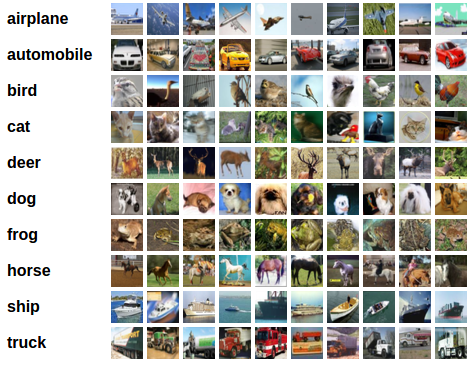
\includegraphics[width=0.72\linewidth]{figures/cifar10.png}
\caption[CIFAR-10 example images]{Example images from the CIFAR-10 dataset. CIFAR-10 contains ten object categories represented by low-resolution \(32 \times 32\) color images.}
\label{fig:ch5_cifar10_examples}
\end{figure}
Each image has spatial resolution \(32 \times 32\) with three color channels. The official dataset contains 50,000 training images and 10,000 test images. In our experimental pipeline, the original training split is partitioned into 40,000 images for training and 10,000 images for validation and checkpoint selection, while the official 10,000-image test split is reserved for final test-set evaluation.

The validation set is used only for model selection and hyperparameter monitoring. Final reported numbers are computed on the test set after the checkpoint has been selected. This separation is important because adversarial robustness estimates can vary across random seeds and training checkpoints; using a held-out validation set reduces the risk of selecting a checkpoint based on test-set performance.
All images are normalized using the same preprocessing pipeline across methods. During training, standard CIFAR-10 data augmentation is applied to the clean images before adversarial examples are generated. The augmentation includes random cropping with padding and random horizontal flipping. During validation and testing, no stochastic augmentation is used. This ensures that differences between methods are caused by the training objective rather than by differences in preprocessing or evaluation.

The same dataset split, preprocessing pipeline, and evaluation dataloaders are used for all compared methods. This includes the single-attack PGD-AT and DDN-AT baselines, Multi-AT, AttackDRO, Cluster-DRO, and AttackDRO++.

\section{Model Architecture}

The primary architecture used in this study is ResNet-18, based on the residual learning
framework of He et al.~\cite{he2016deep}, adapted for CIFAR-10 resolution. ResNet-18
provides a useful balance between expressiveness and computational cost: it is large
enough to support nontrivial adversarial training experiments, but still efficient enough
to run repeated-seed comparisons and ablation studies.

The classifier is denoted by \(f_\theta\). For an input image \(x\), the model outputs logits
$$
z = f_\theta(x) \in \mathbb{R}^{C},
$$
where \(C=10\) is the number of CIFAR-10 classes. In addition to logits, the proposed method requires access to the penultimate-layer representation
$$
h = \phi_\theta(x) \in \mathbb{R}^{d_h}.
$$

This feature vector is used for clustering adversarial examples in AttackDRO++ and for constructing the gradient-fingerprint augmented feature described in Chapter 4. For ResNet-18 on CIFAR-10, the penultimate representation dimension is \(d_h = 512\). Therefore, the raw classifier-head gradient proxy has dimension \(C d_h = 10 \times 512 = 5120\), which is later reduced by random projection.

Unless otherwise stated, all main experiments use the same ResNet-18 architecture and differ only in the training objective. This controlled setup ensures that performance differences can be attributed to the training method rather than to architectural changes. Higher-capacity architectures are treated as scaling checks or future extensions rather than the main basis for comparison.

\section{Attack Suite and Configuration}
% TODO[Kiệt]:
% Goal:
% - Make this section the source of truth for attack names and configurations.
% Flow:
% - Separate source/training attacks from evaluation-only attacks and AutoAttack.
% - Define PGD-$\ell_\infty$ once as the 20-step cross-entropy source attack.
% Include:
% - Ensure tables cover attack, norm, budget, steps, loss/objective, role, and whether used for training/evaluation.
% - Cite docs/05_notation_registry.md names in formal table/caption text.
% Avoid:
% - Repeating code-style names like `PGD20-CE` in prose.
% Target length: 4-6 paragraphs plus configuration tables.
Stage 2 evaluates whether robustness learned from a small set of source attacks generalizes to a broader attack suite. The attack suite is divided into two groups: source attacks used during training and evaluation attacks used only for validation or final testing.

\subsection{Training attacks}
The main training setup uses two source attacks:
\[
    \mathcal{A}_{\mathrm{src}}
    =
    \{\text{PGD-}\ell_\infty,\text{DDN-}\ell_2\}.
\]
PGD-\(\ell_\infty\) represents the standard first-order \(\ell_\infty\) adversarial
training setting. It uses cross-entropy loss and perturbation budget
\(\varepsilon_\infty = 8/255\). DDN-\(\ell_2\) is based on the Decoupled Direction and
Norm attack of Rony et al.~\cite{rony2019decoupling}. DDN is an efficient gradient-based
\(\ell_2\) attack that decouples the perturbation direction from its norm: the direction
is updated using gradient information, while the perturbation norm is adapted depending
on whether the current example is already adversarial.



Table~\ref{tab:training_attacks} summarizes the source attacks used during training.
Both attacks are used to generate mixed adversarial minibatches for Multi-ATtack
ERM, AttackDRO, AttackDRO++, and the proposed AttackDRO++ Anchor35 GradFP method.

\begin{table}[H]
\centering
\caption{Training attack configuration.}
\label{tab:training_attacks}
\begin{tabular}{llllll}
\toprule
Attack & Norm & Budget & Steps & Loss / objective & Role \\
\midrule
PGD-{$\ell_\infty$} & $\ell_\infty$ & $8/255$ & 20 & Cross-entropy & Source attack \\
DDN-$\ell_2$ & $\ell_2$ & $0.5$ & 20 & DDN objective & Source attack \\
\bottomrule
\end{tabular}
\end{table}

ForMulti-ATtack training, each minibatch is split across the source attacks and adversarial examples are generated using the assigned attack. The same mixed-batch source attack construction is also used by AttackDRO, AttackDRO++, and the proposed AttackDRO++ Anchor35 GradFP method. Thus, the compared methods share the same adversarial data generation process and differ mainly in how they weight or group the generated examples.

\subsection{Evaluation Attacks}
\label{sec:evaluation_attacks}

The evaluation suite includes both source attacks and held-out attacks. The two source
attacks used during training are also included in validation and test evaluation, while
the remaining attacks are held out from training. This protocol directly tests the
attacks-as-domains hypothesis: a robust model should not only perform well on the attacks
used for optimization, but should also generalize to attacks with different perturbation
geometries and optimization dynamics.


For validation and final testing, we evaluate each checkpoint using the attack suite in
Table~\ref{tab:evaluation_attacks}. The main aggregate metric, denoted Mean(8), is
computed over the eight attacks in the table. AutoAttack is reported separately and is
therefore not included in Mean(8).
\begin{table}[H]
\centering
\caption{Validation and test attacks used for Mean(8).}
\label{tab:evaluation_attacks}
\renewcommand{\arraystretch}{1.08}
\setlength{\tabcolsep}{7pt}
\begin{tabular}{lcccc}
\toprule
Attack & Norm & Budget & Steps & Group \\
\midrule
FGSM-RS              & $\ell_\infty$ & $8/255$ & 1   & Held-out $\ell_\infty$ \\
PGD-$\ell_\infty$   & $\ell_\infty$ & $8/255$ & 20  & Source \\
TPGD                 & $\ell_\infty$ & $8/255$ & 10  & Held-out $\ell_\infty$ \\
MI-FGSM              & $\ell_\infty$ & $8/255$ & 10  & Held-out $\ell_\infty$ \\
PGD-$\ell_2$         & $\ell_2$      & $0.5$   & 10  & Held-out $\ell_2$ \\
DDN-$\ell_2$         & $\ell_2$      & $0.5$   & 20  & Source \\
DeepFool-$\ell_2$    & $\ell_2$      & $0.5$   & 50  & Held-out $\ell_2$ \\
CW-$\ell_2$          & $\ell_2$      & $0.5$   & 200 & Held-out $\ell_2$ \\
\bottomrule
\end{tabular}
\end{table}

For aggregate analysis, we report four summary metrics derived from the same eight
attacks: Seen, Held-out \(\ell_\infty\), Held-out \(\ell_2\), and Mean(8). Their exact
definitions are given in Section~\ref{sec:evaluation_metrics}.

\paragraph{AutoAttack configuration}

AutoAttack is used as an additional standardized \(\ell_\infty\) stress test following
Croce and Hein~\cite{croce2020reliable}. It is not included in Mean(8), because it is
computationally more expensive and follows a separate evaluation protocol.

The AutoAttack configuration uses the standard \(\ell_\infty\) setting with perturbation
budget \(\varepsilon_\infty = 8/255\). In early experiments and ablations, AutoAttack is
sometimes evaluated on a subset of 512 test samples as a sanity check. These 512-sample
results are useful for detecting severe robustness collapse, but they are not used as the
primary ranking criterion because the sample size is smaller and the variance is higher.
For the final stress test, AutoAttack is evaluated on the full test set for selected
representative seeds.

\begin{table}[H]
\centering
\caption{AutoAttack configuration.}
\label{tab:autoattack_config}
\renewcommand{\arraystretch}{1.08}
\setlength{\tabcolsep}{10pt}
\begin{tabular}{lccc}
\toprule
Attack & Norm & Budget & Role \\
\midrule
AutoAttack & $\ell_\infty$ & $8/255$ & Separate stress test \\
\bottomrule
\end{tabular}
\end{table}

\section{Training Configuration}

All methods are trained under a controlled adversarial training pipeline. Unless
otherwise stated, the optimizer, model architecture, dataset split, preprocessing
pipeline, and evaluation protocol are kept fixed across methods. This ensures that
performance differences mainly come from the training objective rather than from
implementation or evaluation differences.

To make method differences attributable to the training objective, Table~\ref{tab:ch5_training_config}
fixes the shared training configuration for the main experiments. All main experiments use ResNet-18 on CIFAR-10 with stochastic gradient descent (SGD),
momentum, weight decay, mixed-precision training, and a multi-step learning-rate
schedule. The main methods are trained for 50 epochs. During training, each minibatch
contains a balanced mixture of source attacks. In the two-source setting, approximately
half of the minibatch is assigned to PGD-\(\ell_\infty\) and the other half to
DDN-\(\ell_2\).

\begin{table}[H]
\centering
\caption{General training configuration used for the main experiments.}
\label{tab:ch5_training_config}
\footnotesize
\setlength{\tabcolsep}{4pt}
\renewcommand{\arraystretch}{1.08}
\begin{tabularx}{\textwidth}{@{}
>{\raggedright\arraybackslash}p{0.25\textwidth}
>{\raggedright\arraybackslash}p{0.22\textwidth}
>{\raggedright\arraybackslash}X
@{}}
\toprule
Component & Setting & Description \\
\midrule
Dataset & CIFAR-10 & 40k train / 10k validation / 10k test. \\
Backbone & ResNet-18 & CIFAR-10 adapted residual network. \\
Training epochs & 50 & Main training budget. \\
Batch size & 128 & Used for all main methods. \\
Optimizer & SGD & Momentum-based stochastic gradient descent. \\
Momentum & 0.9 & Standard SGD momentum. \\
Weight decay & $5 \times 10^{-4}$ & Weight regularization. \\
Initial learning rate & 0.1 & Decayed during training. \\
Learning-rate schedule & Multi-step & Same schedule for all compared methods. \\
Mixed precision & Enabled & Reduces memory usage and training time. \\
Gradient clipping & Enabled & Stabilizes adversarial training. \\
Checkpoint selection & Validation robust average & Test set is used only after selection. \\
\bottomrule
\end{tabularx}
\end{table}

Checkpoint selection is based on validation robustness rather than test performance.
After training, the selected checkpoint is evaluated once on the test set. This protocol
is applied consistently to the uniform baseline and all AttackDRO variants.

The method overview in Table~\ref{tab:ch5_method_training_summary} separates each
training objective by its grouping or weighting strategy. All multi-attack methods use
the same source attacks and mixed-batch adversarial example generation; they differ only
in how adversarial examples are weighted or grouped during optimization.

\begin{table}[H]
\centering
\caption{Training methods compared in the CIFAR-10 and ResNet-18 experiments.}
\label{tab:ch5_method_training_summary}
\footnotesize
\setlength{\tabcolsep}{4pt}
\renewcommand{\arraystretch}{1.08}
\begin{tabularx}{\textwidth}{@{}
>{\raggedright\arraybackslash}p{0.24\textwidth}
>{\raggedright\arraybackslash}p{0.34\textwidth}
>{\raggedright\arraybackslash}X
@{}}
\toprule
Method & Grouping / weighting strategy & Experimental role \\
\midrule
PGD-AT
& One source attack only
& Specialist $\ell_\infty$ baseline. \\

DDN-AT
& One source attack only
& Specialist $\ell_2$ baseline. \\

Multi-AT
& Uniform sample weighting over mixed PGD-$\ell_\infty$ and DDN-$\ell_2$ batches
& Main strong baseline. \\

AttackDRO
& Group DRO over attack identity
& Coarse attack-level DRO baseline. \\

Cluster-DRO
& Group DRO over discovered clusters
& Intermediate cluster-level grouping baseline. \\

AttackDRO++
& Uniform-anchored Cluster-DRO with gradient fingerprints
& Proposed final method. \\
\bottomrule
\end{tabularx}
\end{table}

For the proposed method, cluster assignments are refreshed periodically using a feature
bank. The default refresh interval is two epochs. The cluster weight vector
\(\mathbf{q}\) is updated only after a warmup period, so that early noisy representations
do not dominate adaptive reweighting.

% ─────────────────────────────────────────────────────────────────────────────
\section{Hyperparameter Choices and Ablation Factors}
\label{sec:hyperparameters}

% TODO[Kiệt]:
% Goal:
% - Explain why default hyperparameters and ablation factors were chosen.
% Flow:
% - Default configuration first, then ablation dimensions and what each tests.
% Include:
% - Keep values synchronized with Chapter 4 `tab:hparams` and Chapter 6 ablation tables.
% Avoid:
% - Reporting ablation outcomes in this setup chapter.
% Target length: 4-6 paragraphs plus existing tables.
% ─────────────────────────────────────────────────────────────────────────────

\begin{table}[H]
\centering
\caption{Default hyperparameters for AttackDRO++ (Ours).}
\label{tab:main_hyperparams}
\footnotesize
\setlength{\tabcolsep}{3.5pt}
\renewcommand{\arraystretch}{1.05}
\begin{tabularx}{\textwidth}{@{}
>{\raggedright\arraybackslash}p{0.25\textwidth}
>{\centering\arraybackslash}p{0.14\textwidth}
>{\raggedright\arraybackslash}p{0.22\textwidth}
>{\raggedright\arraybackslash}X
@{}}
\toprule
Hyperparameter & Symbol & Default value & Purpose \\
\midrule

Source attacks
& $\mathcal{A}_{\mathrm{src}}$
& PGD-20$_{\mathrm{CE}}$, DDN-$\ell_2$
& Training attack domains. \\

Number of clusters
& $K$
& 4
& Latent group granularity. \\

DRO anchor strength
& $\lambda_{\mathrm{DRO}}$
& 0.35
& Balances ERM and Cluster-DRO. \\

$q$ learning rate
& $\eta_q$
& $3 \times 10^{-4}$
& Step size for $q$ update. \\

$q$ floor
& $q_{\min}$
& 0.03
& Prevents ignored clusters. \\

$q$ warmup
& $T_w$
& 3 epochs
& Delays early reweighting. \\

Cluster refresh interval
& $R$
& 2 epochs
& K-means refresh frequency. \\

Feature bank size
& $|\mathcal{F}|$
& 4096
& Stores detached features. \\

Gradient projection dim.
& $d_{\mathrm{proj}}$
& 128
& Compresses GradFP features. \\

Gradient feature weight
& $\lambda_{\mathrm{grad}}$
& 0.1
& Weights GradFP features. \\

Label feature weight
& $\lambda_{\mathrm{lbl}}$
& 0.1
& Weights label features. \\

Clusterer
& --
& K-means
& Assigns latent groups. \\

$q$ refresh policy
& --
& Reset after refresh
& Avoids stale cluster weights. \\

\bottomrule
\end{tabularx}
\end{table}

The number of clusters is set to $K=4$ as a moderate grouping resolution. Too few
clusters may fail to capture meaningful difficulty structure, while too many clusters may
fragment the minibatch and produce noisy group-loss estimates. The default anchor
strength $\lambda_{\mathrm{DRO}}=0.35$ is chosen to keep theMulti-ATtack loss as
the dominant stabilizing signal while still allowing cluster-level adaptive correction.

The $q$-floor and warmup settings are included for stability. The floor projection
prevents any cluster from being completely ignored, while the warmup period prevents the
exponentiated-gradient update from acting on unreliable early cluster assignments. The
feature bank and refresh interval control how quickly the clusterer adapts to evolving
model representations. In the default setting, refreshing every two epochs provides a
balance between stability and adaptivity.

The gradient fingerprint is projected to $d_{\mathrm{proj}}=128$ dimensions for
computational efficiency. For CIFAR-10 with ResNet-18, the classifier-head gradient proxy
has raw dimension $C d_h = 10 \times 512 = 5120$. The fixed random projection reduces
this dimension while retaining useful information about the optimization direction
induced by each adversarial example.

Table~\ref{tab:ablation_hyperparams} lists the main hyperparameters varied in ablation
experiments. These ablations are used in Chapter~6 to justify the default configuration
and to separate the effect of the proposed components from the strong uniform
multi-attack baseline.

\begin{table}[H]
\centering
\caption{Hyperparameters varied in ablation studies.}
\label{tab:ablation_hyperparams}
\footnotesize
\setlength{\tabcolsep}{4pt}
\renewcommand{\arraystretch}{1.08}
\begin{tabularx}{\textwidth}{@{}
>{\raggedright\arraybackslash}p{0.25\textwidth}
>{\raggedright\arraybackslash}p{0.32\textwidth}
>{\raggedright\arraybackslash}X
@{}}
\toprule
Ablation factor & Values / variants & Purpose \\
\midrule

Anchor strength
& $\lambda_{\mathrm{DRO}} \in \{0.20, 0.35, 0.50\}$
& Tests the uniform-anchor trade-off. \\

Cluster count
& $K \in \{2,4,6,10\}$
& Tests sensitivity to group granularity. \\

$q$ update
& update $q$  vs. uniform $q$
& Tests adaptive reweighting. \\

Refresh schedule
& 1 epoch vs. 2 epochs
& Tests cluster-refresh frequency. \\

Gradient fingerprint
& With vs. without GradFP
& Tests optimization-level features. \\

Random clusters
& Learned vs. random assignment
& Negative control for clustering. \\

\bottomrule
\end{tabularx}
\end{table}

\section{Statistical Significance Protocol}
\label{sec:statistical-significance-protocol}

To ensure that the reported improvements are not caused by seed-specific randomness, this study applies a repeated-seed statistical protocol. Each method is trained and evaluated under the same set of seeds, dataset split, architecture, attack suite, and evaluation configuration. The seed-level result is used as the basic unit of analysis.

For a given metric, let $x_i$ be the performance of AttackDRO++ under seed $i$, and let $y_i$ be the performance of a baseline method under the same seed. The paired difference is defined as:

\begin{equation}
    d_i = x_i - y_i.
\end{equation}

All statistical comparisons are performed on these paired differences. This paired design reduces the influence of random initialization, data shuffling, and optimization noise, allowing the analysis to focus on the relative performance difference between methods.

The primary significance test is the Wilcoxon signed-rank test. This test is selected because it is non-parametric and does not assume that the paired differences are normally distributed. This property is important for repeated-seed adversarial robustness experiments, where the number of seeds is limited and the distribution of performance differences may be irregular. For directional comparisons, the alternative hypothesis is that AttackDRO++ achieves higher performance than the baseline:

\begin{align}
    H_0 &: \operatorname{median}(d_i) \leq 0, \\
    H_1 &: \operatorname{median}(d_i) > 0.
\end{align}

A paired $t$-test is also reported as a secondary parametric check. While the paired $t$-test assumes approximate normality of the paired differences, it provides a useful sanity check. When both the Wilcoxon signed-rank test and the paired $t$-test support the same conclusion, the result is considered more stable. If the two tests disagree, the Wilcoxon test is prioritized because it is less dependent on distributional assumptions.

In addition to $p$-values, this study reports the paired effect size using Cohen's $d_z$:

\begin{equation}
    d_z = \frac{\bar{d}}{s_d},
\end{equation}

where $\bar{d}$ is the mean paired difference and $s_d$ is the sample standard deviation of the paired differences. Cohen's $d_z$ is used to quantify the magnitude of the improvement. Conventional thresholds are used as rough guidance, with $0.2$, $0.5$, and $0.8$ corresponding to small, medium, and large effects, respectively. However, in adversarial robustness evaluation, even moderate effect sizes may be practically meaningful if the improvement is consistent across strong attacks or improves worst-case robustness.

To estimate uncertainty, 95\% bootstrap confidence intervals are computed from seed-level results. For each method and metric, the seed-level values are resampled with replacement 10{,}000 times, and the mean is recomputed for each resample. The 2.5th and 97.5th percentiles of the bootstrap distribution are used as the confidence interval. Bootstrap confidence intervals are also computed for the paired difference $x_i - y_i$, as this directly estimates the uncertainty of the improvement over each baseline.

Because multiple attacks, metrics, and baseline comparisons are evaluated, Holm--Bonferroni correction is applied within each metric family. Both raw and corrected $p$-values are reported, but corrected $p$-values are used for final significance interpretation. This correction reduces the risk of false positive findings while remaining less conservative than the standard Bonferroni correction.

The reporting format used in the results chapter is summarized in Table~\ref{tab:statistical-reporting-format}.

\begin{table}[H]
\centering
\caption{Reporting format for the statistical significance protocol.}
\label{tab:statistical-reporting-format}
\footnotesize
\setlength{\tabcolsep}{4pt}
\renewcommand{\arraystretch}{1.08}
\begin{tabularx}{\textwidth}{@{}
>{\raggedright\arraybackslash}p{0.26\textwidth}
>{\raggedright\arraybackslash}p{0.30\textwidth}
>{\raggedright\arraybackslash}X
@{}}
\toprule
Quantity & Reported value & Purpose \\
\midrule

Mean performance
& Mean across seeds
& Reports average robustness. \\

Seed variation
& Standard deviation
& Measures run-to-run variability. \\

Uncertainty
& 95\% bootstrap confidence interval
& Estimates uncertainty of the mean. \\

Primary test
& Wilcoxon signed-rank test
& Non-parametric paired comparison. \\

Secondary test
& Paired $t$-test
& Parametric sanity check. \\

Effect size
& Cohen's $d_z$
& Measures magnitude of improvement. \\

Correction
& Holm--Bonferroni correction
& Controls multiple comparisons. \\

\bottomrule
\end{tabularx}
\end{table}

A comparison is considered statistically supported when AttackDRO++ improves the mean metric, obtains a corrected $p$-value below the significance threshold, and shows a non-trivial paired effect size. This protocol is applied consistently to white-box robustness, gray-box transfer robustness, aggregate robustness metrics, and ablation studies.

% ─────────────────────────────────────────────────────────────────────────────
\section{Evaluation Metrics and Robustness Definitions}
\label{sec:evaluation_metrics}

% TODO[Kiệt]:
% Goal:
% - Define every metric used in Chapter 6 before result interpretation begins.
% Flow:
% - Clean accuracy, per-attack robust accuracy, Mean(8), Worst(8), seen/held-out groups, AutoAttack, graybox accuracy, and per-class/per-attack accuracy.
% Include:
% - State which metrics are allowed as shorthand after definition.
% - Keep equation labels only for metrics referenced later.
% Avoid:
% - Using metric shorthand in section titles.
% Target length: 5-7 paragraphs plus metric summary table.
% ─────────────────────────────────────────────────────────────────────────────

This section defines the metrics used to compare all methods. Let
\[
    \mathcal{D}_{\mathrm{test}}
    =
    \{(\mathbf{x}_i, y_i)\}_{i=1}^{n}
\]
denote the test set, and let \(A\) be an adversarial attack. The adversarial example
generated by \(A\) is denoted by
\[
    \mathbf{x}_i^{A} = A(f_\theta, \mathbf{x}_i, y_i).
\]
The robust accuracy under attack \(A\) is
\begin{equation}
    \mathrm{Acc}(A)
    =
    \frac{1}{n}
    \sum_{i=1}^{n}
    \mathbb{I}
    \left[
        \arg\max_c f_\theta(\mathbf{x}_i^{A})_c = y_i
    \right].
    \label{eq:attack_acc}
\end{equation}

Clean accuracy is computed without adversarial perturbation:
\begin{equation}
    \mathrm{Acc}_{\mathrm{clean}}
    =
    \frac{1}{n}
    \sum_{i=1}^{n}
    \mathbb{I}
    \left[
        \arg\max_c f_\theta(\mathbf{x}_i)_c = y_i
    \right].
\end{equation}

The primary aggregate metric is Mean(8), defined as the average robust accuracy over the
eight non-AutoAttack evaluation attacks:
\begin{equation}
    \mathrm{Mean}(8)
    =
    \frac{1}{|\mathcal{A}_{8}|}
    \sum_{A \in \mathcal{A}_{8}}
    \mathrm{Acc}(A),
    \label{eq:mean8}
\end{equation}
where
\[
\mathcal{A}_{8}
=
\{
\text{FGSM-RS},
\text{PGD-}\ell_\infty,
\text{TPGD},
\text{MI-FGSM},
\text{PGD-}\ell_2,
\text{DDN-}\ell_2,
\text{DeepFool-}\ell_2,
\text{CW-}\ell_2
\}.
\]

We also report the worst robust accuracy across the same eight attacks:
\begin{equation}
    \mathrm{Worst}(8)
    =
    \min_{A \in \mathcal{A}_{8}}
    \mathrm{Acc}(A).
    \label{eq:worst8}
\end{equation}

For finer analysis, we report seen, held-out \(\ell_\infty\), and held-out \(\ell_2\)
averages:
\begin{align}
    \mathrm{Seen}
    &=
    \frac{1}{2}
    \left[
        \mathrm{Acc}(\text{PGD-}\ell_\infty)
        +
        \mathrm{Acc}(\text{DDN-}\ell_2)
    \right], \\
    \mathrm{Heldout}_{\ell_\infty}
    &=
    \frac{1}{3}
    \left[
        \mathrm{Acc}(\text{FGSM-RS})
        +
        \mathrm{Acc}(\text{TPGD})
        +
        \mathrm{Acc}(\text{MI-FGSM})
    \right], \\
    \mathrm{Heldout}_{\ell_2}
    &=
    \frac{1}{3}
    \left[
        \mathrm{Acc}(\text{PGD-}\ell_2)
        +
        \mathrm{Acc}(\text{DeepFool-}\ell_2)
        +
        \mathrm{Acc}(\text{CW-}\ell_2)
    \right].
\end{align}

AutoAttack is reported separately from Mean(8). Early ablations may use AutoAttack on
512 test samples as a sanity check, while final AutoAttack comparisons are reported on
the full test set for selected representative seeds.

For graybox evaluation, adversarial examples are generated using a surrogate model
\(f_{\theta_s}\) and evaluated on a target model \(f_{\theta_t}\):
\begin{equation}
    \mathrm{Acc}_{s \rightarrow t}(A)
    =
    \frac{1}{n}
    \sum_{i=1}^{n}
    \mathbb{I}
    \left[
        \arg\max_c f_{\theta_t}
        \left(
            A(f_{\theta_s}, \mathbf{x}_i, y_i)
        \right)_c
        =
        y_i
    \right].
    \label{eq:graybox_acc}
\end{equation}
Thus, the same table supports whitebox, same-method transfer, and cross-method graybox
evaluation.

Finally, for fine-grained analysis, each attack-class pair is treated as an evaluation
group. For attack \(A\) and class \(c\), the attack-class group accuracy is
\begin{equation}
    \mathrm{Acc}(A,c)
    =
    \frac{1}{|\mathcal{D}_{c}|}
    \sum_{(\mathbf{x}_i,y_i)\in \mathcal{D}_{c}}
    \mathbb{I}
    \left[
        \arg\max_j f_\theta(\mathbf{x}_i^{A})_j = y_i
    \right],
    \label{eq:attack_class_acc}
\end{equation}
where \(\mathcal{D}_{c}\) is the subset of test examples whose label is \(c\).

\begin{table}[H]
\centering
\caption{Summary of evaluation metrics.}
\label{tab:evaluation_metrics_summary}
\footnotesize
\setlength{\tabcolsep}{4pt}
\renewcommand{\arraystretch}{1.08}
\begin{tabularx}{\textwidth}{@{}
>{\raggedright\arraybackslash}p{0.24\textwidth}
>{\raggedright\arraybackslash}p{0.34\textwidth}
>{\raggedright\arraybackslash}X
@{}}
\toprule
Metric & Definition & Purpose \\
\midrule
Clean accuracy
& Accuracy on unperturbed test images
& Measures standard classification performance. \\

Per-attack robust accuracy
& Accuracy under a single adversarial attack
& Shows which attacks each method resists or fails against. \\

Mean(8)
& Average accuracy over the eight non-AutoAttack attacks
& Main aggregate robustness metric. \\

Worst(8)
& Minimum accuracy over the eight non-AutoAttack attacks
& Measures the weakest attack in the suite. \\

Seen mean
& Average over PGD-$\ell_\infty$ and DDN-$\ell_2$
& Measures robustness on source attacks. \\

Held-out $\ell_\infty$ mean
& Average over FGSM-RS, TPGD, and MI-FGSM
& Measures transfer to unseen $\ell_\infty$ attacks. \\

Held-out $\ell_2$ mean
& Average over PGD-$\ell_2$, DeepFool-$\ell_2$, and CW-$\ell_2$
& Measures transfer to unseen $\ell_2$ attacks. \\

AutoAttack
& Standard $\ell_\infty$ AutoAttack robust accuracy
& Separate robustness stress test. \\

Graybox transfer accuracy
& Target accuracy on adversarial examples generated by a surrogate
& Measures transfer robustness across models. \\

Attack-class group accuracy
& Accuracy for each attack $\times$ class pair
& Diagnoses fine-grained failure modes. \\
\bottomrule
\end{tabularx}
\end{table}

% ─────────────────────────────────────────────────────────────────────────────
\section{Graybox Transfer Protocol}
\label{sec:graybox-design}
% ─────────────────────────────────────────────────────────────────────────────

To evaluate whether the proposed method changes the structure of learned robustness
rather than only improving whitebox accuracy, we conduct a cross-model graybox transfer
experiment. The experiment uses four method families: PGD-AT,
DDN-AT, Multi-AT, and AttackDRO++ (Ours).
Each method is evaluated over five representative seeds, giving 20 checkpoints in total.

Each checkpoint is used in two roles. As a \emph{surrogate}, it generates adversarial
examples. As a \emph{target}, it is evaluated on adversarial examples generated by all
surrogate checkpoints. Therefore, the full protocol evaluates
\[
    20 \times 20 = 400
\]
surrogate--target pairs. This design produces whitebox, same-method transfer, and
cross-method graybox transfer results from a single unified evaluation table.

To keep the computation tractable while still supporting per-class and per-attack
analysis, each surrogate checkpoint generates a balanced adversarial cache. The CIFAR-10
test set contains 1000 images per class. For each class, the test images are split evenly
across the eight evaluation attacks. Thus, each attack-class cell contains 125 source
images:
\[
    10 \text{ classes}
    \times
    8 \text{ attacks}
    \times
    125 \text{ examples}
    =
    10{,}000
\]
adversarial examples per surrogate checkpoint.

The class-wise split is generated deterministically using a fixed shuffle seed. Therefore,
the same attack-class cell always refers to the same underlying CIFAR-10 source images
across surrogate checkpoints. This makes paired comparisons between surrogate and
target methods well aligned.

For each surrogate--target pair, the evaluation produces one row per attack-class group,
indexed by surrogate method, surrogate seed, target method, target seed, attack, and
class. Since there are 80 attack-class groups per pair, the full table contains
\(400 \times 80 = 32{,}000\) rows. Transfer matrices, attack-class drilldowns, and
paired method comparisons are all computed by aggregating this same long-form table. Table~\ref{tab:graybox_transfer_regimes} summarizes the transfer regimes used in the
analysis.

\begin{table}[H]
\centering
\caption{Transfer regimes in the graybox evaluation protocol.}
\label{tab:graybox_transfer_regimes}
\footnotesize
\setlength{\tabcolsep}{4pt}
\renewcommand{\arraystretch}{1.08}
\begin{tabularx}{\textwidth}{@{}
>{\raggedright\arraybackslash}p{0.25\textwidth}
>{\raggedright\arraybackslash}p{0.25\textwidth}
>{\raggedright\arraybackslash}p{0.17\textwidth}
>{\raggedright\arraybackslash}X
@{}}
\toprule
Regime & Condition & Rows & Purpose \\
\midrule

Whitebox
& Same method and same seed
& $20 \times 80 = 1{,}600$
& Recovers standard whitebox robustness as a sanity check. \\

Same-method transfer
& Same method, different seed
& $80 \times 80 = 6{,}400$
& Measures seed-to-seed transfer within a method family. \\

Cross-method same-seed
& Different methods, same seed
& $60 \times 80 = 4{,}800$
& Measures transfer between method families under matched seeds. \\

Cross-method cross-seed
& Different methods, different seeds
& $240 \times 80 = 19{,}200$
& Measures the most general cross-method graybox transfer setting. \\

\bottomrule
\end{tabularx}
\end{table}

In Chapter~6, the cross-method same-seed and cross-method cross-seed regimes are
combined to form the main graybox transfer analysis. The whitebox and same-method
transfer regimes are reported separately as diagnostic checks.

% ─────────────────────────────────────────────────────────────────────────────
\section{Tools, Platforms, and Experiment Tracking}
\label{sec:ch5_tools_platforms}
% ─────────────────────────────────────────────────────────────────────────────

The experiments in this report were implemented in Python using a PyTorch-based
training pipeline. The codebase is organized around a configurable experiment
script that defines dataset construction, model initialization, adversarial attack
generation, training objectives, checkpoint selection, and fixed
evaluation scripts in one place. This organization is important because the compared methods differ
mainly in their grouping and weighting strategies, while the dataset split,
architecture, source attacks, evaluation attacks, optimizer, and checkpointing
rules are kept fixed.

Because reproducibility depends on both the training code and the analysis stack,
Table~\ref{tab:ch5_tools_platforms} records the tools and platforms that form the
experimental workflow. Google Colab and Google Drive are used for
interactive execution and persistent storage of checkpoints, cached adversarial
examples, figures, and result files. PyTorch and torchvision provide the core
deep-learning infrastructure, including model definitions, data loading, and
optimization. The attack implementations are built primarily with TorchAttacks,
with AutoAttack-$\ell_\infty$ and DDN-$\ell_2$ handled through their dedicated
packages when required. scikit-learn is used for K-means clustering in
AttackDRO++, while NumPy and pandas are used to aggregate seed-level and
attack-level results.

\begin{table}[H]
\centering
\caption{Tools and platforms used in the experimental workflow. The table lists only tools that are part of the implemented training, evaluation, logging, or reporting pipeline.}
\label{tab:ch5_tools_platforms}
\footnotesize
\setlength{\tabcolsep}{4pt}
\renewcommand{\arraystretch}{1.08}
\begin{tabularx}{\textwidth}{@{}
>{\raggedright\arraybackslash}p{0.24\textwidth}
>{\raggedright\arraybackslash}p{0.28\textwidth}
>{\raggedright\arraybackslash}X
@{}}
\toprule
Tool / platform & Role & Use in this report \\
\midrule

Google Colab
& Interactive execution environment
& Used to run training and evaluation notebooks with GPU support. \\

Google Drive
& Persistent experiment storage
& Stores checkpoints, cached adversarial examples, result tables, figures, and intermediate analysis files. \\

Python
& Main implementation language
& Used for the full training, evaluation, analysis, and plotting pipeline. \\

PyTorch
& Deep-learning framework
& Implements model training, automatic differentiation, mixed-precision execution, and checkpoint loading. \\

torchvision
& Dataset and model utilities
& Provides CIFAR-10 loading, image transforms, and ResNet backbones adapted for small images. \\

TorchAttacks
& Adversarial attack library
& Provides most gradient-based and optimization-based attacks used in training and evaluation. \\

AutoAttack package
& Standardized robustness stress test
& Used for AutoAttack-$\ell_\infty$ evaluation with perturbation budget $8/255$. \\

adv-lib
& DDN attack implementation
& Used for DDN-$\ell_2$ adversarial example generation. \\

scikit-learn
& Clustering utilities
& Provides MiniBatch K-means for cluster discovery in AttackDRO++. \\

NumPy and pandas
& Result processing
& Used to aggregate per-seed, per-attack, per-class, and graybox transfer results. \\

matplotlib and SciencePlots
& Visualization
& Used to generate plots and publication-style figures for analysis. \\

Weights \& Biases
& Experiment tracking
& Logs configurations, training curves, validation metrics, group weights, and diagnostic figures when enabled. \\

\bottomrule
\end{tabularx}
\end{table}

Experiment tracking is treated as part of the reproducibility protocol rather than
as a separate result source. Each run records the method name, seed, dataset,
backbone, source attacks, evaluation attacks, and key hyperparameters. During
training, the pipeline logs loss, adversarial accuracy, validation robustness,
learning rate, checkpoint state, and group-weight diagnostics when applicable.
Representative Weights \& Biases (W\&B) tracking exports are provided in
Appendix~\ref{app:logs}.

All test-set claims in Chapter~6 are based on saved checkpoints that are loaded
after training and evaluated using fixed evaluation scripts. The main result
tables are produced from structured result files rather than from manually copied
console logs. This separation reduces the risk of mixing validation, test, whitebox, graybox, and diagnostic metrics. It
also makes it possible to reuse the same result files for aggregate metrics,
per-attack analysis, per-class analysis, and paired statistical comparisons.

\paragraph{Summary.}
The setup summary in Table~\ref{tab:ch5_setup_summary} serves as the reproducibility
contract for the result claims in Chapter~6 by collecting the dataset, model, attack
suite, repeated-seed protocol, and analysis stack in one place.

\begin{table}[H]
\centering
\caption{Summary of the experimental setup used in this report. Unless otherwise stated, evaluations use CIFAR-10, ResNet-18, and the eight non-AutoAttack attacks for Mean(8), with AutoAttack-$\ell_\infty$ reported separately.}
\label{tab:ch5_setup_summary}
\footnotesize
\setlength{\tabcolsep}{4pt}
\renewcommand{\arraystretch}{1.08}
\begin{tabularx}{\textwidth}{@{}
>{\raggedright\arraybackslash}p{0.28\textwidth}
>{\raggedright\arraybackslash}X
@{}}
\toprule
Component & Configuration \\
\midrule

Dataset
& CIFAR-10 with 40{,}000 training images, 10{,}000 validation images, and 10{,}000 test images. \\

Backbone
& ResNet-18 adapted for CIFAR-10 resolution. \\

Main Chapter~6 compared methods
& PGD-AT, DDN-AT, Multi-AT, and AttackDRO++; AttackDRO and Cluster-DRO are intermediate design steps described in Chapter~\ref{chap:methodology}. \\

Source attacks
& PGD-$\ell_\infty$ and DDN-$\ell_2$. \\

Evaluation attacks for Mean(8)
& FGSM-RS, PGD-$\ell_\infty$, TPGD, MI-FGSM, PGD-$\ell_2$, DDN-$\ell_2$, DeepFool-$\ell_2$, and CW-$\ell_2$. \\

Separate stress test
& AutoAttack-$\ell_\infty$, reported separately from Mean(8). \\

Primary aggregate metric
& Mean(8): mean robust accuracy over the eight non-AutoAttack evaluation attacks. \\

Secondary metrics
& Worst(8), seen-source robustness, held-out $\ell_\infty$ robustness, held-out $\ell_2$ robustness, per-attack accuracy, per-class accuracy, and graybox transfer accuracy. \\

Repeated-seed protocol
& Aggregate whitebox tables use paired random-seed comparisons; class-wise and graybox panels use five random seeds per method. \\

Graybox protocol
& Four method families are evaluated across five random seeds each, giving 20 random-seed checkpoints and 400 surrogate--target pairs. \\

Statistical analysis
& Paired random-seed comparisons with Wilcoxon signed-rank tests, paired $t$-tests, bootstrap confidence intervals, effect sizes, and Holm--Bonferroni correction. \\

Implementation stack
& PyTorch, torchvision, TorchAttacks, AutoAttack package, adv-lib, scikit-learn, NumPy, pandas, matplotlib, SciencePlots, W\&B, Google Colab, and Google Drive. \\

\bottomrule
\end{tabularx}
\end{table}

This chapter has defined the experimental setting used throughout the remainder of
the report: the dataset, model, attacks, training configurations, hyperparameters,
statistical protocol, evaluation metrics, graybox transfer design, and
implementation tools. These definitions provide the reproducibility contract for
the empirical claims that follow. Chapter~\ref{chap:results_analysis} now presents the results obtained under this protocol and analyzes how the proposed method behaves under whitebox, graybox, per-class, and ablation settings.



\chapter{Results and Analysis}
\label{chap:results_analysis}
This chapter evaluates AttackDRO++ under the experimental protocol defined in
Chapter~\ref{chap:experimental_setup}. The main comparison includes four
methods: PGD-AT, DDN-AT, Multi-AT, and AttackDRO++. Multi-AT serves as the
primary strong baseline because it trains on both source attacks, whereas PGD-AT
and DDN-AT serve as single-attack specialists that reveal how robustness can
concentrate around one perturbation family.

The main aggregate metric, Mean(8), averages robust accuracy over eight
non-AutoAttack attacks: FGSM-RS, PGD-\(\ell_\infty\), TPGD, MI-FGSM,
PGD-\(\ell_2\), DDN-\(\ell_2\), DeepFool-\(\ell_2\), and CW-\(\ell_2\).
Among these attacks, PGD-\(\ell_\infty\) and DDN-\(\ell_2\) are the seen source
attacks used during training, while the remaining six attacks are held out from
optimization. Worst(8) reports the lowest robust accuracy among the same eight
attacks, and AutoAttack-\(\ell_\infty\) is reported separately as a standardized
stress check rather than as part of Mean(8).

The analysis proceeds from aggregate whitebox robustness to more targeted
diagnostics, including per-attack behavior, hardest-case checks, seed-to-seed
variation, class-wise patterns, graybox transfer, ablations, and supplementary
checks. The interpretation remains bounded: the goal is not to show universal
robustness or dominance under every attack, but to test whether latent cluster
reweighting, gradient fingerprints, and the uniform anchor provide a modest
refinement of uniform multi-attack training under the CIFAR-10 and ResNet-18
setting. Graybox significance tests are interpreted as transfer-trend evidence
rather than fully independent training-run proof.
% ─────────────────────────────────────────────────────────────────────────────
\section{Whitebox Robustness Under Direct Attacks}
\label{sec:ch6_whitebox}

\subsection{Aggregate Comparison Across Methods}
\label{subsec:ch6_aggregate_comparison}

\begin{table}[H]
\centering
\caption[Aggregate robust accuracy on the CIFAR-10 evaluation suite]{Aggregate robust accuracy (\%) on the CIFAR-10 evaluation suite,
reported as mean $\pm$ standard deviation across 20 random-seed runs.
Mean(8) is the average robust accuracy over the
eight non-AutoAttack evaluation attacks. Worst(8) is the lowest robust accuracy
among those same eight attacks. The
held-out attack mean averages FGSM-RS, TPGD, MI-FGSM, PGD-$\ell_2$,
DeepFool-$\ell_2$, and CW-$\ell_2$. The held-out $\ell_\infty$ mean averages
FGSM-RS, TPGD, and MI-FGSM; the held-out $\ell_2$ mean averages PGD-$\ell_2$,
DeepFool-$\ell_2$, and CW-$\ell_2$. The seen-source mean averages
PGD-$\ell_\infty$ and DDN-$\ell_2$. AutoAttack is reported separately and is
not included in Mean(8). Bold values indicate the best method for each metric.}
\label{tab:ch6_aggregate_results}
\footnotesize
\setlength{\tabcolsep}{1.25pt}
\renewcommand{\arraystretch}{1.08}
\begin{tabular}{@{}lcccc@{}}
\toprule
Metric & PGD-AT & DDN-AT & Multi-AT & AttackDRO++ (Ours) \\
\midrule
Mean(8)
& $60.499 \pm 0.327$
& $56.226 \pm 0.233$
& $62.045 \pm 0.447$
& \bestval{62.324 $\pm$ 0.147} \\

Held-out attack mean
& $62.268 \pm 0.390$
& $59.628 \pm 0.254$
& $64.083 \pm 0.505$
& \bestval{64.401 $\pm$ 0.155} \\

\hspace{1em}Held-out $\ell_\infty$ mean
& \bestval{62.515 $\pm$ 0.334}
& $51.594 \pm 0.306$
& $60.916 \pm 0.427$
& $61.149 \pm 0.170$ \\

\hspace{1em}Held-out $\ell_2$ mean
& $62.021 \pm 0.474$
& \bestval{67.661 $\pm$ 0.278}
& $67.249 \pm 0.603$
& $67.654 \pm 0.223$ \\

Seen-source mean
& $55.192 \pm 0.182$
& $46.020 \pm 0.247$
& $55.934 \pm 0.303$
& \bestval{56.093 $\pm$ 0.166} \\

\midrule
Worst(8)
& \bestval{49.656 $\pm$ 0.161}
& $25.957 \pm 0.378$
& $45.082 \pm 0.281$
& $45.079 \pm 0.237$ \\
\bottomrule



\end{tabular}
\end{table}
We compare four methods on 20 paired random-seed runs: PGD-AT,
DDN-AT, Multi-AT, and AttackDRO++ (Ours).
AttackDRO++ improves Mean(8) over Multi-AT by $+0.279$~pp ($p = 0.0076$,
14/20 wins), with the strongest channel on the held-out $\ell_2$ mean ($+0.405$~pp,
$p = 0.0079$, 16/20). It improves Mean(8) over PGD-AT by $+1.826$~pp and
over DDN-AT by $+6.098$~pp, both at $p < 10^{-10}$ on all 20 seeds, and
achieves $2.5$--$3.3{\times}$ tighter seed-to-seed standard deviation than Multi-AT on every average-case metric. Worst(8) and AutoAttack are
statistically indistinguishable from Multi-AT ($|\Delta| < 0.005$~pp,
$p > 0.97$): AttackDRO++ improves average and held-out robustness without
disturbing standardized worst-case behavior. The single-attack baselines
remain stronger than AttackDRO++ on the family they train against
(PGD-AT on the held-out $\ell_\infty$ mean, DDN-AT on the held-out $\ell_2$ mean) but lose
substantially on the other, confirming the specialist-versus-balanced
interpretation that motivates multi-attack training.

AttackDRO++ achieves the highest Mean(8), held-out attack mean, and
seen-source mean. PGD-AT wins the held-out $\ell_\infty$ mean and Worst(8);
DDN-AT wins the held-out $\ell_2$ mean. The bold pattern visualizes the specialist-versus-balanced
interpretation: each single-AT method dominates one column, while
AttackDRO++ is best on every column-aggregating metric.

\paragraph{Effect-size summary.}
Table~\ref{tab:ch6_effect_size_summary} reports paired effect magnitudes
between AttackDRO++ and each baseline. Cohen's $d_z = \Delta / \sigma_\Delta$
is the standardized paired effect size; conventional thresholds are
$0.2$ (small), $0.5$ (medium), $0.8$ (large). Statistical significance
is reported in Table~\ref{tab:ch6_paired_aggregate_all_baselines}.

\begin{table}[H]
\centering
\caption{Effect-size summary for AttackDRO++ (Ours) against each baseline across 20 paired random-seed runs.
$\Delta$ in percentage points; negative values mean the baseline is
stronger.}
\label{tab:ch6_effect_size_summary}
\small
\setlength{\tabcolsep}{4pt}
\renewcommand{\arraystretch}{1.10}
\begin{tabular}{lrrrrrr}
\toprule
& \multicolumn{2}{c}{vs.\ Multi-AT} & \multicolumn{2}{c}{vs.\ PGD-AT} & \multicolumn{2}{c}{vs.\ DDN-AT} \\
\cmidrule(lr){2-3}\cmidrule(lr){4-5}\cmidrule(lr){6-7}
Metric            & $\Delta$ (pp) & $d_z$    & $\Delta$ (pp) & $d_z$     & $\Delta$ (pp) & $d_z$ \\
\midrule
Mean(8)           & $+0.279$ & $0.67$   & $+1.826$ & $5.98$    & $+6.098$ & $23.09$ \\
Held-out attack mean & $+0.319$ & $0.67$   & $+2.134$ & $5.65$    & $+4.774$ & $16.91$ \\
\quad Held-out $\ell_\infty$ mean & $+0.233$ & $0.57$   & $-1.366$ & $-4.27$   & $+9.555$ & $25.44$ \\
\quad Held-out $\ell_2$ mean      & $+0.405$ & $0.66$   & $+5.633$ & $11.64$   & $-0.008$ & $-0.03$ \\
Seen-source mean  & $+0.159$ & $0.55$   & $+0.901$ & $4.59$    & $+10.073$ & $31.72$ \\
\midrule
Worst(8)          & $-0.003$ & $-0.01$  & $-4.576$ & $-15.36$  & $+19.122$ & $36.91$ \\
\bottomrule
\end{tabular}
\end{table}

Two regimes are visible. Against Multi-AT, every average-case metric is a
medium-effect gain ($d_z \in [0.55, 0.67]$, $\Delta \in [+0.16, +0.41]$~pp)
with Worst(8) at zero effect: AttackDRO++ shifts the average-case
distribution by a small but consistent amount without disturbing
worst-case behavior. Against the single-AT baselines, $d_z$ exceeds $4$
on most metrics but flips negative on the family each specialist trains
against. The medium-effect Multi-AT comparison validates the cluster-DRO
objective as a refinement of Multi-AT; the large-but-
asymmetric single-AT comparisons quantify the specialist tradeoff that
motivates the multi-attack setting in the first place.

\paragraph{Paired aggregate robustness comparisons.}
Table~\ref{tab:ch6_paired_aggregate_all_baselines} separates the main Multi-AT comparison from the
single-attack specialist comparisons. AutoAttack is excluded from this table and reported
separately in Section~\ref{subsec:ch6_hardest_evaluation_cases}.

\begin{table}[H]
\centering
\caption{Paired aggregate robustness comparison between AttackDRO++ (Ours) and each baseline across 20 paired random-seed runs.
\(\Delta\) is computed as AttackDRO++ minus the corresponding baseline in percentage
points. The \(p\)-value is from a two-sided paired \(t\)-test.}
\label{tab:ch6_paired_aggregate_all_baselines}
\footnotesize
\setlength{\tabcolsep}{3pt}
\renewcommand{\arraystretch}{1.08}
\begin{tabular}{llrrrrrr}
\toprule
Baseline & Metric & \(n\) & \(\Delta\) (pp) & \(\sigma_\Delta\) & Wins & \(d_z\) & \(p\) \\
\midrule

\multicolumn{8}{l}{\textit{AttackDRO++ (Ours) vs. Multi-AT}} \\
\midrule
 Multi-AT & Mean(8) & 20 & $+0.279$ & $0.417$ & $14/20$ & $0.668$ & $0.0076$ \\
 Multi-AT & Held-out attack mean & 20 & $+0.319$ & $0.478$ & $13/20$ & $0.667$ & $0.0076$ \\
 Multi-AT & Held-out $\ell_\infty$ mean & 20 & $+0.233$ & $0.412$ & $14/20$ & $0.566$ & $0.0204$ \\
 Multi-AT & Held-out $\ell_2$ mean & 20 & $+0.405$ & $0.609$ & $16/20$ & $0.664$ & $0.0079$ \\
 Multi-AT & Seen-source mean & 20 & $+0.159$ & $0.291$ & $15/20$ & $0.546$ & $0.0246$ \\
 Multi-AT & Worst(8) & 20 & $-0.003$ & $0.369$ & $9/20$ & $-0.008$ & $0.971$ \\

\midrule
\multicolumn{8}{l}{\textit{AttackDRO++ (Ours) vs. PGD-AT}} \\
\midrule
PGD-AT & Mean(8) & 20 & $+1.826$ & $0.305$ & $20/20$ & $5.980$ & $<10^{-10}$ \\
PGD-AT & Held-out attack mean & 20 & $+2.134$ & $0.378$ & $20/20$ & $5.650$ & $<10^{-10}$ \\
PGD-AT & Held-out $\ell_\infty$ mean & 20 & $-1.366$ & $0.320$ & $0/20$ & $-4.273$ & $<10^{-10}$ \\
PGD-AT & Held-out $\ell_2$ mean & 20 & $+5.633$ & $0.484$ & $20/20$ & $11.638$ & $<10^{-20}$ \\
PGD-AT & Seen-source mean & 20 & $+0.901$ & $0.197$ & $20/20$ & $4.585$ & $<10^{-10}$ \\
PGD-AT & Worst(8) & 20 & $-4.576$ & $0.298$ & $0/20$ & $-15.364$ & $<10^{-20}$ \\

\midrule
\multicolumn{8}{l}{\textit{AttackDRO++ (Ours) vs. DDN-AT}} \\
\midrule
DDN-AT & Mean(8) & 20 & $+6.098$ & $0.264$ & $20/20$ & $23.087$ & $<10^{-20}$ \\
DDN-AT & Held-out attack mean & 20 & $+4.774$ & $0.282$ & $20/20$ & $16.910$ & $<10^{-20}$ \\
DDN-AT & Held-out $\ell_\infty$ mean & 20 & $+9.555$ & $0.376$ & $20/20$ & $25.440$ & $<10^{-20}$ \\
DDN-AT & Held-out $\ell_2$ mean & 20 & $-0.008$ & $0.319$ & $10/20$ & $-0.025$ & $0.914$ \\
DDN-AT & Seen-source mean & 20 & $+10.073$ & $0.318$ & $20/20$ & $31.723$ & $<10^{-20}$ \\
DDN-AT & Worst(8) & 20 & $+19.122$ & $0.518$ & $20/20$ & $36.909$ & $<10^{-20}$ \\

\bottomrule
\end{tabular}
\end{table}



Against Multi-AT, AttackDRO++ gives
small but statistically supported gains on all average-case metrics, while Worst(8) is
unchanged. Against PGD-AT, AttackDRO++ improves Mean(8) and held-out $\ell_2$
robustness, but PGD-AT remains stronger on held-out $\ell_\infty$ and Worst(8).
Against DDN-AT, AttackDRO++ improves all $\ell_\infty$-related aggregates while matching
DDN-AT on held-out $\ell_2$. This again supports the main interpretation that
single-attack baselines are specialists, while AttackDRO++ provides better average
cross-attack balance.
% ─────────────────────────────────────────────────────────────────────────────
\begin{table}[H]
\centering
\caption{Multiple-comparison-corrected paired significance tests for AttackDRO++ (Ours)
against each baseline across $n=20$ paired seeds. $\Delta$ is computed as
AttackDRO++ minus the corresponding baseline in percentage points. The table
reports bootstrap 95\% confidence intervals, seed-level win counts, Cohen's paired
effect size $d_z$, paired $t$-test $p$-values, Wilcoxon signed-rank $p$-values,
and Holm-corrected Wilcoxon $p$-values. Holm correction is applied within each
baseline comparison across the seven reported metrics. AutoAttack is excluded
from this table and reported separately in Section~\ref{subsec:ch6_hardest_evaluation_cases}.}
\label{tab:ch6_corrected_paired_tests}
\scriptsize
\setlength{\tabcolsep}{2.5pt}
\renewcommand{\arraystretch}{1.08}
\resizebox{\textwidth}{!}{%
\begin{tabular}{llrrrrrrr}
\toprule
Baseline & Metric
& $\Delta$ (pp)
& 95\% CI (pp)
& Wins
& $d_z$
& $p_t$
& $p_W$
& $p_{W,\mathrm{Holm}}$ \\
\midrule

\multicolumn{9}{l}{\textit{AttackDRO++ (Ours) vs.\ Multi-AT}} \\
\midrule
 Multi-AT & Clean
& +0.539 & [+0.195, +0.903] & 13/20 & 0.642 & 0.0098 & 0.0441 & 0.1449 \\

 Multi-AT & Mean(8)
& +0.279 & [+0.108, +0.463] & 14/20 & 0.668 & 0.0076 & 0.0136 & 0.0953 \\

 Multi-AT & Held-out attack mean
& +0.319 & [+0.123, +0.527] & 13/20 & 0.667 & 0.0076 & 0.0192 & 0.0962 \\

 Multi-AT & Held-out $\ell_\infty$ mean
& +0.233 & [+0.060, +0.410] & 14/20 & 0.566 & 0.0204 & 0.0362 & 0.1449 \\

 Multi-AT & Held-out $\ell_2$ mean
& +0.405 & [+0.144, +0.661] & 16/20 & 0.664 & 0.0079 & 0.0136 & 0.0953 \\

 Multi-AT & Seen-source mean
& +0.159 & [+0.038, +0.285] & 15/20 & 0.546 & 0.0246 & 0.0419 & 0.1449 \\

 Multi-AT & Worst(8)
& -0.003 & [-0.168, +0.155] & 9/20 & -0.008 & 0.9714 & 0.9839 & 0.9839 \\

\midrule
\multicolumn{9}{l}{\textit{AttackDRO++ (Ours) vs.\ PGD-AT}} \\
\midrule
PGD-AT & Clean
& +4.015 & [+3.666, +4.386] & 20/20 & 4.779 & $<0.0001$ & $<0.0001$ & $<0.0001$ \\

PGD-AT & Mean(8)
& +1.826 & [+1.702, +1.965] & 20/20 & 5.980 & $<0.0001$ & $<0.0001$ & $<0.0001$ \\

PGD-AT & Held-out attack mean
& +2.134 & [+1.980, +2.303] & 20/20 & 5.650 & $<0.0001$ & $<0.0001$ & $<0.0001$ \\

PGD-AT & Held-out $\ell_\infty$ mean
& -1.366 & [-1.496, -1.223] & 0/20 & -4.273 & $<0.0001$ & $<0.0001$ & $<0.0001$ \\

PGD-AT & Held-out $\ell_2$ mean
& +5.633 & [+5.441, +5.849] & 20/20 & 11.638 & $<0.0001$ & $<0.0001$ & $<0.0001$ \\

PGD-AT & Seen-source mean
& +0.901 & [+0.815, +0.984] & 20/20 & 4.585 & $<0.0001$ & $<0.0001$ & 0.0002 \\

PGD-AT & Worst(8)
& -4.576 & [-4.708, -4.454] & 0/20 & -15.364 & $<0.0001$ & $<0.0001$ & 0.0002 \\

\midrule
\multicolumn{9}{l}{\textit{AttackDRO++ (Ours) vs.\ DDN-AT}} \\
\midrule
DDN-AT & Clean
& -4.563 & [-4.712, -4.414] & 0/20 & -13.134 & $<0.0001$ & $<0.0001$ & $<0.0001$ \\

DDN-AT & Mean(8)
& +6.098 & [+5.986, +6.209] & 20/20 & 23.087 & $<0.0001$ & $<0.0001$ & $<0.0001$ \\

DDN-AT & Held-out attack mean
& +4.774 & [+4.654, +4.893] & 20/20 & 16.910 & $<0.0001$ & $<0.0001$ & $<0.0001$ \\

DDN-AT & Held-out $\ell_\infty$ mean
& +9.555 & [+9.399, +9.718] & 20/20 & 25.440 & $<0.0001$ & $<0.0001$ & $<0.0001$ \\

DDN-AT & Held-out $\ell_2$ mean
& -0.008 & [-0.143, +0.127] & 10/20 & -0.025 & 0.9137 & 0.9563 & 0.9563 \\

DDN-AT & Seen-source mean
& +10.072 & [+9.938, +10.208] & 20/20 & 31.723 & $<0.0001$ & $<0.0001$ & 0.0002 \\

DDN-AT & Worst(8)
& +19.122 & [+18.904, +19.344] & 20/20 & 36.909 & $<0.0001$ & $<0.0001$ & $<0.0001$ \\

\bottomrule
\end{tabular}%
}
\end{table}

Table~\ref{tab:ch6_paired_aggregate_all_baselines} reports the paired $t$-test
comparison. To align with the statistical protocol described in Chapter~5,
Table~\ref{tab:ch6_corrected_paired_tests} additionally reports Wilcoxon signed-rank
tests with Holm correction, bootstrap confidence intervals, paired effect sizes,
and seed-level win counts.
The multiple-comparison-corrected tests provide a conservative check on the
paired $t$-test results. Against Multi-AT, the key question is whether the
small positive gains on average-case metrics remain supported after Wilcoxon
testing and Holm correction. Clean accuracy is included as a sanity metric, but
the main robustness claims are based on Mean(8), held-out metrics, seen-source mean, and
Worst(8). Against the single-attack baselines, the same analysis mainly verifies
the specialist-versus-balanced pattern: PGD-AT remains stronger on
$\ell_\infty$-dominated metrics, DDN-AT remains competitive on held-out $\ell_2$,
and AttackDRO++ provides stronger average cross-attack balance.

After Holm correction, the Multi-AT comparison should be interpreted cautiously.
AttackDRO++ shows small positive differences over Multi-AT on Clean, Mean(8),
held-out attack mean, held-out $\ell_\infty$ mean, held-out $\ell_2$ mean, and
seen-source mean, and these
differences are supported by the paired $t$-tests, raw Wilcoxon tests, confidence
intervals, and moderate paired effect sizes. However, the Holm-corrected
Wilcoxon $p$-values for these metrics do not remain below the $0.05$ threshold.
Therefore, relative to Multi-AT, the evidence is best described as a small
positive trend rather than a uniformly correction-robust improvement. Worst(8)
is essentially unchanged, indicating that AttackDRO++ preserves the worst-case
attack performance of Multi-AT rather than improving it.

For the single-attack baselines, the corrected tests support the expected
specialist-versus-balanced interpretation. Compared with PGD-AT, AttackDRO++
achieves correction-robust gains on Mean(8), held-out attack mean, held-out $\ell_2$ mean, and
seen-source mean, but remains weaker on the held-out $\ell_\infty$ mean and Worst(8), consistent
with PGD-AT's specialization toward $\ell_\infty$ robustness. Compared with
DDN-AT, AttackDRO++ obtains correction-robust gains on Mean(8), held-out attack mean,
held-out $\ell_\infty$ mean, seen-source mean, and Worst(8), while the held-out $\ell_2$ mean is
statistically indistinguishable. Overall, Table~\ref{tab:ch6_corrected_paired_tests}
suggests that AttackDRO++ mainly improves average cross-attack balance and
held-out robustness, while its worst-case behavior depends on the baseline being
compared.


\subsection{Per-Attack Accuracy: Where Do Methods Diverge?}
\label{subsec:ch6_per_attack_accuracy}

The aggregate metrics show the overall trend, but they do not reveal which attacks
drive the improvement. Table~\ref{tab:ch6_per_attack_all_baselines} reports per-attack
paired comparisons between AttackDRO++ and each baseline. The table is divided into
three panels: the main comparison against Multi-AT, followed by the two
single-attack specialist comparisons.

\begin{table}[H]
\centering
\caption{Per-attack robust accuracy (\%) for all four methods across 20 paired random-seed runs.
Bold values indicate the best method for each attack. The right-hand
$\Delta$ and $p$ columns report the paired comparison of AttackDRO++ (Ours) against
Multi-AT. AttackDRO++ (Ours) wins the highest
score on 4 of 8 attacks; the two single-attack baselines together account
for the remaining 4, each winning on the family they were trained against.
$\Delta$ values use the bold-marker convention $^*$ for $p<0.05$ and
$^{**}$ for $p<0.01$.}
\label{tab:ch6_per_attack_all_baselines}
\footnotesize
\setlength{\tabcolsep}{3pt}
\renewcommand{\arraystretch}{1.10}
\resizebox{\textwidth}{!}{%
\begin{tabular}{llcccc|rr}
\toprule
Attack & Family & PGD-AT & DDN-AT & Multi-AT & AttackDRO++ (Ours) & $\Delta$ vs.\ Multi-AT & $p$ \\
\midrule
FGSM-RS         & held-out $\ell_\infty$
                & $67.896$
                & $64.834$
                & $68.483$
                & \bestval{68.939}
                & $+0.456^{**}$
                & $0.0034$ \\

PGD-$\ell_\infty$ & seen $\ell_\infty$
                & \bestval{49.656}
                & $25.957$
                & $45.082$
                & $45.079$
                & $-0.003$
                & $0.971$ \\

TPGD            & held-out $\ell_\infty$
                & \bestval{68.388}
                & $59.310$
                & $66.934$
                & $67.043$
                & $+0.109$
                & $0.513$ \\

MI-FGSM         & held-out $\ell_\infty$
                & \bestval{51.260}
                & $30.638$
                & $47.331$
                & $47.466$
                & $+0.135$
                & $0.116$ \\

\midrule
PGD-$\ell_2$    & held-out $\ell_2$
                & $64.319$
                & \bestval{69.581}
                & $69.197$
                & $69.571$
                & $+0.374^{*}$
                & $0.0120$ \\

DDN-$\ell_2$    & seen $\ell_2$
                & $60.728$
                & $66.083$
                & $66.785$
                & \bestval{67.107}
                & $+0.321^{*}$
                & $0.0136$ \\

DeepFool-$\ell_2$ & held-out $\ell_2$
                & $62.533$
                & \bestval{68.290}
                & $67.301$
                & $67.805$
                & $+0.504^{**}$
                & $0.0082$ \\

CW-$\ell_2$     & held-out $\ell_2$
                & $59.211$
                & $65.113$
                & $65.249$
                & \bestval{65.585}
                & $+0.336^{**}$
                & $0.0097$ \\
\bottomrule
\end{tabular}%
}
\end{table}
Table~\ref{tab:ch6_per_attack_all_baselines} disaggregates the Mean(8) result
into the eight evaluation attacks. AttackDRO++ achieves the highest
per-attack accuracy on four of eight attacks, including all three held-out
$\ell_2$ attacks where it beats Multi-AT at $p<0.05$. PGD-AT wins on
the three held-out $\ell_\infty$ attacks and on the seen-source attack
PGD-$\ell_\infty$ that it trains directly against; DDN-AT wins on
PGD-$\ell_2$ and DeepFool-$\ell_2$, the held-out $\ell_2$ attacks closest to
its training distribution. The pattern is consistent with a specialist
interpretation of single-attack training: each single-AT method dominates a
narrow attack family at the cost of substantial regression on the other.
AttackDRO++'s improvement over Multi-AT is largest on held-out
$\ell_2$ attacks ($+0.374$ to $+0.504$~pp, all $p<0.05$) and smallest on the
seen $\ell_\infty$ attack ($-0.003$~pp), which explains why Worst(8) is
preserved rather than improved.


\subsection{Robustness Under the Hardest Evaluation Cases}
\label{subsec:ch6_hardest_evaluation_cases}

This subsection examines two complementary stress indicators: the lowest robust accuracy across the eight main evaluation attacks and the separate AutoAttack-$\ell_\infty$ evaluation.

Two metrics test standardized worst-case behavior. Worst(8) is the minimum
robust accuracy across the eight evaluation attacks per checkpoint;
AutoAttack-$\ell_\infty$ is an ensemble $\ell_\infty$ stress test following
Croce and Hein \cite{croce2020reliable}. Tables~\ref{tab:ch6_worst_autoattack_sanity} and
\ref{tab:ch6_autoattack_fulltest} report each metric separately because they have
different evaluation panels: Worst(8) is computed across the full $n=20$
seed panel, while AutoAttack is reported in two layers --- a 512-sample
sanity evaluation across all $n=20$ seeds and a full-test evaluation on
the selected $n=5$ seed panel.

\begin{table}[H]
\centering
\caption{Worst(8) and 512-sample AutoAttack sanity results across
20 paired random-seed runs. Worst(8) is the minimum robust accuracy over the eight
non-AutoAttack evaluation attacks. For AttackDRO++ $-$ Multi-AT,
the paired differences are $-0.003$~pp on Worst(8) ($p=0.971$) and
$-0.001$~pp on AutoAttack ($p=0.998$). Bold values indicate the best method
for each metric.}
\label{tab:ch6_worst_autoattack_sanity}
\small
\setlength{\tabcolsep}{8pt}
\renewcommand{\arraystretch}{1.08}
\begin{tabular}{lrrrr}
\toprule
& \multicolumn{2}{c}{Worst(8)} & \multicolumn{2}{c}{AutoAttack-$\ell_\infty$} \\
\cmidrule(lr){2-3}\cmidrule(lr){4-5}
Method & Mean (\%) & $\sigma$ (pp) & Mean (\%) & $\sigma$ (pp) \\
\midrule
PGD-AT & \bestval{49.656} & $0.161$ & \bestval{44.912} & $1.136$ \\
DDN-AT      & $25.957$ & $0.378$ & $23.809$ & $0.796$ \\
Multi-AT                    & $45.082$ & $0.281$ & $41.318$ & $1.167$ \\
AttackDRO++ (Ours)          & $45.079$ & $0.237$ & $41.317$ & $1.050$ \\
\bottomrule
\end{tabular}
\end{table}


\begin{table}[H]
\centering
\caption{Full-test AutoAttack-$\ell_\infty$ results on the selected
$n=5$ paired seed panel. The paired difference is
AttackDRO++ $-$ Multi-AT: $-0.006$~pp, with $p=0.9584$.}
\label{tab:ch6_autoattack_fulltest}
\small
\setlength{\tabcolsep}{10pt}
\renewcommand{\arraystretch}{1.08}
\begin{tabular}{lrr}
\toprule
Method & Mean (\%) & $\sigma$ (pp) \\
\midrule
Multi-AT & $42.47$ & $0.30$ \\
AttackDRO++ (Ours) & $42.46$ & $0.20$ \\
\bottomrule
\end{tabular}
\end{table}

\paragraph{AttackDRO++ vs.\ Multi-AT.}
AttackDRO++ is statistically indistinguishable from Multi-AT on both
worst-case metrics. On the $n=20$ sanity panel, the paired differences are
$-0.003$~pp for Worst(8) ($p=0.971$) and $-0.001$~pp for AutoAttack
($p=0.998$). The full-test AutoAttack panel gives the same conclusion
($-0.006$~pp, $p=0.9584$). Thus, the claim is preservation rather than
improvement: AttackDRO++ improves average and held-out robustness without
degrading standardized worst-case behavior.

\paragraph{PGD-AT specialization.}
PGD-AT obtains the highest Worst(8) and AutoAttack because both metrics are
dominated by $\ell_\infty$ robustness, the threat family it trains against.
This advantage is therefore structural rather than evidence of broader
robustness. As Table~\ref{tab:ch6_per_attack_all_baselines} shows, PGD-AT loses
$5$--$6$~pp to AttackDRO++ on held-out $\ell_2$ attacks, while DDN-AT shows the
opposite failure mode by collapsing under $\ell_\infty$ stress. Single-attack
training therefore produces specialists; AttackDRO++ does not match PGD-AT's
$\ell_\infty$ depth, but provides the best average cross-attack balance.

\subsection{Training Stability: How Predictable Is the Outcome?}
\label{subsec:ch6_training_stability}

In addition to improving the mean of average-case robustness metrics, AttackDRO++ also
reduces seed-to-seed variation relative to Multi-AT. Table~\ref{tab:ch6_variance_reduction}
compares the standard deviation of each seed-level metric between the two methods.

\begin{table}[H]
\centering
\caption{Variance reduction across 20 paired random-seed runs. \(\sigma\) is the
standard deviation of the per-seed metric. AttackDRO++ substantially reduces
seed-to-seed variation on Mean(8), held-out averages, and held-out norm-specific
metrics, while Worst(8) and AutoAttack standard deviations remain similar across
methods.}
\label{tab:ch6_variance_reduction}
\small
\setlength{\tabcolsep}{5pt}
\renewcommand{\arraystretch}{1.08}
\begin{tabular}{lrrr}
\toprule
Metric & \(\sigma\) Multi-AT (pp) & \(\sigma\) AttackDRO++ (pp) & Ratio \\
\midrule
Mean(8)
& $0.447$ & $0.148$ & $3.03\times$ \\

Held-out attack mean
& $0.505$ & $0.155$ & $3.26\times$ \\

Held-out $\ell_2$ mean
& $0.603$ & $0.223$ & $2.70\times$ \\

Held-out $\ell_\infty$ mean
& $0.427$ & $0.170$ & $2.51\times$ \\

Seen-source mean
& $0.303$ & $0.166$ & $1.83\times$ \\

\midrule
Worst(8)
& $0.281$ & $0.237$ & $1.18\times$ \\

AutoAttack-$\ell_\infty$
& $1.167$ & $1.050$ & $1.11\times$ \\
\bottomrule
\end{tabular}
\end{table}

The reduction is strongest for held-out robustness. The standard deviation decreases by
\(3.26\times\) for the held-out attack mean, \(2.70\times\) for the held-out \(\ell_2\) mean, and
\(2.51\times\) for the held-out \(\ell_\infty\) mean. Mean(8) also becomes substantially more
stable, decreasing from \(0.447\)~pp under Multi-AT to \(0.148\)~pp under
AttackDRO++, a \(3.03\times\) reduction.

This suggests that the anchored Cluster-DRO objective not only improves the mean of
average-case robustness metrics, but also makes the Multi-AT training outcome less
sensitive to random seed. The effect is weaker for Worst(8) and AutoAttack, whose
standard deviations remain similar across methods. This is consistent with the previous
sections: AttackDRO++ preserves the hardest \(\ell_\infty\) stress metrics relative to
 Multi-AT, while its main benefit is on average and held-out robustness.

The whitebox results give the main aggregate evidence: AttackDRO++ improves
average and held-out robustness relative to Multi-AT while preserving the hardest
standardized checks. However, aggregate and per-attack metrics can still hide
which CIFAR-10 classes and attack--class cells drive the remaining failures. The
next section therefore drills down into class-wise whitebox robustness to test
whether the observed gains are broad or concentrated in a small part of the
evaluation grid.


\newpage
\section{Class-wise Whitebox Robustness Across Attacks}
\label{sec:ch6_whitebox_class_attack}

% TODO[Kiệt]:
% Goal:
% - Turn the whitebox class/attack drilldown into a focused explanation of where robustness improves.
% Flow:
% - Absolute heatmaps, delta heatmaps, attack-family interpretation, and tail-cell analysis.
% - Move from broad pattern to difficult classes/attacks.
% Include:
% - Cite active but currently unreferenced figures where useful: radar profile, absolute heatmaps, delta heatmaps, radar delta, and bottom-K lift.
% - Check figure widths flagged in docs/04_figure_table_registry.md in a later visual patch.
% Avoid:
% - Repeating every heatmap cell in prose.
% Target length: 5-7 pages including figures.

The aggregate results in Section~\ref{sec:ch6_whitebox} show that AttackDRO++ improves average cross-attack robustness while preserving a similar worst-case profile to the uniform multi-attack baseline. However, aggregate accuracy can hide localized failure modes: a method may improve the mean by increasing already-easy cells, while leaving hard class--attack combinations unchanged. To examine whether the improvement is distributed across the evaluation grid, we perform a whitebox per-(attack $\times$ class) drilldown on the eight non-AutoAttack attacks and the ten CIFAR-10 classes. Each cell therefore corresponds to the robust accuracy of one method on one attack and one class, averaged over five seeds.

This analysis has two purposes. First, it identifies whether AttackDRO++ behaves as a balanced multi-attack method or merely shifts robustness from one threat family to another. Second, it exposes the tail cells that dominate practical failure behavior, especially under hard attacks such as PGD-$\ell_\infty$ and MI-FGSM on visually ambiguous classes. We compare AttackDRO++ against three baselines: the uniform multi-attack model (Multi-AT), the PGD-$\ell_\infty$ specialist (PGD-AT), and the DDN-$\ell_2$ specialist (DDN-AT).


\begin{figure}[H]
\centering
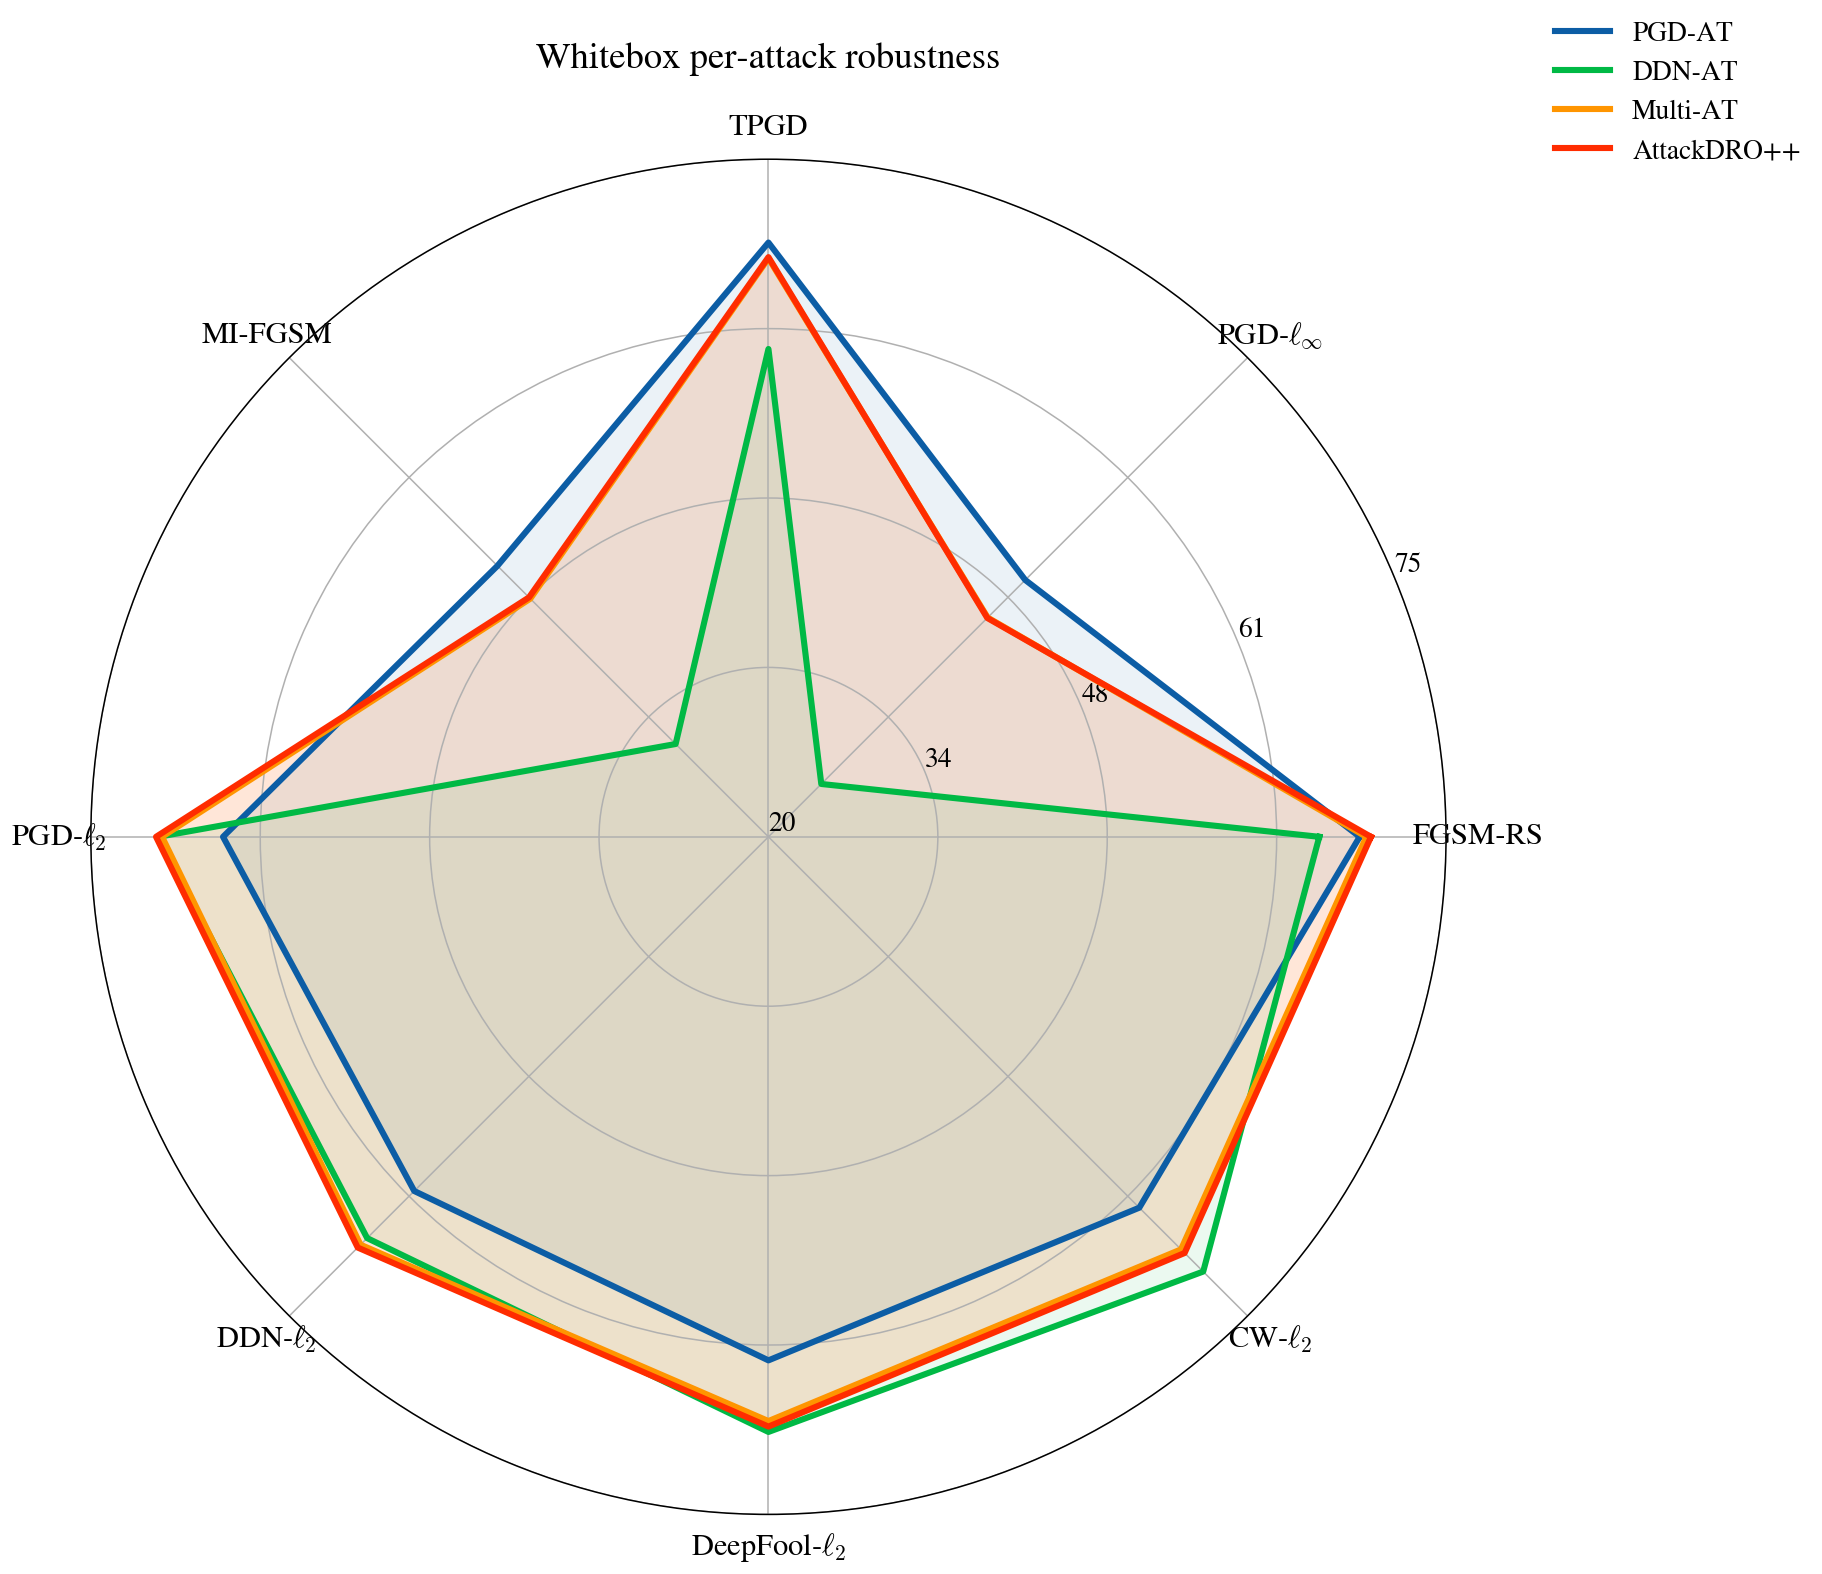
\includegraphics[width=0.78\linewidth]{figures/whitebox/whitebox_radar_per_attack_accuracy_n5.png}
\caption{Whitebox per-attack robustness profile averaged over five seeds. The radar plot compares PGD-AT, DDN-AT, Multi-AT, and AttackDRO++ (Ours) across the eight non-AutoAttack evaluation attacks. The shape of each curve highlights the specialization of the single-attack baselines and the more balanced profile of the multi-attack methods.}
\label{fig:ch6_whitebox_radar_per_attack_accuracy}
\end{figure}

\paragraph{Absolute per-class heatmaps with a shared scale.}
Before analyzing deltas, we first report the raw per-(class $\times$ attack) robust accuracy of each method. All four heatmaps use the same global color scale from 0\% to 100\%. This shared scale is important because it makes the maps visually comparable across methods: a darker cell always represents the same absolute robust accuracy, regardless of which method is being shown. 

\begin{figure}[H]
\centering
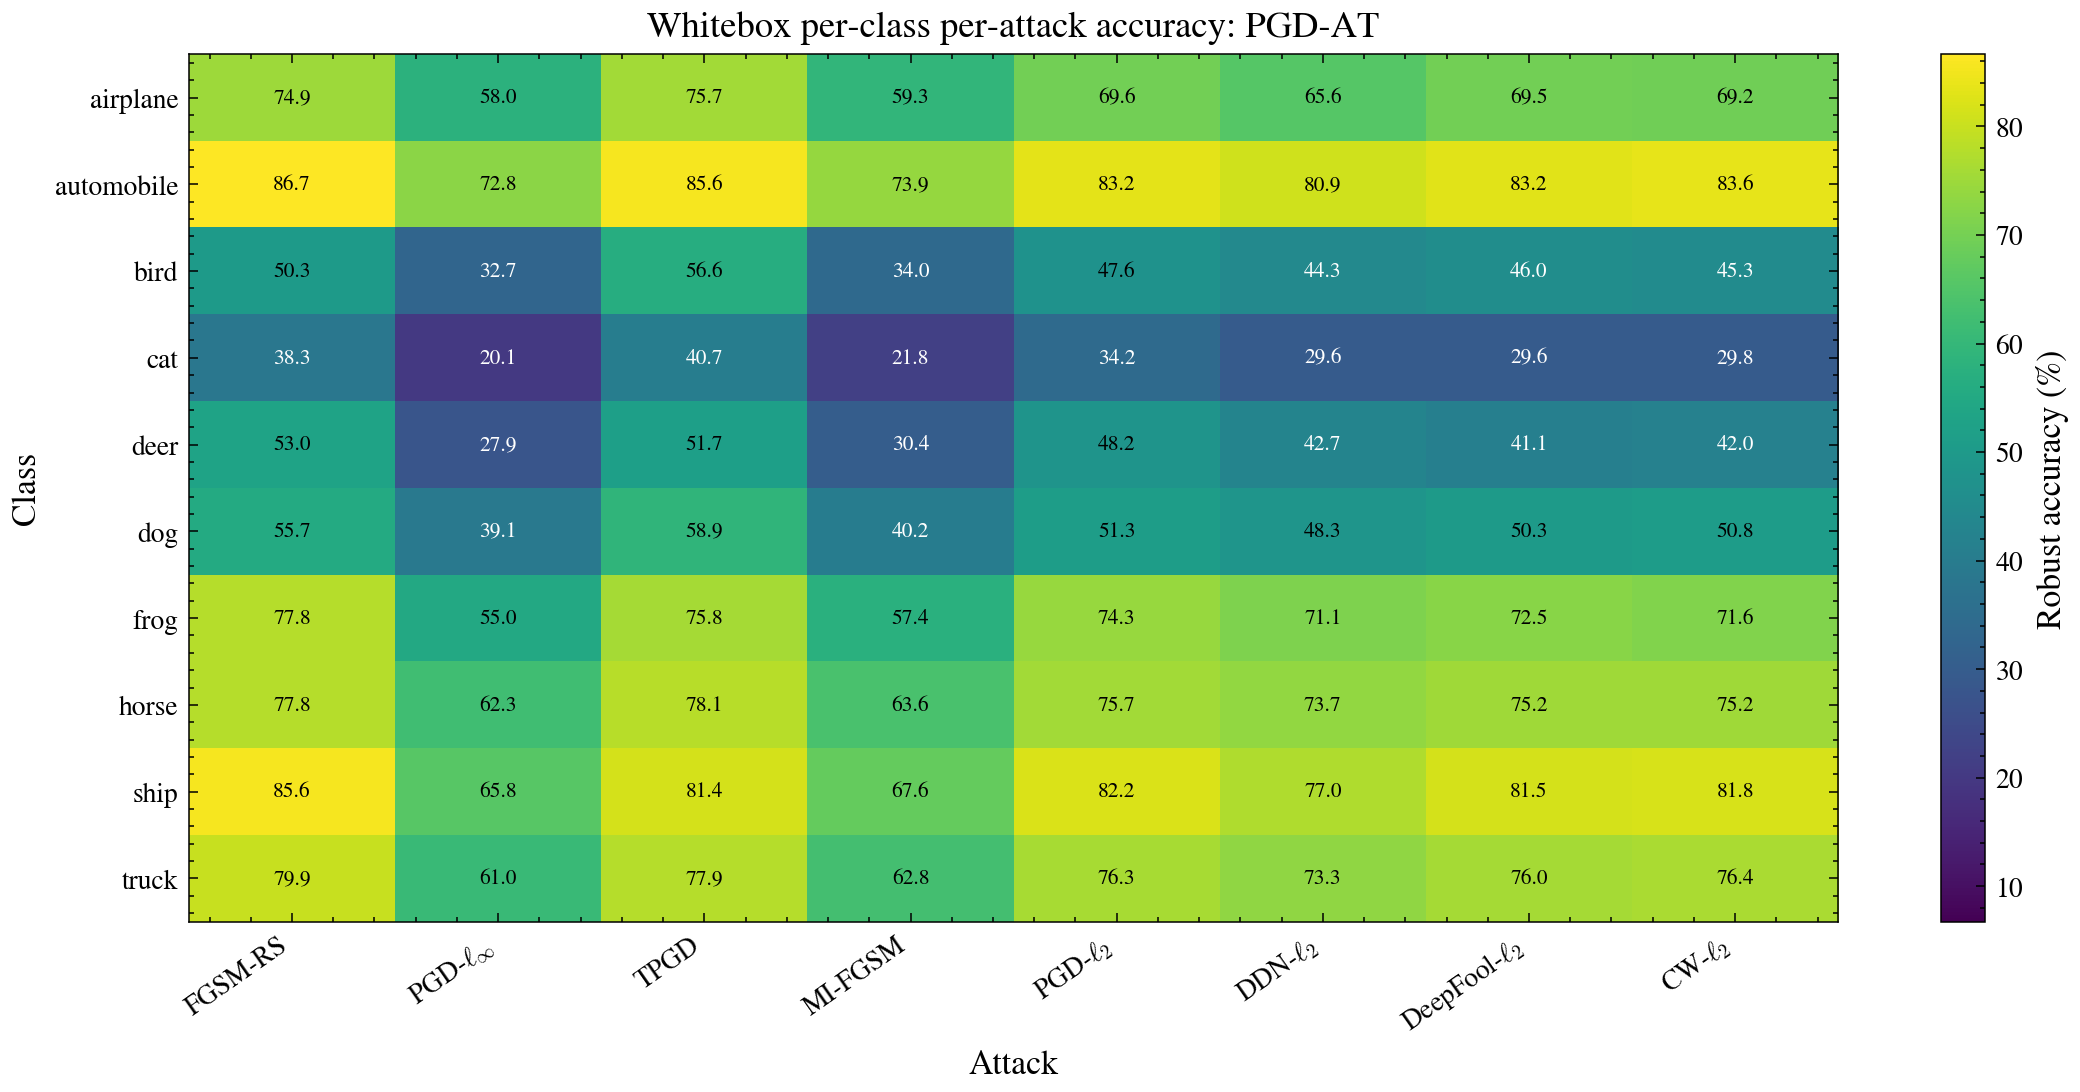
\includegraphics[width=\linewidth]{figures/whitebox/whitebox_per_class_attack_PGDAT_n5.png}
\caption{Absolute whitebox per-(class \(\times\) attack) robust accuracy
for PGD-AT. Cells report robust accuracy (\%).}
\label{fig:ch6_whitebox_abs_pgdat}
\end{figure}

\begin{figure}[H]
\centering
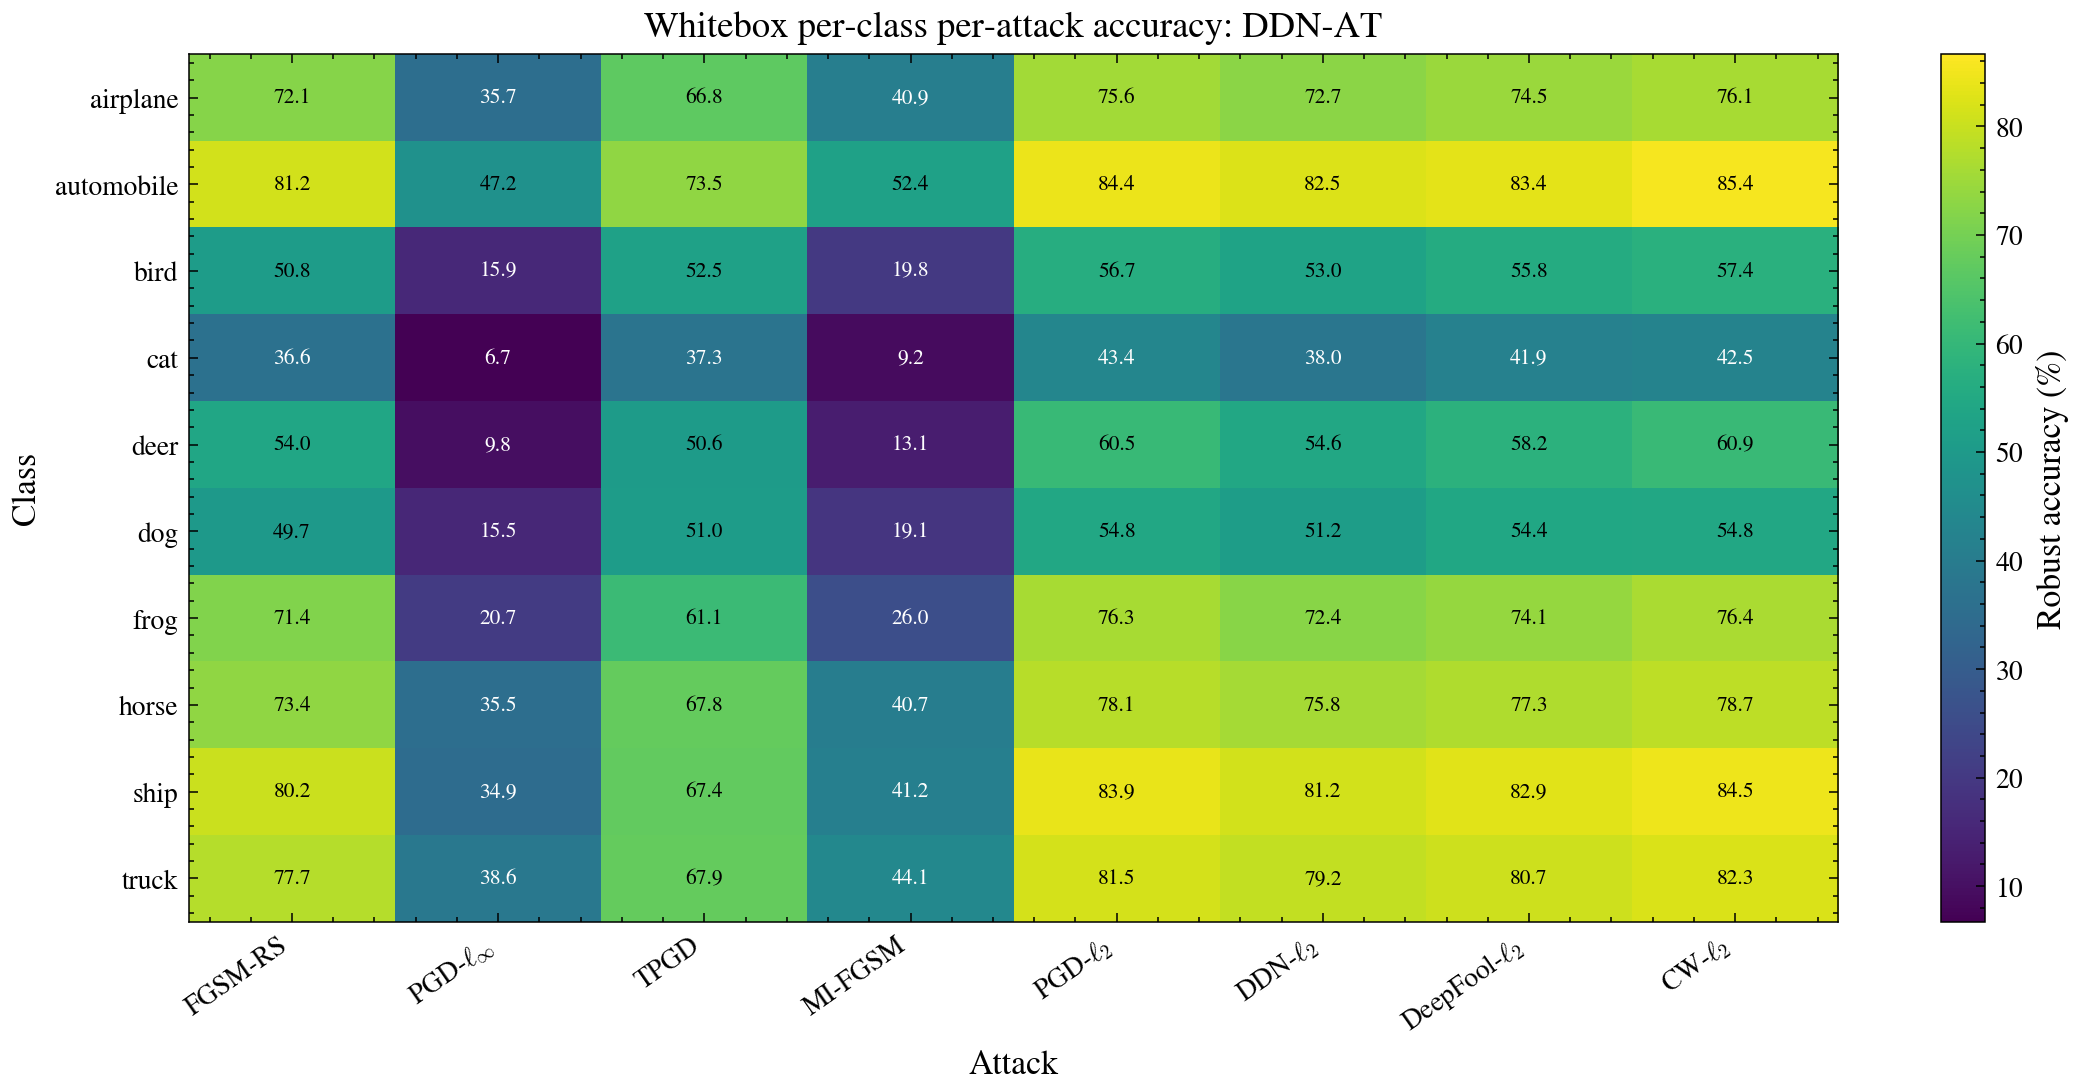
\includegraphics[width=\linewidth]{figures/whitebox/whitebox_per_class_attack_DDNAT_n5.png}
\caption{Absolute whitebox per-(class \(\times\) attack) robust accuracy
for DDN-AT. Cells report robust accuracy (\%).}
\label{fig:ch6_whitebox_abs_ddnat}
\end{figure}

\begin{figure}[H]
\centering
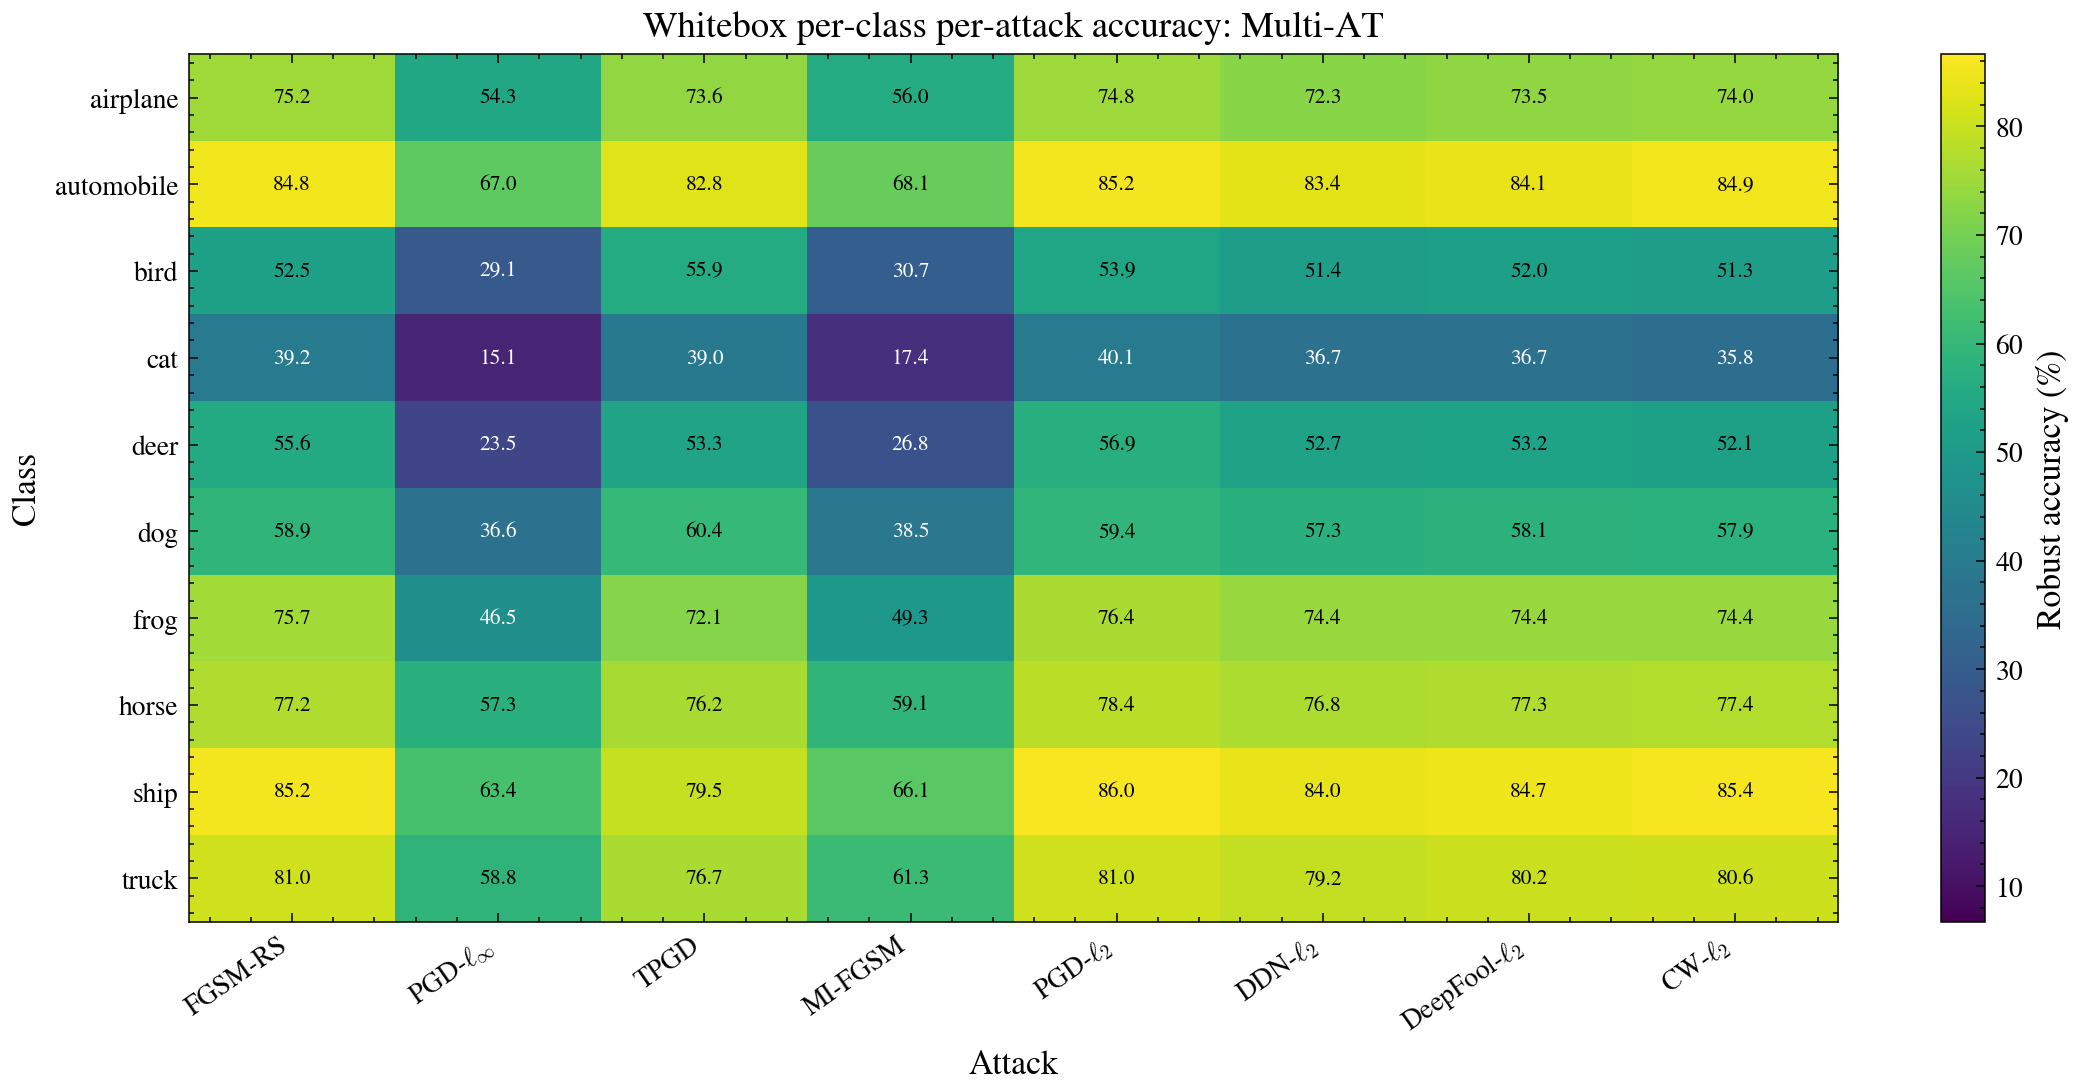
\includegraphics[width=\linewidth]{figures/whitebox/whitebox_per_class_attack_MultiAT_n5.png}
\caption{Absolute whitebox per-(class \(\times\) attack) robust accuracy
for Multi-AT. Cells report robust accuracy (\%).}
\label{fig:ch6_whitebox_abs_multiat}
\end{figure}

\begin{figure}[H]
\centering
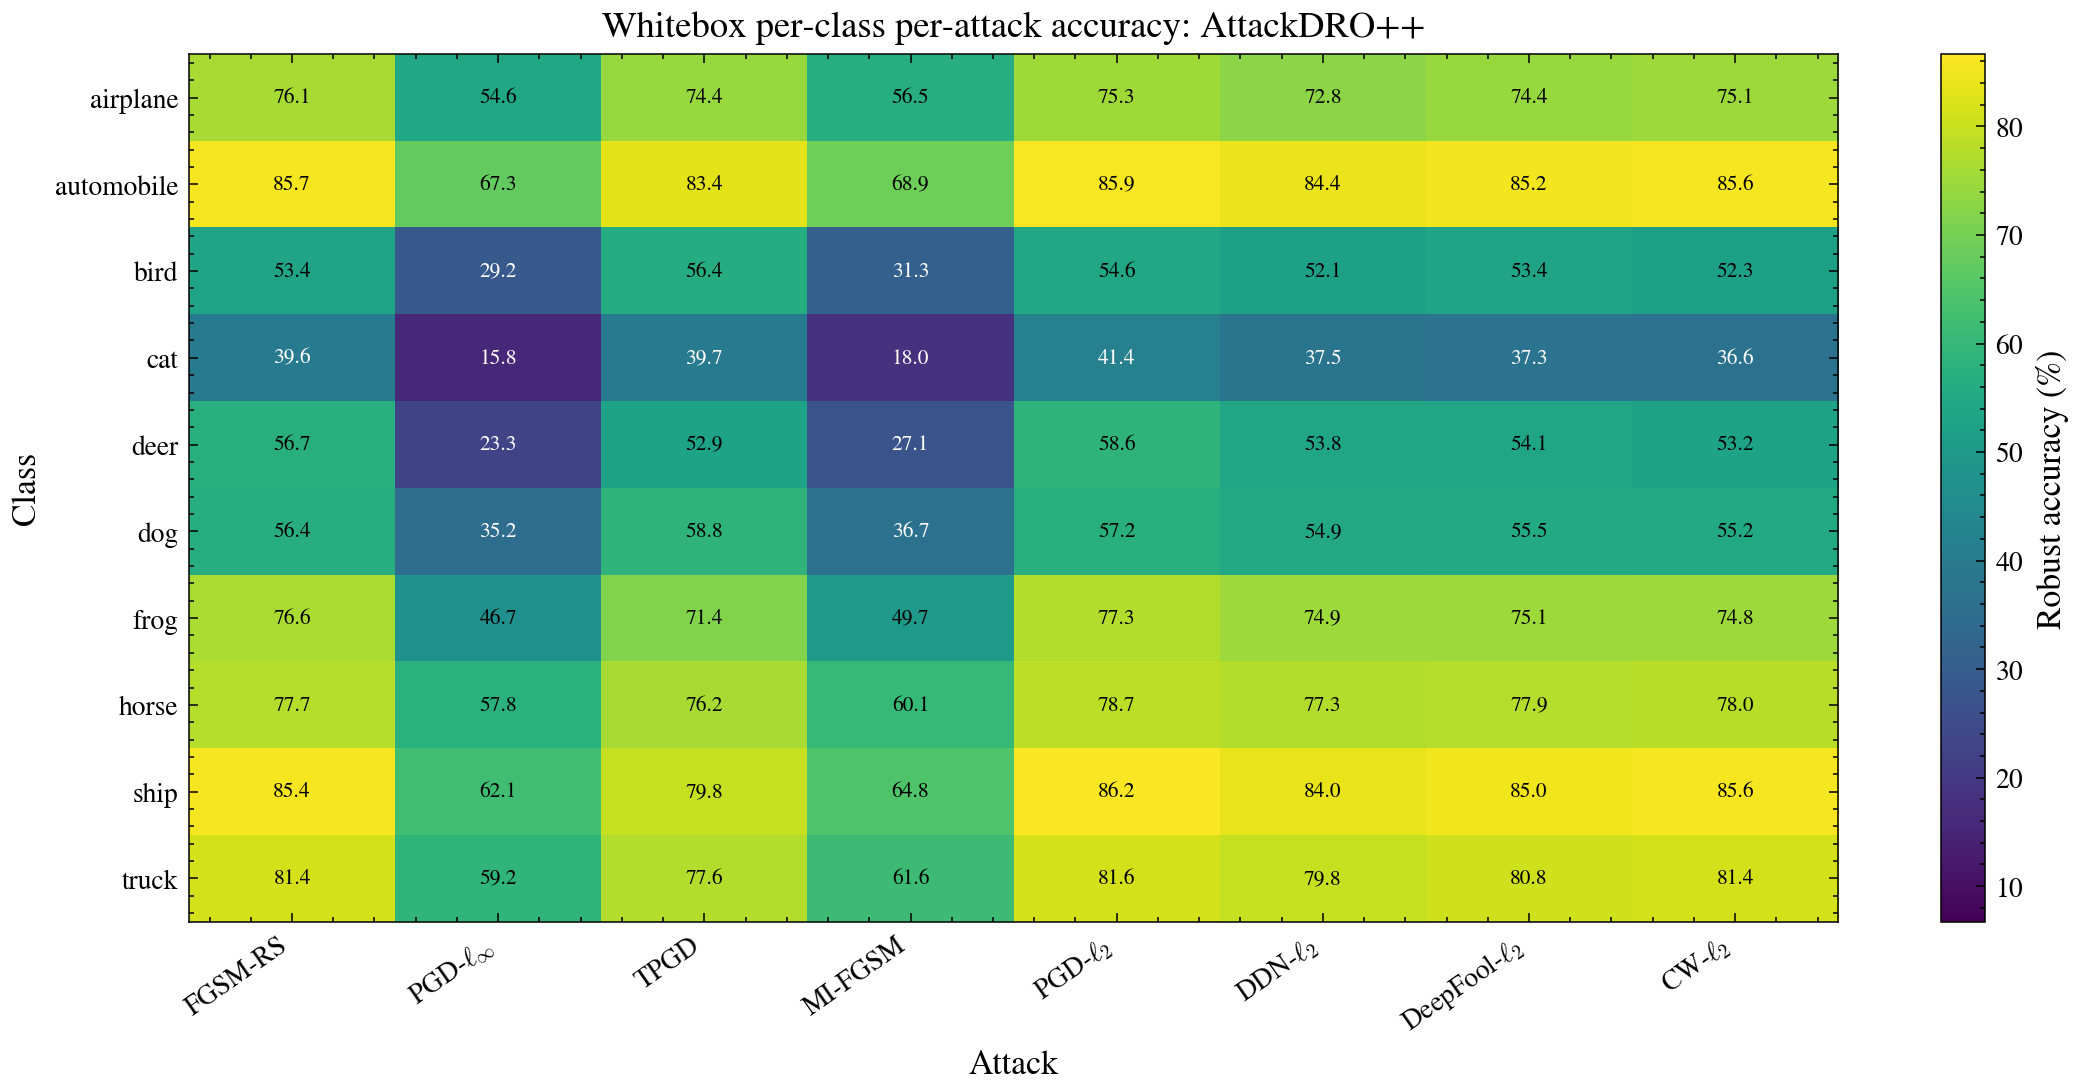
\includegraphics[width=\linewidth]{figures/whitebox/whitebox_per_class_attack_AttackDROpp_n5.png}
\caption{Absolute whitebox per-(class \(\times\) attack) robust accuracy
for AttackDRO++ (Ours). Cells report robust accuracy (\%).}
\label{fig:ch6_whitebox_abs_attackdropp}
\end{figure}
PGD-AT is stronger on several $\ell_\infty$ cells, while DDN-AT is more biased toward bounded $\ell_2$ attacks and visibly weaker on PGD-$\ell_\infty$ and MI-FGSM. Compared with the specialists, Multi-AT and AttackDRO++ show a more balanced cross-attack profile. AttackDRO++ largely preserves the Multi-AT structure while slightly lifting many cells, especially outside the hardest $\ell_\infty$ animal-class tail.

\subsection{Class-Level Gains and Persistent Difficulties}
\label{subsec:ch6_class_level_gains}

% TODO[Kiệt]:
% Goal:
% - Explain the main class-wise patterns without enumerating every class.
% Flow:
% - Identify broad high/low cells, then compare AttackDRO++ against Multi-AT and single-attack specialists.
% Include:
% - Reference `tab:ch6_whitebox_per_cell_summary` and the delta heatmaps.
% Avoid:
% - Unsupported causal claims about why individual CIFAR-10 classes are hard.
% Target length: 3-5 paragraphs.

Across all methods, the per-class robustness pattern is highly non-uniform. Classes such as \textit{automobile}, \textit{ship}, and \textit{truck} tend to remain easier under most attacks, while \textit{cat}, \textit{deer}, \textit{bird}, and \textit{dog} form the recurring hard tail. This pattern is consistent with the visual similarity and intra-class variation of CIFAR-10: animal classes often share local textures and backgrounds, so small adversarial perturbations can more easily move samples across nearby decision regions.

The hardest whitebox cells are concentrated in the $\ell_\infty$ iterative attacks. For AttackDRO++, the lowest cells are PGD-$\ell_\infty$ on \textit{cat} and \textit{deer}, followed by MI-FGSM on the same classes. This indicates that, even though AttackDRO++ improves the average multi-attack profile, the most difficult failure modes are still driven by strong $\ell_\infty$ optimization on semantically similar animal classes. In contrast, bounded $\ell_2$ attacks such as PGD-$\ell_2$, DDN-$\ell_2$, DeepFool-$\ell_2$, and CW-$\ell_2$ are generally less damaging for the proposed model than the strongest $\ell_\infty$ cells.

\paragraph{Attack-Class Delta Against Multi-AT Baseline}
Compared with Multi-AT, AttackDRO++ produces a broad but modest shift rather than a large change concentrated in a few cells. The mean per-cell gain is only $+0.281$ percentage points, but 67 out of 80 attack--class cells are positive.


\begin{figure}[H]
\centering
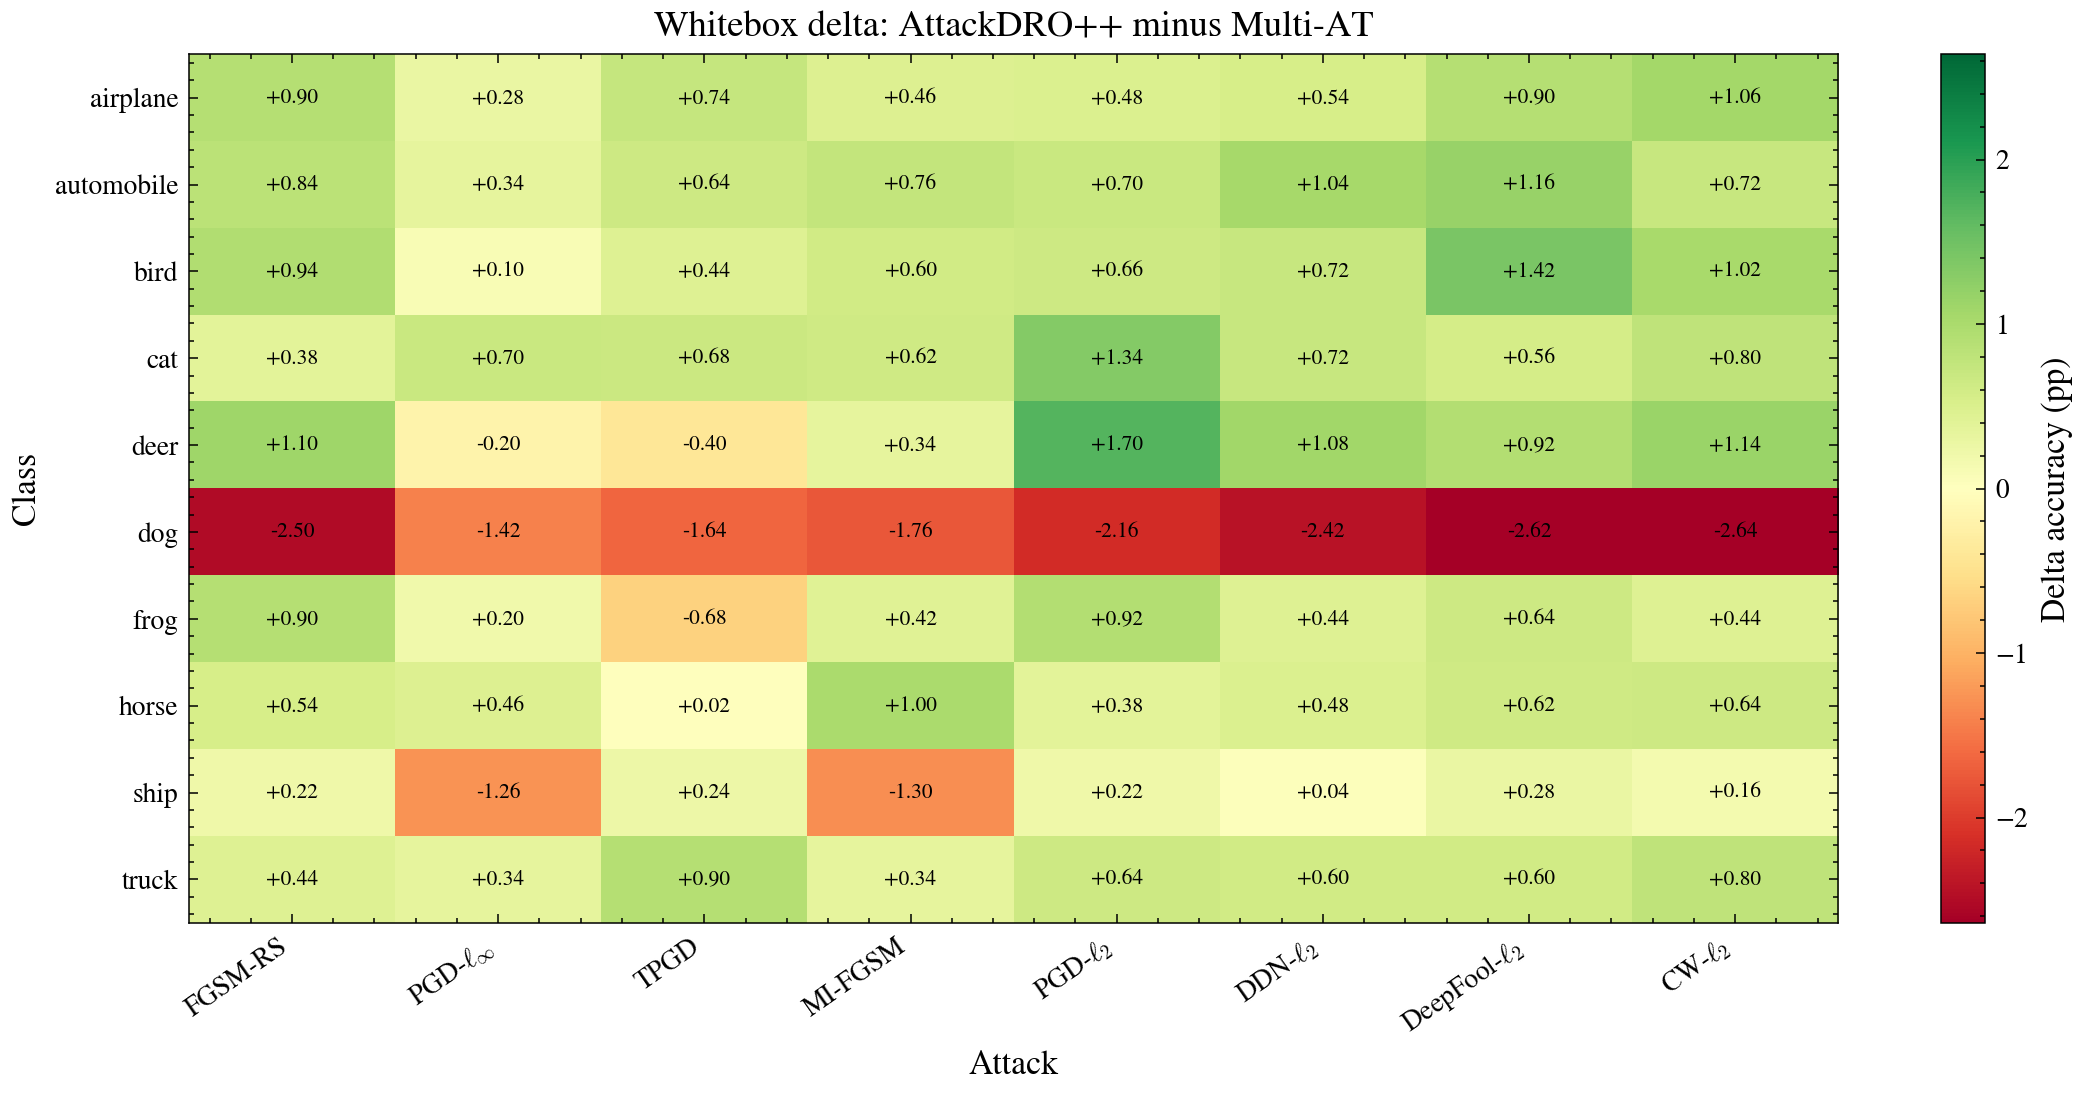
\includegraphics[width=\linewidth]{figures/whitebox/whitebox_delta_per_class_attack_AttackDROpp_vs_MultiAT_n5.png}
\caption{Whitebox per-(class $\times$ attack) delta of AttackDRO++ relative to Multi-AT. Each cell reports AttackDRO++ minus Multi-AT in percentage points, averaged over five seeds.}
\label{fig:ch6_whitebox_delta_vs_multiat}
\end{figure}

\paragraph{Attack-Class Delta Against Single-AT Baselines}

Table~\ref{tab:ch6_whitebox_per_cell_summary} summarizes the per-cell delta between AttackDRO++ and each baseline. The comparison against Multi-AT is the most important one because both methods train on the same source attacks and differ mainly in the group structure used for optimization. AttackDRO++ improves 67/80 cells over Multi-AT, with a mean gain of $+0.281$ percentage points and a bottom-10 lift of $+0.282$ percentage points. The gains are small, but they are widespread, which supports the interpretation that cluster-based DRO acts as a stabilizing refinement over uniform multi-attack training.

\begin{table}[H]
\centering
\caption{Per-(class $\times$ attack) whitebox comparison of AttackDRO++ against each baseline. $\Delta$ is computed as AttackDRO++ minus the baseline. Positive cells count the number of attack--class cells where $\Delta>0$ out of 80 total cells.}
\label{tab:ch6_whitebox_per_cell_summary}
\footnotesize
\setlength{\tabcolsep}{4.5pt}
\renewcommand{\arraystretch}{1.18}
\begin{tabular}{lccccc}
\toprule
Baseline
& Positive cells
& Mean
& Significant cells
& Bottom-10
& Main pattern \\
& $(\Delta>0)$
& $\Delta$ (pp)
& AttackDRO++ / Baseline
& lift (pp)
& \\
\midrule
Multi-AT
& 67/80
& $+0.281$
& 0 / 2
& $+0.282$
& Balanced refinement \\
PGD-AT
& 47/80
& $+1.782$
& 40 / 19
& $+0.726$
& Gains mainly on $\ell_2$ cells \\
DDN-AT
& 62/80
& $+5.781$
& 44 / 5
& $+15.710$
& Gains mainly on $\ell_\infty$ cells \\
\bottomrule
\end{tabular}

\end{table}

\begin{figure}[H]
\centering
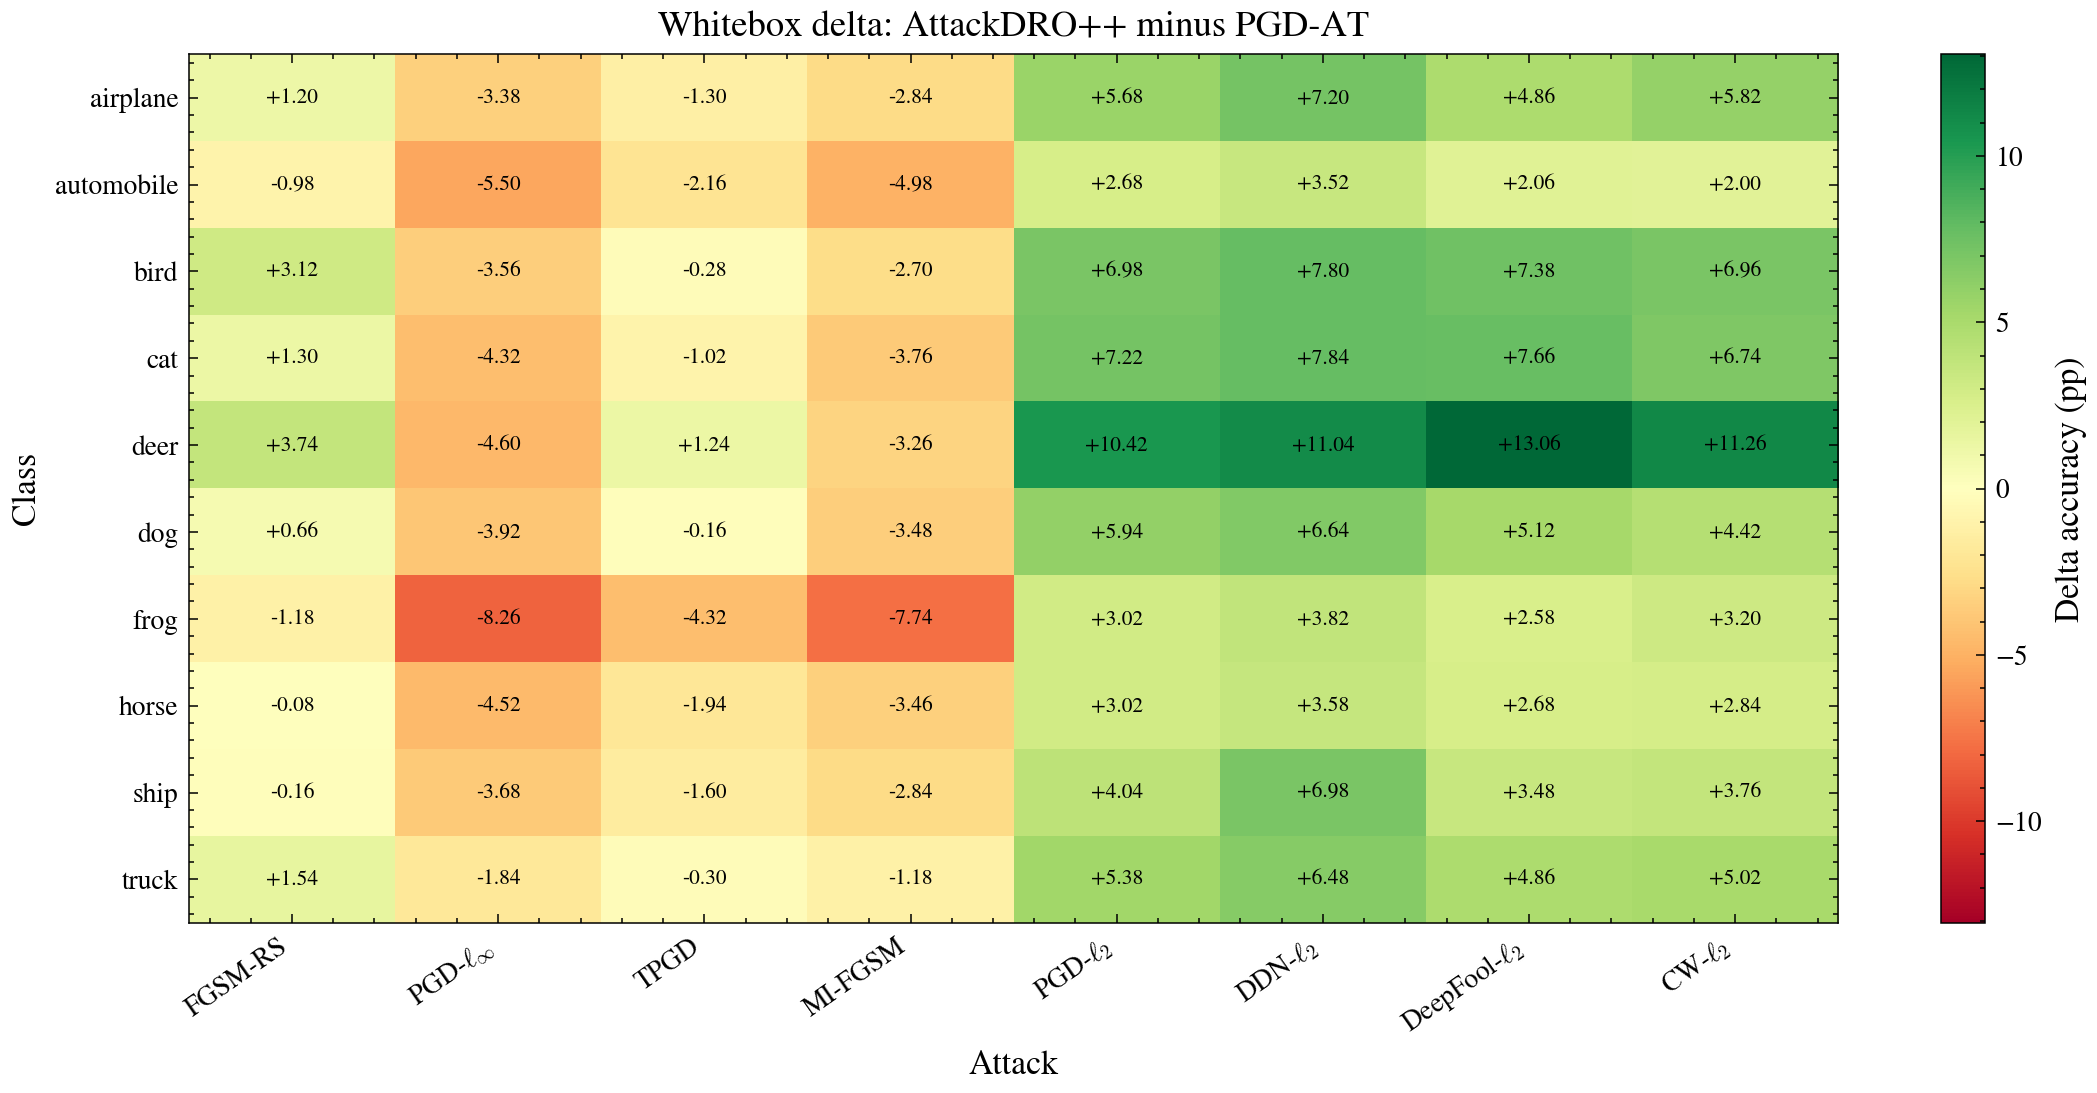
\includegraphics[width=\linewidth]{figures/whitebox/whitebox_delta_per_class_attack_AttackDROpp_vs_PGDAT_n5.png}
\caption{Whitebox per-(class $\times$ attack) delta of AttackDRO++ (Ours) relative to PGD-AT. Positive cells indicate where AttackDRO++ (Ours) improves over the PGD-$\ell_\infty$ specialist. Gains are concentrated mainly on bounded $\ell_2$ attacks, while PGD-AT remains stronger on several $\ell_\infty$ iterative cells.}
\label{fig:ch6_whitebox_delta_vs_pgdat}
\end{figure}

\begin{figure}[H]
\centering
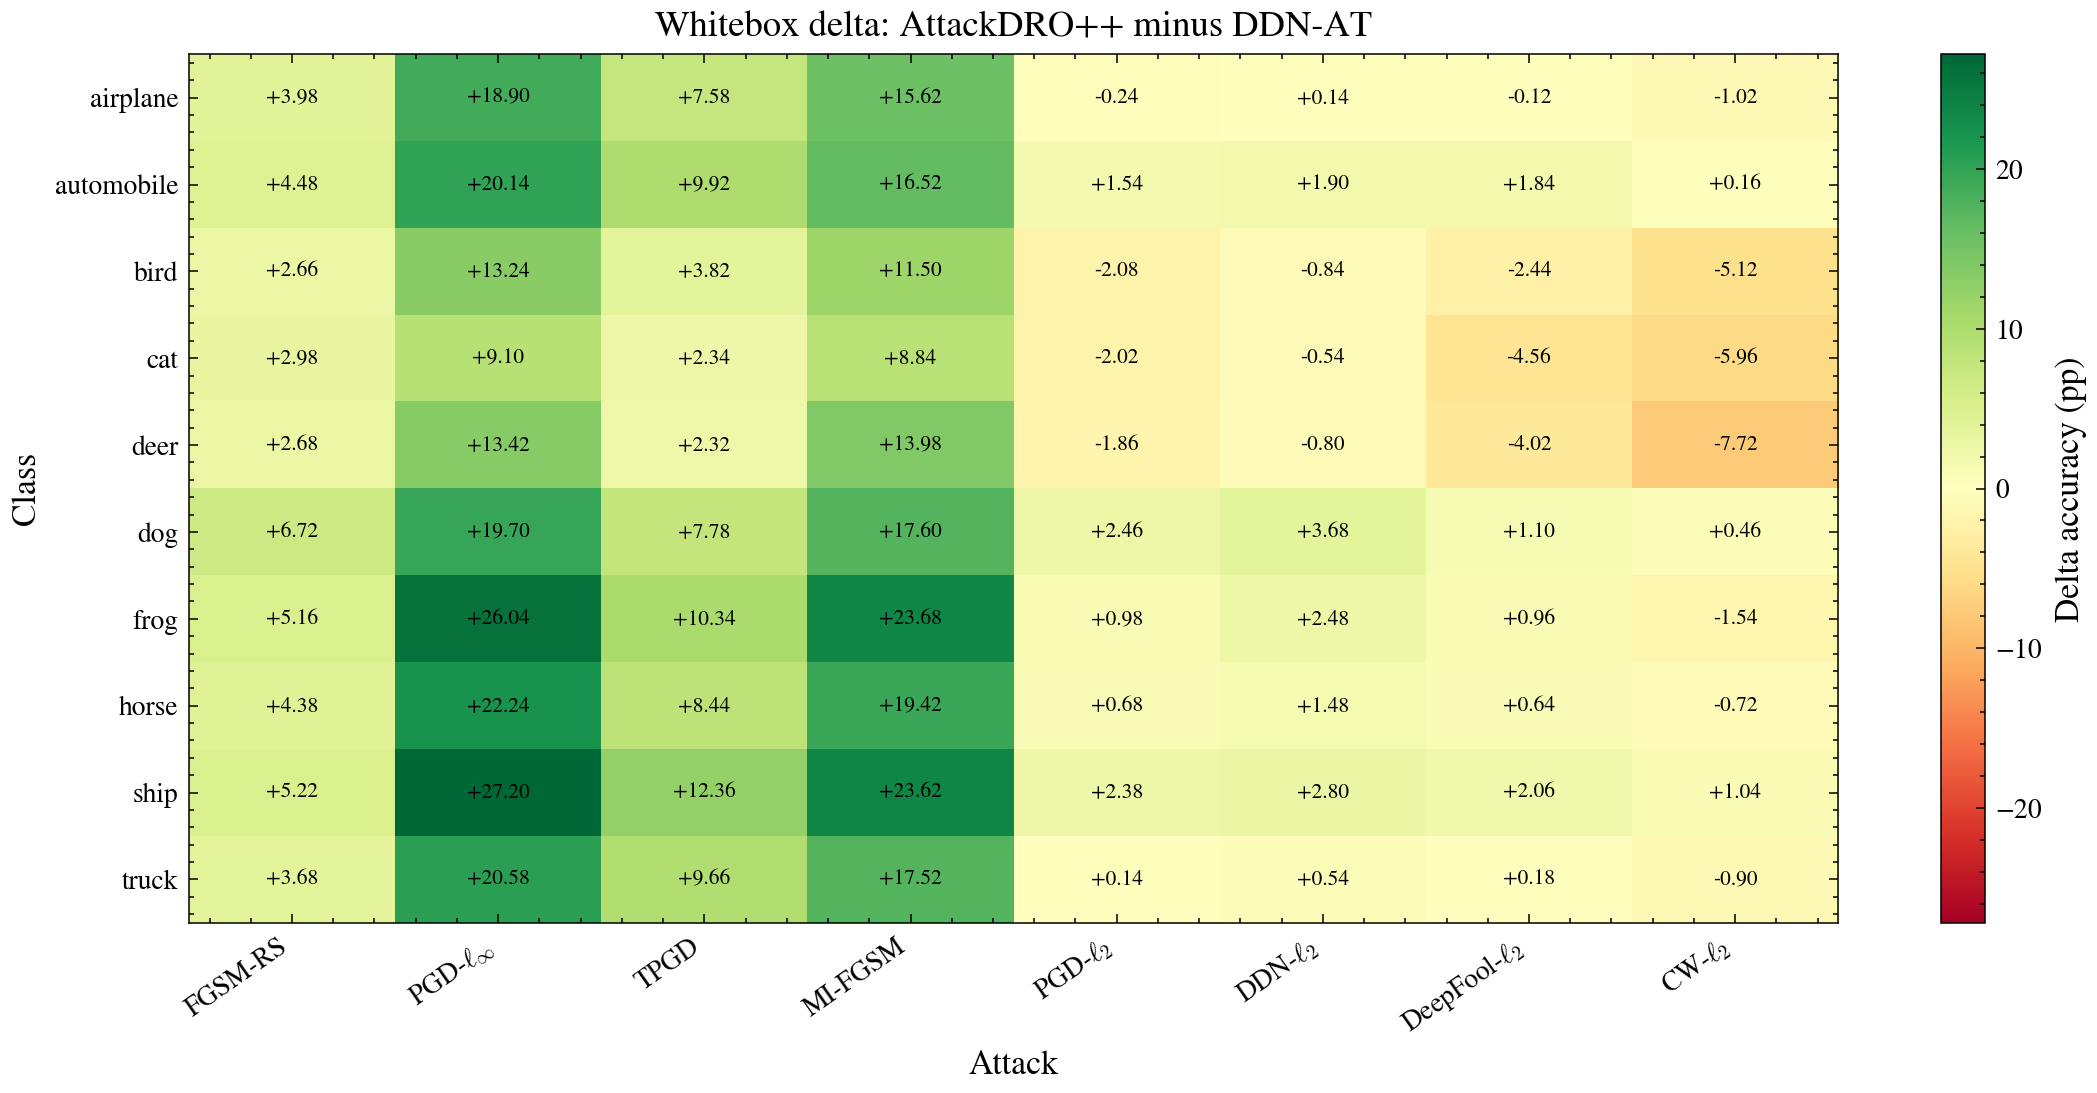
\includegraphics[width=\linewidth]{figures/whitebox/whitebox_delta_per_class_attack_AttackDROpp_vs_DDNAT_n5.png}
\caption{Whitebox per-(class $\times$ attack) delta of AttackDRO++ (Ours) relative to DDN-AT. The large positive cells under PGD-$\ell_\infty$ and MI-FGSM show that AttackDRO++ (Ours) substantially corrects the $\ell_\infty$ weakness of the DDN-$\ell_2$ specialist, while several negative cells remain on DDN-AT's preferred $\ell_2$ family.}
\label{fig:ch6_whitebox_delta_vs_ddnat}
\end{figure}

The comparison against PGD-AT shows the expected specialist trade-off. AttackDRO++ is positive in 47/80 cells and has a mean gain of $+1.782$ percentage points, but the gains and losses are not uniformly distributed. The largest improvements occur on bounded $\ell_2$ attacks, especially DeepFool-$\ell_2$, CW-$\ell_2$, DDN-$\ell_2$, and PGD-$\ell_2$ on hard animal classes such as \textit{deer}, \textit{cat}, and \textit{bird}. For example, the largest gains over PGD-AT appear on DeepFool-$\ell_2$ for \textit{deer} ($+13.06$ pp), CW-$\ell_2$ for \textit{deer} ($+11.26$ pp), and DDN-$\ell_2$ for \textit{deer} ($+11.04$ pp). Conversely, PGD-AT remains stronger on several $\ell_\infty$ cells, particularly PGD-$\ell_\infty$ and MI-FGSM for \textit{frog}, \textit{automobile}, \textit{horse}, and \textit{cat}. This confirms that PGD-AT is not weak in absolute terms; rather, it is specialized toward the $\ell_\infty$ geometry used during training.

The comparison against DDN-AT is even more asymmetric. AttackDRO++ improves 62/80 cells and gains $+5.781$ percentage points on average, with a large $+15.710$ percentage-point improvement on the bottom-10 cells. The largest improvements occur under $\ell_\infty$ attacks: PGD-$\ell_\infty$ on \textit{ship} ($+27.20$ pp), PGD-$\ell_\infty$ on \textit{frog} ($+26.04$ pp), MI-FGSM on \textit{frog} ($+23.68$ pp), and MI-FGSM on \textit{ship} ($+23.62$ pp). These large deltas show that DDN-AT develops a strong $\ell_2$ bias and leaves many $\ell_\infty$ attack--class cells under-protected. At the same time, DDN-AT remains stronger on some $\ell_2$ boundary/optimization cells, especially CW-$\ell_2$ and DeepFool-$\ell_2$ for \textit{deer}, \textit{cat}, and \textit{bird}. Thus, AttackDRO++ improves cross-attack balance but does not completely dominate the strongest single-norm specialist on its preferred family.

\paragraph{Attack-family interpretation.}

% TODO[Kiệt]:
% Goal:
% - Explain whether gains are balanced across attack families.
% Flow:
% - Compare source attacks, held-out `\ell_\infty`, and held-out `\ell_2` patterns.
% Include:
% - Reference the radar delta figure if kept in the main flow.
% Avoid:
% - Using metric shorthand in headings or unexplained captions.
% Target length: 2-4 paragraphs.

The attack-wise deltas make the specialization effect clear. Relative to PGD-AT, AttackDRO++ loses on PGD-$\ell_\infty$ and MI-FGSM on average, but gains strongly on the bounded $\ell_2$ attacks. Relative to DDN-AT, the pattern reverses: AttackDRO++ gains substantially on PGD-$\ell_\infty$, MI-FGSM, TPGD, and FGSM-RS, while being slightly weaker on CW-$\ell_2$ and DeepFool-$\ell_2$. 
The Multi-AT comparison is more balanced: most attack averages are positive, but the magnitudes are below one percentage point.

\begin{figure}[H]
\centering
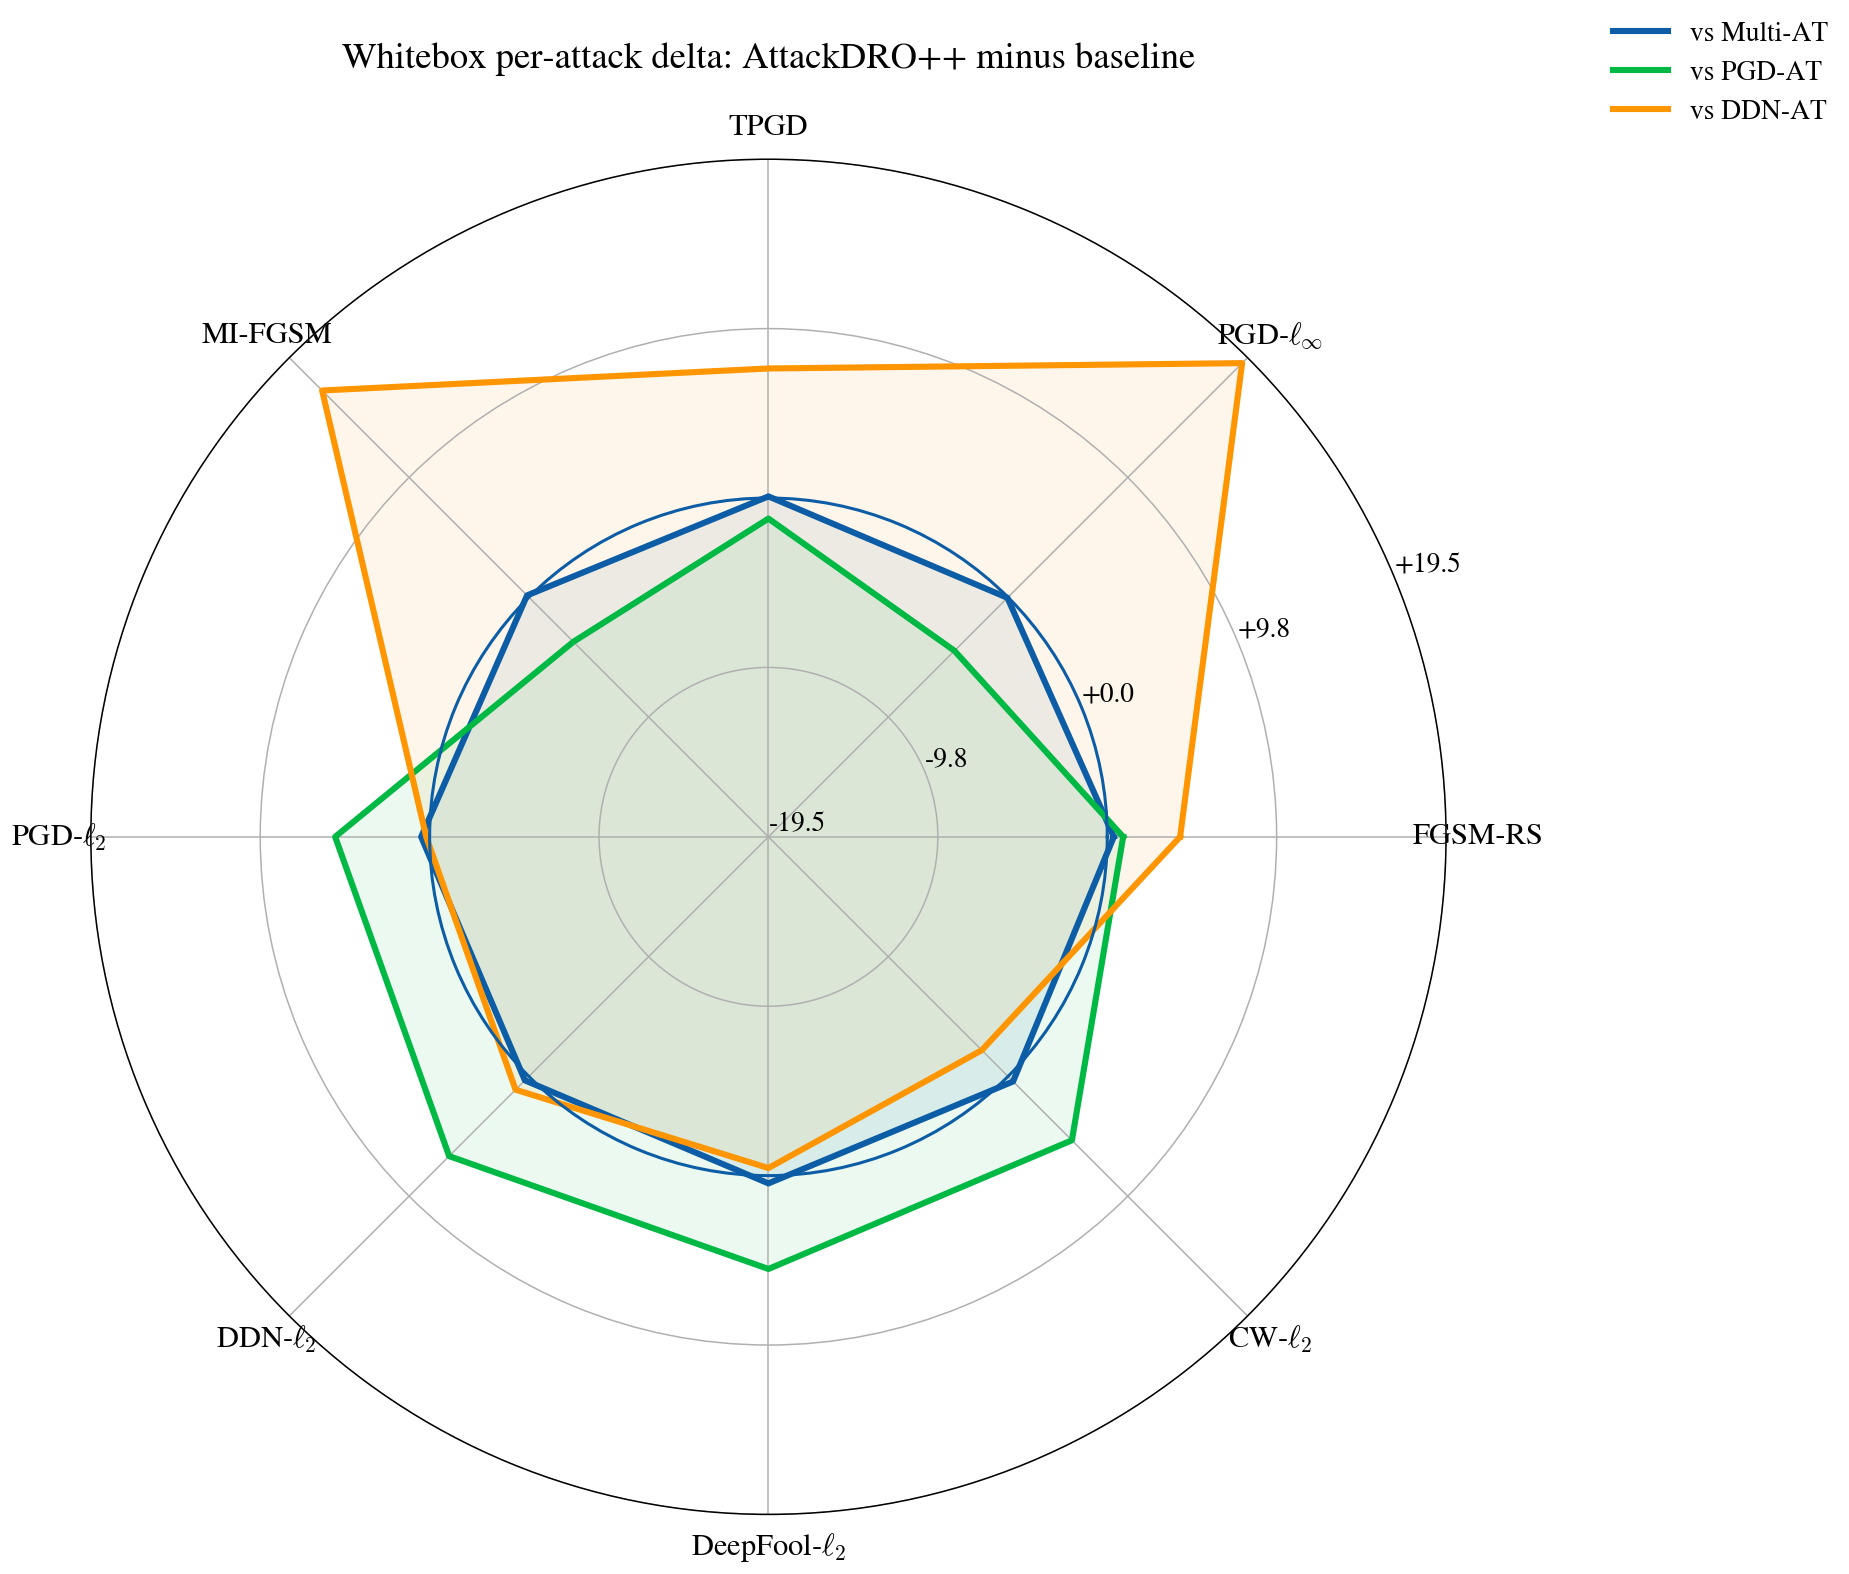
\includegraphics[width=\linewidth]{figures/whitebox/whitebox_radar_attackdropp_delta_vs_baselines_n5.png}
\caption{Attack-wise whitebox delta of AttackDRO++ relative to the three baselines.}
\label{fig:ch6_whitebox_radar_delta_vs_baselines}
\end{figure}
\vspace{-0.5cm}
This result supports the main claim of the chapter. AttackDRO++ should not be interpreted as a replacement for a single specialist when the deployment threat model is known exactly. Instead, it is a cross-attack robustness method: it sacrifices some of the peak strength of a specialist in exchange for a more even robustness profile across attacks and classes. 

\subsection{Tail-Class Robustness: Do the Weakest Cells Improve?}
\label{subsec:ch6_tail_class_robustness}

% TODO[Kiệt]:
% Goal:
% - Explain whether AttackDRO++ improves difficult tail cells, not only average cells.
% Flow:
% - Define Bottom-K locally or point to an earlier definition, then interpret the lift figure.
% Include:
% - Reference `fig:ch6_whitebox_bottomk_lift` if it remains in the main flow.
% Avoid:
% - Leaving `Bottom-K` as undefined shorthand.
% Target length: 2-3 paragraphs.

We next examine the weakest attack--class cells for each baseline, using
\(K \in \{5,10,20\}\). These cells capture localized failure modes that can be
hidden by mean accuracy. For Multi-AT, the weakest cells are mainly strong
\(\ell_\infty\) attacks, especially PGD-$\ell_\infty$ and MI-FGSM, on hard animal
classes such as \textit{cat}, \textit{deer}, and \textit{bird}. AttackDRO++
improves this tail only slightly: the bottom-10 lift is \(+0.282\) pp. Although
small, this shows that the average gain over Multi-AT is not obtained by
sacrificing its weakest cells.

\begin{figure}[H]
\centering
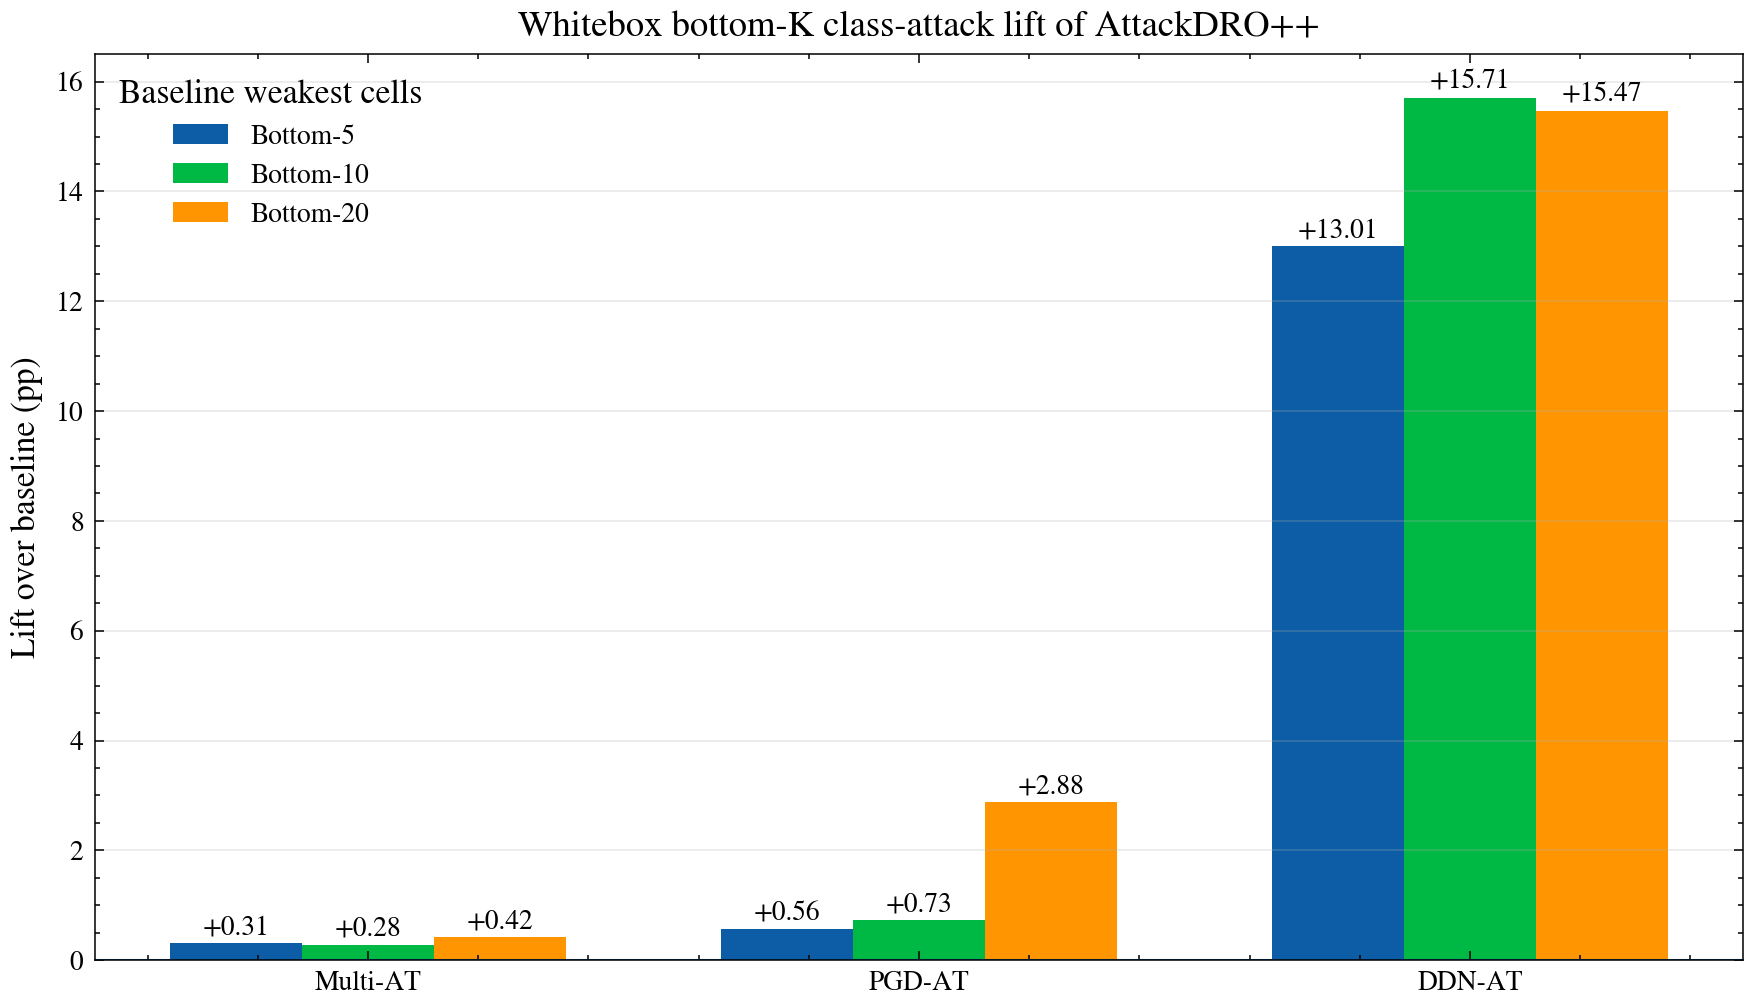
\includegraphics[width=0.64\linewidth]{figures/whitebox/whitebox_bottomk_lift_bar_n5.png}
\caption{Weakest-\(K\) whitebox class--attack lift of AttackDRO++ over each
baseline. For each baseline, the weakest-\(K\) cells are the lowest-accuracy
class--attack cells of that baseline; bars report AttackDRO++ minus the
baseline on those same cells.}
\label{fig:ch6_whitebox_bottomk_lift}
\end{figure}

The tail comparison is most pronounced against DDN-AT. Its weakest cells collapse
under \(\ell_\infty\)-oriented attacks, with the bottom-10 cells averaging only
\(15.602\%\). AttackDRO++ raises these same cells by \(+15.710\) pp, explaining
why it achieves a much more balanced whitebox profile than the \(\ell_2\)
specialist, even though DDN-AT remains competitive on several \(\ell_2\) cells.

Against PGD-AT, the lift is smaller but still positive: \(+0.726\) pp on the
bottom-10 cells. PGD-AT's weakest cells include several bounded \(\ell_2\)
attacks on difficult classes such as \textit{cat} and \textit{deer}; AttackDRO++
reduces many of these failures, indicating that multi-attack training and the
Cluster-DRO component help mitigate the cross-norm weakness of PGD-only training.

Overall, the weakest-cell analysis supports the aggregate conclusion from
Section~\ref{sec:ch6_whitebox}: AttackDRO++ gives a broad but modest refinement
over Multi-AT, substantially corrects the \(\ell_\infty\) tail weakness of
DDN-AT, and reduces the \(\ell_2\) tail weakness of PGD-AT.

The class-wise whitebox analysis shows where the aggregate gains appear and
which hard cells remain. It still evaluates attacks generated directly against
the target checkpoint, so it does not answer whether the same robustness pattern
holds when adversarial examples are crafted on a different model. The next
section therefore moves to the graybox transfer protocol from
Section~\ref{sec:ch5_graybox_protocol}.


% ─────────────────────────────────────────────────────────────────────────────
\newpage
\section{Graybox Robustness Across Surrogate Models}
\label{sec:ch6_graybox}

% TODO[Kiệt]:
% Goal:
% - Explain graybox robustness as transfer behavior, not just another accuracy table.
% Flow:
% - Start with protocol sanity, then transfer matrices, pairwise comparisons, gap analysis, per-cell analysis, and decomposition.
% Include:
% - Cite active figures/tables from docs/04_figure_table_registry.md, especially currently unreferenced graybox tables/figures if kept.
% Avoid:
% - Overclaiming deployment transfer beyond the surrogate/target protocol.
% Target length: 6-9 pages depending on consolidation.
% ─────────────────────────────────────────────────────────────────────────────

The whitebox results in Section~\ref{sec:ch6_whitebox} show that
AttackDRO++ improves average and held-out robustness over Multi-AT on
\(n=20\) paired seeds. We next test whether this gain also holds under
cross-model transfer, using the graybox protocol of
Section~\ref{sec:ch5_graybox_protocol}. In this setting, adversarial examples
are generated on one checkpoint and evaluated on an independently trained
target checkpoint.

\paragraph{Random-seed checkpoint panel and whitebox sanity check.}

% TODO[Kiệt]:
% Goal:
% - Justify the random-seed checkpoint panel and show it is consistent with the main whitebox trends.
% Flow:
% - Explain the fixed random-seed panel, then interpret `tab:ch6_graybox_whitebox_sanity`.
% Include:
% - State clearly that this is a sanity check, not the main 20-seed whitebox result.
% Avoid:
% - Repeating full Chapter 6.1 results.
% Target length: 2-3 paragraphs.

The graybox analysis uses 20 random-seed checkpoints to define the
surrogate--target evaluation panel. These checkpoints come from four method
families evaluated across five random seeds each and are fixed before graybox
transfer is analyzed. The diagonal sanity check below compares this
random-seed checkpoint panel against the full whitebox panel to verify that the
main method ordering is preserved.

The diagonal entries of the graybox table correspond to the case where
the surrogate and target are the same checkpoint. We use these entries as
a whitebox sanity check. They need not match the main whitebox evaluation
exactly, because the graybox cache uses a balanced
125-image-per-class-per-attack split instead of the full test set for
each attack. However, they should preserve the same method ordering and
remain close in absolute value.

\begin{table}[H]
\centering
\caption{Whitebox sanity check from the graybox pipeline. The \(n=5\)
columns use diagonal graybox entries, where surrogate and target are the
same checkpoint. The \(n=20\) columns report the main whitebox results
from Table~\ref{tab:ch6_aggregate_results}.}
\label{tab:ch6_graybox_whitebox_sanity}
\small
\setlength{\tabcolsep}{6pt}
\renewcommand{\arraystretch}{1.08}
\begin{tabular}{lrrrr}
\toprule
Target method
& Mean(8) \(n=5\)
& Worst(8) \(n=5\)
& Mean(8) \(n=20\)
& Worst(8) \(n=20\) \\
\midrule
PGD-AT
& $61.524$ & $\mathbf{50.384}$ & $60.499$ & $\mathbf{49.656}$ \\
DDN-AT
& $56.922$ & $25.568$ & $56.226$ & $25.957$ \\
Multi-AT
& $62.458$ & $45.584$ & $62.045$ & $45.082$ \\
AttackDRO++ (Ours)
& $\mathbf{62.642}$ & $45.088$ & $\mathbf{62.324}$ & $45.079$ \\
\bottomrule
\end{tabular}
\end{table}

The Mean(8) ordering is identical on both panels --- AttackDRO++ $>$
Multi-AT $>$ PGD-AT $>$ DDN-AT --- and absolute values agree to within
$1.0$~pp. More importantly, the paired Mean(8) delta of AttackDRO++ minus
Multi-AT is $+0.184$~pp on the $n=5$ graybox panel and
$+0.279$~pp on the full $n=20$ panel: both are positive and of the same
order of magnitude. The graybox cache is therefore consistent with the
main evaluation protocol and supports the cross-method analyses below.

\subsection{Cross-Method Transfer Structure}
\label{subsec:ch6_graybox_transfer_structure}

% TODO[Kiệt]:
% Goal:
% - Explain how to read the graybox transfer matrices and what off-diagonal transfer means.
% Flow:
% - Define row/column roles, then interpret aggregate and per-attack matrices.
% Include:
% - Reference `fig:ch6_graybox_transfer_matrix`, `fig:ch6_graybox_transfer_linf`, and `fig:ch6_graybox_transfer_l2`.
% Avoid:
% - Treating diagonal whitebox cells as graybox evidence.
% Target length: 3-5 paragraphs.

We aggregate the per-attack per-class transfer table into a method-level
$4 \times 4$ transfer matrix. Rows index the target method being evaluated, and columns index the
surrogate method that generates adversarial examples. Each cell reports
the target robust accuracy averaged over all matching target--surrogate
seed pairs and the eight evaluation attacks. Higher values indicate that
the row target is more robust to adversarial examples crafted on the
column surrogate.

\begin{figure}[H]
\centering
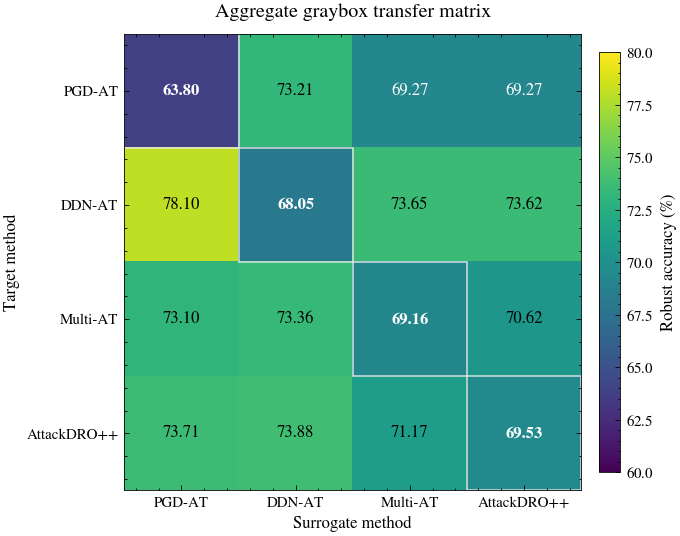
\includegraphics[width=0.78\linewidth]{figures/graybox/graybox_transfer_matrix_4method_aggregate_science_clean.png}
\caption{Method-level graybox transfer matrix on the \(n=5\) panel.
Rows are target methods and columns are surrogate methods. Cell values
are robust accuracy (\%) averaged over seeds and the eight evaluation
attacks.}
\label{fig:ch6_graybox_transfer_matrix}
\end{figure}

Two structural patterns are visible. First, rows ranked by mean
off-diagonal accuracy give DDN-AT ($75.12\%$) $>$ AttackDRO++ ($72.92\%$)
$>$ Uniform Multi-AT ($72.36\%$) $>$ PGD-AT ($70.59\%$). The DDN-AT
row is highest not because DDN-AT is the strongest defense --- its
whitebox Mean(8) is the lowest of the four --- but because $\ell_\infty$
adversarial examples generated by other surrogates transfer poorly to a
DDN-AT target whose decision boundary is shaped by $\ell_2$ training.
Section~\ref{subsec:ch6_paired_graybox_comparisons} quantifies this structural inflation
explicitly through the whitebox--graybox gap. Second, the AttackDRO++
row is consistently above the Uniform Multi-AT row for every surrogate,
with cross-method gaps ranging from $+0.17$~pp (DDN-AT surrogate) to
$+0.61$~pp (PGD-AT surrogate). The whitebox advantage of AttackDRO++
over Uniform Multi-AT therefore persists when adversarial examples are
crafted on independently trained surrogates.

The aggregate transfer matrix hides important attack-family structure.
Figures~\ref{fig:ch6_graybox_transfer_linf} and~\ref{fig:ch6_graybox_transfer_l2}
therefore disaggregate the transfer behavior into the four
\(\ell_\infty\)-oriented attacks and the four \(\ell_2\)-oriented attacks.
This grouping makes the specialist behavior more explicit. 

\begin{figure}[H]
\centering
\begin{minipage}{0.48\linewidth}
  \centering
  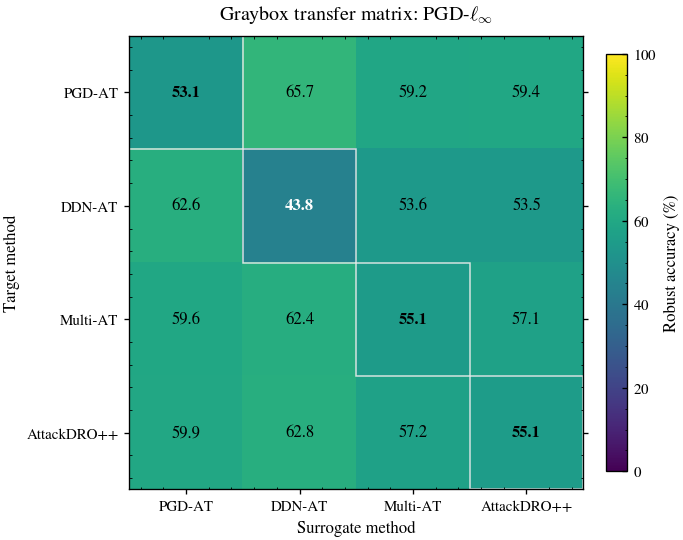
\includegraphics[width=\linewidth]{figures/graybox/transfer_matrix_4method_pgd20_ce_science_clean.png}
  \\ \footnotesize (a) PGD-\(\ell_\infty\)
\end{minipage}\hfill
\begin{minipage}{0.48\linewidth}
  \centering
  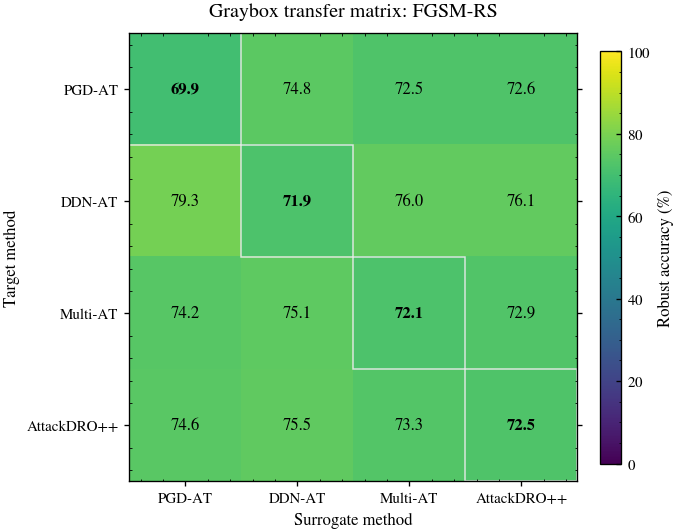
\includegraphics[width=\linewidth]{figures/graybox/transfer_matrix_4method_fgsm_rs_science_clean.png}
  \\ \footnotesize (b) FGSM-RS
\end{minipage}

\vspace{0.6em}

\begin{minipage}{0.48\linewidth}
  \centering
  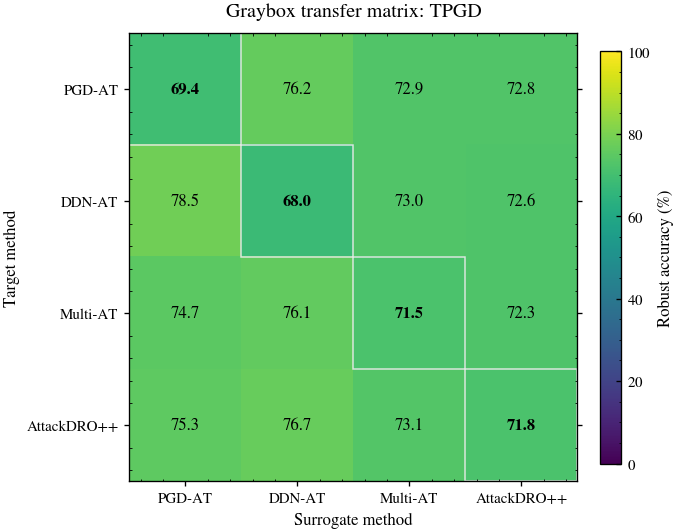
\includegraphics[width=\linewidth]{figures/graybox/transfer_matrix_4method_tpgd_science_clean.png}
  \\ \footnotesize (c) TPGD
\end{minipage}\hfill
\begin{minipage}{0.48\linewidth}
  \centering
  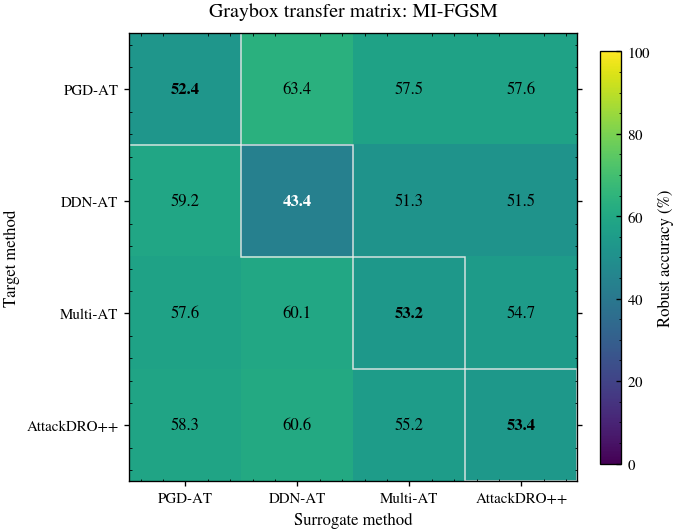
\includegraphics[width=\linewidth]{figures/graybox/transfer_matrix_4method_mifgsm_science_clean.png}
  \\ \footnotesize (d) MI-FGSM
\end{minipage}

\caption{Per-attack graybox transfer matrices for the
\(\ell_\infty\)-oriented attacks. Rows are target methods and columns
are surrogate methods; cells report robust accuracy (\%).}
\label{fig:ch6_graybox_transfer_linf}
\end{figure}

On the
\(\ell_\infty\) attacks, this advantage disappears: PGD-AT and
AttackDRO++ are more competitive, and AttackDRO++ remains closer to the
balanced Multi-AT profile. Thus, the per-attack matrices show that
DDN-AT's strong graybox row average should be interpreted as
family-specific transfer specialization rather than uniform robustness.

\begin{figure}[H]
\centering
\begin{minipage}{0.48\linewidth}
  \centering
  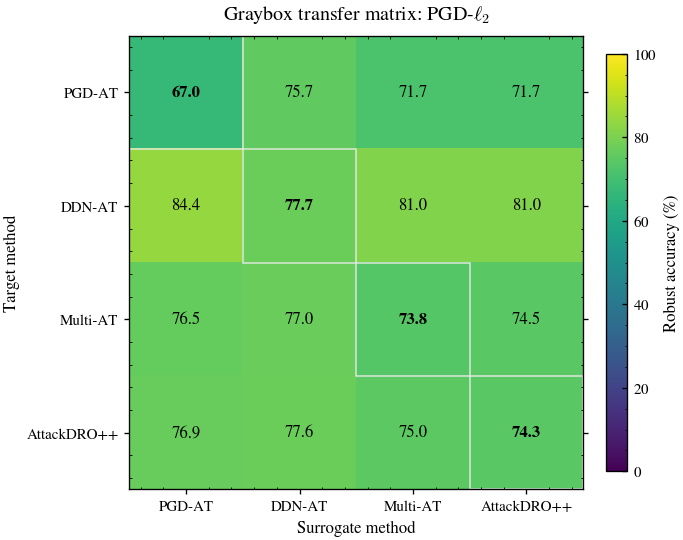
\includegraphics[width=\linewidth]{figures/graybox/transfer_matrix_4method_pgd_l2_science_clean.png}
  \\ \footnotesize (a) PGD-\(\ell_2\)
\end{minipage}\hfill
\begin{minipage}{0.48\linewidth}
  \centering
  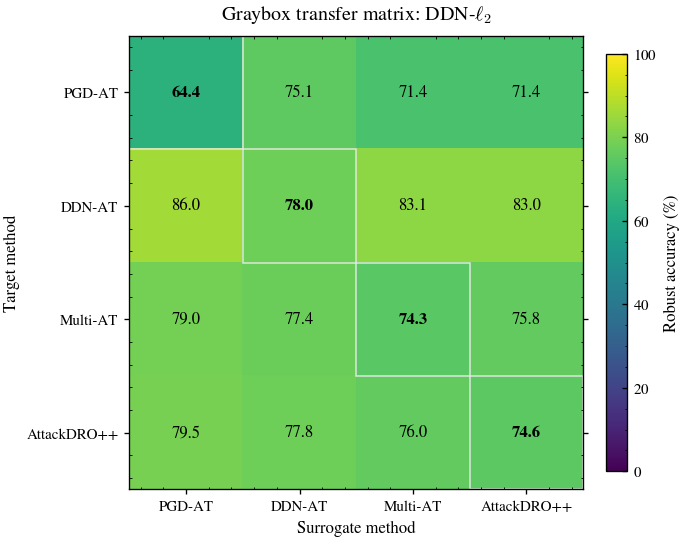
\includegraphics[width=\linewidth]{figures/graybox/transfer_matrix_4method_ddn_l2_science_clean.png}
  \\ \footnotesize (b) DDN-\(\ell_2\)
\end{minipage}

\vspace{0.6em}

\begin{minipage}{0.48\linewidth}
  \centering
  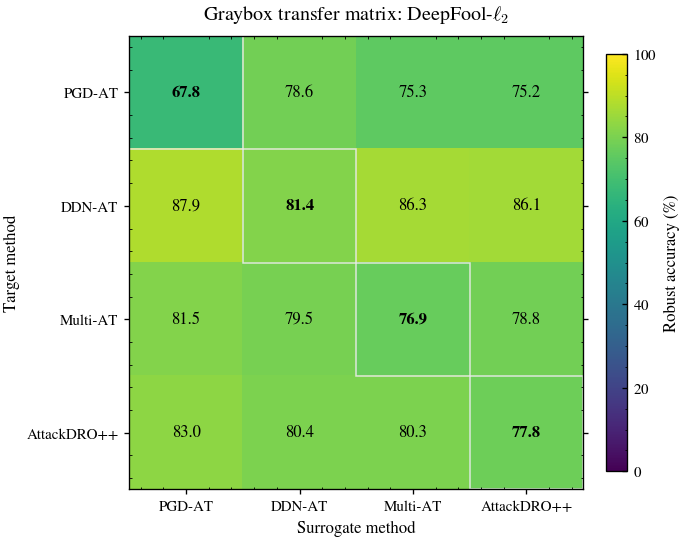
\includegraphics[width=\linewidth]{figures/graybox/transfer_matrix_4method_deepfool_l2_science_clean.png}
  \\ \footnotesize (c) DeepFool-\(\ell_2\)
\end{minipage}\hfill
\begin{minipage}{0.48\linewidth}
  \centering
  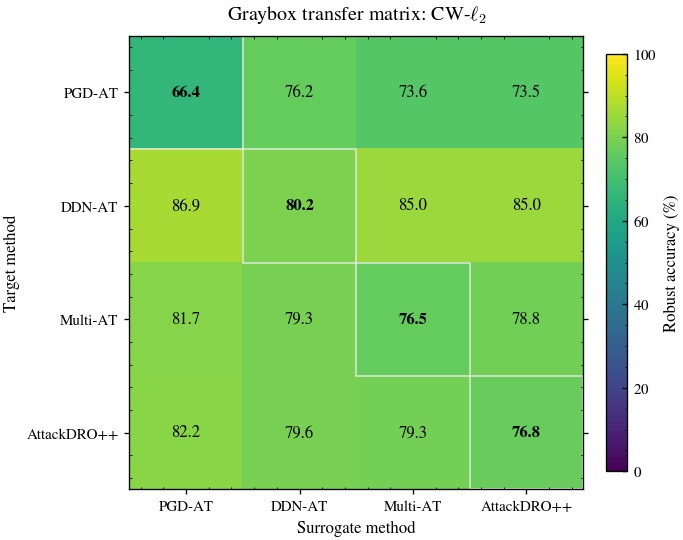
\includegraphics[width=\linewidth]{figures/graybox/transfer_matrix_4method_cw_l2_science_clean.png}
  \\ \footnotesize (d) CW-\(\ell_2\)
\end{minipage}

\caption{Per-attack graybox transfer matrices for the
\(\ell_2\)-oriented attacks. Rows are target methods and columns are
surrogate methods; cells report robust accuracy (\%).}
\label{fig:ch6_graybox_transfer_l2}
\end{figure}
On the \(\ell_2\) attacks, the DDN-AT target row is consistently strong,
especially when attacks are transferred from PGD-AT, Multi-AT, or
AttackDRO++ surrogates. This indicates that DDN-AT's high aggregate
graybox score is driven mainly by \(\ell_2\)-family transfer behavior,
rather than by uniformly strong robustness across both attack geometries.
AttackDRO++ remains closer to the balanced Multi-AT profile, while still
improving over Multi-AT on most \(\ell_2\)-oriented transfer cells.


\subsection{Paired Graybox Comparisons: Does the Whitebox Advantage Carry Over?}
\label{subsec:ch6_paired_graybox_comparisons}

% TODO[Kiệt]:
% Goal:
% - Compare AttackDRO++ against the strongest uniform multi-attack baseline under graybox transfer.
% Flow:
% - Interpret paired graybox tests, then identify where the advantage is robust or limited.
% Include:
% - Reference `tab:ch6_paired_graybox_two_panel` and `tab:ch6_graybox_attack_family`.
% Avoid:
% - Ignoring corrected p-values or effect size when discussing differences.
% Target length: 3-5 paragraphs.

The main graybox comparison is between AttackDRO++ and Multi-AT.
Both methods train on the same source attacks
$\{\text{PGD-}\ell_\infty,\ \text{DDN-}\ell_2\}$ and use the same backbone
and schedule; they differ only in the use of latent clustering, gradient
fingerprints, and the anchored Cluster-DRO objective.

We use the symmetric paired test that has already been described in
Section~\ref{sec:ch5_graybox_protocol}: for every triple
$(\text{target seed},\ \text{surrogate seed},\ \text{attack})$, we pair
the configuration ``AttackDRO++ as target, Multi-AT as surrogate'' against
its mirror ``Multi-AT as target, AttackDRO++ as surrogate'' and compute
the per-triple difference. As the results, $n = 5 \times 5 \times 8 = 200$
paired pairs make the comparison invariant to which method is chosen as
the surrogate.
\begin{table}[H]
\centering
\caption{Paired graybox comparisons. Each row uses $n=200$ paired
target--surrogate--attack triples. Positive $\Delta$ favors the reference
method named in the panel heading.}
\label{tab:ch6_paired_graybox_two_panel}
\begin{tabular}{lcccccc}
\toprule
Compared method
& \multicolumn{2}{c}{Accuracy}
& $\Delta$
& $d_z$
& $t$
& $p$ \\
\cmidrule(lr){2-3}
& Reference
& Baseline
& (pp)
& 
& 
&  \\
\midrule

\multicolumn{7}{l}{\textit{AttackDRO++ (Ours) vs. baselines}} \\
\midrule
Multi-AT
& 71.17
& 70.62
& +0.549
& 0.42
& 5.96
& \textbf{$1.1{\times}10^{-8}$} \\

PGD-AT
& 73.71
& 69.27
& \textbf{+4.435}
& 1.33
& 18.78
& \textbf{$6.1{\times}10^{-46}$} \\

DDN-AT
& 73.88
& 73.62
& +0.258
& 0.04
& 0.60
& 0.549 \\

\midrule
\multicolumn{7}{l}{\textit{Multi-AT vs. single-attack baselines}} \\
\midrule
PGD-AT
& 73.10
& 69.27
& \textbf{+3.829}
& 1.19
& 16.89
& \textbf{$2.7{\times}10^{-40}$} \\

DDN-AT
& 73.36
& 73.65
& $-0.292$
& $-0.05$
& $-0.67$
& 0.504 \\

\bottomrule
\end{tabular}
\end{table}

The AttackDRO++ vs. Multi-AT contrast is the headline result of
this section: under symmetric cross-method graybox transfer,
AttackDRO++ improves onMulti-AT by $+0.549$~pp at
$p \approx 1.1 \times 10^{-8}$, with a small-to-medium paired effect size
of $d_z \approx 0.42$. This effect is roughly twice the corresponding
whitebox delta of $+0.279$~pp on the same seed panel and is significant
at far stricter levels. The Cluster-DRO improvement therefore
\emph{strengthens} rather than disappears under graybox transfer,
indicating that the gain originates from a broader cross-attack
robustness profile rather than from a defense narrowly tuned to
AttackDRO++'s own gradients.

The single-attack contrasts confirm the expected specialist--versus--balanced
pattern. AttackDRO++ improves on PGD-AT by $+4.44$~pp at
$p < 10^{-45}$ ($d_z = 1.33$, a large effect), tracking the whitebox
trend that PGD-AT loses heavily on the $\ell_2$ family it does not train
against. The AttackDRO++ vs.\ DDN-AT contrast is statistically
indistinguishable from zero ($+0.26$~pp, $p = 0.55$); this reflects the
DDN-AT graybox inflation discussed above, not actual parity. We dissect
this asymmetry in Section~\ref{subsec:ch6_paired_graybox_comparisons}.

\paragraph{Per-attack transfer behavior.}

% TODO[Kiệt]:
% Goal:
% - Identify which attacks drive graybox transfer differences.
% Flow:
% - Discuss per-attack table, then connect attack-family behavior to whitebox findings.
% Include:
% - Reference `tab:ch6_graybox_per_attack` if retained in the main flow.
% Avoid:
% - Duplicating the transfer-matrix discussion.
% Target length: 2-4 paragraphs.

To check whether the $+0.549$~pp Mean(8) gain over Multi-AT is
broad or concentrated, we report paired graybox deltas attack by attack
on the same $n=200$ pair set. Each attack contributes $25$ paired
triples (one per surrogate--target seed combination).

\begin{table}[H]
\centering
\caption{Per-attack symmetric graybox comparison between AttackDRO++
and Multi-AT. Each attack uses \(n=25\) paired seed combinations.
Bold deltas are significant at \(p<0.05\).}
\label{tab:ch6_graybox_per_attack}
\small
\setlength{\tabcolsep}{4pt}
\renewcommand{\arraystretch}{1.10}
\begin{tabular}{llrrrr}
\toprule
Attack          & Family              & A mean (\%) & B mean (\%) & $\Delta$ (pp) & $p$ \\
\midrule
FGSM-RS         & held-out $\ell_\infty$ & $73.32$ & $72.86$ & $\mathbf{+0.454}$ & $0.0114$ \\
PGD-$\ell_\infty$ & seen $\ell_\infty$    & $57.17$ & $57.07$ & $+0.102$ & $0.307$  \\
TPGD            & held-out $\ell_\infty$ & $73.09$ & $72.30$ & $\mathbf{+0.790}$ & $0.0240$ \\
MI-FGSM         & held-out $\ell_\infty$ & $55.20$ & $54.75$ & $\mathbf{+0.458}$ & $0.0022$ \\
\midrule
PGD-$\ell_2$    & held-out $\ell_2$      & $74.97$ & $74.53$ & $\mathbf{+0.432}$ & $0.0373$ \\
DDN-$\ell_2$    & seen $\ell_2$          & $76.04$ & $75.79$ & $+0.256$ & $0.341$  \\
DeepFool-$\ell_2$ & held-out $\ell_2$    & $80.29$ & $78.82$ & $\mathbf{+1.469}$ & $0.0002$ \\
CW-$\ell_2$     & held-out $\ell_2$      & $79.26$ & $78.83$ & $+0.429$ & $0.249$  \\
\bottomrule
\end{tabular}
\end{table}

AttackDRO++ produces a positive paired delta on all eight attacks. Five
of these deltas are individually significant at $p < 0.05$, and the gain
is largest on DeepFool-$\ell_2$ ($+1.47$~pp, $p = 1.6\times 10^{-4}$),
the most local-gradient $\ell_2$ attack and the held-out attack on which
the whitebox gain over Multi-AT was also largest. The two seen
attacks (PGD-$\ell_\infty$ and DDN-$\ell_2$) contribute small,
non-significant gains, consistent with the fact that both methods
already train against these attacks. The graybox Mean(8) gain is
therefore distributed across attack families rather than concentrated on
one family.

We aggregate the per-attack deltas into the four attack groups defined
in Section~\ref{sec:ch5_evaluation_metrics} to compare the cross-method graybox
profile across all four methods.

\begin{table}[H]
\centering
\caption{Cross-method graybox accuracy by attack family. Values are
off-diagonal target accuracy (\%) averaged over the \(n=5\) panel.
Bold values mark the best method in each column.}
\label{tab:ch6_graybox_attack_family}
\small
\setlength{\tabcolsep}{6pt}
\renewcommand{\arraystretch}{1.08}
\begin{tabular}{lrrrrr}
\toprule
Target method     & Seen $\ell_\infty$ & Seen $\ell_2$ & Heldout $\ell_\infty$ & Heldout $\ell_2$ & Mean(8) \\
\midrule
PGD-AT & $\mathbf{61.48}$ & $72.61$ & $68.93$           & $74.60$           & $70.59$ \\
DDN-AT      & $56.58$          & $\mathbf{84.03}$ & $68.60$ & $\mathbf{84.85}$  & $\mathbf{75.12}$ \\
Multi-AT  & $59.71$          & $77.40$          & $68.64$ & $78.62$           & $72.36$ \\
AttackDRO++ (Ours) & $59.96$          & $77.78$          & $\mathbf{69.18}$ & $79.35$ & $72.92$ \\
\bottomrule
\end{tabular}
\end{table}

The family decomposition makes three points concrete. The held-out
$\ell_\infty$ column has AttackDRO++ at the top ($69.18\%$) by a small
but consistent margin over the other three methods. The held-out
$\ell_2$ column is dominated by DDN-AT ($84.85\%$), with AttackDRO++
($79.35\%$) ranked second and improving on Multi-AT by
$+0.73$~pp. The seen $\ell_2$ column shows the same pattern. The seen
$\ell_\infty$ column favors PGD-AT, again by structure: surrogates
generate strong PGD-$\ell_\infty$ adversarial examples, and only PGD-AT
is robust to them. AttackDRO++ is the only method that is at or above
Multi-AT on every attack family, while DDN-AT and PGD-AT each
remain narrow specialists under transfer.

\paragraph{Whitebox--graybox gap and specialist inflation.}

% TODO[Kiệt]:
% Goal:
% - Explain the gap between direct whitebox robustness and transferred robustness.
% Flow:
% - Define the gap sign, interpret `tab:ch6_graybox_gap`, then use heatmaps for method-specific patterns.
% Include:
% - Reference gap heatmaps from `fig:ch6_graybox_gap_ddnat` to `fig:ch6_graybox_gap_attackdropp`.
% - Add caption polish later for sign/unit/averaging conditions.
% Avoid:
% - Treating large whitebox scores alone as evidence of transferable robustness.
% Target length: 3-5 paragraphs.

The DDN-AT target row in Figure~\ref{fig:ch6_graybox_transfer_matrix} and
the DDN-AT row in Table~\ref{tab:ch6_graybox_attack_family} are the highest
under graybox transfer,
even though DDN-AT has the lowest whitebox Mean(8) on both the $n=5$ and
the full $n=20$ panels. We resolve this apparent contradiction by
quantifying the gap between whitebox and cross-method graybox accuracy
for each method. A large positive gap indicates that a defense looks
much stronger under graybox transfer than under direct whitebox attack,
which is a signature of a structural transfer mismatch rather than a
broader robustness profile.

\begin{table}[H]
\centering
\caption{Whitebox--graybox gap by target method on the \(n=5\) panel.
The gap is cross-method graybox Mean(8) minus diagonal whitebox Mean(8).}
\label{tab:ch6_graybox_gap}
\small
\setlength{\tabcolsep}{8pt}
\renewcommand{\arraystretch}{1.08}
\begin{tabular}{lrrr}
\toprule
Target method     & Whitebox Mean(8) & Graybox Mean(8) & Gap (pp) \\
\midrule
PGD-AT & $61.52$ & $70.59$ & $\phantom{0}+9.06$  \\
DDN-AT      & $56.92$ & $75.12$ & $\mathbf{+18.20}$   \\
Multi-AT  & $62.46$ & $72.36$ & $\phantom{0}+9.90$  \\
AttackDRO++ (Ours) & $\mathbf{62.64}$ & $72.92$ & $+10.27$   \\
\bottomrule
\end{tabular}
\end{table}

PGD-AT, Multi-AT, and AttackDRO++ all show a comparable
whitebox--graybox gap of approximately $9$--$10$~pp, indicating that
adversarial examples crafted on alternate surrogates are weaker than
those crafted directly on the target by a roughly constant amount.
DDN-AT, by contrast, gains $+18.20$~pp under graybox transfer, almost
twice the gap of any other method. Its row-leading graybox accuracy is therefore not evidence of a stronger defense; it is an artifact of
how poorly $\ell_\infty$ adversarial examples generated by PGD-AT, Multi-AT, and AttackDRO++ surrogates transfer to a
purely-$\ell_2$-trained target. AttackDRO++ retains the highest whitebox
Mean(8) of the four methods while exhibiting a graybox gap that is only
$+0.37$~pp larger than that of Multi-AT --- consistent with a
balanced cross-attack defense rather than a transfer-favored
specialist.

The per-(class \(\times\) attack) whitebox--graybox gap heatmaps in
Figures~\ref{fig:ch6_graybox_gap_ddnat}--\ref{fig:ch6_graybox_gap_attackdropp}
make the specialist-inflation effect concrete. Cell values are computed
as graybox accuracy minus whitebox accuracy, so positive values indicate
that transferred attacks are weaker than direct whitebox attacks on the
same target.

\begin{figure}[H]
\centering
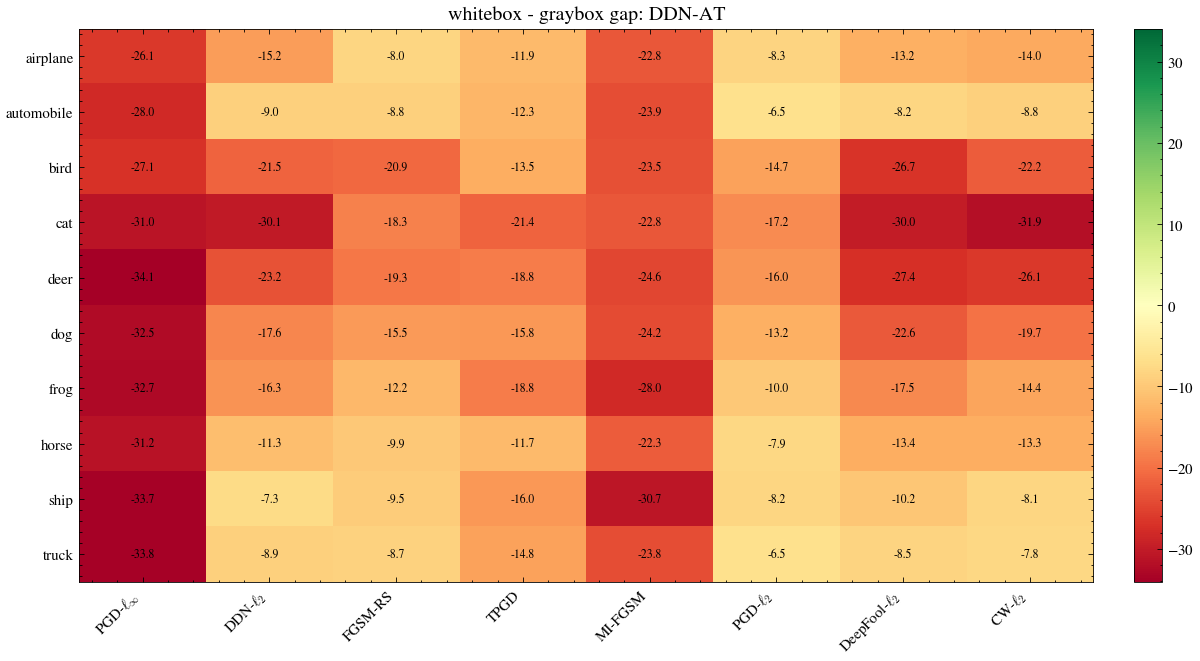
\includegraphics[width=\linewidth]{figures/graybox/whitebox_graybox_gap_DDNAT.png}
\caption{Whitebox--graybox gap heatmap for DDN-AT.}
\label{fig:ch6_graybox_gap_ddnat}
\end{figure}

\begin{figure}[H]
\centering
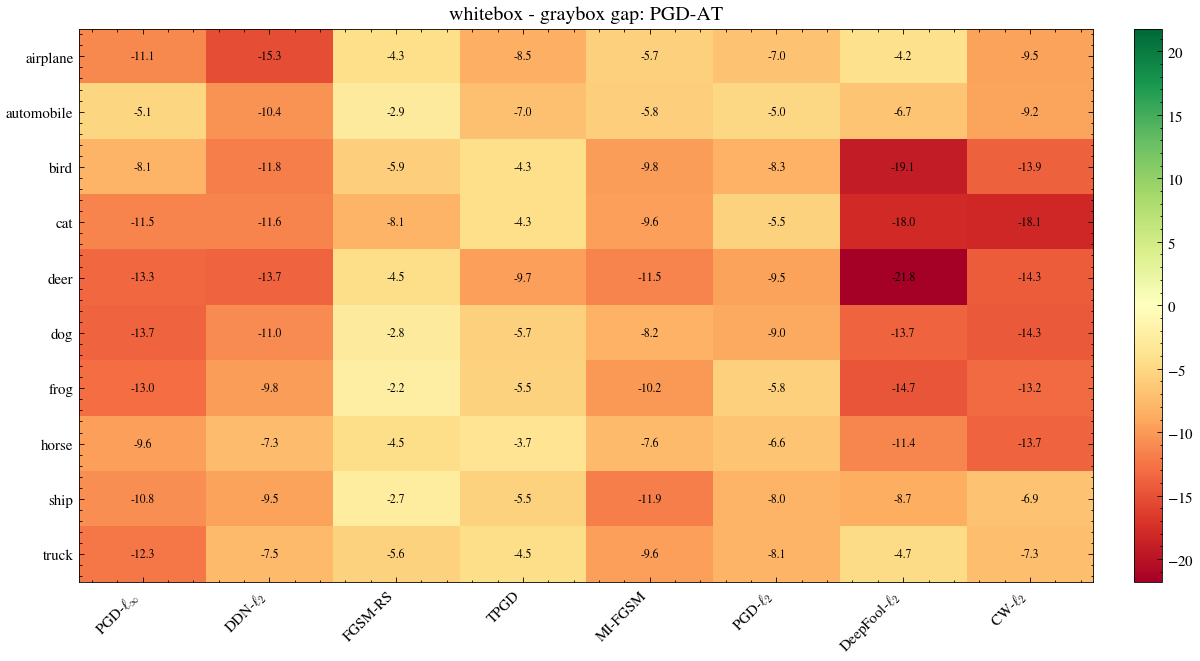
\includegraphics[width=\linewidth]{figures/graybox/whitebox_graybox_gap_PGDAT.png}
\caption{Whitebox--graybox gap heatmap for PGD-AT.}
\label{fig:ch6_graybox_gap_pgdat}
\end{figure}

\begin{figure}[H]
\centering
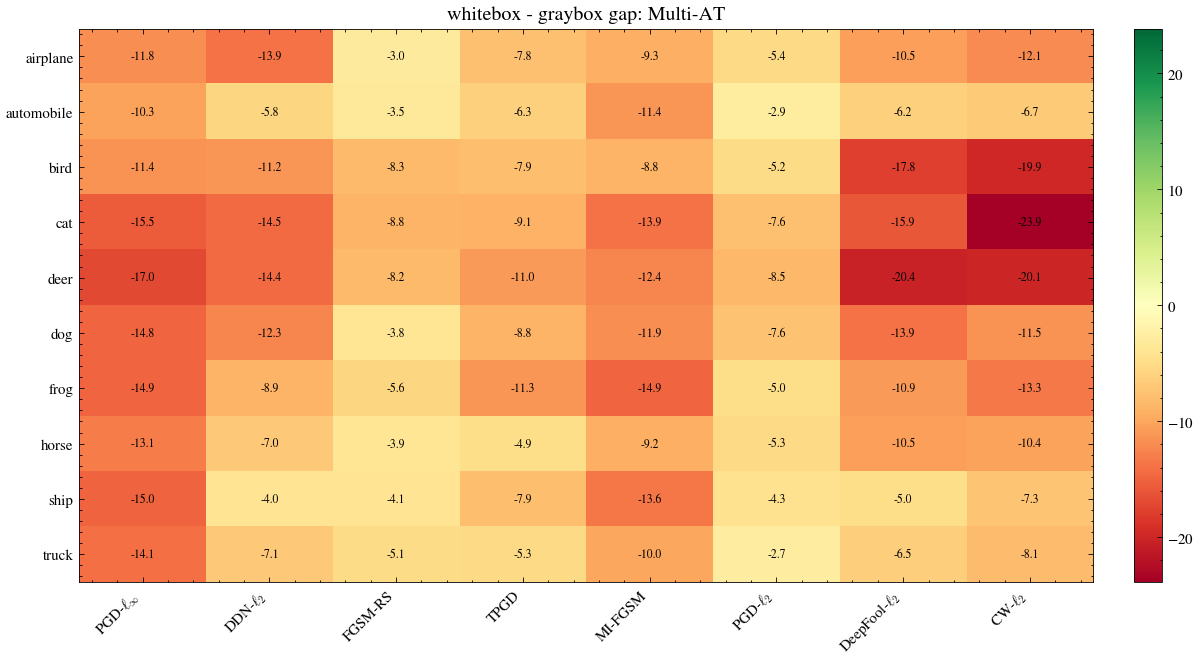
\includegraphics[width=\linewidth]{figures/graybox/whitebox_graybox_gap_MultiAT.png}
\caption{Whitebox--graybox gap heatmap for Multi-AT.}
\label{fig:ch6_graybox_gap_multiat}
\end{figure}

\begin{figure}[H]
\centering
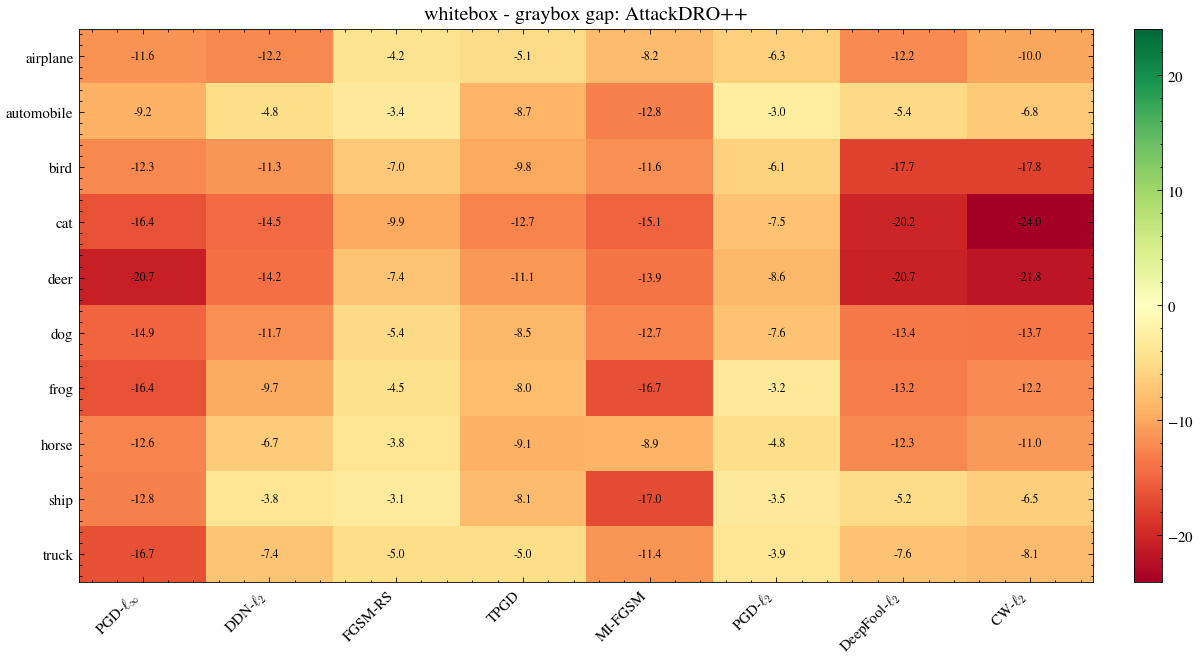
\includegraphics[width=\linewidth]{figures/graybox/whitebox_graybox_gap_AttackDROpp.png}
\caption{Whitebox--graybox gap heatmap for AttackDRO++ (Ours).}
\label{fig:ch6_graybox_gap_attackdropp}
\end{figure}

DDN-AT exhibits broad positive gaps on the \(\ell_\infty\)-oriented
attack columns, indicating that its high graybox score is partly driven
by weak transfer from \(\ell_\infty\) surrogates rather than uniformly
strong robustness. PGD-AT, Multi-AT, and AttackDRO++ show smaller and
more balanced gap patterns, with AttackDRO++ avoiding the severe
specialist inflation observed for DDN-AT.
\subsection{Class-Level Transfer Patterns}
\label{subsec:ch6_class_level_transfer_patterns}

% TODO[Kiệt]:
% Goal:
% - Explain fine-grained graybox gains and failures by class and attack.
% Flow:
% - Interpret `tab:ch6_graybox_per_cell`, then use delta heatmaps to show where gains concentrate.
% Include:
% - Reference `fig:ch6_graybox_delta_multiat`, `fig:ch6_graybox_delta_pgdat`, and `fig:ch6_graybox_delta_ddnat` if all remain in the main flow.
% Avoid:
% - Listing every class-attack cell.
% Target length: 3-5 paragraphs.

We complement the aggregate analysis with a paired per-cell test. For
each of the $80$ attack--class cells, we compare the graybox accuracy of
the AttackDRO++ target against each baseline target across the five
training seeds (each cell pairs $n = 5$ seeds). A two-sided paired
$t$-test is computed per cell.

\begin{table}[H]
\centering
\caption{Per-(class \(\times\) attack) graybox tests comparing
AttackDRO++ against each baseline. \(\Delta\) is computed as
AttackDRO++ minus the baseline.}
\label{tab:ch6_graybox_per_cell}
\footnotesize
\setlength{\tabcolsep}{4.5pt}
\renewcommand{\arraystretch}{1.18}
\begin{tabular}{lccccc}
\toprule
Baseline
& Positive cells
& Sign-test
& Mean
& Significant cells
& Bottom-10 \\
& \((\Delta>0)\)
& \(p\)
& \(\Delta\) (pp)
& AttackDRO++ / Baseline
& lift (pp) \\
\midrule
Multi-AT
& $59/80$
& $\mathbf{1.3{\times}10^{-5}}$
& $+0.557$
& $\phantom{0}2 \,/\, \phantom{0}3$
& $+0.779$ \\

PGD-AT
& $52/80$
& $\mathbf{4.8{\times}10^{-3}}$
& $+2.332$
& $34 \,/\, 12$
& $+1.329$ \\

DDN-AT
& $27/80$
& $\mathbf{2.4{\times}10^{-3}}$
& $-2.206$
& $16 \,/\, 32$
& $+0.709$ \\
\bottomrule
\end{tabular}
\end{table}

Three observations follow. First, AttackDRO++ exceeds Multi-AT on
$59$ of $80$ cells with a mean per-cell delta of $+0.557$~pp, in close
agreement with the $+0.549$~pp aggregate from
Table~\ref{tab:ch6_paired_graybox_two_panel}. Cell-level significance is sparse
($2$ vs.\ $3$ cells reach $p < 0.05$ in either direction), as expected
under the $n = 5$ per-cell sample size and the small absolute deltas;
the bulk of the evidence for AttackDRO++ is therefore the
\emph{distributional} shift across many cells rather than a few cell-level
landslides.

Second, the bottom-10 lift is positive in all three contrasts. The cells
on which Multi-AT, PGD-AT, and DDN-AT are weakest concentrate on
the cat, deer, dog, and bird classes under MI-FGSM, PGD-$\ell_\infty$,
and PGD-$\ell_2$. AttackDRO++ improves on Multi-AT by
$+0.779$~pp on Multi-AT's worst $10$ cells, and improves on
PGD-AT by $+1.329$~pp on PGD-AT's worst $10$ cells.

Third, the AttackDRO++ vs.\ DDN-AT cell-level comparison ($-2.21$~pp on
average, $32$ cells favoring DDN-AT at $p<0.05$) is the per-cell
counterpart of the DDN-AT graybox inflation: most of DDN-AT's wins are
on $\ell_2$ cells, while AttackDRO++ retains the wins it needs on the
$\ell_\infty$ cells that DDN-AT collapses on under whitebox attack
(Section~\ref{subsec:ch6_per_attack_accuracy}).

The heatmaps in
Figures~\ref{fig:ch6_graybox_delta_multiat}--\ref{fig:ch6_graybox_delta_ddnat} visualize these patterns
explicitly: green cells favor AttackDRO++, red cells favor the baseline.
The AttackDRO++ vs.\ Multi-AT heatmap is broadly green and small
in magnitude; the AttackDRO++ vs.\ PGD-AT heatmap is broadly green with
a few large red cells on $\ell_\infty$ attacks where PGD-AT specializes;
and the AttackDRO++ vs.\ DDN-AT heatmap is mixed.

\begin{figure}[H]
\centering
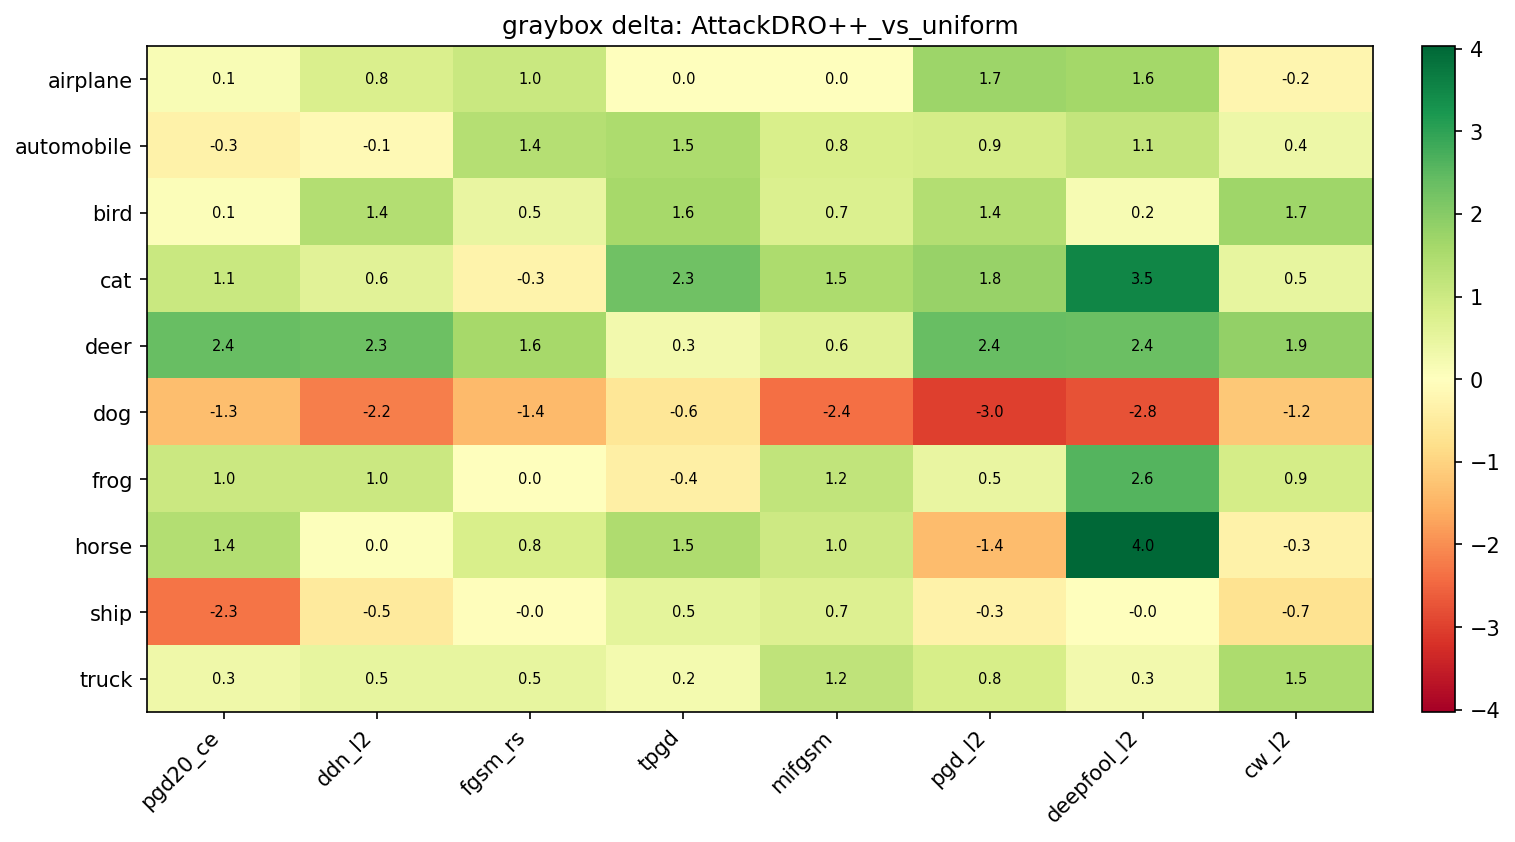
\includegraphics[width=\linewidth]{figures/graybox/graybox_delta_per_class_attack_AttackDRO++_vs_uniform.png}
\caption{Per-(class \(\times\) attack) graybox delta heatmap for
AttackDRO++ (Ours) minus Multi-AT. Green favors AttackDRO++ (Ours); red favors
Multi-AT.}
\label{fig:ch6_graybox_delta_multiat}
\end{figure}

\begin{figure}[H]
\centering
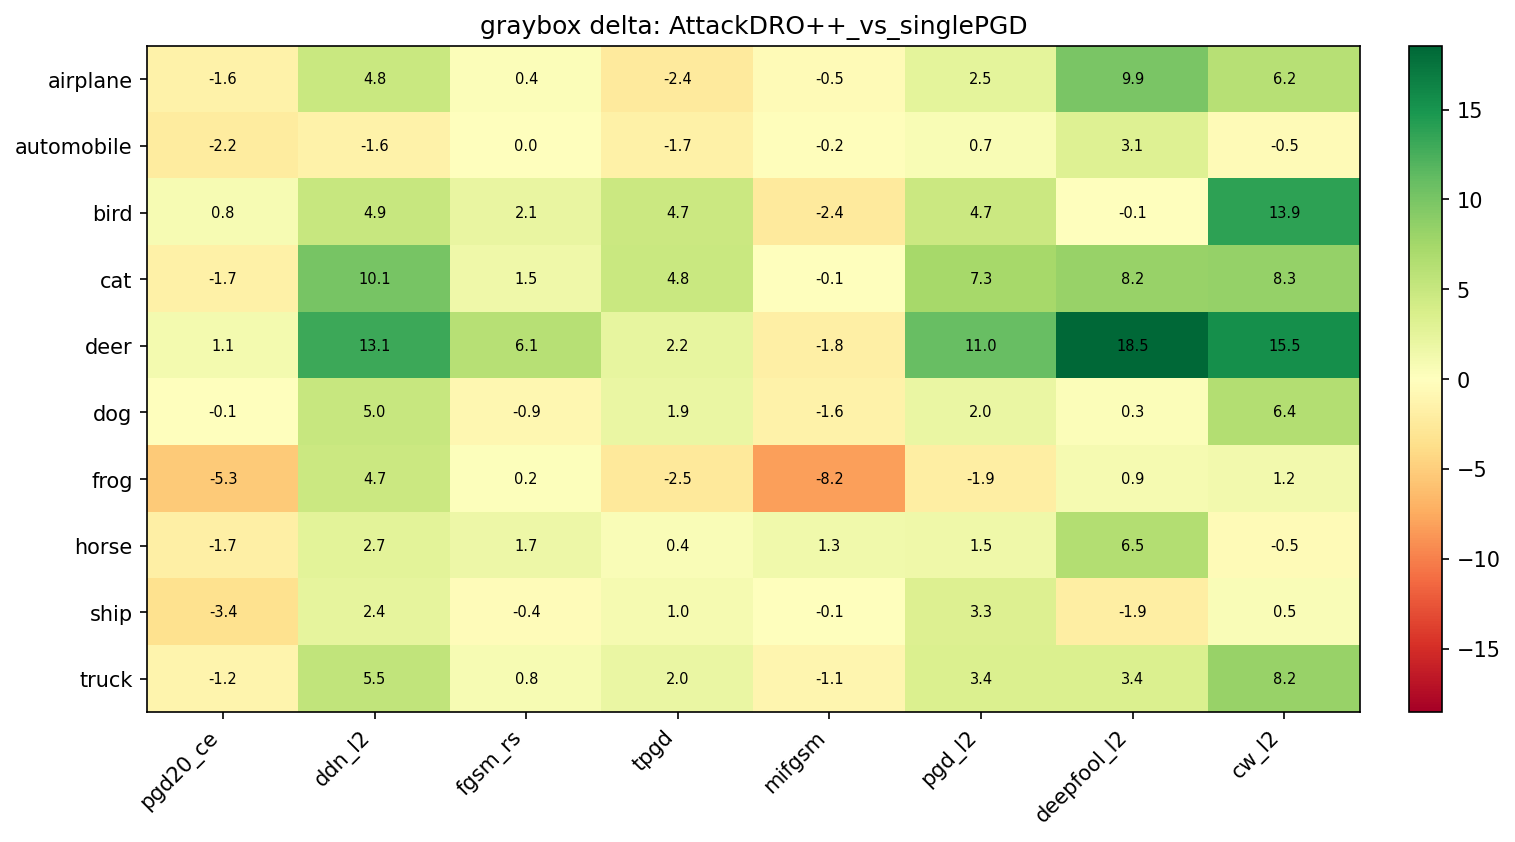
\includegraphics[width=\linewidth]{figures/graybox/graybox_delta_per_class_attack_AttackDRO++_vs_singlePGD.png}
\caption{Per-(class \(\times\) attack) graybox delta heatmap for
AttackDRO++ (Ours) minus PGD-AT. Green favors AttackDRO++ (Ours); red favors PGD-AT.}
\label{fig:ch6_graybox_delta_pgdat}
\end{figure}

\begin{figure}[H]
\centering
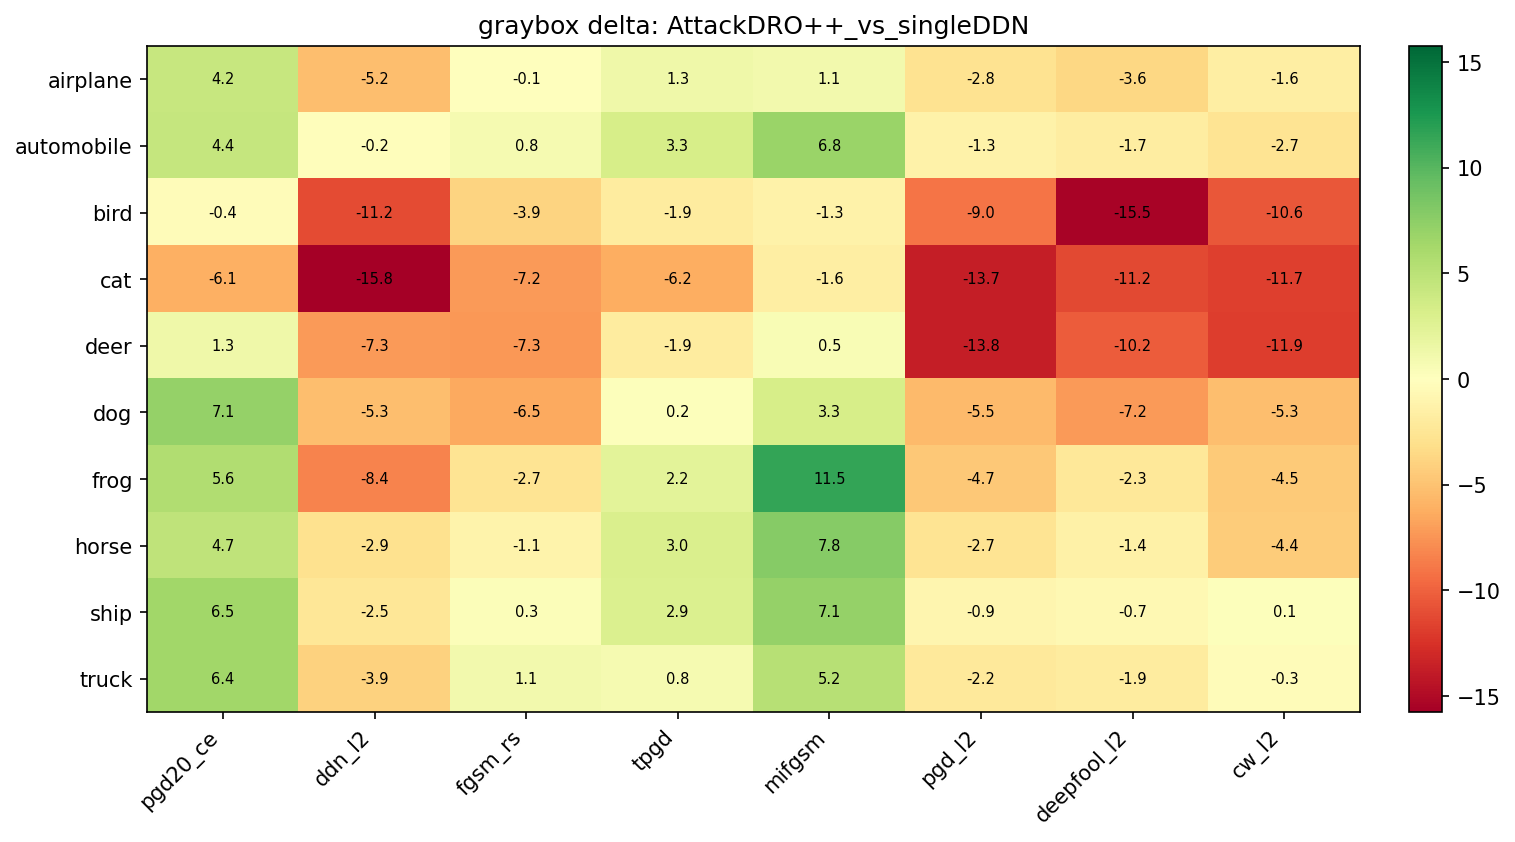
\includegraphics[width=\linewidth]{figures/graybox/graybox_delta_per_class_attack_AttackDRO++_vs_singleDDN.png}
\caption{Per-(class \(\times\) attack) graybox delta heatmap for
AttackDRO++ (Ours) minus DDN-AT. Green favors AttackDRO++ (Ours); red favors DDN-AT.}
\label{fig:ch6_graybox_delta_ddnat}
\end{figure}

\newpage
\paragraph{Method contribution decomposition.}

% TODO[Kiệt]:
% Goal:
% - Explain the contribution split between multi-attack training and Cluster-DRO components.
% Flow:
% - Interpret the decomposition table first, then use the figure as visual support.
% Include:
% - Reference `tab:ch6_graybox_decomposition` and `fig:ch6_method_decomposition` if kept.
% Avoid:
% - Treating decomposition as causal proof beyond the available comparisons.
% Target length: 2-4 paragraphs.

The whitebox results of Section~\ref{sec:ch6_whitebox} compare AttackDRO++
against Multi-AT and against the two single-attack baselines as
three separate contrasts. Under graybox transfer, we can additionally
ask how much of the AttackDRO++ improvement over each single-attack
baseline is contributed by multi-attack training (the Multi-AT
component) versus the Cluster-DRO objective (the AttackDRO++ component
on top of Multi-AT). We decompose the total
AttackDRO++ vs.\ single-attack delta as
\[
\Delta_{\text{total}}
\;=\;
\underbrace{(\text{Multi-AT}) - (\text{single-AT})}_{\Delta_{\text{multi-attack}}}
\;+\;
\underbrace{(\text{AttackDRO++}) - (\text{Multi-AT})}_{\Delta_{\text{Cluster-DRO}}},
\]
and report this decomposition for whitebox Mean(8), cross-method graybox
Mean(8), and the bottom-10-cell cross-method graybox average (the average
graybox accuracy on the ten attack--class cells in which the target is
weakest). The bottom-10 metric is included because it isolates worst-cell
behavior, which is most sensitive to the AttackDRO++ objective.

\begin{table}[H]
\centering
\caption{AttackDRO++ (Ours) gain decomposition. Values are percentage-point changes.}
\label{tab:ch6_graybox_decomposition}
\small
\setlength{\tabcolsep}{6pt}
\renewcommand{\arraystretch}{1.10}
\begin{tabular}{llrrr}
\toprule
Metric & Base & Multi-AT & DRO++ & Total \\
\midrule
Whitebox Mean(8)        & PGD-AT & $+0.934$ & $+0.184$ & $+1.118$ \\
Whitebox Mean(8)        & DDN-AT & $+5.536$ & $+0.184$ & $+5.720$ \\
\midrule
Cross-graybox Mean(8)   & PGD-AT & $+1.775$ & $+0.557$ & $+2.332$ \\
Cross-graybox Mean(8)   & DDN-AT & $-2.763$ & $+0.557$ & $-2.206$ \\
\midrule
Bottom-10 graybox       & PGD-AT & $+0.530$ & $+0.799$ & $+1.329$ \\
Bottom-10 graybox       & DDN-AT & $-0.090$ & $+0.799$ & $+0.709$ \\
\bottomrule
\end{tabular}
\end{table}
The Cluster-DRO effect (column 4) is positive on every metric and
decomposition path, ranging from $+0.184$~pp on whitebox Mean(8) to
$+0.799$~pp on the bottom-10 cross-graybox metric. Two implications
follow. First, the Cluster-DRO effect is larger under graybox transfer
than under direct whitebox attack, consistent with the
$+0.279$~pp $\rightarrow$ $+0.549$~pp scaling observed in
Section~\ref{subsec:ch6_paired_graybox_comparisons}. Second, the Cluster-DRO effect is
roughly four times larger on the bottom-10 cells ($+0.799$~pp) than on
whitebox Mean(8), supporting the design intent that the Cluster-DRO
objective primarily reshapes worst-cell behavior rather than the
average.

The multi-attack column tells a complementary specialist story. Going
from single-AT to Multi-AT adds $+5.54$~pp of whitebox Mean(8)
when the baseline is DDN-AT, but removes $-2.76$~pp of cross-graybox
Mean(8) for the same baseline --- because DDN-AT's graybox accuracy is
inflated by the very $\ell_\infty$ transfer mismatch that
Multi-AT corrects. The cluster-DRO component remains positive in both
cases, indicating that it adds robustness that is not absorbed by either
multi-attack training alone or DDN-AT's structural graybox advantage.

\begin{figure}[H]
\centering
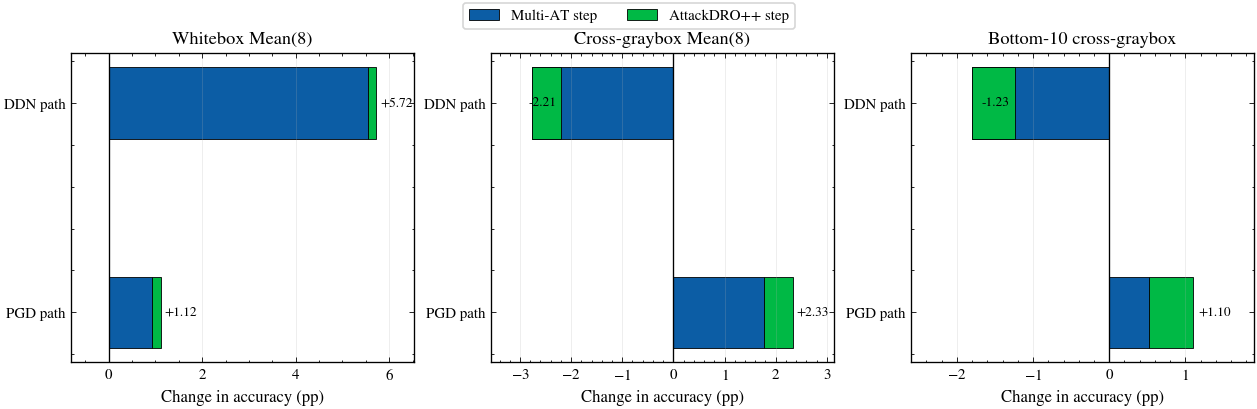
\includegraphics[width=\linewidth]{figures/graybox/method_decomposition_three_panel_science.png}
\caption{Visual decomposition of AttackDRO++ improvement over the
single-attack baselines into a multi-attack effect (Multi-AT
minus single-AT) and a Cluster-DRO effect (AttackDRO++ minus Multi-AT) across whitebox, cross-method graybox, and bottom-10
cross-method graybox metrics, for the two single-AT decomposition
paths.}
\label{fig:ch6_method_decomposition}
\end{figure}

% Section summary removed; transition/closing prose should be written later.
\iffalse
% Disabled graybox section summary removed from the numbered structure.

% TODO[Kiệt]:
% Goal:
% - Remove or convert this section-level summary in a later style cleanup.
% Flow:
% - Replace with a short transition paragraph or move synthesis into `6_summary.tex`.
% Include:
% - No new results.
% Avoid:
% - Keeping section-level summaries against docs/06_style_rules.md.
% Target length: 0 paragraphs here after cleanup; use Chapter 6 summary instead.

The graybox transfer results jointly establish the following
conclusions:

\begin{enumerate}
  \item The graybox random-seed checkpoint panel preserves the whitebox
        trend: it reproduces the Mean(8) ranking AttackDRO++ $>$ Multi-AT
        $>$ PGD-AT $>$ DDN-AT to within $1.0$~pp.
  \item AttackDRO++ improves on Multi-AT by $+0.549$~pp under
        symmetric cross-method graybox transfer at $p \approx 1.1
        \times 10^{-8}$ ($d_z = 0.42$, $n=200$), roughly twice the
        whitebox delta on the same panel. The Cluster-DRO improvement
        therefore strengthens rather than disappears under transfer.
  \item The graybox gain is broad: AttackDRO++ produces a positive
        per-attack delta against Multi-AT on all eight
        evaluation attacks, with five attacks individually significant
        at $p<0.05$ and the largest gain on DeepFool-$\ell_2$
        ($+1.47$~pp, $p<10^{-3}$). It is the only method that meets or
        exceeds Multi-AT on every attack family.
  \item DDN-AT's row-leading graybox accuracy is structural rather
        than substantive.. Its whitebox--graybox gap is $+18.20$~pp,
        roughly twice that of every other method, because $\ell_\infty$
        adversarial examples generated by alternative surrogates
        transfer poorly to a purely-$\ell_2$-trained target. The strong
        graybox row should not be confused with broader robustness;
        DDN-AT's whitebox Mean(8) and Worst(8) remain the lowest of
        the four methods.
  \item The per-cell drilldown shows that AttackDRO++ exceeds        Multi-AT on $59$ of $80$ attack--class cells, with a bottom-10
        lift of $+0.779$~pp on Multi-AT's weakest cells. The
        Cluster-DRO contribution decomposes as approximately $+0.18$~pp
        on whitebox Mean(8), $+0.56$~pp on cross-graybox Mean(8), and
        $+0.80$~pp on the bottom-10 cross-graybox metric, supporting
        the design intent that the objective primarily reshapes
        worst-cell behavior.
\end{enumerate}

These graybox results corroborate the whitebox conclusions of
Section~\ref{sec:ch6_whitebox}: the AttackDRO++ improvement over
Multi-AT reflects a broader cross-attack robustness profile, not a
defense narrowly tuned to its own gradients. The single-attack baselines
remain specialists under both whitebox and graybox attack, and DDN-AT's
apparent graybox strength is exposed as a transfer-mismatch artefact by
the whitebox--graybox gap analysis. The next section examines how these
behaviors emerge during training.
\fi

\section{Sensitivity to Key Hyperparameters}
\label{sec:ch6_ablation}

The preceding sections evaluated the final AttackDRO++ configuration under
whitebox, class-wise, and graybox settings. Those results show how the method
behaves once the design choices are fixed, but they do not explain how sensitive
the method is to those choices. This section therefore studies three practical
hyperparameters: the number of discovered clusters, the strength of the uniform
anchor, and the frequency with which clusters are refreshed.

These ablations are intended as configuration guidance rather than as a second
main comparison. Unless otherwise stated, they use the same CIFAR-10, ResNet-18,
source-attack, and evaluation-attack protocol defined in Chapter~\ref{chap:experimental_setup}.
Mean(8) and Worst(8) follow the definitions in Section~\ref{sec:ch5_evaluation_metrics}:
both are computed over the eight non-AutoAttack evaluation attacks, while
AutoAttack-$\ell_\infty$ is reported separately.

\subsection{Number of Clusters: How Many Groups Are Needed?}
\label{subsec:ch6_ablation_num_clusters}

The number of clusters controls the granularity of the latent groups used by
AttackDRO++. If $K$ is too small, distinct failure modes may be merged into the
same group, making the Cluster-DRO correction too coarse. If $K$ is too large,
the minibatch may be split into many small groups, making group-loss estimates
noisier and the cluster weights less stable.

Because $K$ controls the trade-off between coarse grouping and noisy small groups,
Table~\ref{tab:ch6_ablation_num_clusters} tests whether AttackDRO++ is sensitive to
cluster granularity. Across the available runs, all settings remain close in Mean(8), with differences
well below one percentage point. The default $K=4$ setting gives the highest
Worst(8) among the tested settings and remains competitive in Mean(8), while
$K=2$ is slightly more coarse and $K=6$ or $K=10$ do not provide a clear gain.
The $K=10$ setting uses only two valid runs and should be interpreted
as weaker evidence than the other cluster-count settings.

\begin{table}[H]
\centering
\caption{Number-of-clusters ablation for AttackDRO++ with anchor strength
$\lambda_{\mathrm{DRO}}=0.35$. Values are robust accuracy (\%) reported as
mean $\pm$ standard deviation across available runs. Mean(8) and Worst(8) are
computed over the eight non-AutoAttack attacks; AutoAttack-$\ell_\infty$ is
reported separately. Bold values indicate the best setting for each metric.}
\label{tab:ch6_ablation_num_clusters}
\small
\setlength{\tabcolsep}{4pt}
\renewcommand{\arraystretch}{1.08}
\begin{tabular}{lccccc}
\toprule
Setting & $K$ & Runs & Mean(8) $\uparrow$ & Worst(8) $\uparrow$ & AutoAttack $\uparrow$ \\
\midrule
Coarse grouping
& 2 & 3
& $62.33 \pm 0.06$
& $45.13 \pm 0.27$
& $40.95 \pm 0.90$ \\

Default grouping
& 4 & 3
& \bestval{62.35 $\pm$ 0.20}
& \bestval{45.33 $\pm$ 0.25}
& \bestval{41.14 $\pm$ 1.15} \\

Finer grouping
& 6 & 3
& $62.28 \pm 0.14$
& $45.17 \pm 0.47$
& $40.95 \pm 1.30$ \\

Very fine grouping
& 10 & 2
& $62.35 \pm 0.09$
& $45.17 \pm 0.08$
& $40.62 \pm 1.11$ \\
\bottomrule
\end{tabular}
\end{table}

\begin{figure}[H]
    \centering
    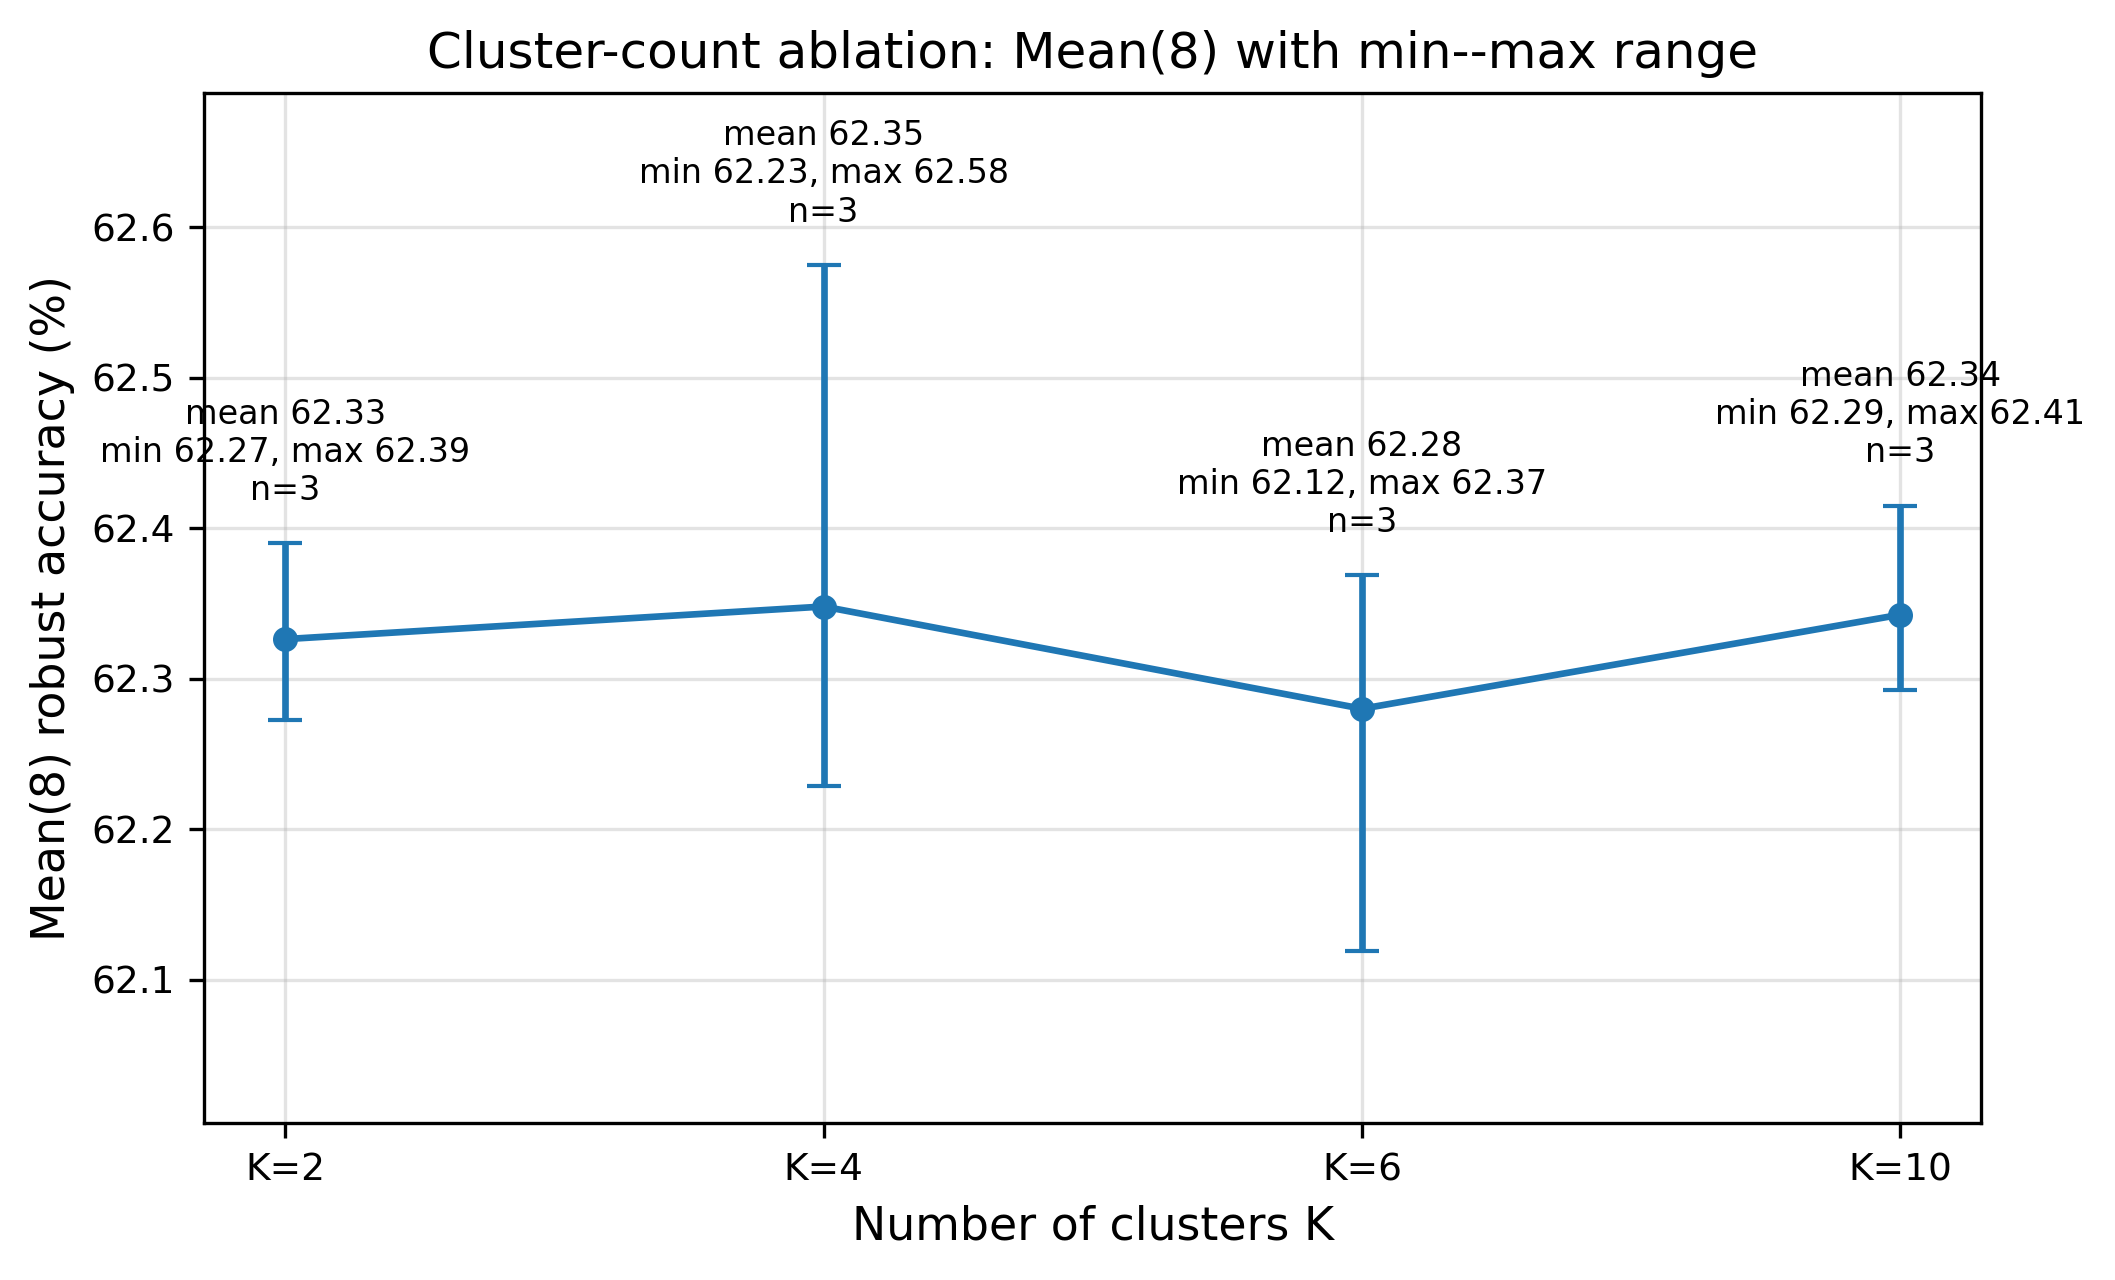
\includegraphics[width=0.82\linewidth]{figures/ablations/ablation_num_clusters.png}
    \caption{Sensitivity of AttackDRO++ to the number of clusters. Points show Mean(8) robust accuracy with the min-to-max range across available runs; Mean(8) is computed over the eight non-AutoAttack evaluation attacks.}
    \label{fig:ch6_ablation_num_clusters}
\end{figure}

The ablation supports using a moderate number of clusters rather than treating
the cluster count as a highly tuned parameter. The default $K=4$ is expressive
enough to go beyond the two source attack identities, but it does not fragment
the training batch as aggressively as larger values. Therefore, the evidence
supports $K=4$ as a stable practical choice, not as a universally optimal cluster
count.

\subsection{Anchor Strength: Finding a Stable Trade-off}
\label{subsec:ch6_ablation_anchor_strength}

The anchor strength $\lambda_{\mathrm{DRO}}$ controls the interpolation between
the uniform multi-attack ERM objective and the adaptive Cluster-DRO objective.
A smaller value keeps training closer to the uniform baseline, while a larger
value gives the cluster-reweighted loss more influence. In this ablation, the
previous $\lambda_{\mathrm{DRO}}=1.0$ setting is removed because it corresponds
to an overly aggressive Cluster-DRO setting and is not part of the final
candidate set.

Because the anchor controls how far the objective can move away from uniform Multi-AT,
Table~\ref{tab:ch6_ablation_anchor_strength} tests three practical anchor strengths.
The differences are again small, but the moderate setting
$\lambda_{\mathrm{DRO}}=0.35$ gives the strongest Mean(8), Worst(8), and
AutoAttack values among the tested settings. The lower value
$\lambda_{\mathrm{DRO}}=0.20$ remains close, suggesting that the method does not
require a sharply tuned anchor. The higher value $\lambda_{\mathrm{DRO}}=0.50$
slightly reduces Mean(8) and AutoAttack, which is consistent with the idea that
too much emphasis on adaptive cluster weighting can reduce the stabilizing effect
of the uniform multi-attack baseline.

\begin{table}[H]
\centering
\caption{Anchor-strength ablation for AttackDRO++ with $K=4$. Values are robust
accuracy (\%) reported as mean $\pm$ standard deviation across three runs.
Mean(8) and Worst(8) are computed over the eight non-AutoAttack attacks;
AutoAttack-$\ell_\infty$ is reported separately. Bold values indicate the best setting for each metric.}
\label{tab:ch6_ablation_anchor_strength}
\small
\setlength{\tabcolsep}{4pt}
\renewcommand{\arraystretch}{1.08}
\begin{tabular}{lcccc}
\toprule
Anchor strength $\lambda_{\mathrm{DRO}}$ & Runs & Mean(8) $\uparrow$ & Worst(8) $\uparrow$ & AutoAttack $\uparrow$ \\
\midrule
$0.20$
& 3
& $62.28 \pm 0.09$
& $45.01 \pm 0.40$
& $41.08 \pm 1.66$ \\

$0.35$ (default)
& 3
& \bestval{62.35 $\pm$ 0.20}
& \bestval{45.33 $\pm$ 0.25}
& \bestval{41.14 $\pm$ 1.15} \\

$0.50$
& 3
& $62.24 \pm 0.18$
& $45.24 \pm 0.40$
& $40.24 \pm 1.09$ \\
\bottomrule
\end{tabular}
\end{table}

\begin{figure}[H]
    \centering
    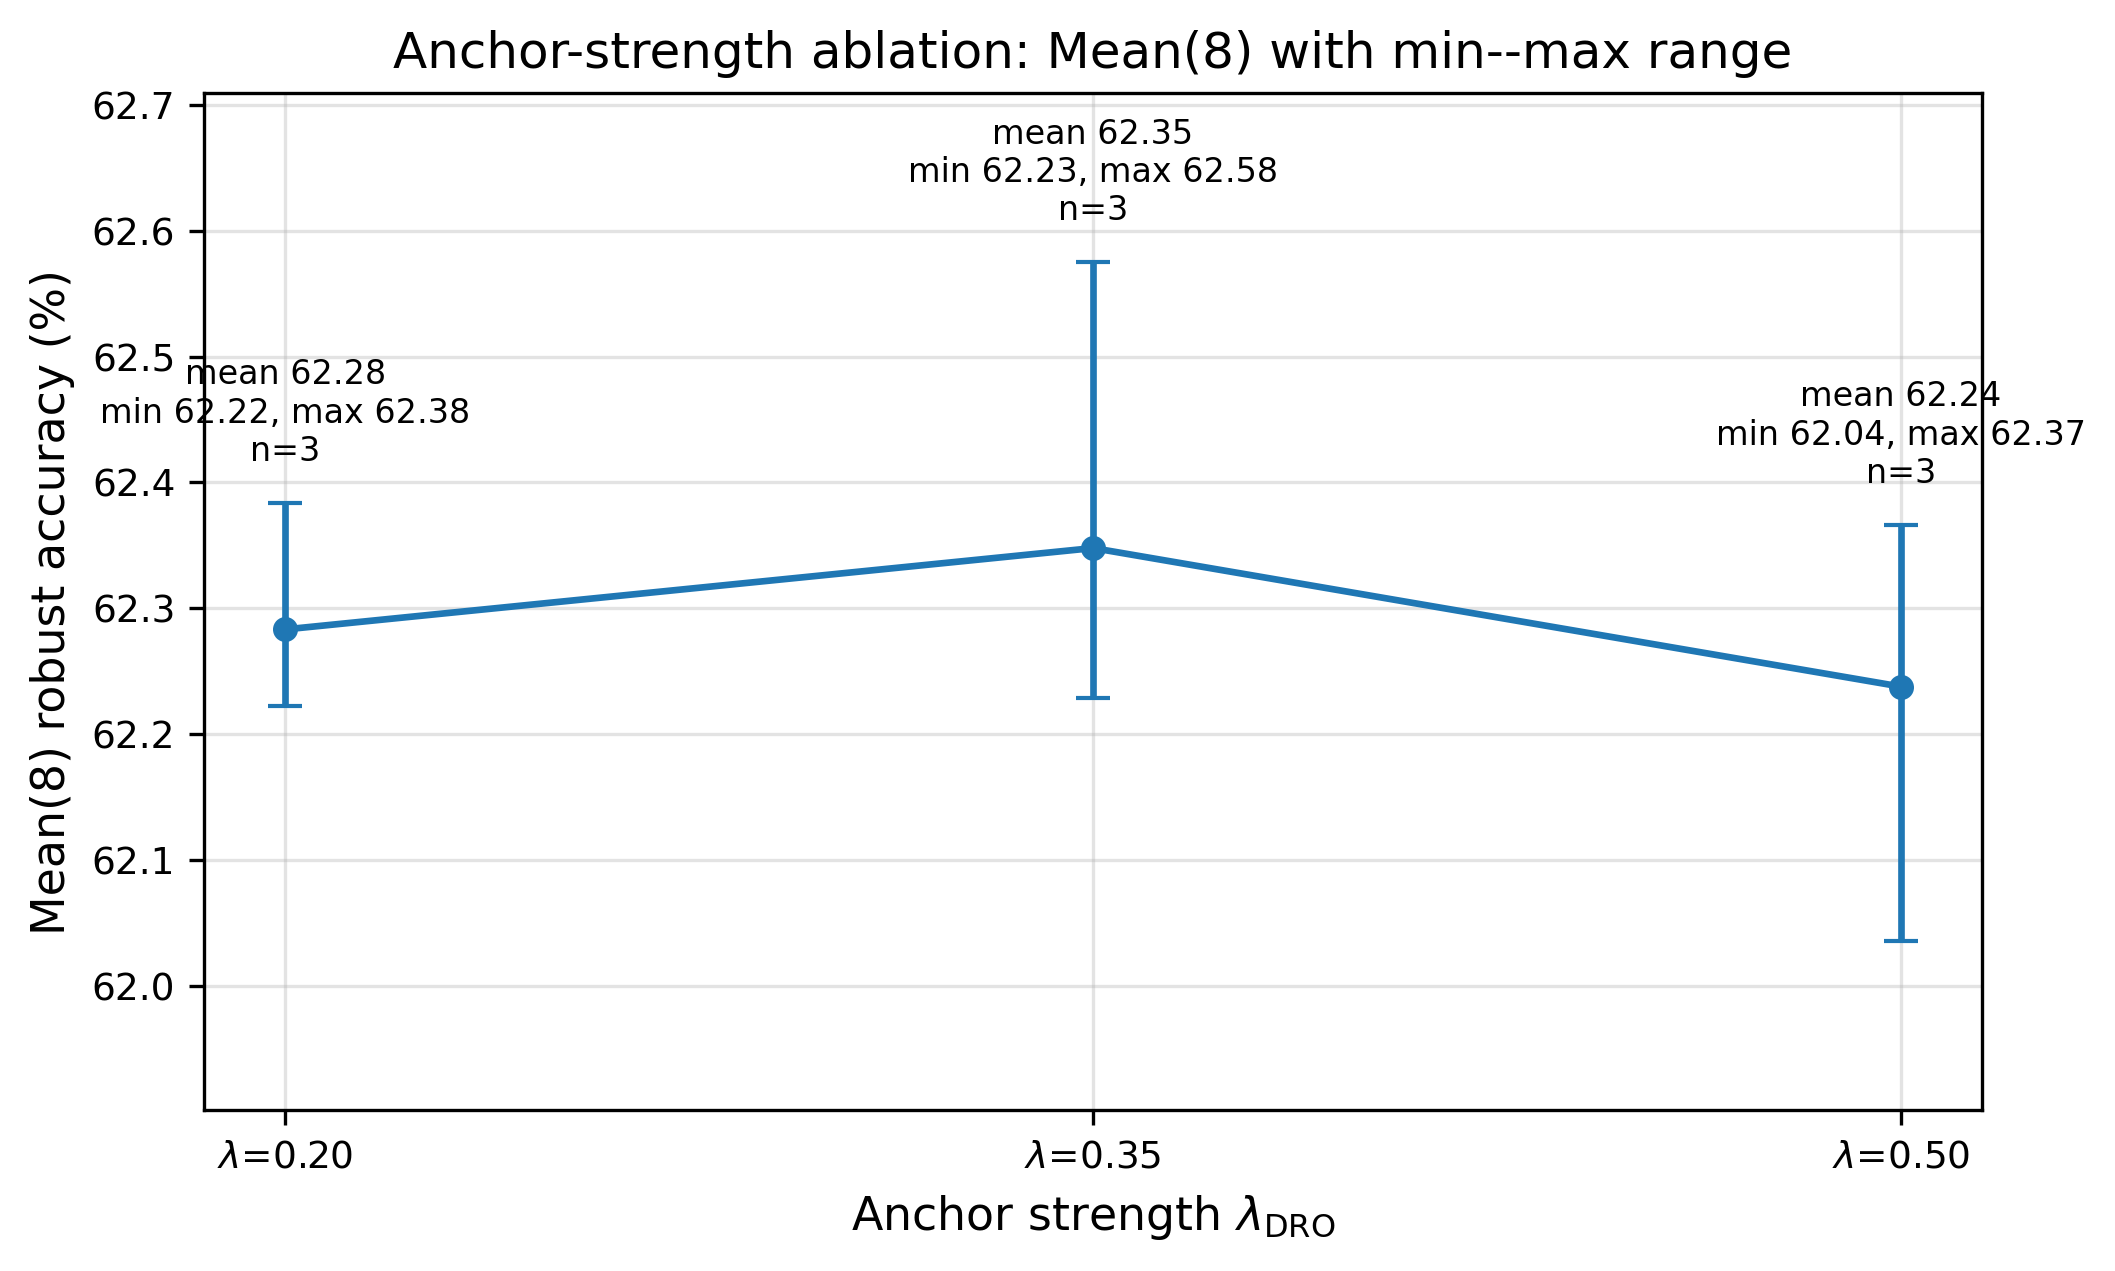
\includegraphics[width=0.82\linewidth]{figures/ablations/ablation_anchor_strength.png}
    \caption{Sensitivity of AttackDRO++ to the anchor strength $\lambda_{\mathrm{DRO}}$. Points show Mean(8) robust accuracy with the min-to-max range across available runs; Mean(8) is computed over the eight non-AutoAttack evaluation attacks. The previous $\lambda_{\mathrm{DRO}}=1.0$ setting is excluded from the final ablation panel.}
    \label{fig:ch6_ablation_anchor_strength}
\end{figure}

Overall, the anchor-strength ablation supports the design motivation from
Chapter~\ref{chap:methodology}. AttackDRO++ benefits from a nonzero
cluster-level correction, but the correction should remain anchored to the
uniform multi-attack objective. The default value
$\lambda_{\mathrm{DRO}}=0.35$ is retained because it gives the best balance
among the tested settings without relying entirely on either uniform ERM or
aggressive Cluster-DRO weighting.

\subsection{Recluster Frequency: How Often Should Groups Update?}
\label{subsec:ch6_ablation_recluster_frequency}

The cluster-refresh interval $R$ controls how often the K-means clusterer is
refitted from the feature bank. Refreshing every epoch may adapt faster to
changes in the representation, but it also changes the group structure more
frequently. Refreshing less often may give a more stable grouping signal, but it
may lag behind the evolving model.

Since the refresh interval trades adaptation speed against group stability,
Table~\ref{tab:ch6_cluster_refresh_schedule_ablation} compares refreshing every
one epoch with refreshing every two epochs. The two schedules produce nearly
identical Mean(8), Worst(8), and family-level behavior. The default two-epoch
schedule gives a slightly higher Mean(8) and $\ell_\infty$-family average, while
the one-epoch schedule gives a slightly higher Worst(8), AutoAttack, and
$\ell_2$-family average. These differences are small relative to the
three-run setting, so the ablation does not show a strong advantage for either
schedule.

\begin{table}[H]
\centering
\caption{Cluster-refresh schedule ablation for AttackDRO++ with
$\lambda_{\mathrm{DRO}}=0.35$, gradient fingerprints, and $K=4$. Values are
robust accuracy (\%) reported as mean $\pm$ standard deviation across three
runs. Mean(8) and Worst(8) are computed over the eight non-AutoAttack attacks;
AutoAttack-$\ell_\infty$ is reported separately. Bold values indicate the best setting for each metric.}
\label{tab:ch6_cluster_refresh_schedule_ablation}
\scriptsize
\setlength{\tabcolsep}{4pt}
\renewcommand{\arraystretch}{1.08}
\resizebox{\textwidth}{!}{%
\begin{tabular}{lcccccc}
\toprule
Refresh interval
& Runs
& Mean(8) $\uparrow$
& Worst(8) $\uparrow$
& AutoAttack $\uparrow$
& $\ell_2$-family avg. $\uparrow$
& $\ell_\infty$-family avg. $\uparrow$ \\
\midrule
1 epoch
& 3
& $62.38 \pm 0.14$
& \bestval{45.17 $\pm$ 0.34}
& \bestval{40.30 $\pm$ 1.37}
& \bestval{67.57 $\pm$ 0.16}
& $57.18 \pm 0.27$ \\

2 epochs (default)
& 3
& \bestval{62.44 $\pm$ 0.22}
& $45.14 \pm 0.23$
& $39.45 \pm 0.68$
& $67.56 \pm 0.08$
& \bestval{57.31 $\pm$ 0.35} \\
\bottomrule
\end{tabular}}
\end{table}

\begin{figure}[H]
    \centering
    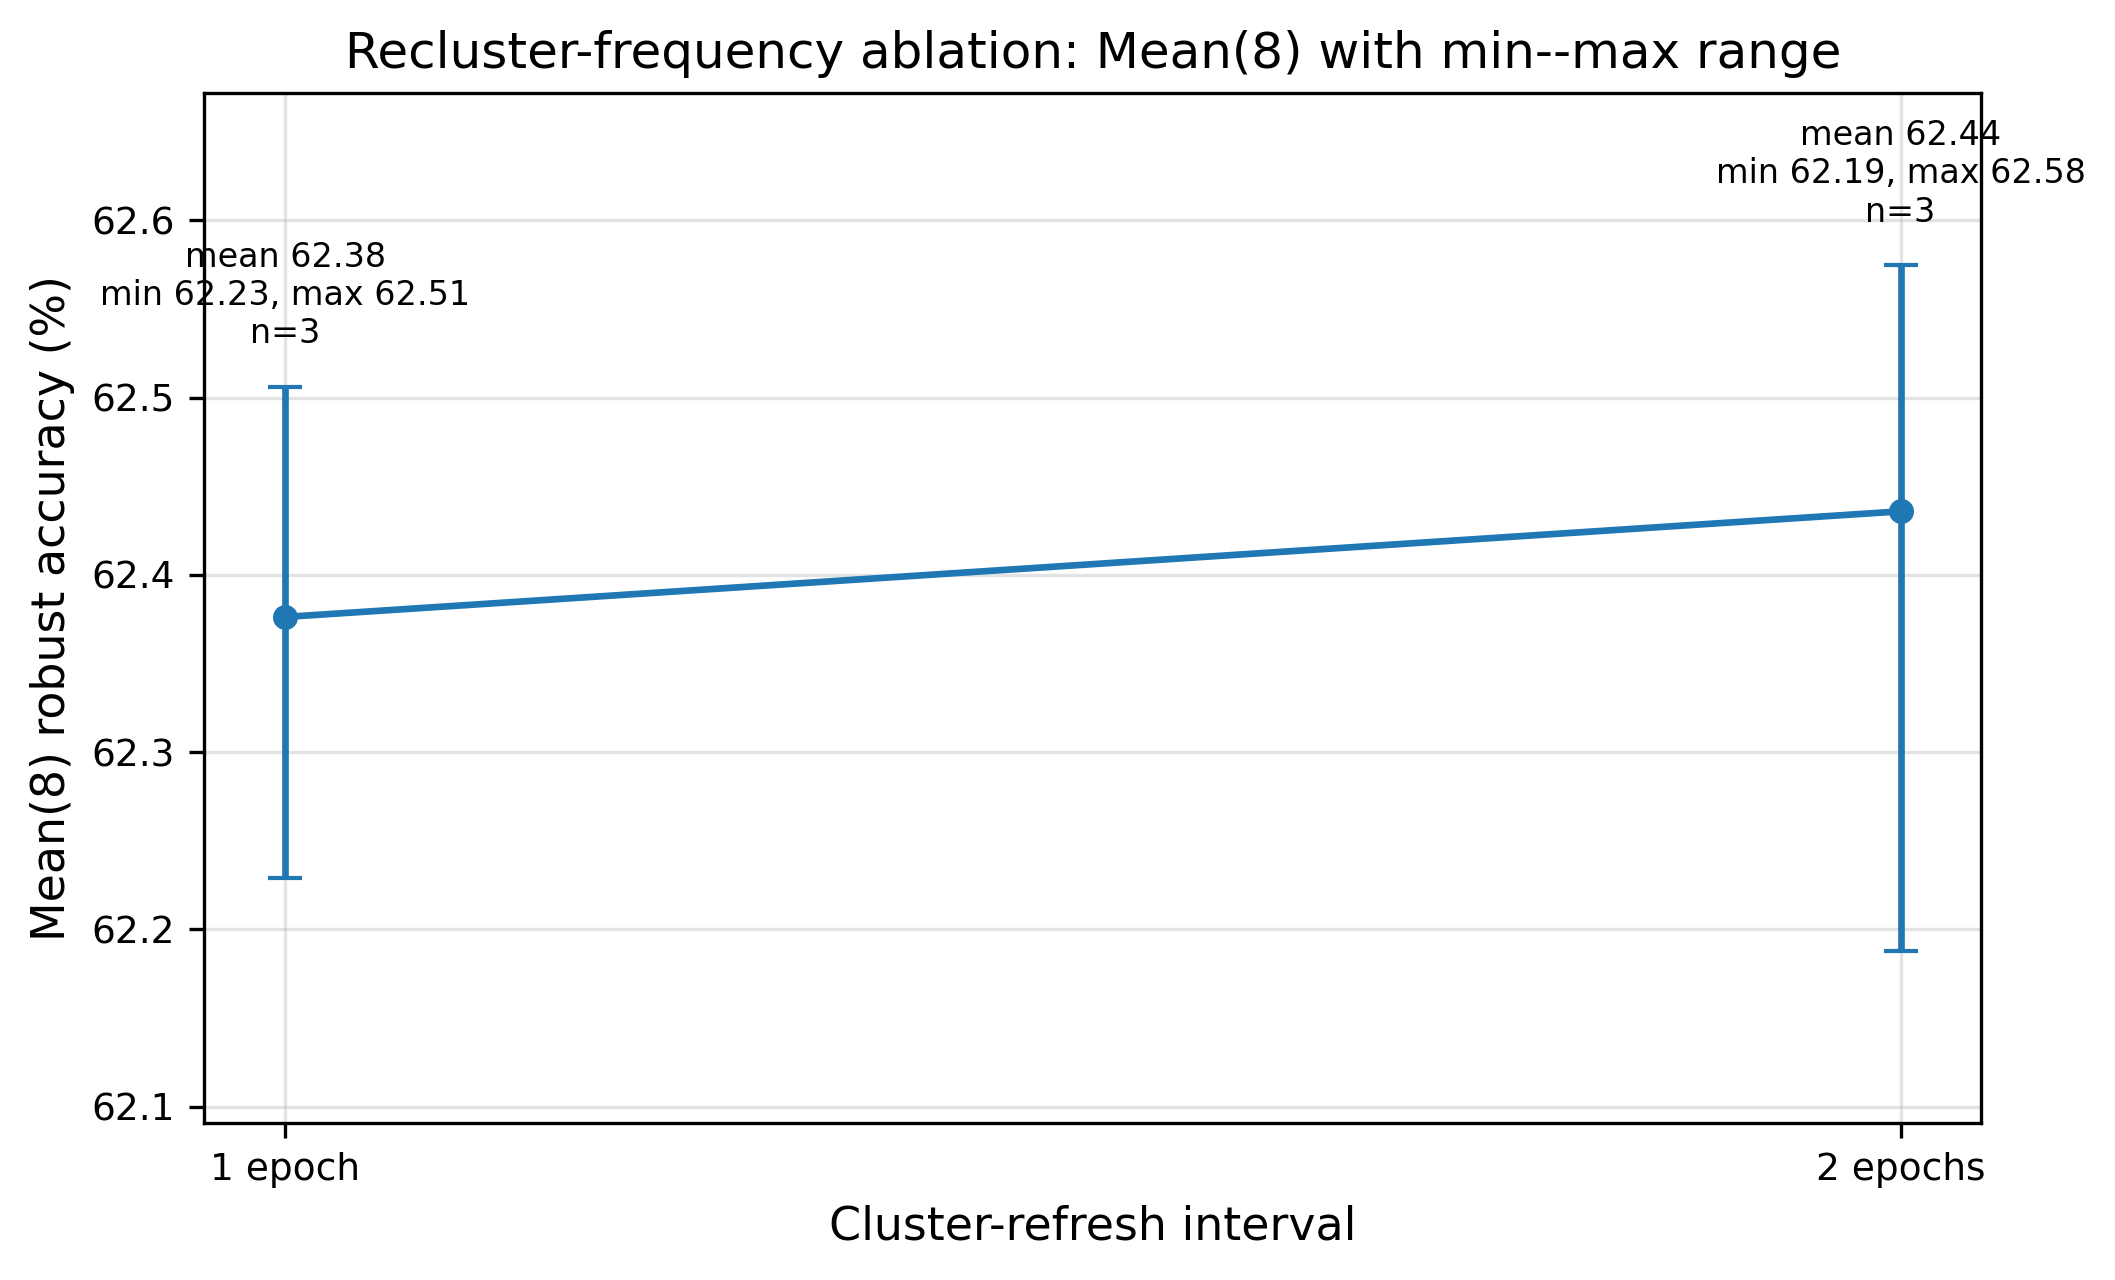
\includegraphics[width=0.82\linewidth]{figures/ablations/ablation_recluster_frequency.png}
    \caption{Sensitivity of AttackDRO++ to the cluster-refresh interval. Points show Mean(8) robust accuracy with the min-to-max range across available runs; Mean(8) is computed over the eight non-AutoAttack evaluation attacks. The two refresh schedules produce similar results, so the default two-epoch schedule is retained as a practical stability choice.}
    \label{fig:ch6_ablation_recluster_frequency}
\end{figure}

We retain $R=2$ epochs as the default because it gives comparable robustness
while reducing the frequency of cluster refitting. This is a practical choice:
the ablation suggests that the method is not highly sensitive to the exact
refresh interval, so the less frequent schedule is preferred for stability and
simplicity.

\paragraph{Supplementary architecture check.}
A single-run WRN-28-10 check is reported in Appendix~\ref{app:extras} as
supplementary evidence. This check is not included in the main paired claims
because it does not use the repeated-random-seed protocol of the main ResNet-18
experiments. In that setting, Multi-AT slightly outperforms AttackDRO++ on both
Mean(8) and AutoAttack-$\ell_\infty$, suggesting that the relative benefit of
the proposed grouping strategy may depend on model capacity and should be
evaluated more systematically in future work.

Together, these ablations suggest that the final AttackDRO++ configuration is
not the result of a fragile hyperparameter choice. Moderate clustering
granularity, moderate anchor strength, and a two-epoch refresh schedule provide a
stable practical configuration. The ablations also define the limits of the
current evidence: they support the selected ResNet-18 configuration, but broader
architecture-level conclusions require additional repeated-seed experiments.

% Diagnostics removed from main report outline; keep file for archive only.
% \section{Diagnostics}


\subsection{Embedding Visualization}

\subsection{Clustering Agreement}

\subsection{Cluster Composition Across Attacks and Classes}

\subsection{q Dynamics Across Training}     
Chapter~\ref{chap:results_analysis} evaluated AttackDRO++ through four connected
evidence panels. The aggregate whitebox results first showed that the proposed
method gives modest average and held-out gains relative to Multi-AT while
leaving Worst(8) and the separate AutoAttack checks broadly unchanged. The
per-attack and class-wise drilldowns then clarified where this behavior comes
from: the method acts less like a single-norm specialist and more like a
balanced multi-attack model, although hard animal-class cells under strong
\(\ell_\infty\) attacks remain persistent failure cases.

The graybox analysis tested whether the same pattern survives transferred
attacks from separately trained surrogate checkpoints. It supported the
whitebox interpretation while also showing that transfer accuracy must be read
carefully because specialist models can appear strong when attacks transfer
poorly across threat geometries. Finally, the ablation section examined whether
the observed behavior depends on key design choices, treating cluster count,
anchor strength, and refresh frequency as sensitivity checks rather than
standalone proof.

Overall, the supported conclusion is conservative: within the CIFAR-10 and
ResNet-18 setting studied here, AttackDRO++ improves cross-attack balance over
the uniform multi-attack baseline without establishing superiority on every
attack or extending robustness claims beyond the evaluated protocol. Chapter~\ref{chap:conclusion}
summarizes these findings, states the limitations, and outlines future
extensions.



% End of Chapter 6

\chapter{Conclusion and Future Work}
\label{chap:conclusion}

% TODO[Kiệt]:
% Goal:
% - Fill the empty conclusion shell with a compact final answer to the report's research questions.
% Flow:
% - Briefly restate the problem, answer each research question, summarize limitations, and propose future work.
% Include:
% - Consider a compact RQ answer table if it improves readability.
% - Mention limitations from dataset/model scope, attack suite, compute, and transfer protocol.
% Avoid:
% - New results, new citations, or a separate chapter summary section.
% Target length: 2-4 pages including optional RQ table.

\section{Summary of Contributions}

% TODO[Kiet]:
% Goal:
% - Restate the report contributions using evidence already presented in Chapter 6.
% Flow:
% - Problem framing -> method contribution -> evaluation contribution.
% Include:
% - Keep claims tied to the evaluated CIFAR-10/ResNet-18 setting.
% Avoid:
% - Introducing new result values or broader generalization claims.
% Target length: 3-5 paragraphs.

\section{Answers to Research Questions}

% TODO[Kiet]:
% Goal:
% - Answer each research question from Chapter 1 directly.
% Flow:
% - RQ -> concise answer -> evidence location in Chapter 6 -> limitation.
% Include:
% - Consider a compact RQ answer table.
% Avoid:
% - Repeating full result tables.
% Target length: 4-6 paragraphs or one compact table plus prose.

\section{Limitations of the Current Study}

% TODO[Kiet]:
% Goal:
% - State concrete boundaries of the current evidence.
% Flow:
% - Dataset/model scope -> attack suite scope -> compute/seed scope -> transfer protocol scope.
% Include:
% - Mention supplementary architecture evidence only if it is already in the report.
% Avoid:
% - Framing limitations as excuses or adding unsupported future claims.
% Target length: 3-5 paragraphs.

\section{Directions for Future Work}

% TODO[Kiet]:
% Goal:
% - Propose extensions that directly follow from the observed limitations.
% Flow:
% - Broader datasets/architectures -> stronger adaptive evaluation -> larger transfer settings -> method refinements.
% Include:
% - Keep future work practical and connected to Chapter 6 evidence.
% Avoid:
% - New experiments or invented result claims.
% Target length: 3-5 paragraphs.

\section{Closing Remarks}

% TODO[Kiet]:
% Goal:
% - End the report with a concise final statement.
% Flow:
% - One short paragraph connecting cross-attack robustness, group-aware training, and the measured limitations.
% Include:
% - No new evidence.
% Avoid:
% - A separate summary section or broad claims beyond the study.
% Target length: 100-150 words.


% ---------- REFERENCES ----------
\bibliographystyle{IEEEtran}
\bibliography{references}

% ---------- APPENDICES ----------
\appendix
% appendices.tex

\chapter{Algorithms and Pseudocode}
\label{app:algorithms}

\renewcommand{\thealgocf}{\thechapter.\arabic{algocf}}
\setcounter{algocf}{0}

This appendix collects compact pseudocode for the attacks and training procedures used in the report. The algorithms use symbolic budgets, step counts, and learning rates; concrete configuration values are defined in Chapter~\ref{chap:experimental_setup}.

\begin{algorithm}[H]
\caption{FGSM-RS}
\DontPrintSemicolon
\KwIn{Model \(f_\theta\), input \(x\), label \(y\), loss \(\ell\), budget \(\varepsilon\), step size \(\alpha\)}
\KwOut{Adversarial input \(x^{\mathrm{adv}}\)}
Sample \(\delta_0 \in \mathcal{S}_\infty(\varepsilon)\)\;
Set \(x_0 \leftarrow \Pi_{[0,1]^d}(x+\delta_0)\)\;
Compute \(g \leftarrow \nabla_x \ell(f_\theta(x_0),y)\)\;
Set \(x^{\mathrm{adv}} \leftarrow \Pi_{(x+\mathcal{S}_\infty(\varepsilon))\cap[0,1]^d}(x_0+\alpha\,\mathrm{sign}(g))\)\;
\Return{\(x^{\mathrm{adv}}\)}
\end{algorithm}

\begin{algorithm}[H]
\caption{PGD Attack}
\DontPrintSemicolon
\KwIn{Model \(f_\theta\), input \(x\), label \(y\), loss \(\ell\), set \(\mathcal{S}_p(\varepsilon)\), step size \(\alpha\), steps \(T\)}
\KwOut{Adversarial input \(x_T^{\mathrm{adv}}\)}
Initialize \(x_0^{\mathrm{adv}}\in (x+\mathcal{S}_p(\varepsilon))\cap[0,1]^d\)\;
\For{\(t=0,\ldots,T-1\)}{
    Compute \(g_t \leftarrow \nabla_x \ell(f_\theta(x_t^{\mathrm{adv}}),y)\)\;
    Take a normalized ascent step using the \(\ell_p\) geometry\;
    Project \(x_{t+1}^{\mathrm{adv}}\) onto \((x+\mathcal{S}_p(\varepsilon))\cap[0,1]^d\)\;
}
\Return{\(x_T^{\mathrm{adv}}\)}
\end{algorithm}

\begin{algorithm}[H]
\caption{CW-\(\ell_2\) Attack}
\DontPrintSemicolon
\KwIn{Model \(f_\theta\), input \(x\), label \(y\), margin loss \(g\), trade-off \(c\), optimizer steps \(T\)}
\KwOut{Adversarial input \(x^{\mathrm{adv}}\)}
Initialize perturbation variable \(\delta\)\;
\For{\(t=1,\ldots,T\)}{
    Minimize \(\|\delta\|_2^2+c\,g(x+\delta)\) by gradient-based optimization\;
    Clip or transform \(x+\delta\) so the candidate remains in \([0,1]^d\)\;
    Keep the best successful adversarial candidate found so far\;
}
\Return{best successful candidate, or the final candidate if none succeeds}
\end{algorithm}

\begin{algorithm}[H]
\caption{DeepFool-\(\ell_2\) Attack}
\DontPrintSemicolon
\KwIn{Model \(f_\theta\), input \(x\), current class \(y\), steps \(T\)}
\KwOut{Adversarial input \(x^{\mathrm{adv}}\)}
Set \(x_0^{\mathrm{adv}}\leftarrow x\)\;
\For{\(t=0,\ldots,T-1\)}{
    \If{\(\arg\max_c f_\theta(x_t^{\mathrm{adv}})_c \neq y\)}{
        \Return{\(x_t^{\mathrm{adv}}\)}
    }
    Linearize the class scores around \(x_t^{\mathrm{adv}}\)\;
    Estimate the closest class boundary under the local linear model\;
    Move \(x_t^{\mathrm{adv}}\) by the corresponding minimal \(\ell_2\) perturbation\;
}
\Return{\(x_T^{\mathrm{adv}}\)}
\end{algorithm}

\begin{algorithm}[H]
\caption{DDN-\(\ell_2\) Attack}
\DontPrintSemicolon
\KwIn{Model \(f_\theta\), input \(x\), label \(y\), loss \(\ell\), initial radius \(\rho_0\), step size \(\alpha\), steps \(T\)}
\KwOut{Adversarial input \(x^{\mathrm{adv}}\)}
Initialize \(\delta_0\) and radius \(\rho_0\)\;
\For{\(t=0,\ldots,T-1\)}{
    Compute \(g_t \leftarrow \nabla_x \ell(f_\theta(x+\delta_t),y)\)\;
    Update perturbation direction using the normalized gradient\;
    \If{\(x+\delta_t\) is adversarial}{
        Decrease the radius for the next candidate\;
    }
    \Else{
        Increase the radius for the next candidate\;
    }
    Normalize the direction to the updated radius and clip to \([0,1]^d\)\;
}
\Return{best successful candidate found during the search}
\end{algorithm}

\begin{algorithm}[H]
\caption{MI-FGSM}
\DontPrintSemicolon
\KwIn{Model \(f_\theta\), input \(x\), label \(y\), loss \(\ell\), budget \(\varepsilon\), step size \(\alpha\), momentum \(\mu\), steps \(T\)}
\KwOut{Adversarial input \(x_T^{\mathrm{adv}}\)}
Initialize \(x_0^{\mathrm{adv}}\leftarrow x\) and \(g_0\leftarrow 0\)\;
\For{\(t=0,\ldots,T-1\)}{
    Compute \(r_t \leftarrow \nabla_x \ell(f_\theta(x_t^{\mathrm{adv}}),y)\)\;
    Set \(g_{t+1}\leftarrow \mu g_t + r_t/\|r_t\|_1\)\;
    Set \(x_{t+1}^{\mathrm{adv}}\leftarrow \Pi_{(x+\mathcal{S}_\infty(\varepsilon))\cap[0,1]^d}(x_t^{\mathrm{adv}}+\alpha\,\mathrm{sign}(g_{t+1}))\)\;
}
\Return{\(x_T^{\mathrm{adv}}\)}
\end{algorithm}

\begin{algorithm}[H]
\caption{TRADES-style Projected Gradient Descent (TPGD)}
\DontPrintSemicolon
\KwIn{Model \(f_\theta\), input \(x\), budget \(\varepsilon\), step size \(\alpha\), steps \(T\)}
\KwOut{Adversarial input \(x_T^{\mathrm{adv}}\)}
Initialize \(x_0^{\mathrm{adv}}\in (x+\mathcal{S}_\infty(\varepsilon))\cap[0,1]^d\)\;
Compute clean prediction \(p_\theta(\cdot\mid x)\)\;
\For{\(t=0,\ldots,T-1\)}{
    Compute \(L_t \leftarrow \operatorname{KL}(p_\theta(\cdot\mid x)\,\|\,p_\theta(\cdot\mid x_t^{\mathrm{adv}}))\)\;
    Ascend \(\nabla_x L_t\) and project onto \((x+\mathcal{S}_\infty(\varepsilon))\cap[0,1]^d\)\;
}
\Return{\(x_T^{\mathrm{adv}}\)}
\end{algorithm}

\begin{algorithm}[H]
\caption{AutoAttack Evaluation Wrapper}
\DontPrintSemicolon
\KwIn{Model \(f_\theta\), evaluation set \(\mathcal{D}_{\mathrm{test}}\), AutoAttack component suite \(\mathcal{A}_{\mathrm{AA}}\)}
\KwOut{AutoAttack robust accuracy}
Initialize success indicator \(s_i\leftarrow 1\) for each test example\;
\For{each component attack \(A\in\mathcal{A}_{\mathrm{AA}}\)}{
    Generate adversarial candidates \(A(x_i,y_i,f_\theta)\)\;
    Set \(s_i\leftarrow 0\) for examples misclassified by the component attack\;
}
Compute robust accuracy \(\frac{1}{|\mathcal{D}_{\mathrm{test}}|}\sum_i s_i\)\;
\Return{robust accuracy}
\end{algorithm}

\begin{algorithm}[H]
\caption{Multi-AT Training}
\DontPrintSemicolon
\KwIn{Training set \(\mathcal{D}_{\mathrm{train}}\), model \(f_\theta\), source attack set \(\mathcal{E}_{\mathrm{src}}\), loss \(\ell\), learning rate \(\eta_\theta\)}
\KwOut{Trained model \(f_\theta^\ast\)}
\For{each training epoch}{
    \For{each minibatch \(\mathcal{B}\)}{
        Assign examples in \(\mathcal{B}\) uniformly across attacks in \(\mathcal{E}_{\mathrm{src}}\)\;
        Generate adversarial examples using the assigned source attack\;
        Compute the uniform mean adversarial loss over the minibatch\;
        Update \(\theta\) using the model optimizer and learning rate \(\eta_\theta\)\;
    }
}
\Return{\(f_\theta^\ast\)}
\end{algorithm}

\begin{algorithm}[H]
\caption{AttackDRO Training}
\DontPrintSemicolon
\KwIn{Training set \(\mathcal{D}_{\mathrm{train}}\), model \(f_\theta\), source attack set \(\mathcal{E}_{\mathrm{src}}\), attack weights \(q\), learning rates \(\eta_\theta,\eta_q\)}
\KwOut{Trained model \(f_\theta^\ast\)}
Initialize \(q\) uniformly over source attack identities\;
\For{each training epoch}{
    \For{each minibatch}{
        Generate adversarial examples using the source attacks\;
        Estimate loss or difficulty for each source attack group\;
        Compute the attack-weighted Group DRO loss using \(q\)\;
        Update \(\theta\) with the weighted loss\;
        Update \(q\) using exponentiated-gradient reweighting over attack groups\;
    }
}
\Return{\(f_\theta^\ast\)}
\end{algorithm}

\begin{algorithm}[H]
\caption{Cluster-DRO and AttackDRO++ Training Overview}
\DontPrintSemicolon
\KwIn{Training set \(\mathcal{D}_{\mathrm{train}}\), model \(f_\theta\), source attacks \(\mathcal{E}_{\mathrm{src}}\), cluster count \(K\), anchor weight \(\lambda_{\mathrm{DRO}}\), group weights \(q\)}
\KwOut{Trained model \(f_\theta^\ast\)}
Initialize feature bank, clusterer, and uniform group weights \(q\)\;
\For{each training epoch}{
    Refresh latent clusters from the feature bank when the refresh condition is met\;
    \For{each minibatch}{
        Generate source adversarial examples as in Multi-AT\;
        Extract representations and, for AttackDRO++, augmented clustering features with gradient fingerprints\;
        Assign each adversarial example to a latent cluster\;
        Compute the uniform adversarial loss over the minibatch\;
        Compute the Cluster-DRO loss using cluster weights \(q\)\;
        Combine the uniform anchor and Cluster-DRO terms using \(\lambda_{\mathrm{DRO}}\)\;
        Update model parameters and then update \(q\) from cluster-level difficulty estimates\;
        Add detached augmented features to the feature bank\;
    }
}
\Return{\(f_\theta^\ast\)}
\end{algorithm}


%===========================================================
% APPENDIX B: EXPERIMENTAL LOGS AND CONFIGURATIONS
%===========================================================

\chapter{Experimental Logs and Configurations}
\label{app:logs}

\begin{figure}[p]
\centering
\captionsetup{font=footnotesize}
\begin{subfigure}[t]{0.45\linewidth}
\centering
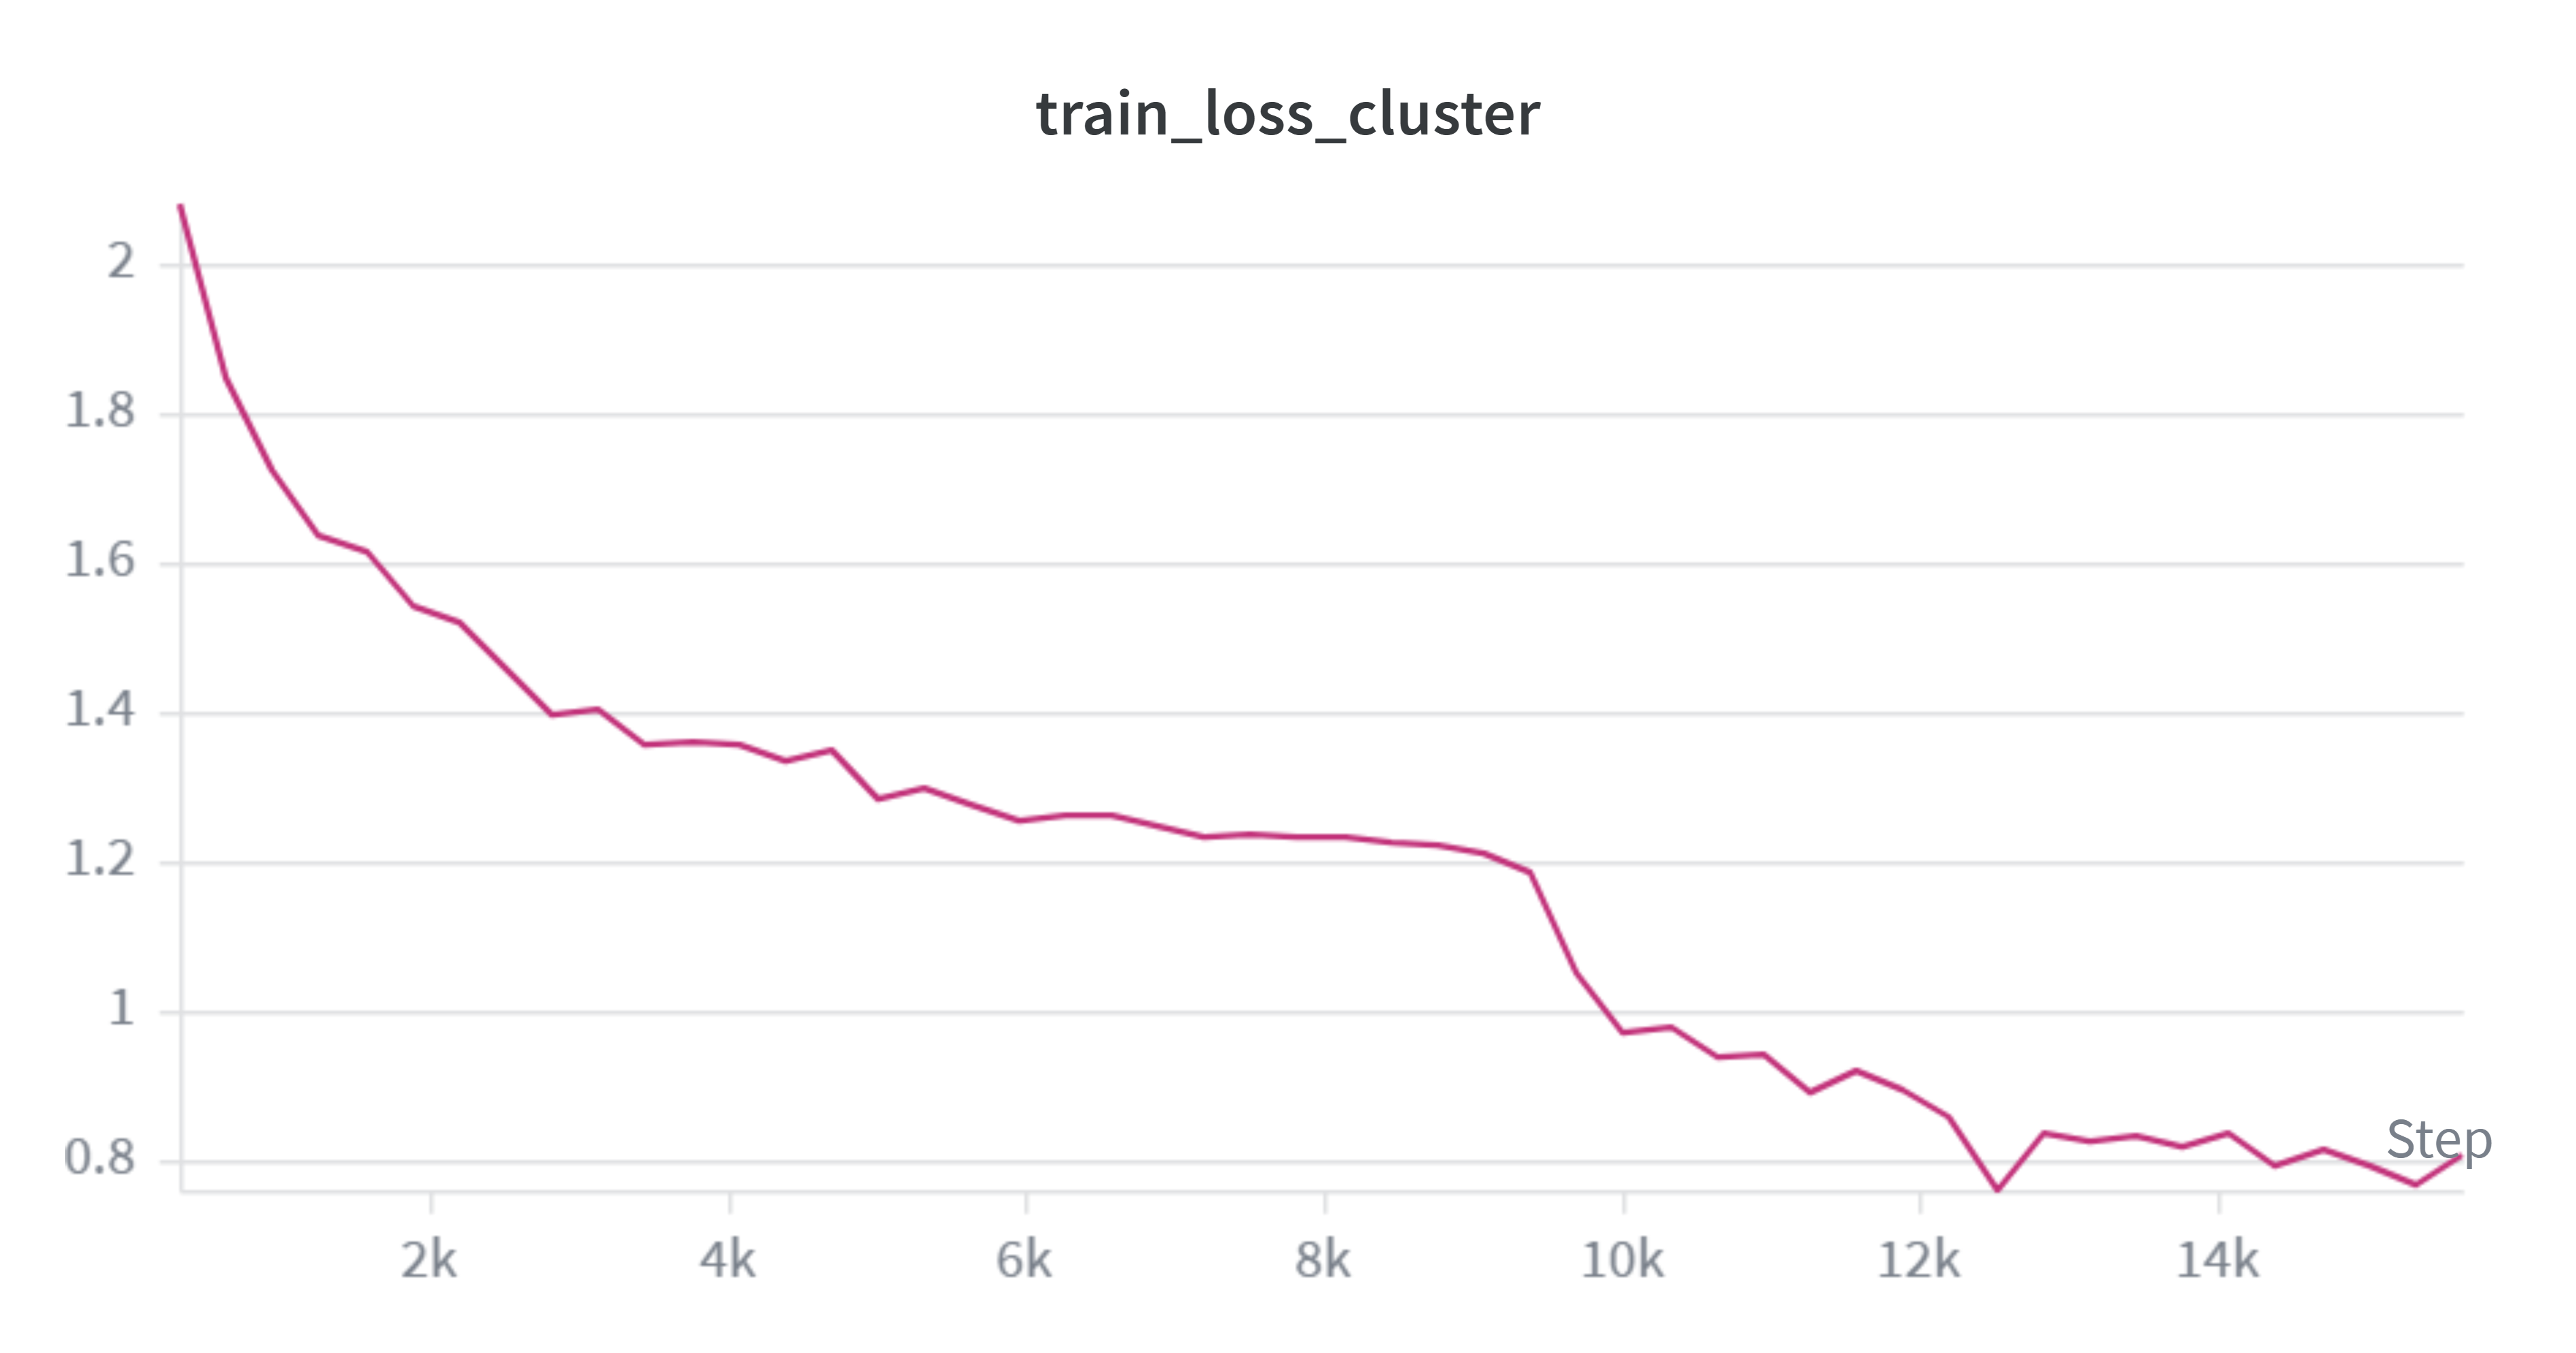
\includegraphics[width=0.95\linewidth]{figures/wandb/wb_train_loss.png}
\caption{Training loss.}
\end{subfigure}
\hfill
\begin{subfigure}[t]{0.45\linewidth}
\centering
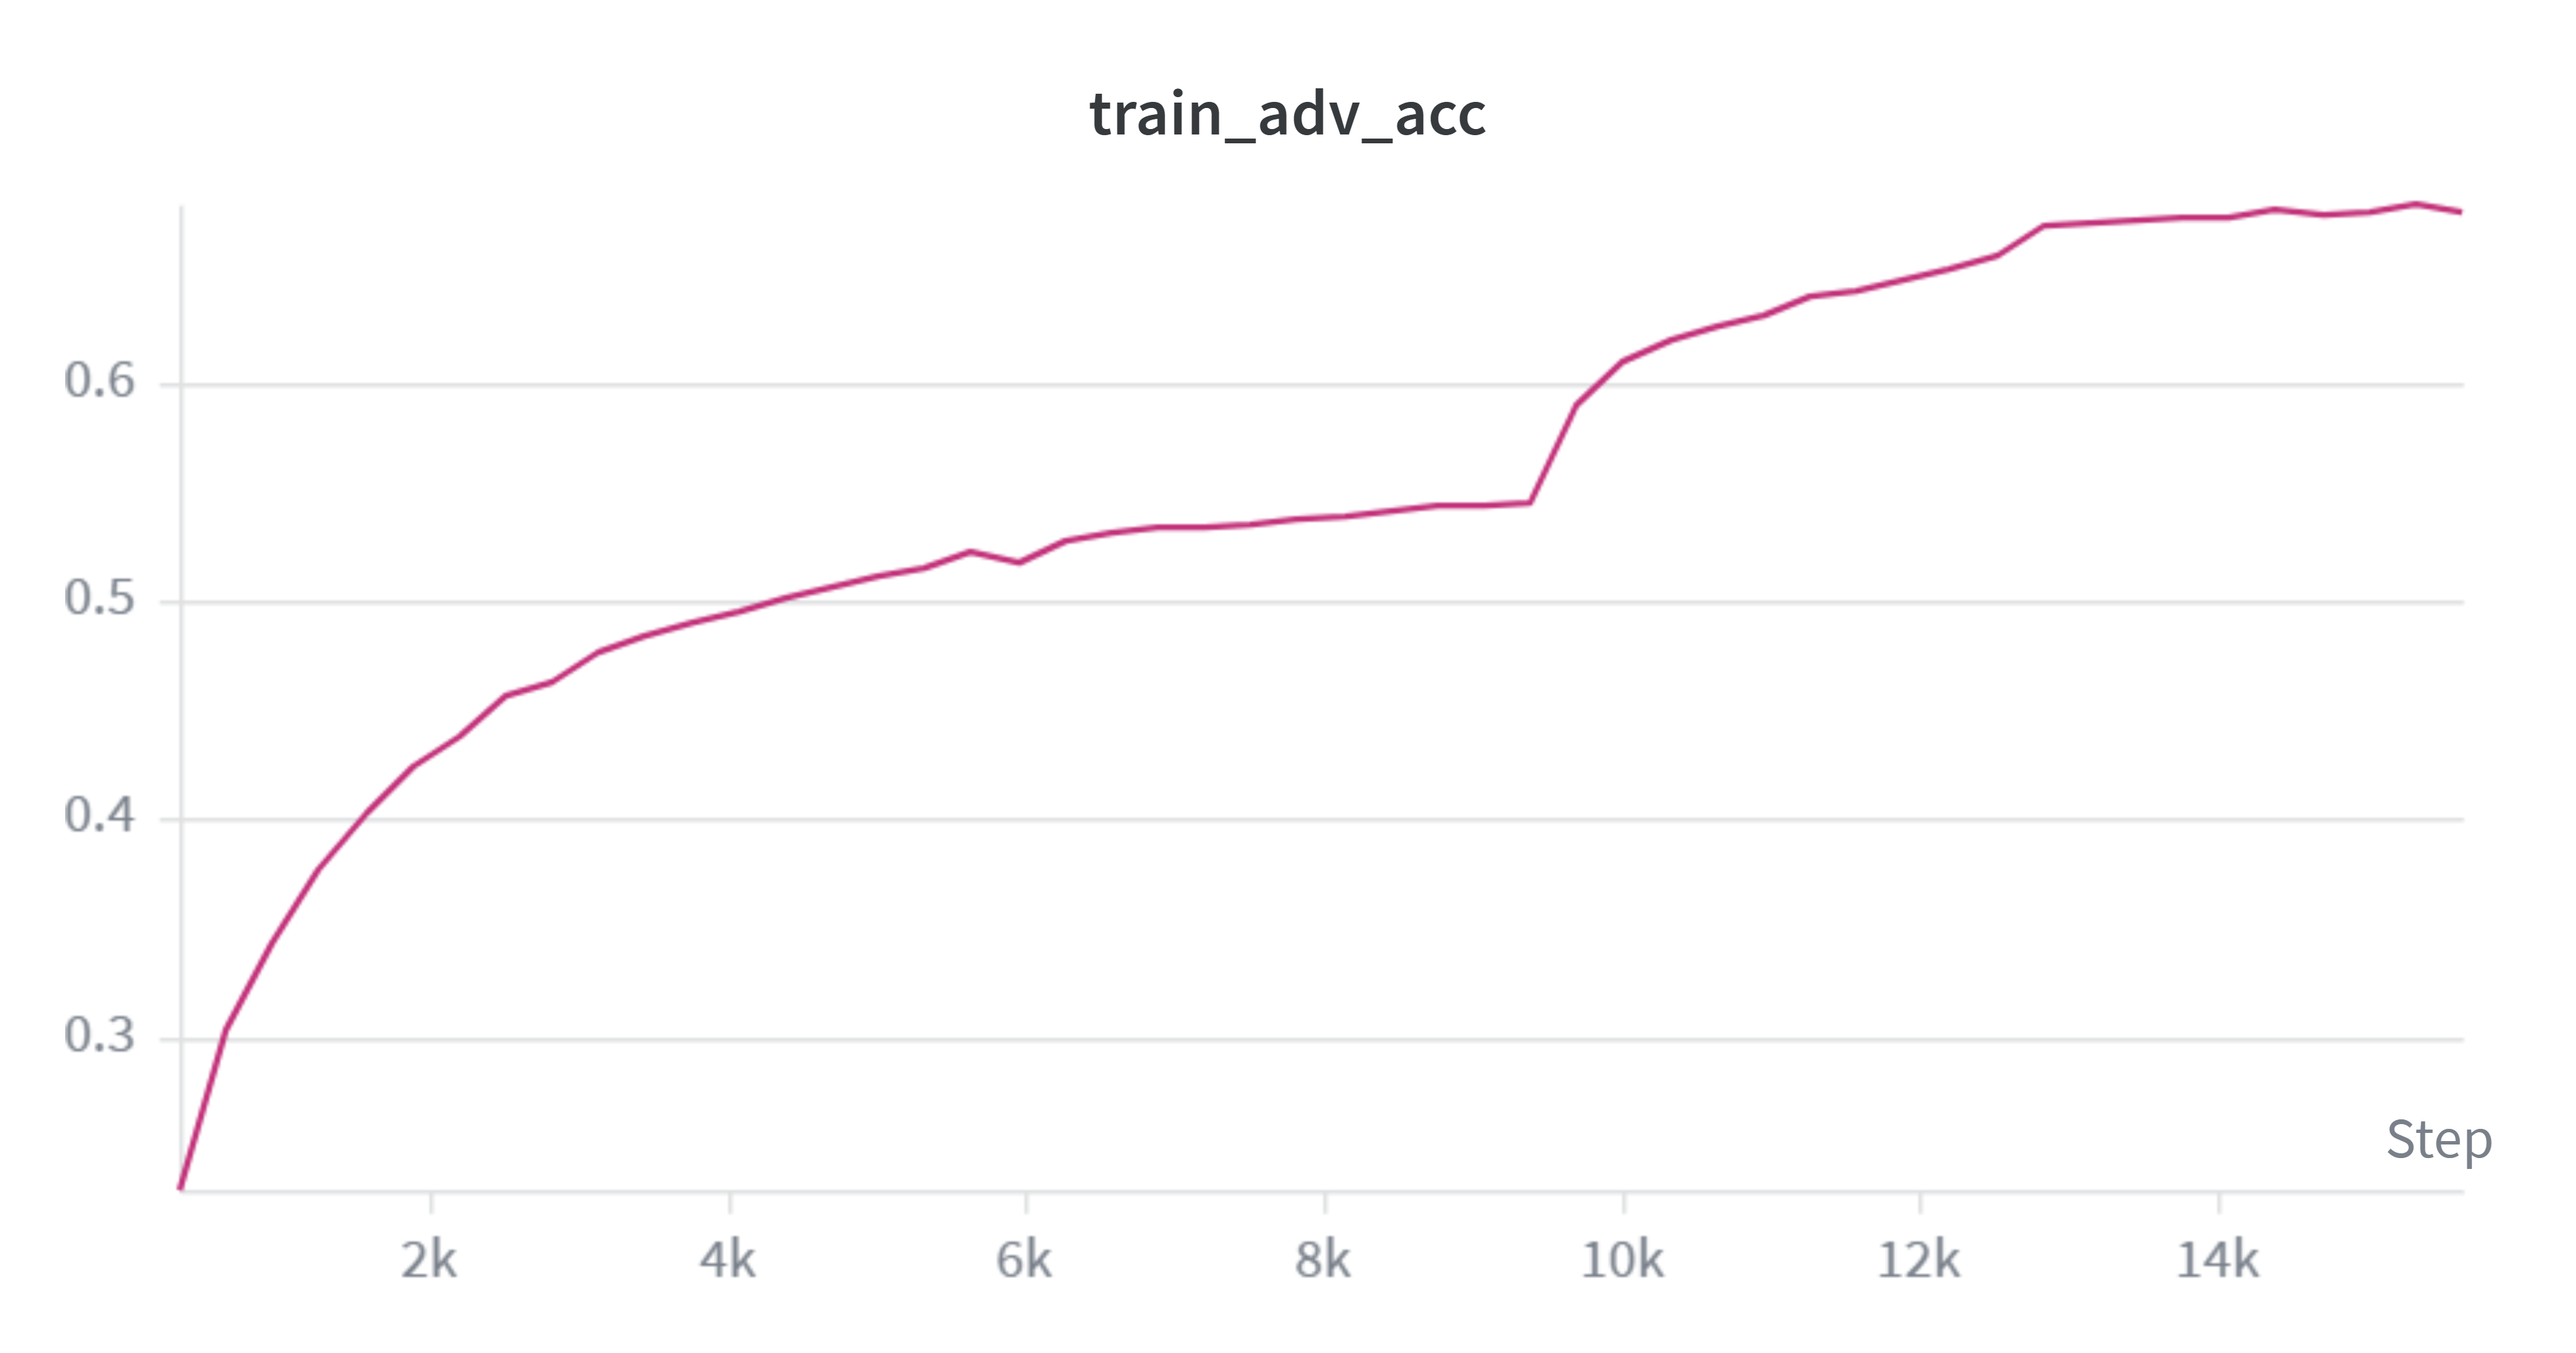
\includegraphics[width=0.95\linewidth]{figures/wandb/wb_train_acc.png}
\caption{Training accuracy.}
\end{subfigure}

\vspace{0.35em}
\begin{subfigure}[t]{0.45\linewidth}
\centering
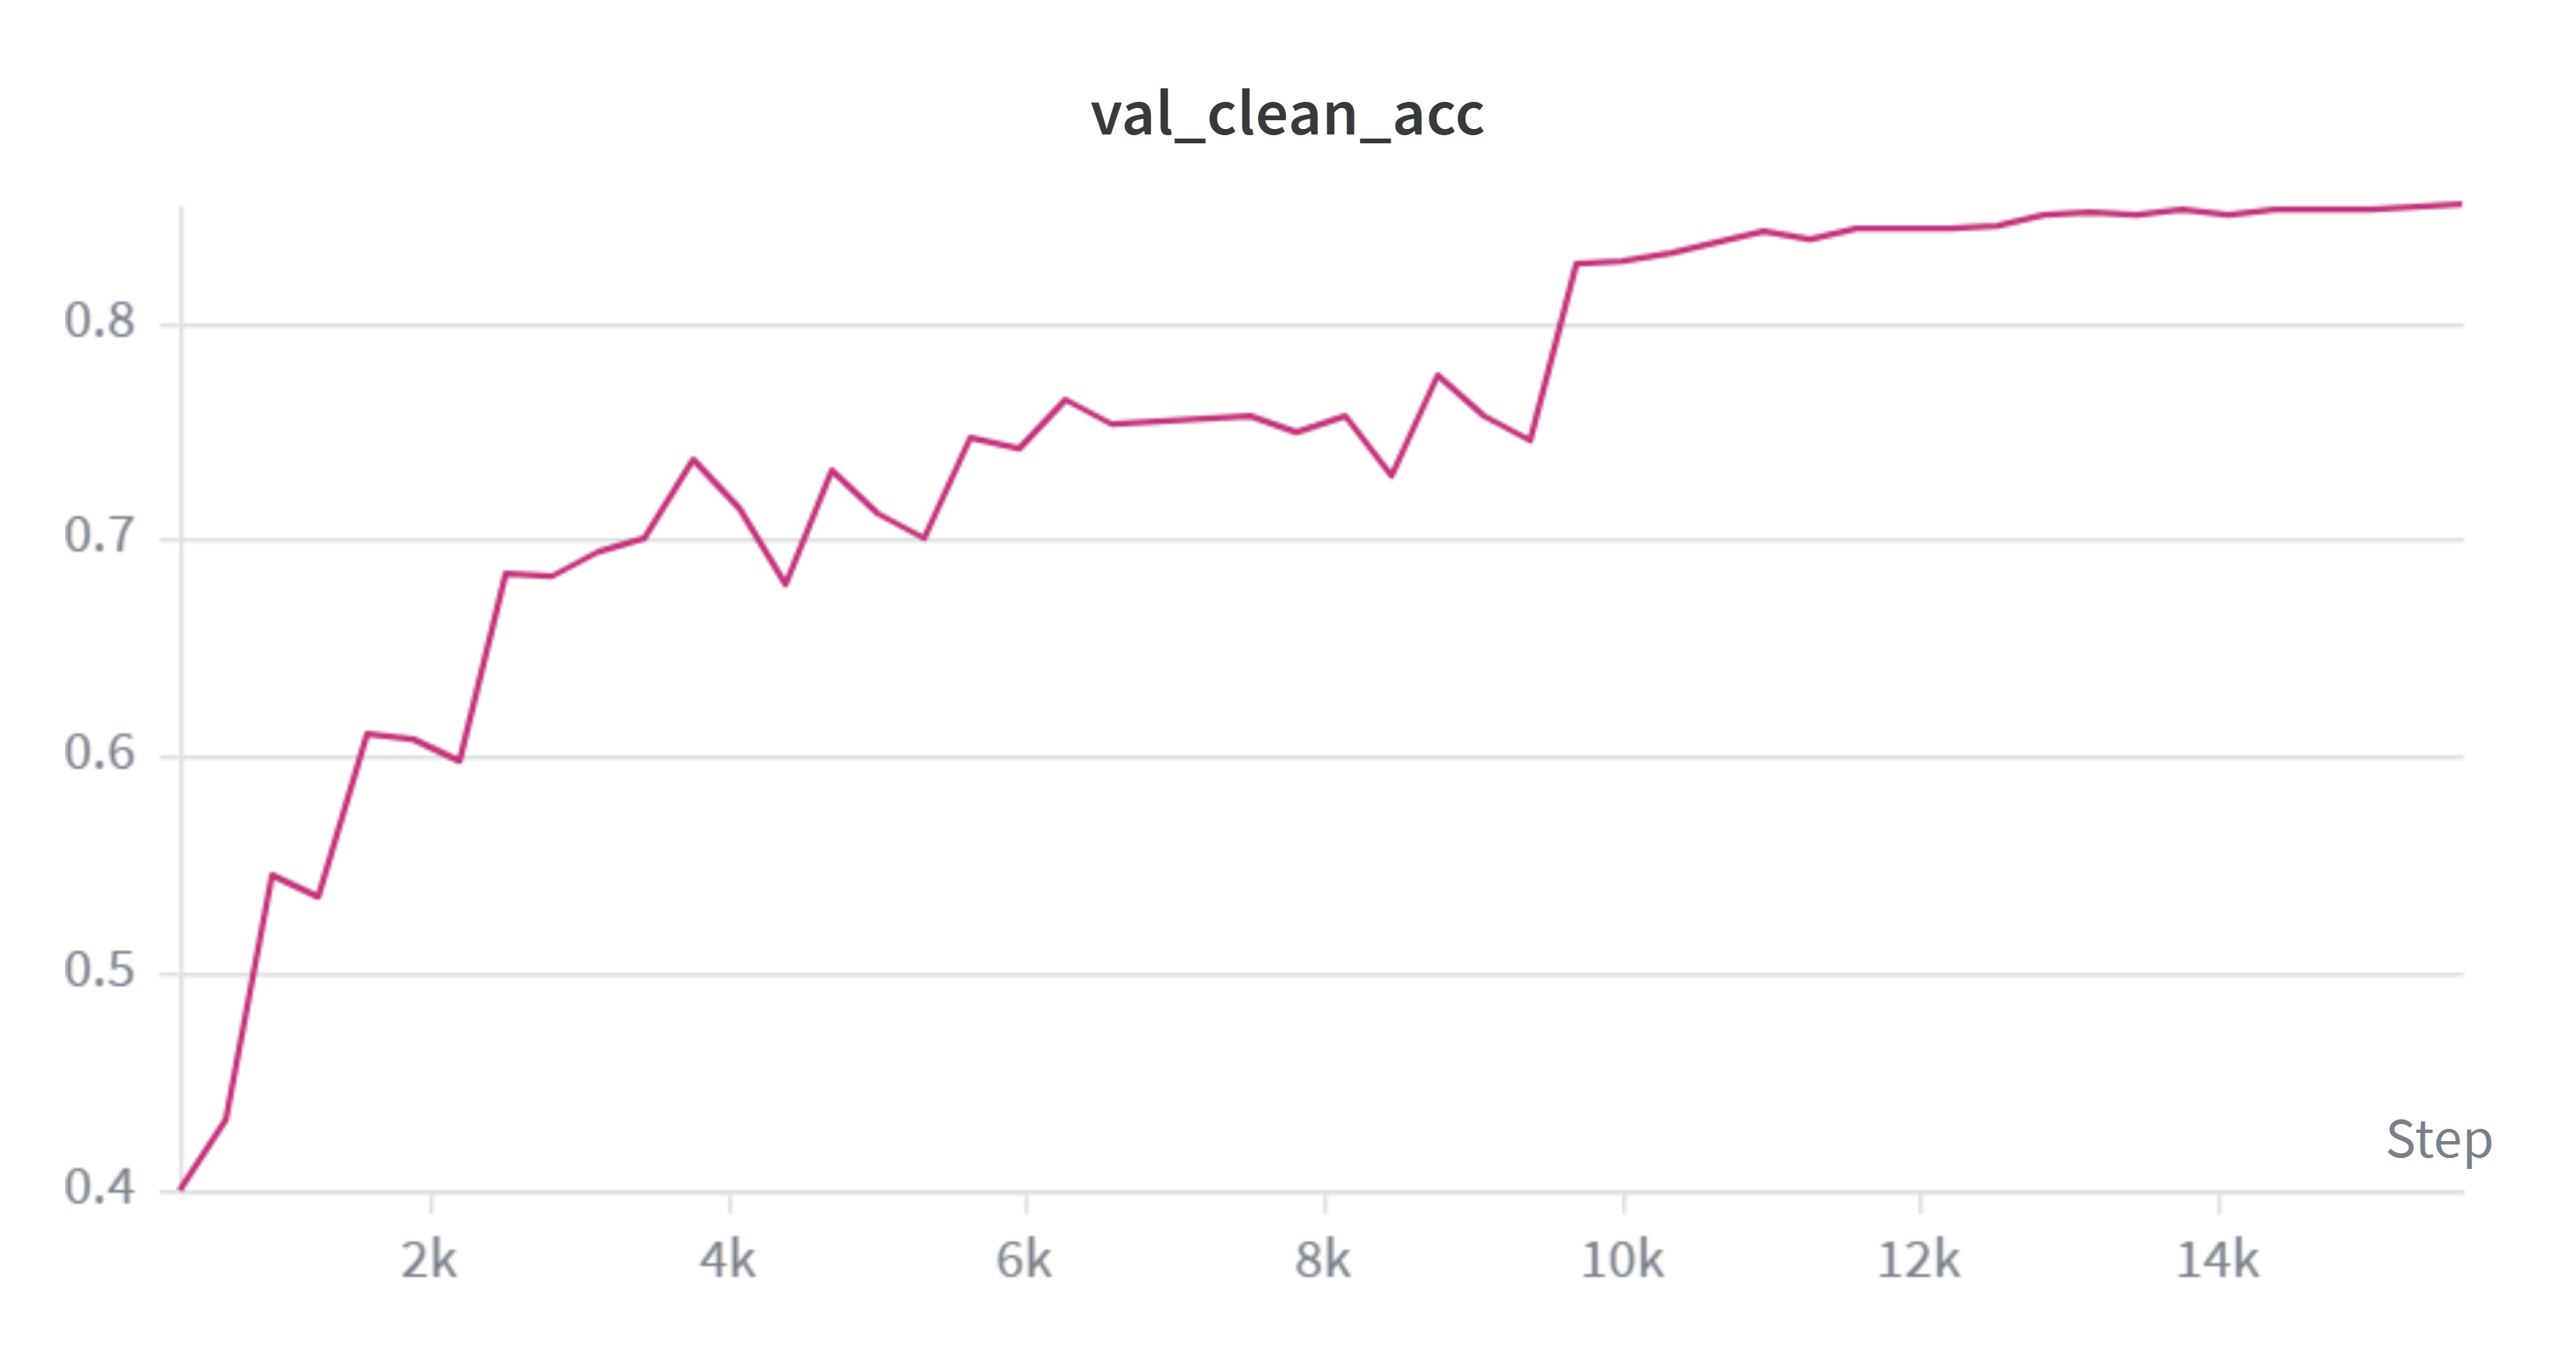
\includegraphics[width=0.95\linewidth]{figures/wandb/wb_val_clean_acc.png}
\caption{Clean validation accuracy.}
\end{subfigure}
\hfill
\begin{subfigure}[t]{0.45\linewidth}
\centering
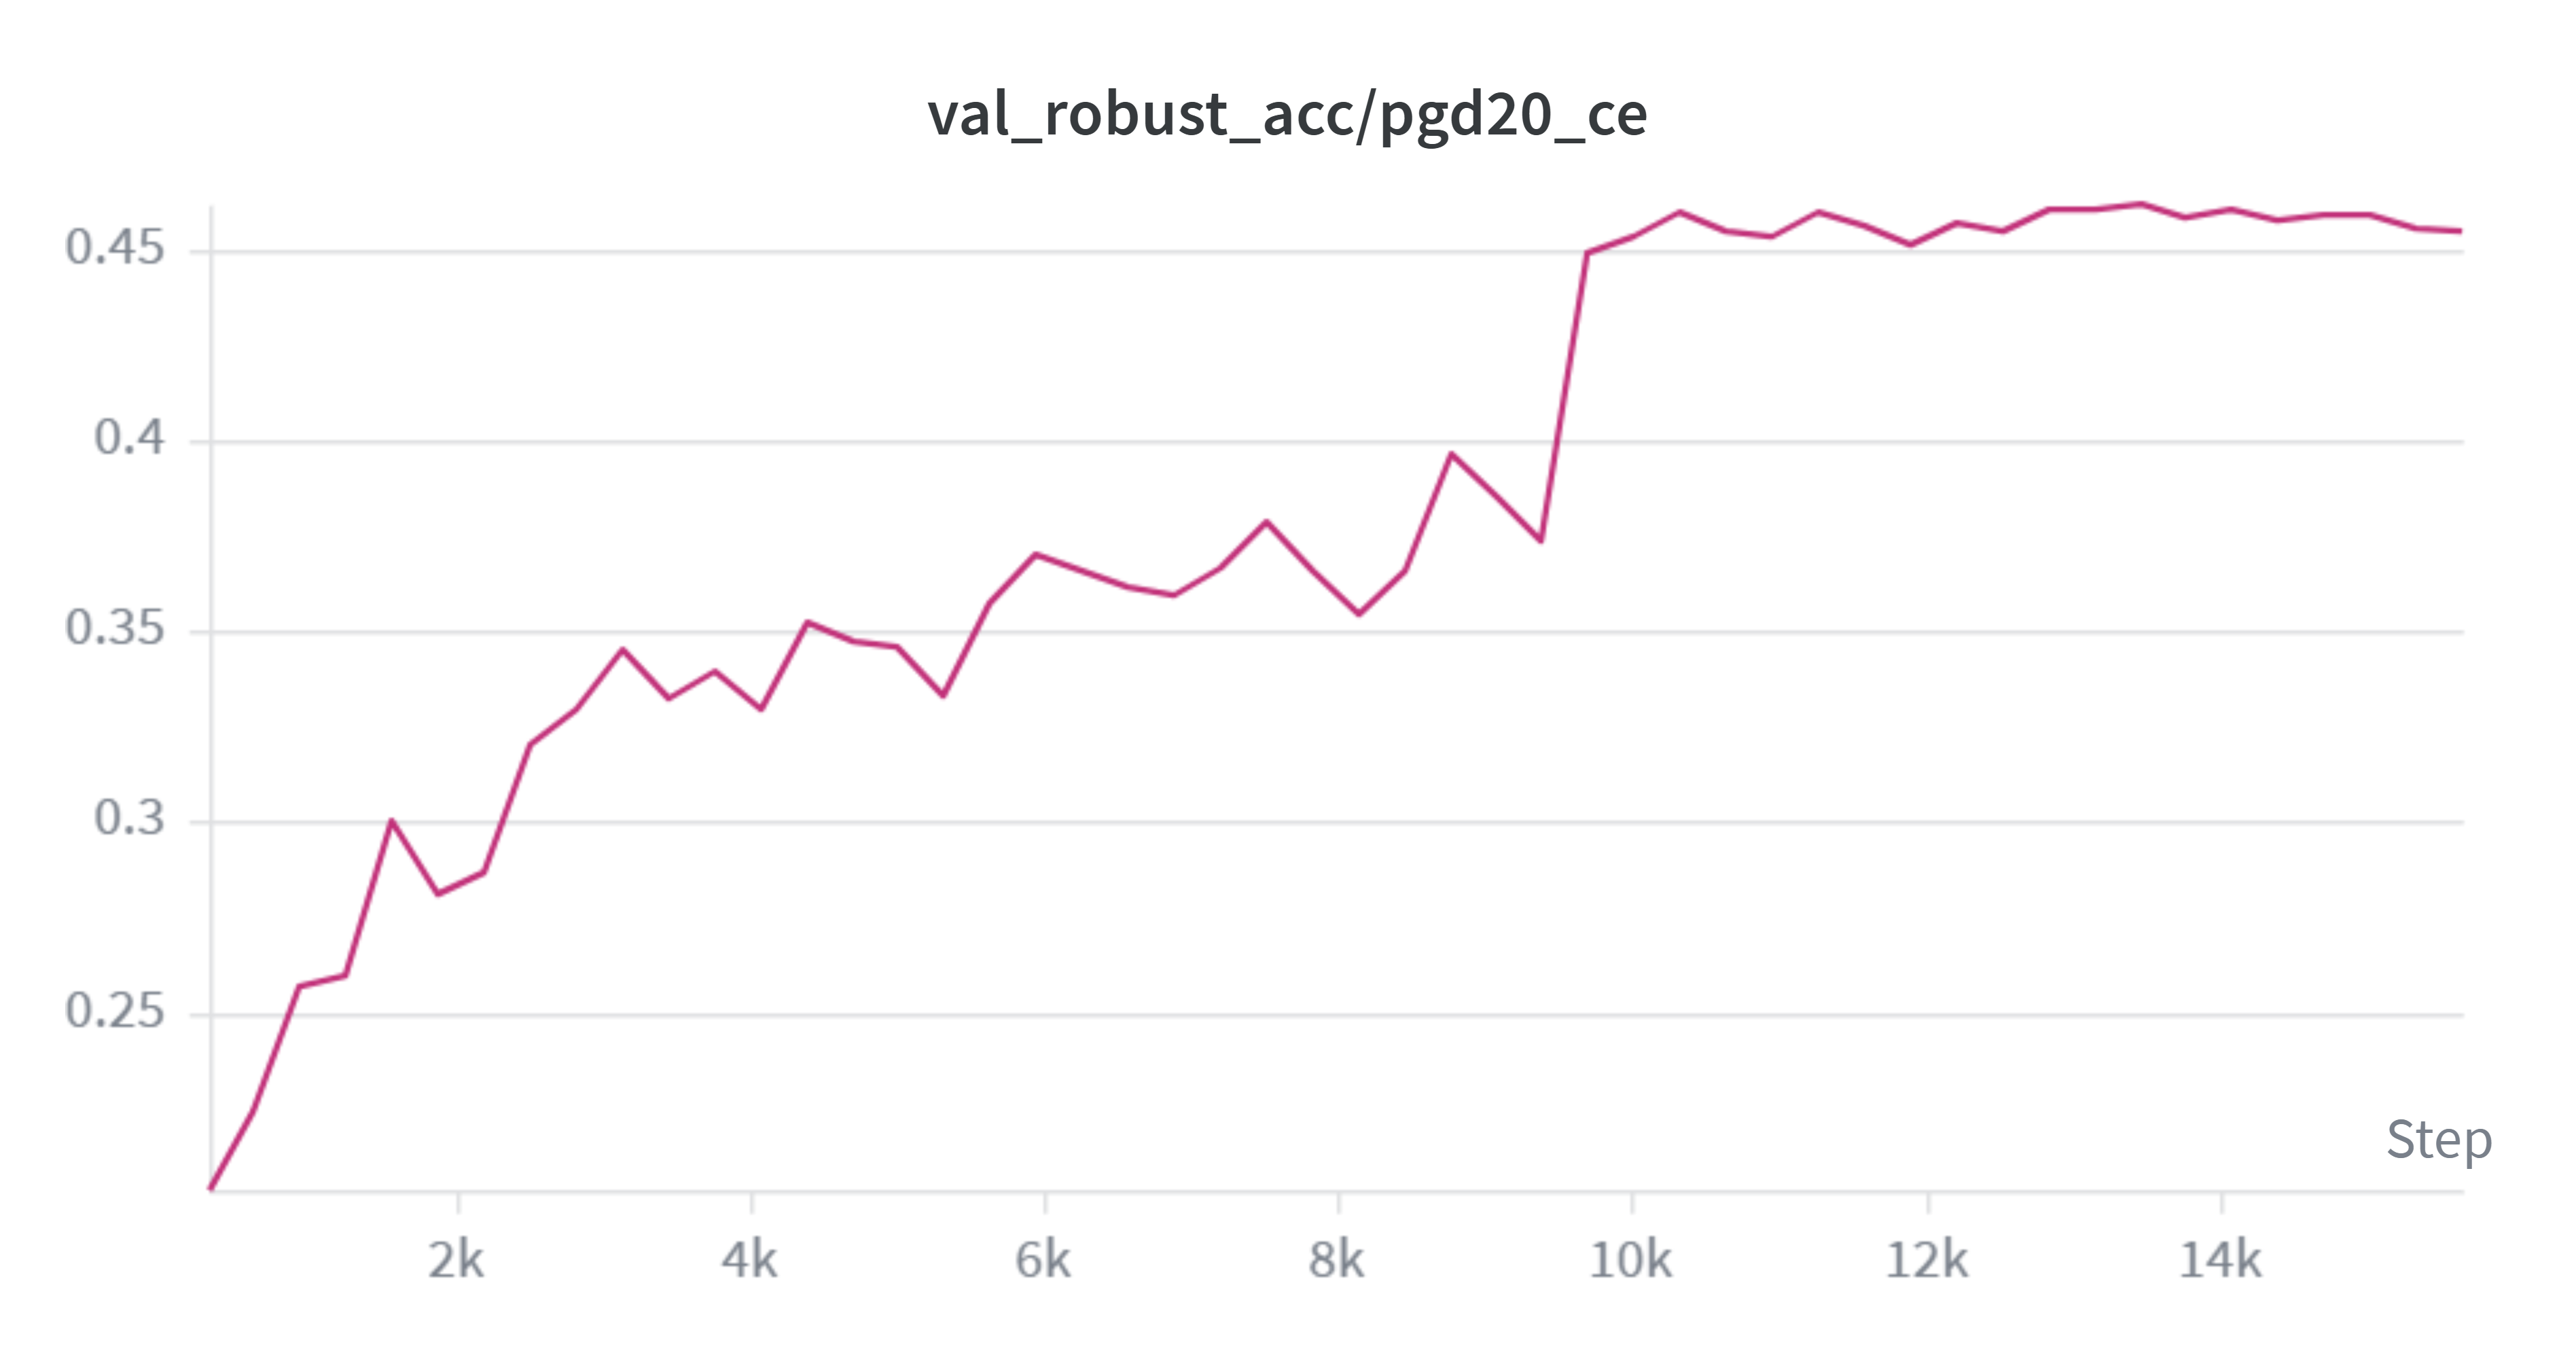
\includegraphics[width=0.95\linewidth]{figures/wandb/wb_pgd_linf_acc.png}
\caption{PGD-$\ell_\infty$ validation accuracy.}
\end{subfigure}

\vspace{0.35em}
\begin{subfigure}[t]{0.45\linewidth}
\centering
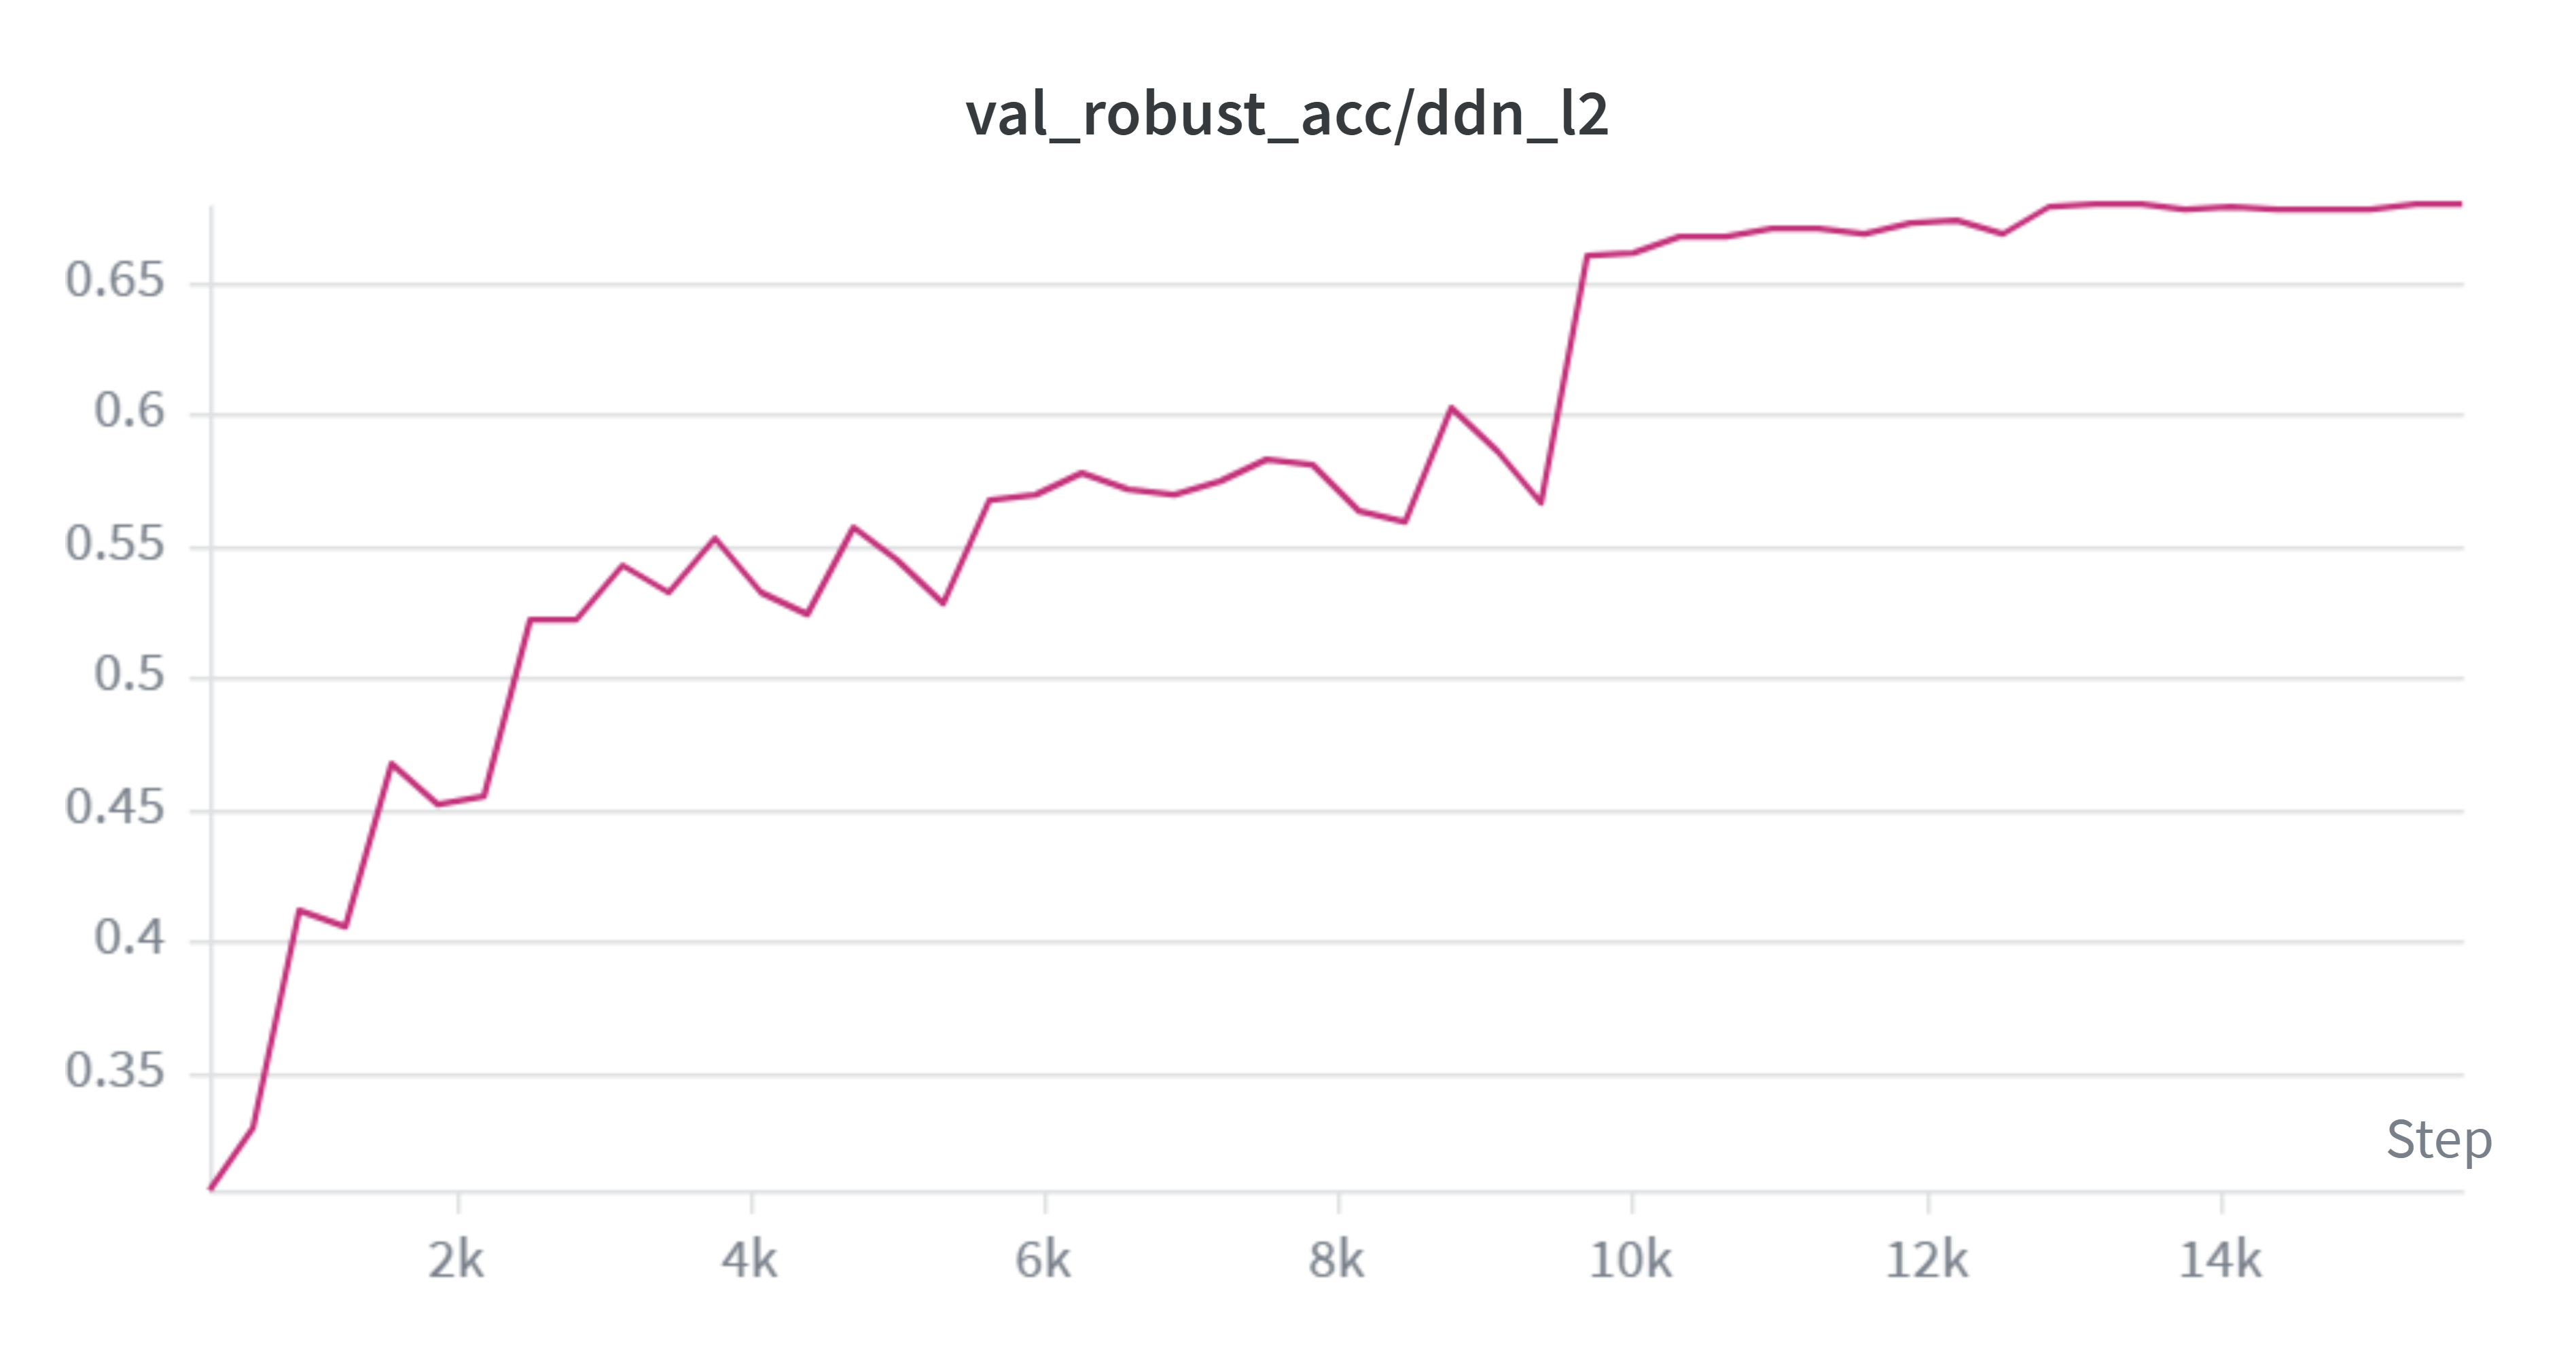
\includegraphics[width=0.95\linewidth]{figures/wandb/wb_ddn_l2_acc.png}
\caption{DDN-$\ell_2$ validation accuracy.}
\end{subfigure}
\hfill
\begin{subfigure}[t]{0.45\linewidth}
\centering
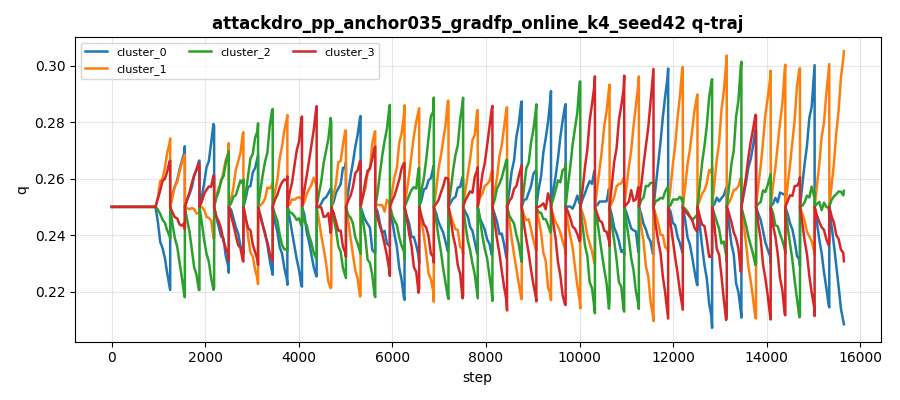
\includegraphics[width=0.95\linewidth]{figures/wandb/media_images_media_q_trajectory_15650_2752bccd0ffdd754ab89.png}
\caption{Group-weight trajectory.}
\end{subfigure}
\caption[W\&B dashboard exports]{Representative W\&B dashboard exports for experiment tracking. Panels (a)\textendash(e) track training loss, training accuracy, clean validation accuracy, and validation robustness under PGD-$\ell_\infty$ and DDN-$\ell_2$ during a training run. Panel (f) records the AttackDRO++ group-weight trajectory diagnostic. These exports document training telemetry and are not used as result evidence.}
\label{fig:app_wandb_core_metrics}
\end{figure}

% Goal: store run configuration, seed policy, split policy, attack configuration,
% training schedule, JSON logs, command lines if available, and compact config tables.

%===========================================================
% APPENDIX C: ADDITIONAL TABLES AND VISUALIZATIONS
%===========================================================

\chapter{Additional Tables and Visualizations}
\label{app:extras}

% Goal: store supplementary ablation tables, sweep summaries, training curves,
% qualitative grids, and plots that are not part of the main chapters.

\section{Adversarial Perturbation Visualizations}
\label{app:adv_visualizations}

\subsection{Grouped Adversarial Perturbation Visualizations}

Figure~\ref{fig:app_grouped_linf_adv_viz} and Figure~\ref{fig:app_grouped_l2_adv_viz} summarize adversarial examples and normalized perturbation heatmaps across the main \(\ell_\infty\) and \(\ell_2\) evaluation attacks. These figures are intended as qualitative support for the attack descriptions in Chapter~2; all heatmaps are normalized for visibility.

\begin{figure}[htbp]
\centering
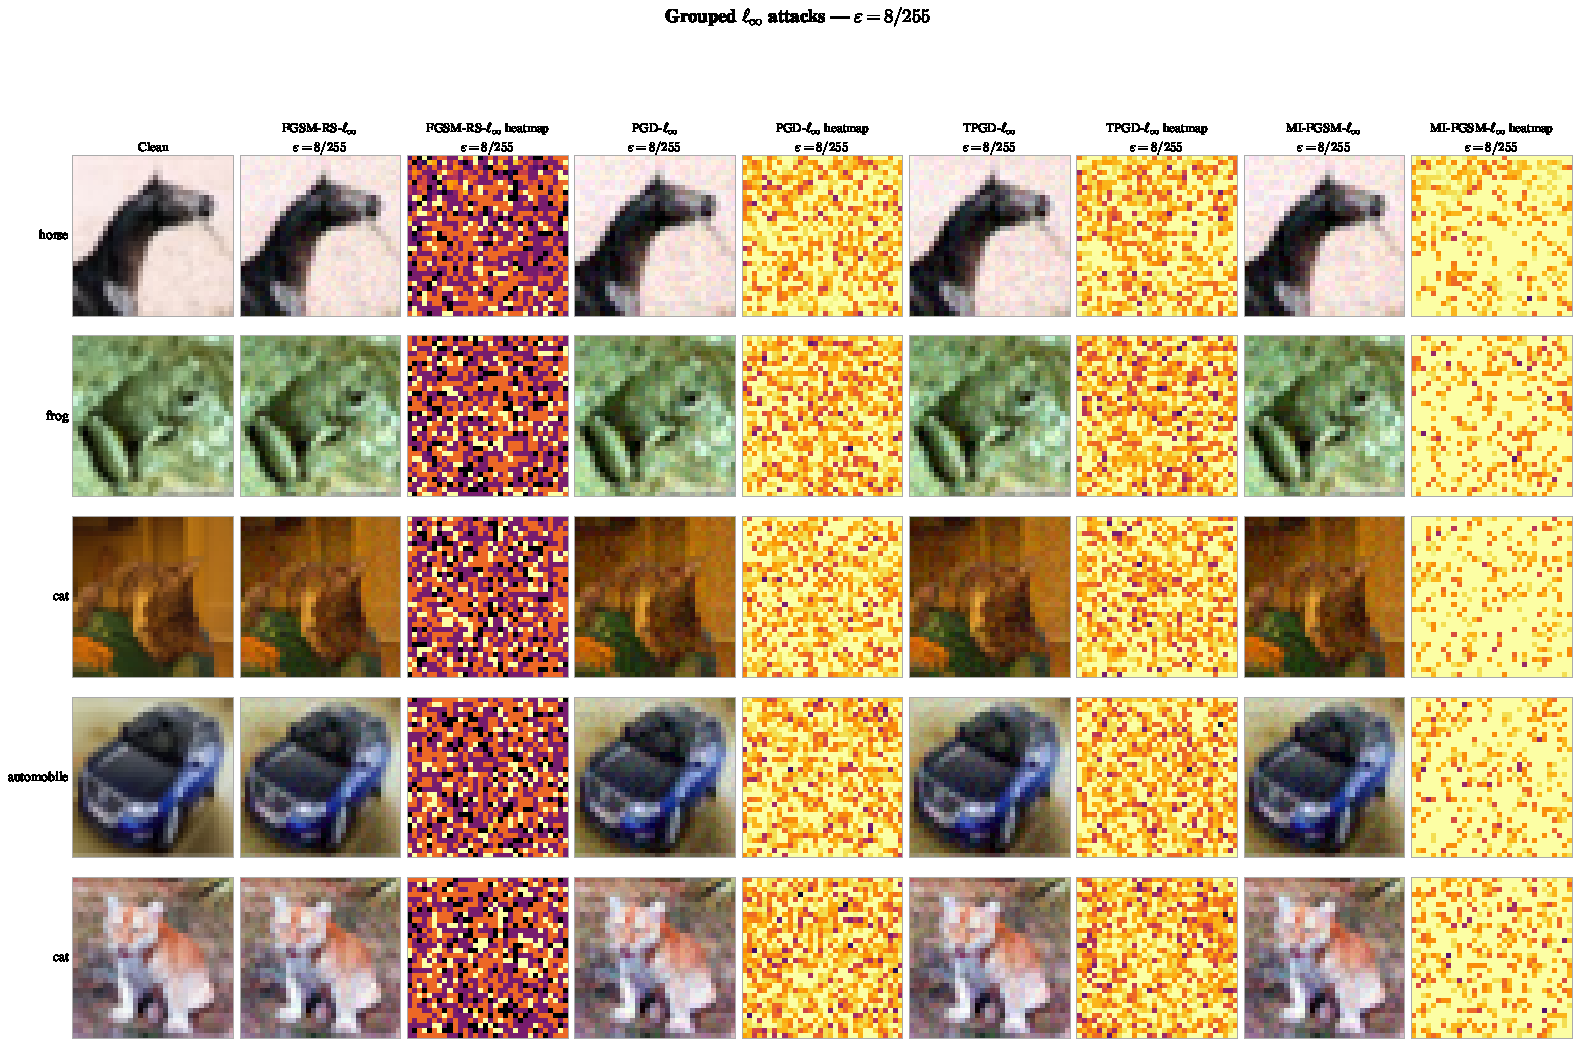
\includegraphics[width=0.90\textwidth]{figures/adv_viz/adv_grouped_linf.pdf}
\caption[Grouped \(\ell_\infty\) perturbation visualization]{Grouped \(\ell_\infty\) adversarial examples on CIFAR-10, with adversarial images and normalized perturbation heatmaps.}
\label{fig:app_grouped_linf_adv_viz}
\end{figure}

\begin{figure}[htbp]
\centering
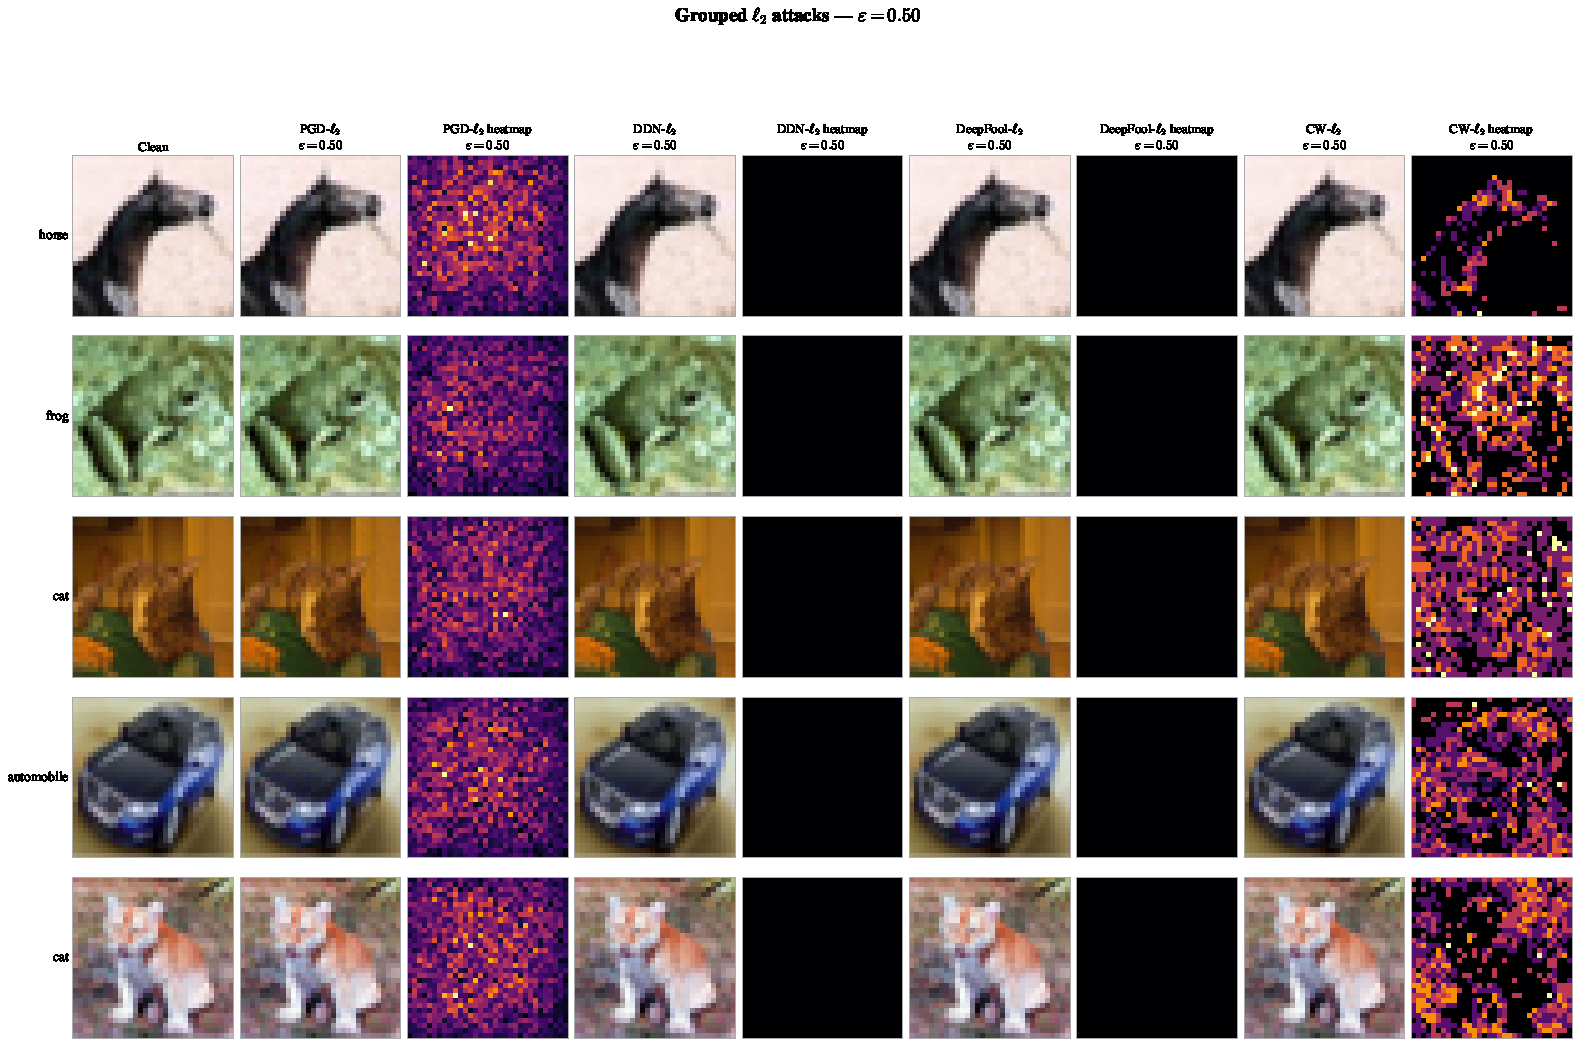
\includegraphics[width=0.90\textwidth]{figures/adv_viz/adv_grouped_l2.pdf}
\caption[Grouped \(\ell_2\) perturbation visualization]{Grouped \(\ell_2\) adversarial examples on CIFAR-10, with adversarial images and normalized perturbation heatmaps.}
\label{fig:app_grouped_l2_adv_viz}
\end{figure}

\begin{table}[H]
\centering
\caption[Supplementary WRN-28-10 architecture check]{Supplementary WRN-28-10 architecture check on CIFAR-10. Values are
robust accuracy (\%) from a single run and are therefore not included in the
main paired claims. Mean(8) and Worst(8) are computed over the eight
non-AutoAttack attacks; AutoAttack-$\ell_\infty$ is reported separately. Bold values indicate the best method for each metric.}
\label{tab:app_wrn2810_architecture_check}
\small
\setlength{\tabcolsep}{4pt}
\renewcommand{\arraystretch}{1.08}
\begin{tabular}{lccc}
\toprule
Method & Mean(8) $\uparrow$ & Worst(8) $\uparrow$ & AutoAttack $\uparrow$ \\
\midrule
Multi-AT
& \bestval{64.87}
& \bestval{47.99}
& \bestval{44.92} \\

AttackDRO++
& $64.68$
& $47.72$
& $43.16$ \\
\bottomrule
\end{tabular}
\end{table}

\begin{figure}[H]
    \centering
    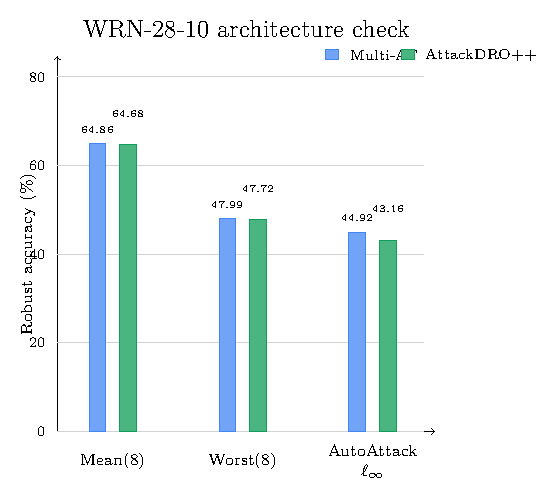
\includegraphics[width=0.75\linewidth]{figures/ablations/wrn2810_architecture_check.pdf}
    \caption[Supplementary WRN-28-10 architecture check]{Supplementary WRN-28-10 architecture check on CIFAR-10. Values are from a single run and are therefore not included in the main paired claims. Mean(8) and Worst(8) are computed over the eight non-AutoAttack attacks; AutoAttack-$\ell_\infty$ is reported separately.}
    \label{fig:app_wrn2810_architecture_check}
\end{figure}

%===========================================================
% APPENDIX D: COMPUTE RESOURCES AND ENVIRONMENT
%===========================================================

\chapter{Compute Resources and Environment Notes}
\label{app:compute}

The main experiments were executed through the Python and PyTorch pipeline
described in Chapter~\ref{chap:experimental_setup}.  Google Colab provided the
interactive GPU runtime, while Google Drive stored checkpoints, cached
adversarial examples, result CSV files, and exported figures.  The exact GPU
model available to a run was treated as execution metadata rather than an
experimental variable; model selection and statistical comparisons are based on
saved checkpoints and fixed evaluation scripts, not on wall-clock runtime.

The implementation stack used PyTorch and torchvision for training, TorchAttacks
and dedicated AutoAttack/DDN implementations for adversarial evaluation,
scikit-learn for MiniBatch K-means, and NumPy, pandas, matplotlib, and
SciencePlots for aggregation and figure generation.  Weights \& Biases was used
for telemetry and configuration tracking.  The source attack definitions,
evaluation attack suite, seed protocol, and reporting metrics are fixed in
Chapter~\ref{chap:experimental_setup}; this appendix records the compute context
only to avoid leaving the environment notes implicit.


\end{document}
